\documentclass[phd,icsa,twoside,logo,11pt]{infthesis}

\usepackage{amsfonts}
\usepackage{amsmath}
\usepackage{amsthm}
\usepackage[numbers]{natbib}
\usepackage[hidelinks]{hyperref}
\usepackage{cleveref}
\usepackage{graphicx}
\usepackage{listings}
\usepackage{xcolor}
\usepackage{calligra}
\usepackage[T1]{fontenc}
\usepackage[utf8]{inputenc}
\usepackage{tcolorbox}
\tcbuselibrary{theorems}
\usepackage{mathptmx}
\usepackage{enumitem}
\usepackage{pgfplots}
\usepackage{tabularx}
\usepackage{courier}
\usepackage{booktabs}
\usepackage{multirow}
\usepackage{rotating}
\usepackage{algorithm}
\usepackage[noend]{algpseudocode}

\usetikzlibrary{patterns}
\pgfplotsset{compat=1.13}

\newcolumntype{P}[1]{>{\centering\arraybackslash}p{#1}}

\hyphenpenalty=100000

\makeatletter
\newcommand{\tcb@cnt@definitionautorefname}{Definition}
\makeatother

\makeatletter
\newcommand{\tcb@cnt@notationautorefname}{Notation}
\makeatother

\newtcbtheorem[auto counter,number within=chapter]{definition}{Definition}{
label type=definition,
colback=white,
colframe=black,
fonttitle=\bfseries,
title={Definition \thetcbcounter}}{def}

\newtcbtheorem[auto counter,number within=chapter]{notation}{Notation}{
label type=notation,
colback=white,
colframe=black,
fonttitle=\bfseries,
title={Definition \thetcbcounter}}{not}

\definecolor{sh_comment}{rgb}{0.65, 0.00, 0.00 }
\definecolor{sh_keyword}{rgb}{0.15, 0.25, 0.25}
\definecolor{sh_string}{rgb}{0.08, 0.69, 0.08}

\lstset{
basicstyle         = \linespread{1}\ttfamily,
stringstyle        = \color{sh_string},
keywordstyle       = \color{sh_keyword}\bfseries,
commentstyle       = \color{sh_comment}\itshape,
numbers            = left,
numberstyle        = \scriptsize,
numbersep          = 10pt,
xleftmargin        = 1.5em,
frame              = lines,
framexleftmargin   = 1.5em,
framexbottommargin = 0em,
escapeinside       = {([}{])}
}

\lstdefinelanguage{CAnDL}
{
morekeywords = { Constraint, with, opcode, collect, include, function\_name,
                 data\_type, ir\_type, domination, strict\_domination,
                 calculated\_from, control\_origin, data\_origin, End },
morecomment  = [s]{\{}{\}}
}

\lstdefinelanguage{constraints}
{
morekeywords = { Constraint, with, and, or, at, as, End },
morecomment  = [s]{\{}{\}}
}

\lstdefinelanguage{LiLAC}
{
morekeywords = { HARNESS, IMPLEMENTS, Marshalling, PersistentVariables,
                 BeforeFirstExecution, AfterLastExecution, CppHeaderFiles,
                 INPUT, OUTPUT, COMPUTATION},
morekeywords = [2]{ CudaRead, CudaWrite, spmv_csr, Maximum, cuda, mkl,
                    dotproduct},
morekeywords = [3]{ out, in, size },
morecomment  = [s]{"}{"}
}


\title{Compiler Analysis as Constraint Programming\\
       for Idiomatic Heterogeneous Code Acceleration}
\author{Philip Ginsbach}

\abstract{%
    The end of Moores Law and the end of Dennard Scaling have required new
    approaches in hardware.
    In response, accelerator processors have become widespread, first in the
    form of general purpose graphics processing units (GPGPU) and now
    increasingly with even more deep learning accelerators.

    Heterogeneous computing platforms is the natural and necessary reaction to
    the scaling limitations of general purpose processors, but they pose a huge
    challenge to the surrounding software ecosystem.
    As opposed to microarchitectural improvements, existing software is not able
    to automatically profit from new acccelerators designs.

    A new hardware software contract is needed instead and heterogeneous
    hardware should become a responsibility of the compiler.
    While compilers have lagged behind the developments in the hardware domain,
    research into this area can profit from experience with multi-core
    processors.

    Auto-parallelizing compilers have failed to solve the problems and have only
    had major success for specific kernels and using auto-tuning.
    Heterogeneous computing is a superset of parallel computing and so an
    approach to fully automatically optimize code is unlikely.

    At the same time, a library and DSL based approach has been successful,
    however fails to become mainstream due to adoption cost.
    What is promising therefore is a combination of hand-optimized libraries
    together with compiler automatisms.

    This requires a disruptive improvement in compiler analysis capabilites.
    The detection of higher level algorithmic structures in compilers has been
    investigated before, but established approaches cannot scale to what
    this challenge requires.
    Syntactic matching on programming languages has become
    unviable for the complexities of both modern programming languages and
    complex code bases.

    Instead, this thesis develops an entirely novel approach based on concepts
    from constraint solving, building a pragmatic methodology for detecting
    complex algorithmic structures -- computational idioms.
}

\begin{document}
\begin{preliminary}
\maketitle
\begin{acknowledgements}

\end{acknowledgements}
\begin{declaration}
    I declare that this thesis was composed by myself, that the work contained
    herein is my own except where explicitly stated otherwise in the text, and
    that this work has not been submitted for any other degree or professional
    qualification except as specified.
    Some of the material used in this thesis has been published in the following
    papers:

    \begin{itemize}
    \small
        \item Philip Ginsbach and Michael F.\ P.\ O'Boyle.\\
              {\bf Discovery and Exploitation of General Reductions: A
              Constraint Based Approach}.\\
              {\em Proceedings of the 15th Annual International
               Symposium on Code Generation and\\Optimization (CGO), 2017}
        \item Philip Ginsbach, Lewis Crawford and Michael F.\ P.\ O'Boyle.\\
              {\bf CAnDL: A Domain Specific Language for Compiler Analysis}.\\
              {\em Proceedings of the 27th International Conference on
               Compiler Construction (CC), 2018}
        \item Philip Ginsbach, Toomas Remmelg, Michel Steuwer, Bruno Bodin,
              Christophe Dubach and\\Michael F.\ P.\ O'Boyle.\\
              {\bf Automatic Matching of Legacy Code to Heterogeneous APIs: An
              Idiomatic Approach}.\\
              {\em Proceedings of the 23rd International Conference on
               Architectural Support for\\Programming Languages and Operating
               Systems (ASPLOS), 2018}
        \item Philip Ginsbach, Bruce Collie and Michael F.\ P.\ O'Boyle.\\
              {\bf Automatically Harnessing Sparse Acceleration Libraries}.\\
              In: {\em ???, 2019}
    \end{itemize}

    \par
\vspace{1in}\raggedleft({\em Philip Ginsbach})
\end{declaration}
\tableofcontents
\end{preliminary}
\chapter{Introduction}
    \label{chapter:introduction}
    \section{The Emergence of Heterogeneous Computing}

    For several decades, from the 1970s until the early 2000s, advances in
    processor development followed Moore's Law \citep{4785860} and
    Dennard Scaling \citep{1050511}.
    The density of integrated circuits doubled every two years,
    and this allowed increased clock frequencies while maintaining
    steady power consumption.
    These conditions enabled continual processor improvements that were driven
    primarily by rising clock frequencies and microarchitectural refinements,
    enabling ever faster computations.

    The physics-driven nature \citep{Hutcheson2018Moore} of these advances in
    hardware has had important implications for software development.
    Not only did the performance of computers improve exponentially, but these
    performance gains were in the form of direct speedups, available to all the
    already existing programs.
    The primary interfaces between software and hardware - the instruction set
    architectures of processors - evolved gradually and with few
    paradigmatic changes \citep{8310168}.
    This is best exemplified by the pervasive x86 instruction set architecture,
    which still retains backward compatibility with its initial version from
    1978, and dominates desktop processors to this day.
    Therefore, software developers and users could rely on ever-increasing
    performance from hardware progress alone, without any intervention.

\subsection{Via Multi-Processing to Heterogeneity}

    This continual progress started breaking down around 2005 with the apparent
    end of Dennard Scaling \citep{6307773}.
    While the shrinking of transistors continued, this no longer enabled
    proportionally increased clock frequencies with the same power budget.
    Instead, processor designers started using the increasing transistor
    budget for additional processor cores.
    This shift toward multi-processing has left a deep mark on software
    development.
    New programming paradigms and languages, annotation systems, programming
    interfaces, libraries and compiler techniques are still being developed to
    address the challenges of parallel computing.

    In recent years, transistor scaling has slowed significantly.
    In response to the breakdown of both Dennard Scaling and Moore's Law, the
    hardware industry has turned toward architectural innovation
    \citep{7878935}.
    In particular, there is a trend toward specialised processor cores that work
    in tandem as a heterogeneous system.
    Such dedicated processor cores outperform general-purpose cores on
    specific tasks.
    Furthermore, as heat dissipation has become a major challenge,
    simultaneously powering all transistors is often unviable, meaning that
    different processor cores have to be masked out dynamically at runtime
    (``dark silicon'') \citep{6307773}.
    Disabling a subset of a homogeneous multi-core system renders some of its
    cores redundant.
    However, specialised cores can improve the system performance overall even
    if they are disabled most of the time and only used for the specific tasks
    at which they excel.

\section{The Diminished Role of Traditional Compilers}

    Heterogeneous computing can help overcome the scaling limitations of
    homogeneous, general-purpose processors.
    However, it also poses a challenge to the associated software ecosystem,
    putting into question many of the achievements in portability and longevity
    of programs that are taken for granted in modern computing \citep{8719512}.
    Existing software does not automatically benefit from entirely new
    accelerator designs in the way that it profited from the continuous
    improvements of established architectures.
    Where programs previously performed better on each succeeding hardware
    generation, new accelerators arrive with novel and incompatible interfaces.

    In particular, this new hardware landscape greatly diminishes the scope of
    responsibilities and impact that traditional compilers for languages such as
    C, C++ and Fortran can have.
    Such compilers used to be responsible for orchestrating
    program execution on the entirety of available computing resources.
    They are now generally limited to only targeting the relatively small
    homogeneous fraction of processor cores directly.

\subsection{Libraries and Domain-Specific Languages}

    In order to reach peak performance on rapidly evolving and highly parallel
    hardware, novel programming paradigms built around libraries and
    domain-specific languages have emerged.
    They succeed in utilising heterogeneous hardware in situations where
    traditional compilers fail.

    Two examples display the diversity of these approaches.
    Firstly, \citet{Ragan-Kelley2013Halide} developed the domain-specific
    language Halide for image processing.
    The Halide toolchain is able to generate fast code for heterogeneous
    platforms by focusing on a well-understood class of computations and by
    using a restrictive program representation.
    After tuning programs for particular platforms, it outperforms
    hand-optimised code, demonstrating the advantage of domain-specific compiler
    optimisation under circumstances of constrained semantics.

    Secondly, Basic Linear Algebra Subprograms (BLAS)
    \citep{2002:USB:567806.567807}, a standard for library function interfaces
    going back to \citet{Lawson:1979:BLA:355841.355847} in the 1970s, have been
    implemented for most accelerators.
    These implementations are widely used and offer unrivalled performance.
    Some versions are provided directly by hardware vendors to support
    accelerators \citep{mkl,cublas,clblas,apl,qml}, while others originate as
    academic projects \citep{Wang:2013:AAG:2503210.2503219}.
    These competing implementations use a plethora of approaches to achieve as
    close to peak performance as possible.
    These includes manually written assembly code, but also highly advanced
    code generation techniques, custom program representations and many more.

\subsection{The Consequences of the Decline of Compilers}

    Domain-specific languages and library interfaces make the full performance
    of heterogeneous systems accessible to programs.
    These success stories, however, leave significant problems unaddressed.
    The adoption costs are high, requiring application rewrites for
    accelerators.
    This coincides with often uncertain long-term prospects and minimal
    cross-platform portability.
    Even in the case of the agreed-upon BLAS standard -- arguably the best case
    scenario -- adoption of novel implementations is non-trivial in practice,
    due to the frequently encountered interface extensions for managing device
    handlers and memory synchronisation.
    For academic-backed domain-specific languages like Halide, on the other
    hand, complete rewrites are required in entirely novel software ecosystems,
    with an unclear future of support.

    On homogeneous systems, programmers could rely on compilers for existing
    programming languages to evolve in lockstep with processor development.
    For example, even decades-old C++ source code compiles into efficient
    programs for the newest generation of x86 processors.
    Libraries and domain-specific languages are useful on homogeneous systems
    for achieving absolute maximum performance, but they become essential only
    in the context of heterogeneity.
    Therefore, the pervasive requirement for domain specific-languages and
    libraries only arises because compilers are unable to map programs onto
    specialised cores.
    Instead, compilers are increasingly downgraded to merely coordinating the
    launch of core workloads in the form of computational kernels, which are
    then executed as separate and opaque programs.

    It may appear that, for example, a C++ or Java compiler cannot
    be provided for a typical graphics processor.
    After all, most graphics processors have hardware limitations that prevent
    them from implementing the entire language standard.
    Indeed, many accelerators are even further from Turing complete.
    However, this should not prevent a partial compiler.
    Such a partial compiler would compile fitting program parts for accelerators
    and utilise a fallback system for the remainder of the program.
    After all, that is precisely the result achieved with libraries and
    domain-specific languages, and likely the desirable outcome.
    Despite the apparent convenience of such an approach, the next section gives
    reasons why such a scheme has not been championed so far.

\section{Host Compilers and Kernel Compilers}
\label{sec:hostkernel}

    While mainstream compilers for languages such as C/C++, Fortran or Java
    generally fail to exploit the full performance of heterogeneous systems, a
    specific class of compilers already plays an essential role in
    targeting heterogeneous hardware.
    Many of the kernel programs that remain opaque to the application compilers
    are themselves products of other, specialised compilers.
    This necessitates a distinction between {\em host compilers} and {\em kernel
    compilers}.
    This distinction is mirrored by the differences between {\em host languages}
    and {\em kernel languages}.
    Host compilers translate full programs written in host languages -- such as
    the previously mentioned C/C++, Fortran and Java -- while kernel
    compilers handle small computational kernels that are expressed in dedicated
    domain-specific programming languages.
    The two classes of compilers have developed differently.
    Kernel compilers successfully apply many of the techniques that are severely
    limited on host compilers
    \citep{Murphy2014LimitsOD,Maleki:2011:EVC:2120965.2121464}.
    They reason automatically about parallelism
    \citep{Steuwer:2017:LFD:3049832.3049841}, are more successful at accurately
    modelling data dependencies \citep{Baghdadi:2019:TPC:3314872.3314896}, and
    incorporate iterative compilation techniques
    \citep{Ansel:2014:OEF:2628071.2628092}.

    This is made possible by a combination of factors that uniquely apply to
    kernel compilers:
    Smaller programs allow for more expensive compilation techniques;
    more restrictive languages and intermediate representations allow for
    stronger reasoning;
    abstractions in kernel compilers can be customised for the exact hardware
    architecture of accelerators;
    and domain knowledge from areas such as image processing can be directly
    embedded in custom compiler technology, without requiring their validity
    on generic programs.
    Furthermore, kernel compilers often run in more controlled environments,
    with less need for predictability, reproducibility, and stability.
    The range of input programs might even be small enough to ship them in an
    already compiled form, making the compiler merely a tool in a
    library-implementation process.

    As host compilers operate under less forgiving conditions, it is
    unsurprising that they have lagged behind these developments.
    Because they cannot rely on such a restricted environment, host compilers
    are unable to match the optimisation capabilities of kernel compilers.
    Domain-specific compilers and languages, as well as libraries, have
    therefore not been championed only because their restricted program
    spaces match the capabilities of particular heterogeneous accelerators.
    The restricted environment also makes them intrinsically more powerful and
    able to generate better code.

    Hybrid approaches, such as OpenCL, reinforce these hypotheses.
    The language is domain-specific in its expression of parallelism, but
    otherwise designed to be quite general-purpose.
    Compilers are provided for many structurally different processors.
    However, as a consequence of being a relatively unrestricted language, the
    compilers often underperform and the language is notoriously lacking in
    performance portability \citep{Falch:2015:MLB:2863697.2864570}.
    Partial compilers that require the same compromises as OpenCL -- being
    unable to utilise the restricted nature of input programs -- would surely
    suffer the same shortcomings.

\subsection{The Spectrum of Specialisation}

    General-purpose programming languages, domain-specific languages and
    accelerator libraries exist on a spectrum of specialisation.
    \Cref{specialgradient} provides some intuition about this spectrum by
    gauging the places of popular languages and compute libraries in it.
    On the far left are versatile general-purpose languages, such as C++ and
    Fortran.
    Moving right, flexibility is gradually lost, with BLAS libraries at
    the end providing only fixed-function computations.
    However, the restricted semantics allow for increased optimisation
    capabilities in return.

    It is necessary to clarify what is meant by optimisation potential in this
    context and how it differs from raw performance.
    C++ is, of course, very suitable for manual optimisation and renowned as a
    low-overhead, high-performance language.
    However, it is difficult for compilers to apply deep structural changes to
    C++ programs correctly.
    Maintaining the semantics of BLAS routines, on the other hand, is viable
    with many structurally different implementation approaches.
    Therefore, C++ is fast because of its low overhead, and because C++
    programmers write programs with performance in mind.
    By contrast, BLAS is fast because its semantics are so constrained that
    implementations can be tuned to perfection.

\begin{figure}[t]
\centering
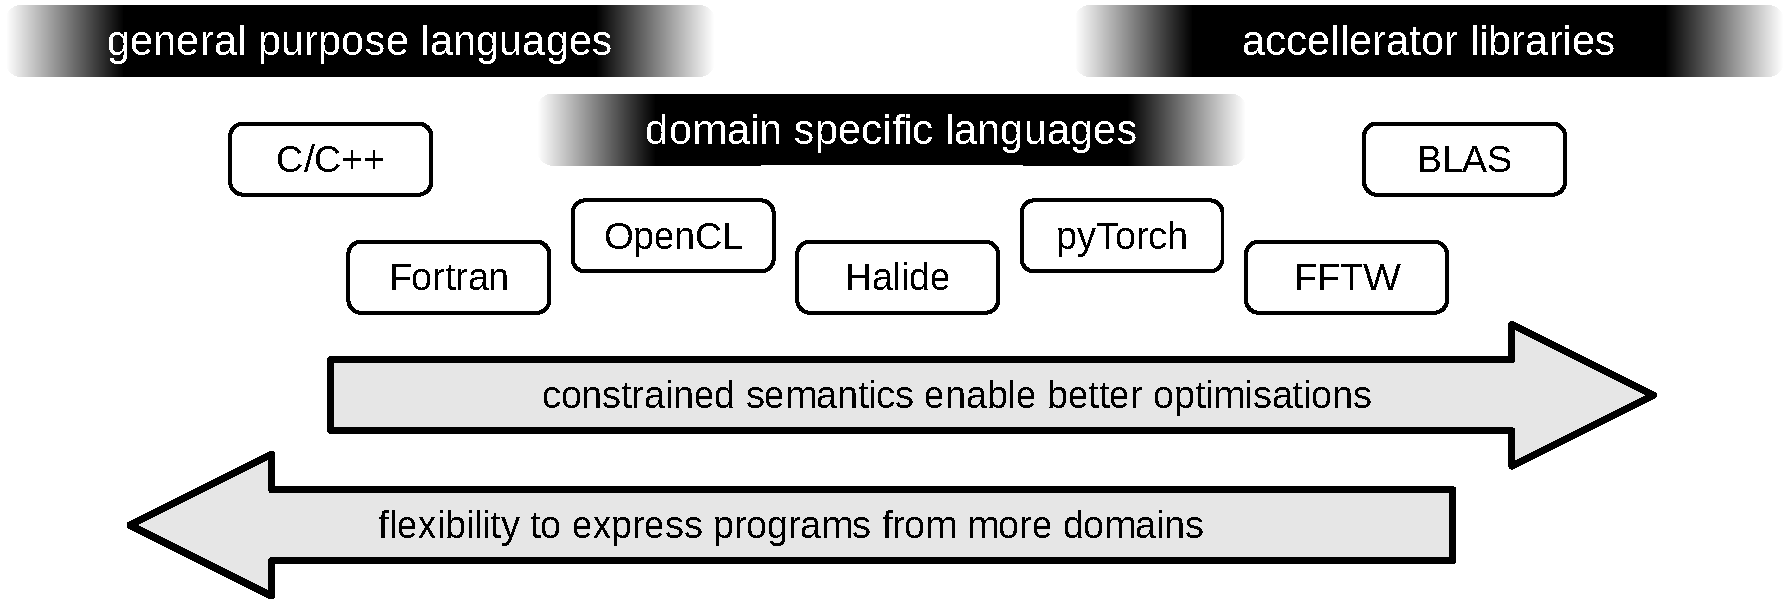
\includegraphics[width=\textwidth]{figures/DSLgradient}
\caption{Domain specific languages on a spectrum between general purpose
         languages and libraries.
         Decreasing flexibility allows for stronger reasoning and greater
         optimisation potential.}
\label{specialgradient}
\end{figure}

    In conclusion, the superior optimisation potential of libraries and
    domain-specific kernel compilers is a consequence of operating in more
    constrained conditions than host compilers.
    While expert programmers can often apply domain knowledge themselves
    when using versatile general-purpose languages, this potential can
    automatically be uncovered by specialised tools.
    The restrictions on input programs imply domain knowledge that is leveraged
    to make stronger assumptions, use more powerful models and generate better
    code.

    {\bf
    More restrictive program models result in additional optimisation
    opportunities and increased portability.
    Compilers use program models that correspond closely to their input
    programming languages.
    This correspondence could be decoupled by automatically recognising program
    parts that adhere to more constrained models, making the powerful
    domain-specific optimisation techniques of kernel compilers available to
    host compilers.
    }

\section{Moving on the Spectrum of Specialisation}

    To combine the positive aspects of both sides of the spectrum of
    specialisation, host compilers need methods to recognise more restrictive
    programming models within general-purpose code automatically.
    Reformulating the adhering program sections in domain-specific
    representations then makes the superior domain-specific reasoning from
    kernel compilers applicable also in the host compiler.

    Such an approach of detecting restricted models in general-purpose code has
    previously been used only for specific individual domains, and this involved
    extensive hand-implemented compiler analysis functionality.
    For example, the Polly compiler by \citet{Lengauer2012Polly} takes as
    input arbitrary C/C++ code and then recognises whether parts of this code
    are expressible in the more restrictive polyhedral model
    \citep{Karp:1967:OCU:321406.321418,benabderrahmane2010polyhedral}.
    The compiler then reformulates the relevant code in this system, which
    makes advanced optimisation techniques applicable that use the available
    domain knowledge of the restricted model for generating faster code
    \citep{Moll:2016:ISS:2892208.2892217,Doerfert2015Polly}, substantiating the
    hypotheses of \Cref{sec:hostkernel}.

\subsection{Contributions of this Thesis}

    This thesis derives a systematic approach for recognising constrained
    program sections during the compilation process that is not restricted to a
    particular model.
    The approach emerges from the analysis of a standard program model that host
    compilers use: Static Single Assignment (SSA) form intermediate
    representations.
    These SSA form representations are accessible to mathematical reasoning,
    with their most relevant features based on graph and list structures.
    With this in mind, structural restrictions on intermediate representation
    code -- corresponding to restricted, domain-specific models -- can be
    precisely formulated as mathematical constraints on a model of SSA form
    representations.
    The use of constraint solver techniques then makes automatic detection of
    adhering code regions feasible.

    Instead of manually implementing compiler analysis passes to recognise
    restricted models, a flexible constraint programming language is introduced,
    that can express many different such domain-specific models, and an
    accompanying toolchain is developed that uses these specifications to
    detect code sections that satisfy them automatically.
    This system captures the spectrum from \Cref{specialgradient}.
    On one extreme, sections of code are recognised as implementing
    specific algorithms, like matrix multiplications, that are merely
    parametrised with numbers.
    Next are algorithms that allow parametrisation with an operator.
    Stencil kernels, reduction operations or generalised histogram computations
    fall into this category.
    More generic again are programs that merely follow specific structural
    restrictions, such as code adhering to the polyhedral model.
    \Cref{chapter:candl,chapter:reductions,chapter:idioms} cover each of these
    domains, culminating in a system for the automatic heterogeneous
    acceleration of idiomatic code.

\section{Summary}

    The end of Moore's Law and Dennard Scaling has resulted in a shift away from
    homogeneous multi-processing, toward architectural innovation and
    specialised processor cores.
    The rising heterogeneity of computing resources poses a challenge to
    established compiler toolchains, which often only access the increasingly
    marginal homogeneous fraction of processing power.
    Therefore, programmers depend on domain-specific languages and libraries,
    which leverage domain knowledge from their restricted operating domains, to
    generate efficient code for this new hardware landscape.

    This domain knowledge can be made available to host compilers with
    approaches that automatically specialise general-purpose code and
    reformulate it in more restrictive program models.
    Previous work has established this on individual models, but this thesis
    develops a framework to formulate a wide range of restricted program models
    using a systematic approach based on constraint solving.
    To this purpose, a custom constraint programming language was developed
    and successively extended.
    Starting from a discussion of the underlying assumptions and features of
    Single Static Assignment code, the methodology is developed into a complete
    system, implemented as part of the mature Clang C/C++ compiler.

    In the later chapters, this core system is then applied in combination
    with other techniques in a range of different contexts.
    This includes the rapid prototyping of compiler optimisations, the
    automatic parallelisation of some program structures with indirect memory
    accesses, a new formulation of the polyhedral model and the detection of
    computational structures that cover important bottlenecks in typical
    scientific programs.

    Eventually, the techniques are combined into a fully integrated, extensible
    compiler tool for efficiently mapping sequential programs onto heterogeneous
    systems.
    This develops the thesis all the way from theoretical discussions of
    constraint programming approaches in compilers, to the experimental
    evaluation of real performance improvements on established benchmark suites
    and scientific applications.

\newpage
\section{Structure of the Thesis}

    This thesis is divided into six chapters.
    Following the introduction, the underlying methodology of this work is
    established in {\bf\Cref{chapter:theory}} and put in the context of
    conventional compiler analysis.
    Based on a model of Static Single Assignment (SSA) intermediate
    representations, the chapter derives a novel constraint programming approach
    to express algorithmic program structures as constraint formulas.
    Later sections of the chapter cover implementation decisions, algorithmic
    complexity, and a comparison to established Satisfiability Modulo Theory
    (SMT) problems.
    This forms the methodological basis for
    {\bf\Cref{chapter:candl,chapter:idioms,chapter:reductions}}.

    {\bf\Cref{chapter:literature}} gives a broad overview of the related work.
    This literature survey covers the four main areas of research in which this
    work is placed.
    Firstly, {\em constraint programming} underpins the methodology of this
    thesis.
    Secondly, {\em compiler analysis and auto-parallelisation} provide
    competing approaches against which the results in this thesis are evaluated.
    Thirdly, {\em heterogeneous computing} and the corresponding challenges
    motivate many of the compiler approaches that this research implements.
    Finally, ``{\em computational idiom}'' is an umbrella term for several
    overlapping concepts of algorithmic patterns that capture programming models
    in different positions on the spectrum of specialisation.

    {\bf\Cref{chapter:candl,chapter:idioms,chapter:reductions}}
    are each based on a published research article and elaborate on different
    applications of constraint programming in compilers.

    {\bf\Cref{chapter:candl}} develops a constraint programming language called
    CAnDL and presents an implementation in the LLVM compiler infrastructure.
    CAnDL that automatically generates compiler analysis passes from
    declarative specifications.
    The chapter explores several compiler analysis tasks with CAnDL,
    including the rapid implementation of peephole optimisations and the
    prototyping of graphics shader optimisations.
    This chapter is based on published research in
    \citet{Ginsbach:2018:CDS:3178372.3179515}.

    {\bf\Cref{chapter:reductions}} extends CAnDL into the Idiom Detection
    Langauge (IDL) and develops an auto-parallelising compiler for
    complex reduction and histogram computations built on IDL-powered analysis
    functionality.
    These computations cover many loops with indirect data access that are
    inaccessible to established approaches based on data flow and polyhedral
    analysis.
    The flexibility of constraint programming allows it to still capture such
    irregular computations.
    This chapter is based on published research in
    \citet{ginsbach2017discovery}.

    {\bf\Cref{chapter:idioms}} applies IDL to the detection of algorithmic
    structures that go beyond the scope of traditional compiler analysis:
    stencils, complex reductions and histograms, as well as sparse and dense
    forms of linear algebra.
    The detection in LLVM enables the automatic heterogeneous
    acceleration of sequential code and result in significant speedups on
    established benchmark suites.
    This chapter is based on published research in
    \citet{Ginsbach:2018:AML:3173162.3173182}.


\chapter{Literature Survey}
    \label{chapter:literature}
    
    The research contributions of this thesis are based on a novel constraint
    programming approach on compiler intermediate representation.
    This chapter introduces the theoretical underpinnings of this approach,
    based on a mathematical model of static single assignment form (SSA).
    With the help of this model, concepts that are typically discussed on a
    programming language level are transferred onto the structurally simple,
    yet semtantically expressive class of SSA compiler intermediate
    representations.

    Constraint formulas on SSA respresentations initially appear to mimic
    pattern matching approaches on abstract syntax tree (AST) level.
    However, they quickly prove themselves to be vastly more expressive.
    Some consideration is necessary to handle search space explosion, but
    the reward are much more powerful recognition capabilities and the
    expression of higher level algorithmic structures, which are impossible to
    define syntactically on programming language level.
    Later chapters will explore the power of this approach in detail, by
    building a complete constraint programming language on top of the theory in
    this chapter, and by then using it to solve real compiler analysis problems.

    After defining a mathematical foundation of SSA form and introducing
    formalisms for the expression of basic contraint problems on top of it,
    several standard definitions from compiler theory are reformulated in the
    framework.
    This includes common graph properties, including the concept of domination,
    as well as control flow structures such as single entry single exit blocks.
    All of this lays the foundations for the succeeding chapter.

    Finally, for the practical application of constraint programming to compiler
    intermediate representation, efficient solver techniques are needed.
    The last section in this chapter discusses strategies for limiting
    compile time explosion and explores analogies of the described model to
    standard Satisfiability Modulo Theory (SMT) problems.
    This gives further insights into performance improvements and puts the
    work into a broader theoretical context.

\section{Introduction}

    Modern compilers for procedural languages such as
    C/C++, Fortran or JavaScript typically use a succession of different
    representations for the program during compilation.
    They can be grouped into categories and reflect the requirements of
    the compilation stages they are used in.
    \linebreak
    {\bf Front end representations} are close to the source program and
    naturally reflect the internals of the compiler front end, especially the
    parser.
    Typically, they are built on an abstract syntax tree representation with
    additional annotations, such as type information.
    In addition to encoding program logic, these representations are rich in
    information about syntactic and  stylistic choices of the programmer.
    They scale in complexity with the source language and further obscure the
    program semantics by not resolving complex language features, such as
    operator overloading.
    \linebreak
    {\bf Back end representations} are based on a model of the target hardware.
    These representations typically approach an assembly style format,
    exposing specific instruction set architectures of the hardware.
    Back end representations are concerned with problems that are removed from
    the algorithmic core of the user program, such as register allocation and
    instruction scheduling.
    \\
    {\bf Static Single Assignment} (SSA) form has emerged as a suitable
    representation in the middle end, which is traditionally responsible for
    applying complex optimising transformations.
    SSA abstracts away the complexities of both the source language and the
    target architecture, instead focusing on a relatively simple semantic
    description of the user program that enables reliable analysis and platform
    independent reasoning.
    It is these properties that also make it the natural representation for
    expressing algorithmic structures.

    Static Single Assignment is not a strictly defined or mathematically
    codified standard, but instead refers to a group of representations that
    share important characteristics,
    the eponymous SSA property being only one among them.
    Instruction sets, syntax and type systems of the different
    SSA intermediate representations vary considerably, depending on the
    requirements of the source languages (static or dynamic)
    and the operating constraints (just-in-time or ahead-of-time).
    Some prominent examples of compilers that utilize SSA for their
    optimisation passes include {\bf clang} (LLVM IR), {\bf gcc} (GIMPLE),
    {\bf v8 Crankshaft} (Hydrogen) and {\bf SpiderMonkey} (IonMonkey/MIR).
    Despite many differences, they share the same fundamental paradigms
    and many of the differences can be abstracted away as implementation
    specific details.

    Fundamentally, a program in single static assignment form is made up of
    functions, which are represented as sequences of instructions, grouped into
    basic blocks and operating on virtual registers.
    The control flow is handled via jump instructions at end of basic blocks.
    The virtual registers, within a function, can be assigned only at a single
    static location each, which has very useful implications as we will later
    see.
    As opposed to syntax-heavy representations, SSA form is a searialized
    program representation, where expressions have been turned into lists of
    instructions and control flow structures into lists of basic blocks.
    The following sections explore how this serial nature makes constraint
    programming concepts naturally applicable.

\subsection{Static Single Assignment Form}

\begin{figure}[t]
\centering
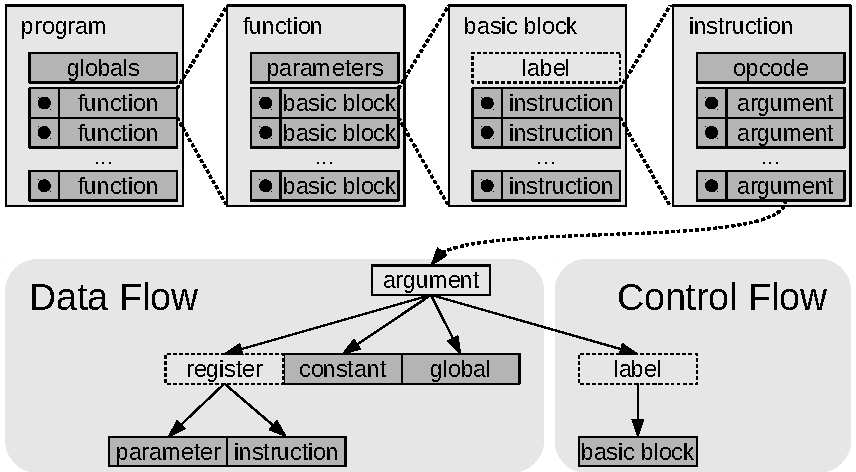
\includegraphics{figures/ssaoverview}
\caption{Structural overview of SSA: Programs are represented as hierarchies of
    lists. The SSA property makes registers implicit, values can be statically
    matched to defining instructions.}
\label{fig:ssaoverview}
\end{figure}

    SSA representations of programs are highly serialised, as shown in
    \autoref{fig:ssaoverview}:
    Programs are lists of functions, functions are lists of basic blocks,
    basic blocks are lists of instructions and instructions are most
    fundamentally lists of arguments.

    The individual instructions operate on an abstract machine, which provides
    an unlimited number of identical registers and a well defined instruction
    set.
    The control flow is expressed as branch instructions, which direct the
    execution conditionally or unconditionally to other basic blocks.
    Basic blocks may have labels or be identified simply by enumerating them.
    Instruction arguments can be registers, constants or globals and branch
    instructions additionally take basic block labels.
    Instructions can write their result into a single output register.
    Branch instructions always terminate a basic block, control flow divergence
    within basic blocks is not possible.

    The static single assignment property stipulates that within a function,
    no register can be written at more than a single static location.
    This makes the data dependencies between the instructions explicit, as it
    implies that registers can be identified directly with the instructions that
    write to them.
    The registers themselves can therefore be considered implicit, with only the
    data flow between instructions required to recover them.

    In the presence of dynamic control flow behaviour in the program, most
    simply in the case of a conditional branch, it is evidently not possible to
    match values to producing instructions statically.
    This is resolved with {\em phi} instructions.
    These instructions select a value from several arguments depending on the
    previously executed basic block, i.e.\ depending on the branch from where
    the execution reached the basic block containing the phi node.

\subsection{Example of Static Single Assignment Form}

    \autoref{ssaexample} shows many of the key features of static single
    assignment form and how they naturally emerge from simplification steps of
    the source code of procedural languages.
    This is demonstrated on an example function ``{\tt sqrt}'' written in C,
    which  appriximates the square root of a value iteratively using the
    Babylonian method as described in \autoref{babylonian_equation}.

\begin{equation}
    x_0\approx\sqrt{S},\text{\hspace{1cm}}
    x_{n+1}=\frac{x_n+\frac{S}{x_n}}{2}\text{\hspace{1cm}}
    \implies\text{\hspace{1cm}}
    \lim_{n\rightarrow\infty}x_n=\sqrt{S}
    \label{babylonian_equation}
\end{equation}

    Starting from the source code {\bf a)} at the top left of the figure, the
    function is first simplified by breaking down complex expressions as far as
    possible.
    This results in a sequentialisation of the expressions into their
    most basic operations, shown at the top right {\bf b)}, introducing
    explicit variables that store the previously implicit temporary values.
    This greatly simplifies and normalises the program, with many of the
    remaining simple expressions directly mapping to individual processor
    instructions.

    In a second step, the structured control flow of the program is replaced
    with goto statements that coordinate the control between basic blocks.
    This is shown at the bottom right {\bf c)}.
    While this does not ease the intuitive understanding of the program, it
    unifies the many control flow structures provided in the source language
    into a single mechanism.
    This makes automatic analysis of the program a less complex task.
    Importantly, no relevant information is lost by discarding the control flow
    structures.
    They can be reconstructed algorithmically.

    Lastly, the static single assignment property is introduced.
    Any variable that is assigned in more than one static place in the program
    is instead duplicated into multiple variables.
    Where necessary, these now distinct variables are bound together with
    $\Phi$ nodes.
    This cannot be directly expressed in the C syntax {\bf d)} at the bottom
    left.
    Instead, the behaviour is documented by comments in lines 8-13.
    The impact of the static single assignment property change seems minor
    at first, but it has convenient implications.
    As all local variables are written exactly once, the distinction between
    their declarations and definitions becomes obsolete.
    This furthermore implies that it is always known statically, which
    expression yielded the value of each variable.
    Variable names become identifiers of the expressions themselves.
    This makes many optimising transformation strainghtforward to implement.
    As a trivial example, it immediately guarantees that the variable $i$ in the
    example always has the value zero.

    With an understanding of how SSA form emerges during compilation, it is now
    the aim to use the serialised nature of it to contruct a convenient
    mathematical model.
    The crucial observation is that most items in SSA form functions can be
    easily enumerated and identified by their index.
    This includes the function parameters, expressions and variables.
    This means that properties of SSA form functions can be described using
    integers, making for a convenient and easy mathematical language.

\begin{figure}[p]
    \begin{minipage}{0.48\textwidth}
\begin{lstlisting}[language=C,captionpos=t,title=
   {{\bf(a)} {} C source function:\leftskip=0pt}]
double sqrt(double S) {
  double x = 1.0;
  for(int i=0; i<N; i+=1)
    x = 0.5 * (x + S / x);
  return x;
}
\end{lstlisting}
\begin{lstlisting}[language=C,captionpos=t,title=
   {{\bf(d)} {} The SSA property is introduced:\leftskip=0pt}]
double sqrt(double S) {
entry:
  double x = 1.0;
  int i = 0;
  goto header;

header:
  int i2 = /* if reached
    from line  5: i,
    from line 23: i3 */
  int x2 = /* if reached
    from line  5: x,
    from line 23: x3 */
  bool test = i2 < N;
  if(test) goto loop;
      else goto exit;

loop:
  double t1 = S / x2;
  double t2 = x2 + t1;
  double x3 = 0.5 * t2;
  int i3 = i2+1;
  goto header;

exit:
    return x2;
}
\end{lstlisting}
\end{minipage}
\hfill
\begin{minipage}{0.48\textwidth}
\begin{lstlisting}[language=C,basicstyle=\linespread{1.06451612903}\ttfamily,
                   captionpos=t,title=
   {{\bf(b)} {} Complex expressions are broken down:\leftskip=0pt}]
double sqrt(double S) {
  double x = 1.0;
  for(int i=0; i<N; i+=1)
  {
    double t1 = S / x;
    double t2 = x + t1;
    x = 0.5 * t2;
  }
  return x;
}
\end{lstlisting}
\begin{lstlisting}[language=C,basicstyle=\linespread{1.06451612903}\ttfamily,
                   captionpos=t,title=
   {{\bf(c)} {} Structured control flow is expanded:\leftskip=0pt}]
double sqrt(double S) {
entry:
  double x = 1.0;
  int i = 0;
  goto header;

header:
  bool test = i < N;
  if(test) goto loop;
      else goto exit;

loop:
  double t1 = S / x;
  double t2 = x + t1;
  x = 0.5 * t2;
  i = i+1;
  goto header;

exit:
    return x;
}
\end{lstlisting}
\end{minipage}

    \caption{Static Single Assignment emerges from successive simplification
             and normalisation of source language features: 
             Demonstration on an example C function that approximates the
             square root of an input value with the Babylonian method.
             The transformation results {\bf b)-d)} are redered in C.
             Real compilers typically operate on
             dedicated internal representations instead.}
    \label{ssaexample}
\end{figure}

\newpage
\section{Deriving a Mathematical Model for SSA}

    In order to develop constraint programming on real world SSA programs with
    mathematical rigour, a sound model is needed first.
    The aim here is not to introduce an operational semantics, or more
    generally to derive a model for the execution of SSA programs.
    Instead, the section will investigate the static structure, focusing on
    clear notation of the commonalities of existing SSA intermediate
    representations.
    This requires naming conventions for some of the basic features of
    SSA programs.
    The remainder of this section adheres to \autoref{not:ssa} when referring to
    these features.
    No specific representative of the class of SSA representations is chosen
    here.

\begin{figure}[h]
\begin{notation}{Static Single Assignment Function}{ssa}
    For the remainder of this section, some function $\mathcal F$ in SSA form is
    assumed fixed. 
    The following identifiers are then used to describe the features of this
    function.

    \begin{itemize}
    \item $n_p$ is the number of function parameters $par_1,\dots par_{n_p}$.
    \item $n_i$ is the number of instructions $ins_1,\dots ins_{n_i}$ in the
          function, ordered depth first, starting from the execution entry.
    \item $n_g$ is the number of unique globals $glb_1,\dots glb_{n_g}$ that are
          referenced as an operand of any of the instructions.
    \item $n_c$ is the number of unique constants $cst_1,\dots cst_{n_g}$ that
          are referenced as an operand of any of the instructions.
    \end{itemize}
\end{notation}
\end{figure}

    This notation fixes several decisions about the utilised model.
    Firstly, the model captures only a single function.
    Secondly, basic block structures are not explicitly encoded.
    Instead, all instructions of the function are listed sequentially in depth
    first order, starting from the function entry.
    Basic blocks can be reconstructed from the control flow, as discussed later.
    Thirdly, the argument structure of the instructions is not represented and
    will instead be modeled separately.

\subsection{Data Flow and Control Flow}

    The data flow between interaction as well as the control flow is captured in
    graph structures.
    The static single assignment property makes registers implicit, therefore
    the direct interaction between instructions becomes the natural model for
    data flow.
    Instruction arguments fall into four categories: function parameters,
    constants, globals and other instructions.
    Branching instructions also take basic block labels as branch targets,
    but they can be treated separately in the control flow graph that is
    introduced later.
    All instruction arguments are therefore taken from the named sets introduced
    in \autoref{not:ssa}.

    For each function, these sets can be statically determined and are finite.
    Therefore, a single integer is enough to encode each instruction argument as
    an index into the union of those four sets.
    Together with the list based representation, this allows for the
    entire argument structure of the instructions in an SSA function to be
    conveniently turned into a labelled multigraph, with edge labels accounting
    for the positional order of the arguments.
    These observations lead to the definition of the set of used values in
    \autoref{def:usedvalues} and the data flow graph in \autoref{def:dfg}.

\begin{figure}[h]
\begin{definition}{Set of Used Values}{usedvalues}
    The {\em set of used values} of the SSA function $\mathcal F$ is the tuple
    \begin{align*}
       val_1,\dots,val_{n_{pigc}} := par_1,\dots par_{n_p},
                                     ins_1,\dots ins_{n_i},
                                     glb_1,\dots glb_{n_g},
                                     cst_1,\dots cst_{n_g}.
    \end{align*}
    The value $n_{pigc}:=n_p+n_i+n_g+n_c$ is the {\em number of used values}.
\end{definition}

\begin{definition}{Data Flow Graph}{dfg}
    The {\em data flow graph} of the SSA function $\mathcal F$ is the set
    $DGF_{\mathcal F}\subset \mathbb N^3$ such that
    \begin{align*}
        (a,b,n)\in DFG_{\mathcal F}\iff 1\leq a\leq n_{pigc}
            \mathrel{\land}(val_a\text{ is the $n$th argument of }ins_b).
    \end{align*}
\end{definition}
\end{figure}

    Complementing the data flow graph is the control flow graph of the function,
    as introduced in \autoref{def:cfg}.
    The control flow graph is usually defined on a basic block granularity, but
    here it will be defined directly on instructions, in order to better
    complement the data flow graph.
    The basic block structure is easily recoverable from this representations.

\begin{figure}[h]
\begin{definition}{Control Flow Graph}{cfg}
    The {\em control flow graph} of the SSA function $\mathcal F$ is the set
    $CGF_{\mathcal F}\subset \mathbb N^3$ such that
    \begin{align*}
        (a,b,n)&{}\in CFG_{\mathcal F}\iff n_p<a,b\leq n_p+n_i\mathrel{\land}\\
               &\left(\begin{aligned}[c]
                                    (\neg (ins_{a-n_p}\text{ terminates basic block})\mathrel{\land}{}&b=a+1\mathrel{\land}n=1)\\
                      \mathrel{\lor}(\phantom{\neg}(ins_{a-n_p}\text{ terminates basic block})\mathrel{\land}{}&ins_{b-n_p}\text{ first instruction in}\text{ $n$th}\\[-0.5em]
                                                   &\text{target basic block of }ins_{a-n_p})
        \end{aligned}\right).
    \end{align*}
\end{definition}
\end{figure}

    The control flow graph in \autoref{def:cfg} is peculiar in its omission of
    basic block structures.
    This is visible in the definition, where edges are of two distinct types:
    They are either an edge within a basic block, or they are an edge between
    the terminator of one basic block and the initial instruction in an another.
    This apparent loss of information is not substantial, the basic blocks can
    be reconstructed.
    However, it has implications for modeling $\Phi$ nodes.
    They are modeled as instructions, with their value depending on the last
    executed jump instruction.

\subsection{Identifying Remaining Structure}

    With the control flow and data flow separated into distinct mathematical
    structures, individual instructions are encoded by their opcodes alone.
    This is demonstrated in \autoref{fig:separation}.
    At the top of the figure is a simple function in an abstract SSA
    representation.
    It calculates an approximation of the square root of a number using the
    Babylonian method, as previously introduced in \autoref{ssaexample}.
    The function has 11 instructions separated into 4 basic blocks, with the
    majority of the instructions in a loop structure that iteratively improves
    the result.

    The entire semantic information that is encoded in this SSA representation
    can be recovered from the structures at the bottom of the figure:
    per-instruction opcode information, lists of the parameters, constants and
    globals used, the data flow graph as in \autoref{def:dfg} and the control
    flow graph as in \autoref{def:cfg}.
    The information at the bottom left will be further discussed later.
    It may involve a type system and also the instruction set remains to be
    specified.

    In order to demonstrate the equivalence in \autoref{fig:separation},
    consider these reconstruction steps:
\begin{enumerate}
    \item The basic block boundaries are reconstructed by identifying all
          consecutive instructions $A$, $B$ where at least one of the
    conditions hold:
    \begin{itemize}
        \item $A$ does not have exactly one outgoing edge to $B$ or
        \item $B$ does not have exactly one incoming edge from $A$.
    \end{itemize}
    \item Basic block labels and register names can be chosen arbitrarily.
    \item The arguments of all operations can be immediately filled in with the 
          DFG. Similarly, the CFG directly provides the target instructions
          for goto statements.
    \item Incoming edges of $\Phi$ nodes are matched with incoming values using
          the convention that the incoming values are ordered (with respect to
          their labels in the data flow graph) according to the position of the
          incoming basic blocks in the list of instructions.
\end{enumerate}

\begin{figure}[b]
\begin{definition}{Instruction Set and Type System}{isatypes}
    For a specific member $m$ of the family of SSA representations, there is
    a set of opcodes $Opcodes_m$ and a set of types $Types_m$.
\end{definition}
\end{figure}

    The only part of the SSA representation that still needs to be modeled is
    the per-value information at the bottom left of \autoref{fig:separation},
    which in this case is nothing more than a list of opcodes, and the list of
    constants, paramters and globals.
    The opcodes are specific to different SSA representations, although a wide
    overlap exists (basic arithmetic, phi nodes).
    This chapter aims to capture commonalities of SSA representations, the study
    of instruction sets and type systems is orthogonal to this.
    Therefore, these structures remain opaque at this point and are modeled as
    arbitrary sets as in \autoref{def:isatypes}.

\begin{figure}[p]
\centering
\begin{minipage}{0.42\textwidth}
\begin{tabular}{|cl|}
\multicolumn{2}{c}{{\bf function} Sqrt($S$)}\\
\hline
{\bf entry} & $\text{goto } header$\\
\hline
\multirow{4}{*}{\bf header} & $i \leftarrow \Phi(entry:0,loop:i')$\\
                            & $x \leftarrow \Phi(entry:1,loop:x')$\\
                            & $c \leftarrow i<N$\\
                            & $\text{if }c\text{ goto }loop\text{ else }exit$\\
\hline
\multirow{5}{*}{\bf loop} & $t_1\leftarrow S/x$\\
                          & $t_2\leftarrow x+t_1$\\
                          & $x'\leftarrow t_2/2$\\
                          & $i'\leftarrow i+1$\\
                          & $\text{goto }header$\\
\hline
{\bf exit} & $\text{return }x$\\
\hline
\end{tabular}
\end{minipage}

\vspace{3.2mm}
{\huge
$\cong$}
\vspace{3.2mm}

$\left(
\begin{minipage}{5.5cm}
\centering
\hspace{-2em}
\begin{tabular}{r}
\phantom{00}\\
1:
\end{tabular}
\begin{tabular}{|l|}
\multicolumn{1}{p{3cm}}{{\bf parameters:}}\\
\hline
$S$\\
\hline
\end{tabular}\\
\hspace{-2em}
\begin{tabular}{r}
\phantom{88}\\
2:\\
3:\\
4:\\
5:\\
6:\\
7:\\
8:\\
9:\\
10:\\
11:\\
12:
\end{tabular}
\begin{tabular}{|l|}
\multicolumn{1}{p{3cm}}{{\bf instructions:}}\\
\hline
$\text{goto } \square$\\
$\Phi(\square:\square,\square:\square)$\\
$\Phi(\square:\square,\square:\square)$\\
$\square<\square$\\
$\text{if }\square\text{ goto }\square\text{ else }\square$\\
$\square/\square$\\
$\square+\square$\\
$\square/\square$\\
$\square+\square$\\
$\text{goto } \square$\\
$\text{return }\square$\\
\hline
\end{tabular}\\
\hspace{-2em}
\begin{tabular}{r}
\phantom{88}\\
13:
\end{tabular}
\begin{tabular}{|l|}
\multicolumn{1}{p{3cm}}{{\bf globals:}}\\
\hline
$N$\\
\hline
\end{tabular}\\
\hspace{-2em}
\begin{tabular}{r}
\phantom{88}\\
14:\\
15:\\
16:
\end{tabular}
\begin{tabular}{|l|}
\multicolumn{1}{p{3cm}}{{\bf constants:}}\\
\hline
$1$\\
$2$\\
$0$\\
\hline
\end{tabular}
\end{minipage}
\right)\hspace{1em}\text{\huge +}\hspace{1em}\left(
\begin{minipage}{5.5cm}
\centering
\setlength{\abovedisplayskip}{0pt}
\setlength{\belowdisplayskip}{0pt}
\vspace{-0.5em}
\begin{align*}
DFG_\mathcal F=\{
&10\xrightarrow{2}3,\ 16\xrightarrow{1}3,\\[-0.153em]
&9\xrightarrow{2}4,\ 14\xrightarrow{1}4,\\[-0.153em]
&3\xrightarrow{1}5,\ 13\xrightarrow{2}5,\\[-0.153em]
&5\xrightarrow{1}6\\[-0.153em]
&1\xrightarrow{1}7,\ 4\xrightarrow{2}7,\\[-0.153em]
&4\xrightarrow{1}8,\ 7\xrightarrow{2}8\\[-0.153em]
&8\xrightarrow{1}9,\ 15\xrightarrow{2}9\\[-0.153em]
&3\xrightarrow{1}10,\ 14\xrightarrow{2}10,\\[-0.153em]
&4\xrightarrow{1}12\}\\
CFG_\mathcal F=\{
&2\xrightarrow{1}3,\\[-0.153em]
&3\xrightarrow{1}4,\\[-0.153em]
&4\xrightarrow{1}5,\\[-0.153em]
&5\xrightarrow{1}6,\\[-0.153em]
&6\xrightarrow{1}7,\ 6\xrightarrow{2}12,\\[-0.153em]
&7\xrightarrow{1}8,\\[-0.153em]
&8\xrightarrow{1}9,\\[-0.153em]
&9\xrightarrow{1}10,\\[-0.153em]
&10\xrightarrow{1}11,\\[-0.153em]
&11\xrightarrow{1}3\}
\end{align*}
\end{minipage}
\right)$

\caption{SSA representation is decomposed into individual instructions, data
         flow and control flow.
         This is an equivalent representation of the function, no semantic
         information is lost.
         The example is a rendering of the Babylonian method in
         \autoref{ssaexample}, abstracting away the C syntax.}
\label{fig:separation}
\end{figure}

\subsection{Putting the Model Together}

\begin{figure}[p]
    \begin{definition}{Mathematical Model of SSA programs}{ssamodel}
    The {\em SSA model} of the function $\mathcal F$ is the tuple
    \begin{align*}
        (DFG_\mathcal{F},
         CFG_\mathcal{F},
         T_\mathcal{F},
         P_\mathcal{F},
         I_\mathcal{F},
         G_\mathcal{F},
         C_\mathcal{F}),
    \end{align*}
    where

    \begin{itemize}
    \item $DFG_\mathcal{F}\subset\mathbb N^3$ and
          $CFG_\mathcal{F}\subset\mathbb N^3$ are the data flow and control
          flow graph.
    \item $T_\mathcal F\subset\mathbb N\times Types$ is the type model, defined
          by the property
          \begin{align*}
              (k,ty)\in T_\mathcal F\iff 1\leq k\leq n_{pigc}
                  \mathrel{\land}(val_k\text{ has type }ty).
          \end{align*}
    \item $P_\mathcal F\subset\mathbb N$ and $G_\mathcal F\subset\mathbb N$
          are the parameter model and global model, defined by the properties
          \begin{align*}
              k\in P_\mathcal F\iff& 1\leq k\leq n_p\text{ and}\\
              k\in G_\mathcal F\iff& n_p+n_i<k\leq n_p+n_i+n_g.
          \end{align*}
    \item $I_\mathcal F\subset\mathbb N\times Opcodes$ is the instruction model,
          defined by the property
          \begin{align*}
              (k,op)\in I_\mathcal F\iff n_p<k\leq n_p+n_i
                  \mathrel{\land}(ins_{k-n_p}\text{ has opcode }op).
          \end{align*}
    \item $C_\mathcal F\subset\mathbb N\times\mathbb R$ is the constant model,
          defined by the property
          \begin{align*}
              (k,x)\in C_\mathcal F\iff{}&n_p+n_i+n_g<k\leq n_{pigc}\\
                        \mathrel{\land}{}&(cst_{k-n_p-n_i-n_g}
                        \text{ has numeric value equal to }x).
          \end{align*}
    \end{itemize}
\end{definition}

\begin{notation}{Graph Projections}{convenience}
    For $G\subset\mathbb N^3, k\in\mathbb N$, the following notation applies:
    \begin{align*}
        G^k:=&\{(a,b)\in\mathbb N^2\mid (a,b,k)\in G\}\\
        G^*:=&\{(a,b)\in\mathbb N^2\mid \exists c\in\mathbb N:(a,b,c)\in G\}.
    \end{align*}

    For $G\subset\mathbb N\times\mathbb R, c\in\mathbb R$, the following
    notation applies:
    \begin{align*}
        G^c:=&\{a\in\mathbb N\mid (a,c)\in G\}\\
        G^*:=&\{a\in\mathbb N\mid \exists c\in\mathbb R:(a,c)\in G\}.
    \end{align*}
\end{notation}
\end{figure}

    With separate mathematical models in place for all the individual structures
    that interact in SSA representations, it is now possible to compile a
    complete model.
    \autoref{def:ssamodel} shows this completed model.
    The data flow graph and control flow graph were discussed in detail
    previously, but some clarifications are required for the remaining
    structures.

    The instruction model, type model and constant model all conceptually assign
    additional information from different domains to the used values in the
    program.
    It would be perhaps more intuitive at first to model them as functions
    instead, with $I_\mathcal F\colon\mathbb N\rightarrow Opcode$,
    $T_\mathcal F\colon\mathbb N\rightarrow Types$,
    $C_\mathcal F\colon\mathbb N\rightarrow \mathbb R$.
    The model in \autoref{def:ssamodel} has several advantages over such an
    approach.
    Firstly, it makes it easy to account for what would be partial function
    definitions, e.g.\ only instructions have opcodes.
    Secondly, it can express type hierarchies and instruction categories.
    For example, a value might be a ``pointer'' and an ``integer pointer'' at
    at the same time.
    The same holds for opcodes, where an instruction might be an ``arithmetic''
    operation and in particular a ``subtraction'' at the same time.
    Thirdly, the representation as a set makes the encoding in appropriate data
    structures more intuitive and will help in later sections.

    Finally, the parameter model and global model are essentially encoding
    boolean predicates on values.
    The models simply mark all the used values that are parameters or globals.
    They can therefore only be distinguished and identified by their position
    in the list of values.
    This is clearly sufficient for parameters, as they are distinguished by
    their positionality.
    However, from a program-wide perspective, global variable names arguably
    carry significance.
    However, the model operates per function, as previously said.

\subsection{Graph Projections}

    Additional notation is introduced in \autoref{not:convenience} for
    convenience.
    The representation of data flow and control flow as labeled multigraphs
    often contains more information than required.
    The presented graph projection allow different ways of reducing the
    dimensionality of the model structures that will be useful in later
    sections.

    The control flow and data flow graph can be simplified by either filtering
    for specific edge labels or by discarding them entirely.
    For example, the graph $DFG_\mathcal F^*$ has erased all the information
    about instruction operand order.
    Similarly, the graph $CFG_\mathcal F^1$ has filtered the control flow to
    only consider the first edge at any branch.

    Similar notation is used to simplify the instruction, type and constant
    models.
    For example, $C_\mathcal F^*$ discards the value information and gives a
    simple poolean predicate, akin to the global and parameter model.
    On the other hand $C_\mathcal F^0$ contains all the zero-valued constants.

    These different simplifications will enable the easier formulation of
    constraint programs later.

\subsection{Application to LLVM}

    The previously introduced mathematical model of SSA programs is independent
    of the chosen SSA representation.
    However, the specialisation to concrete compiler problems is the aim of this
    work.
    Arguably the most prevalent SSA compiler intermediate representation is
    LLVM IR, therefore it will be the main vessel for demonstration in this
    thesis.

    LLVM is a compiler infrastructure built around a central intermediate
    representation LLVM IR.
    The name was originally an acronym for ``Low Level Virtual Machine'',
    conceptualising the intermediate representation as a typed assembly style
    language of a virtual machine.
    The instruction set is vaguely aligned to C semantics, however the project
    has matured beyond this background.
    It is now a widely influential framework, front ends exist for a diverse set
    of langauges including C/C++, Haskell, Julia, Objective-C, Rust, Scala and
    CUDA.

    Other mainstream compilers, particularly the gcc project, in effect utilise
    very similar representations internally.
    However, LLVM is unique in its insistence n LLVM IR being a well documented
    language, as opposed to an obscure internal abstraction.
    This makes it uniquely suitable for research implementations.
    While the theory of this work is developed independenyly from LLVM and
    applies in general, LLVM will the the language of choice for all
    implementations.
    Therefore, a detailed example is required.


\begin{figure}[p]
\paragraph*{a)} C source code of a {\tt dot} product function implementation
\begin{lstlisting}[language=C]
double dot(double* a, double *b, size_t n)
{
  double d = 0.0;
  for(int i = 0; i < n; i++)
    d += a[i]*b[i];
  return d;
}
\end{lstlisting}

\paragraph*{b)} LLVM IR representation of the same {\tt dot} product function
\begin{lstlisting}[language=LLVM]
define double @dot(double* %0, double* %1, i64 %2) {
; <label>:3:
  %4 = icmp eq i64 %2, 0
  br i1 %4, label %5, label %7

; <label>:5:
  %6 = phi double [ 0.0, %3 ], [ %16, %8 ]
  ret double %6

; <label>:7:
  br label %8

; <label>:8:
  %9 = phi i64 [ %17, %8 ], [ 0, %7 ]
  %10 = phi double [ %16, %8 ], [ 0.0, %7 ]
  %11 = getelementptr double, double* %0, i64 %9
  %12 = load double, double* %11
  %13 = getelementptr double, double* %1, i64 %9
  %14 = load double, double* %13
  %15 = fmul double %12, %14
  %16 = fadd double %10, %15
  %17 = add i64 %9, 1
  %18 = icmp eq i64 %17, %2
  br i1 %18, label %5, label %8
}
\end{lstlisting}
\caption{The correspondence between C and LLVM IR on an example function.
         The function computes the dot product of two vectors in a simple
         reduction loop.
         In the LLVM IR -- generated by clang -- pointer calculations and memory
         accesses are visible within the SSA representation.}
\label{llvmirexample}
\end{figure}

\newpage

    \autoref{fig:derivemaths} shows in detail how the SSA model is derived from
    the LLVM IR representation of the program in \autoref{llvmirexample}.
    In the top left, implementations of the dot product function are shown
    in three programming languages that LLVM supports: Fortran, C and C++.
    On the top right is the corresponding LLVM IR code.
    While this will not be precisely identical for the different
    implementations, the basic structure of it is independent of source
    language.

    In the middle row, the information from the the SSA representation is split
    into three components:
    Labeled multigraphs for the data flow and control flow, as well as
    the per-instruction properties as a list.
    This constains all semantically relevant information of the program, as was
    demonstrated previously.
    In the bottom row, the mathematical representation of the function is shown,
    adhering to \autoref{def:ssamodel}.
    The labeled multigraphs for the control flow and data flow graphs are
    represented as sets of $3$-tuples of integers.

\begin{figure}[p]
\centering
\begin{blackbox}{Textual Representation}
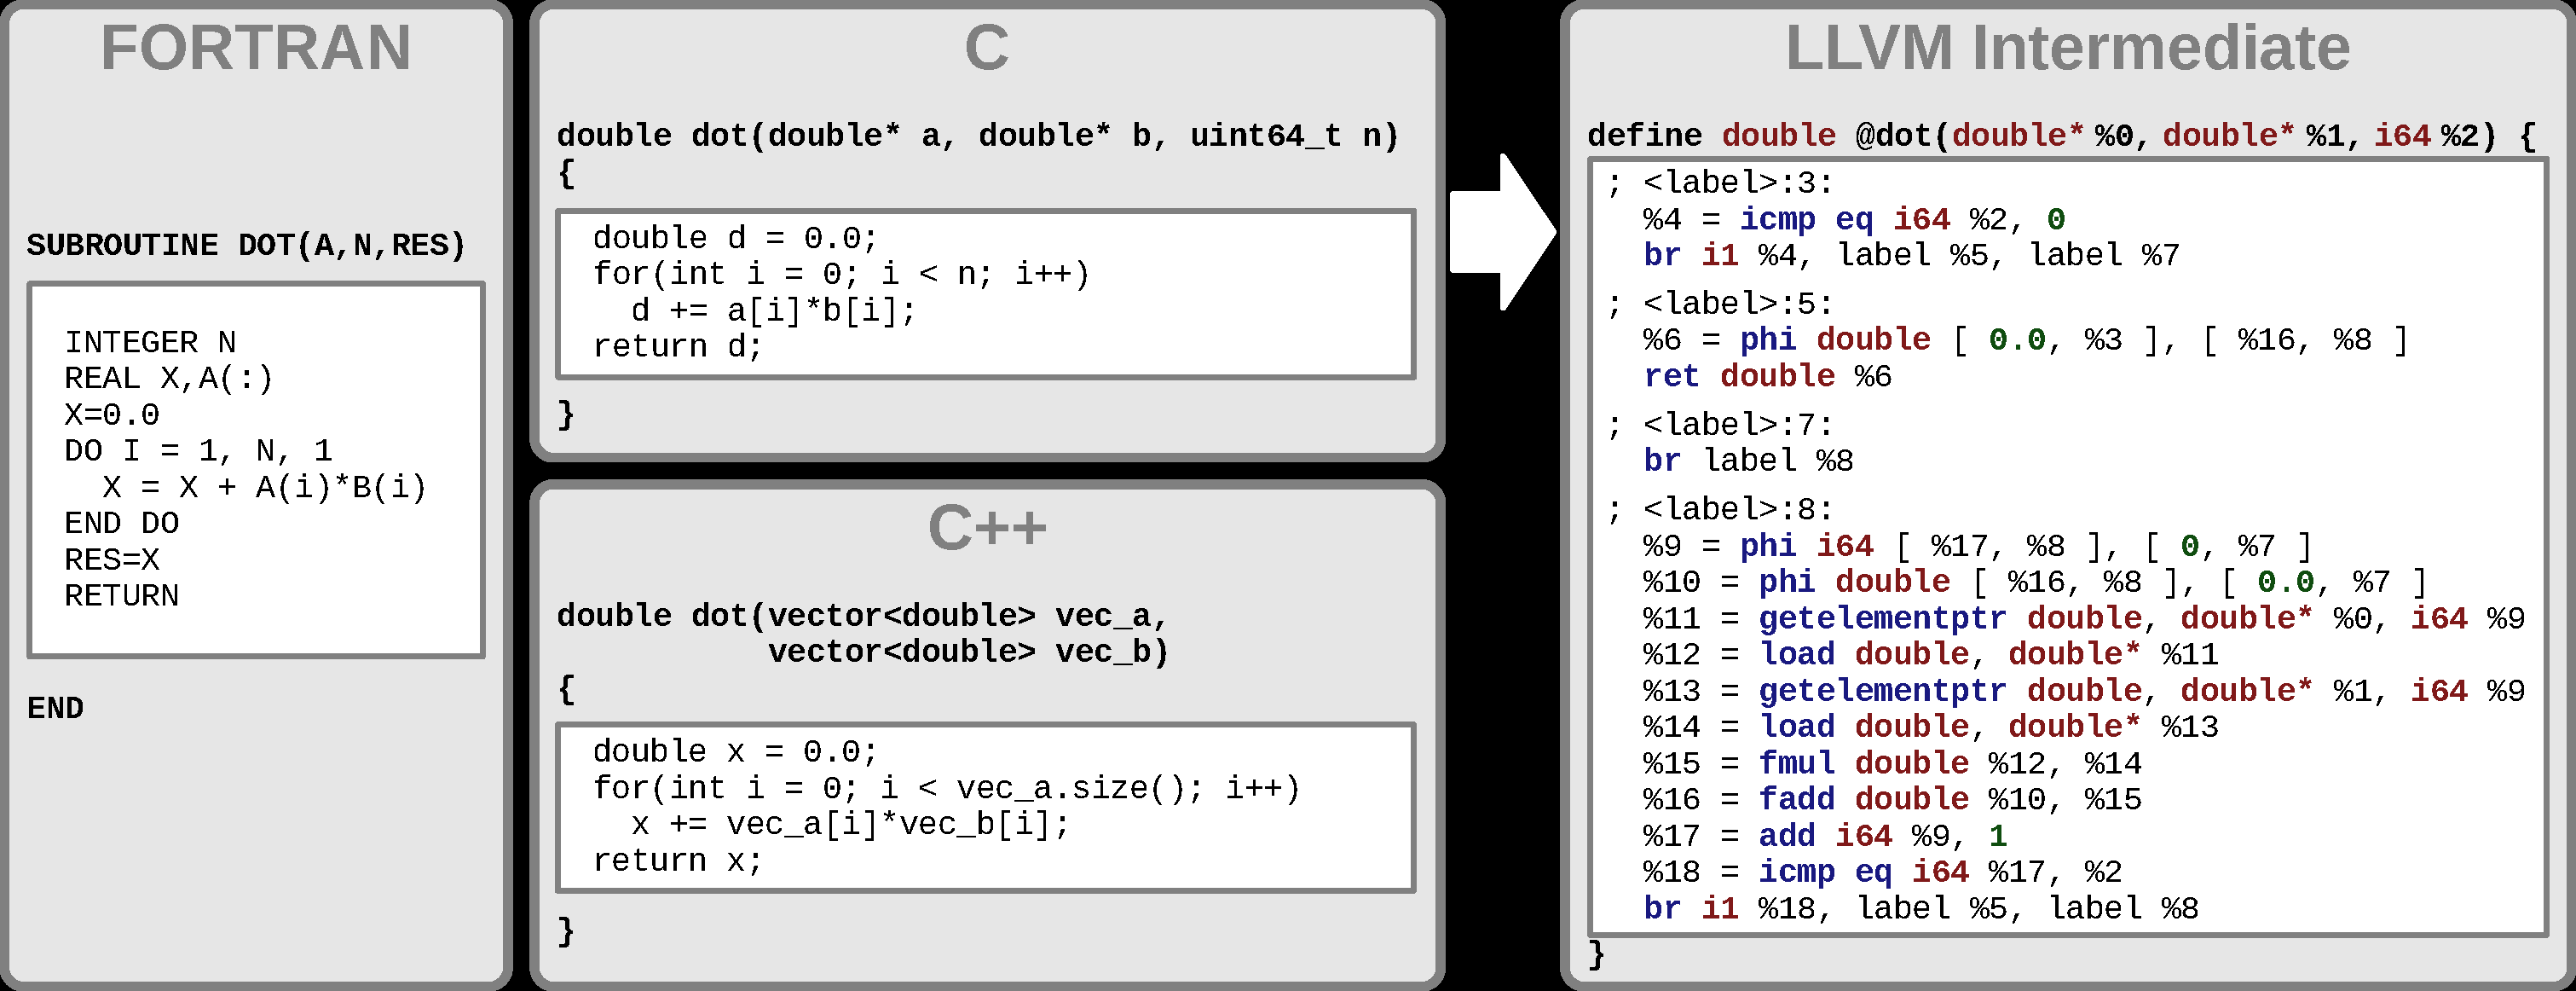
\includegraphics[width=\columnwidth]{figures/model_representations_textual}
\end{blackbox}

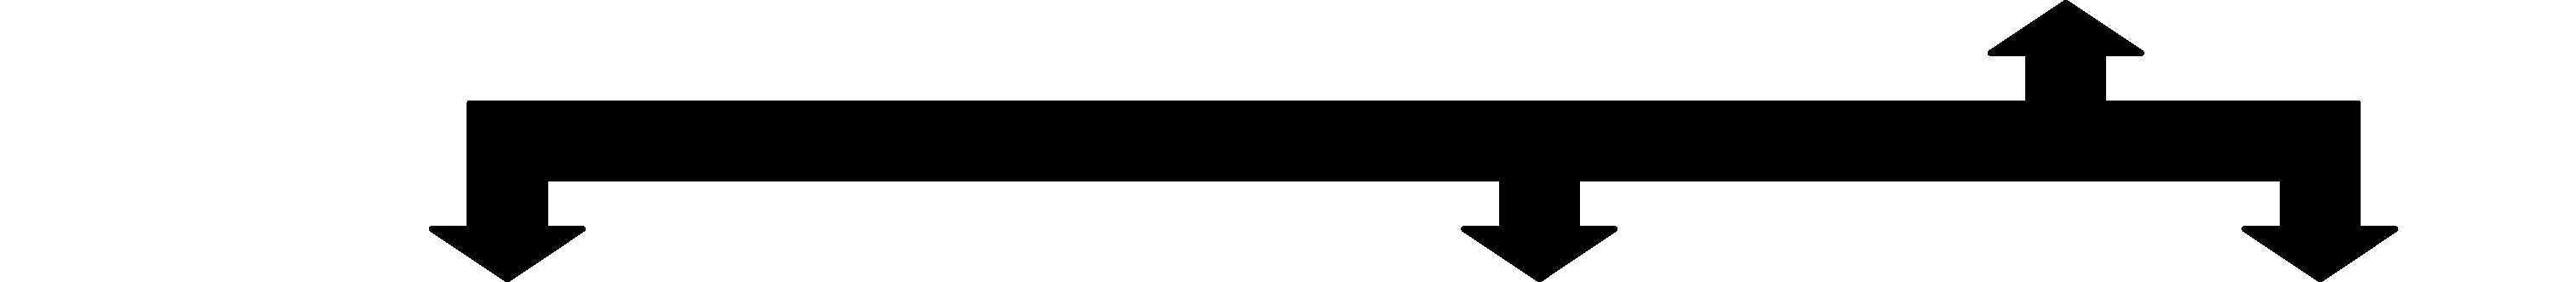
\includegraphics[width=\columnwidth]{figures/model_arrows_upper}

\begin{blackbox}{Data Structure Representation}
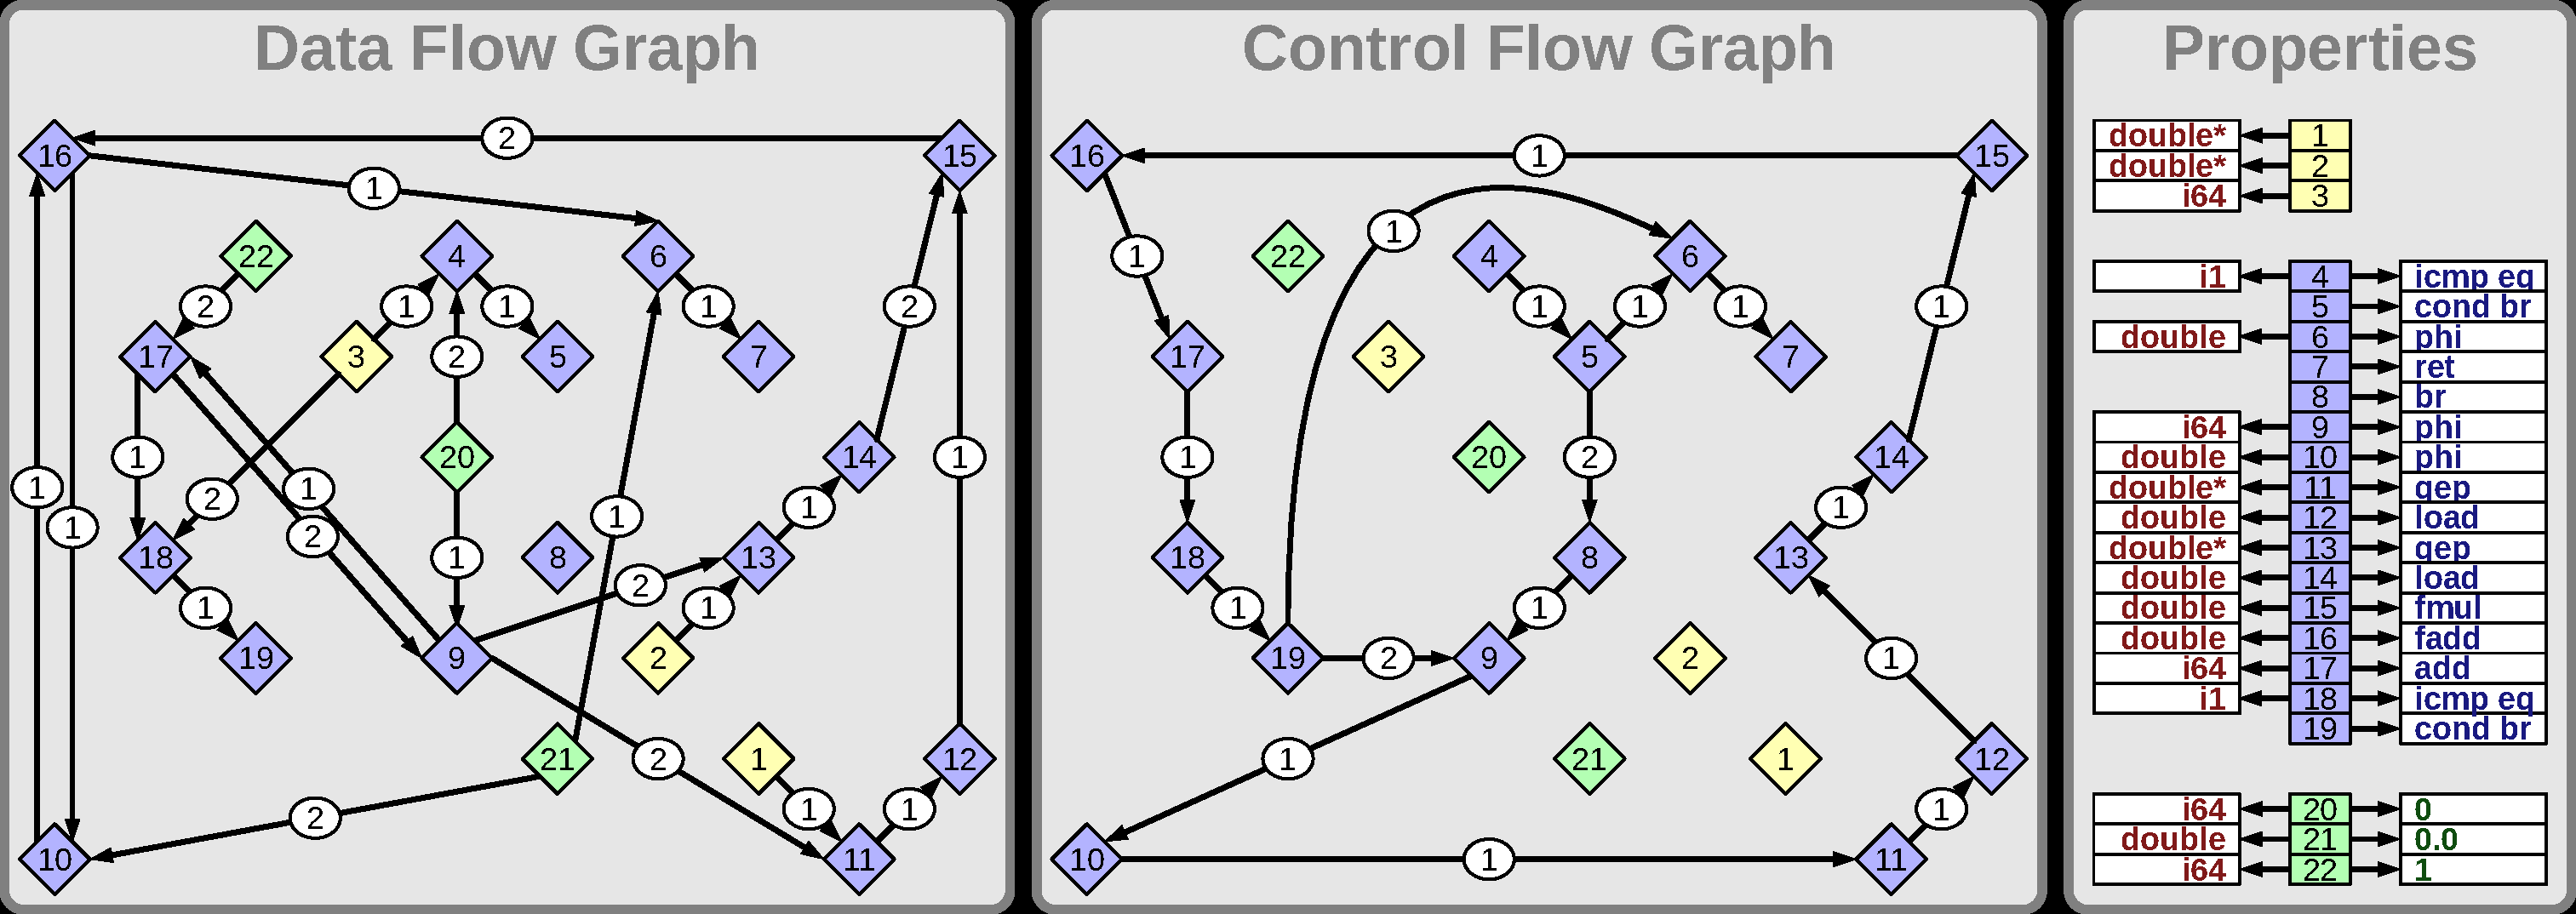
\includegraphics[width=\columnwidth]{figures/model_representations_structure}
\end{blackbox}

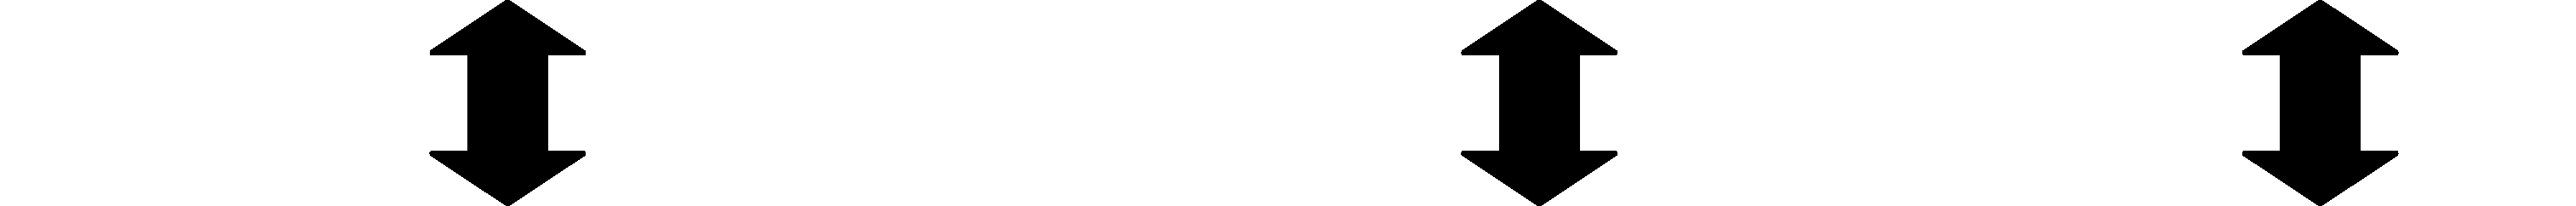
\includegraphics[width=\columnwidth]{figures/model_arrows_lower}

\begin{blackbox}{Mathematical Representation}
    \centering
    \begin{minipage}{0.329\textwidth}
        \begin{graybox}
            \scriptsize
            \setlength{\abovedisplayskip}{0pt}
            \setlength{\belowdisplayskip}{0pt}
            \vspace{-0.5em}
            \begin{align*}
                DF&G_\mathcal F=\{(1,11,1),(2,13,1)\\[-0.5em]
                  &(3,4,1),(3,18,2),(4,5,1),\\[-0.5em]
                  &(6,7,1),(9,11,2),(9,13,2),\\[-0.5em]
                  &(9,17,1),(10,16,1),(11,12,1),\\[-0.5em]
                  &(12,15,1),(13,14,1),(14,15,2),\\[-0.5em]
                  &(15,16,2),(16,6,1),(16,10,1),\\[-0.5em]
                  &(17,9,2),(17,18,1),(18,19,1),\\[-0.5em]
                  &(20,4,2),(20,9,1),(21,6,1),\\[-0.5em]
                  &(21,10,2),(22,17,2)\}\subset\mathbb N^3
            \end{align*}
        \end{graybox}
    \end{minipage}
    \begin{minipage}{0.329\textwidth}
        \begin{graybox}
            \scriptsize
            \setlength{\abovedisplayskip}{0pt}
            \setlength{\belowdisplayskip}{0pt}
            \vspace{-0.5em}
            \begin{align*}
                CFG_\mathcal F=\{&(4,5,1),(5,6,1),\\[-0.5em]
                  &(5,8,2),(6,7,1),\\[-0.5em]
                  &(8,9,1),(9,10,1),\\[-0.5em]
                  &(10,11,1),(11,12,1),\\[-0.5em]
                  &(12,13,1),(13,14,1),\\[-0.5em]
                  &(14,15,1),(15,16,1),\\[-0.5em]
                  &(16,17,1),(17,18,1),\\[-0.5em]
                  &(18,19,1),(19,6,1),\\[-0.5em]
                  &(19,9,2)\}\subset\mathbb N^3
            \end{align*}
        \end{graybox}
    \end{minipage}
    \begin{minipage}{0.329\textwidth}
        \centering
        \begin{graybox}
            \scriptsize
            \setlength{\abovedisplayskip}{0pt}
            \setlength{\belowdisplayskip}{0pt}
            \vspace{-0.5em}
            \begin{align*}
                T_\mathcal F={}&\{(1,\textit{double*}),(2,\textit{double*}),\dots\}\\[-0.5em]
                      \subset{}&\mathbb N\times Types_\text{LLVM}\\[-0.25em]
                P_\mathcal F={}&\{1,2,3\}\subset\mathbb N\\[-0.25em]
                I_\mathcal F={}&\{(4,\textit{icmp eq}),(5,\textit{cond br}),\dots\}\\[-0.5em]
                      \subset{}&\mathbb N\times Opcodes_\text{LLVM}\\[-0.25em]
                G_\mathcal F={}&\{\}\subset\mathbb N\\[-0.25em]
                C_\mathcal F={}&\{(20,0),(21,0),(22,1)\}\\[-0.5em]
                      \subset{}&\mathbb N\times\mathbb R
            \end{align*}

            \vspace{0.45em}
        \end{graybox}
    \end{minipage}

    \begin{minipage}{0.55\textwidth}
        \begin{graybox}
            \setlength{\abovedisplayskip}{0pt}
            \setlength{\belowdisplayskip}{0pt}
            \vspace{-0.5em}
            \begin{align*}
                M_{dot}=(DFG_\mathcal{F},
                 CFG_\mathcal{F},
                 T_\mathcal{F},
                 P_\mathcal{F},
                 I_\mathcal{F},
                 G_\mathcal{F},
                 C_\mathcal{F})
            \end{align*}
        \end{graybox}
    \end{minipage}
\end{blackbox}
\caption{Compiler-generated LLVM IR code is decomposed into data flow, control
         flow and per-value attributes.
         Mathematical notations of the three components are shown at the
         bottom.}
\label{fig:derivemaths}
\end{figure}

\section{Constraint Programming on SSA Programs}

    With a mathematical model of SSA programs in place, properties of such
    programs can now be formulated as constraint problems.
    For this purpose, \autoref{not:modelrepresentations} is introduced first,
    followed by the actual definition of {\em SSA constraint problem}s in
    \autoref{def:cprob}.

\begin{figure}[H]
\begin{notation}{Set of SSA Models}{modelrepresentations}
    Given a specific SSA representation (LLVM, Hydrogen, MIR, $\dots$), then
    denote $F$ the set of all valid functions that can be expressed in it.

    The {\em set of SSA models} $\mathcal M$ is defined as
    \begin{align*}
        \mathcal M := \{M\mid\exists\mathcal F\in F\colon M
                        \text{ is the SSA Model of }\mathcal F\}
    \end{align*}
\end{notation}

\begin{definition}{SSA constraint problem}{cprob}
    An SSA constraint problem $C=(V,P)$ is made up of a finite set of variables
    $V$ and a boolean predicate
    $P\colon\mathbb N^V\times\mathcal M\mapsto\{\text{true}, \text{false}\}$.
    The set of {\em constraint solutions} for a given constraint problem and a
    specific SSA model $M\in\mathcal M$ is given as
    \begin{align*}
        S(C,M) = \{s\in\mathbb N^V\mid P(s,M)=\text{true}\}.
    \end{align*}
\end{definition}
\end{figure}

    Some intuition is required here.
    The predicate function $P$ takes two arguments, firstly a tuple of integers
    and secondly a model of a function.
    The finite set $V$ identifies the elements withing the tuples, it can be
    thought of as a set of labels.
    The tuples of integers in $\mathbb N^V$ correspond to tuples of values
    within the function.
    The predicate function determines whether these values stand in a specific
    relationship to each other.
    Finally, the set of constraint solutions lists all those tuples, for which
    the predicate holds.

    The two parameters of $P$ -- integer tuple and model -- should be
    interpreted as two very different beasts here.
    The predicate evaluates whether a condition holds for the tuple of integers,
    the model on the other hand serves as the context for this evaluation.
    This is reflected in the definition of the set of constraint solutions,
    which is the set of all {\em true} evaluations given a fixed model.
    More pointedly, it makes sense to query ``all loops in a given function'',
    yet to ask for ``all functions with a specific loop'' is meaningless.

    The interesting aspect of this defition is now the structure of predicates
    $P$.
    This section will concern it self with how meaningful predicates can be
    composed from small building blocks and how the internal structure of the
    predicate can lead to efficient solver approaches.
    In order to evoke an intuition about these challenges, there will first be
    an example.

\subsection{Constraint Program Example}

\begin{figure}[p]
    
\raggedright
{\bf(a)} {} Initial problem statement:\\[1em]

\centering
{\LARGE$\underbrace{\text{Detect\vphantom{p}}}
                  _{\text{solver }S}
      \ \underbrace{\text{simple loop iterators}}
                  _{\text{SSA constraint problem }(V,C)}
                  \ \text{in the}
      \ \underbrace{\text{dot product function}}
                  _{\text{SSA model }M_{dot}}
                    \text{.}$}\\[2em]

\raggedright
{\bf(b)} {} Formulation as constraint problem:\\[1em]

\centering
\fontsize{60}{0}$S{}$\fontsize{20}{0}$\left(
\begin{minipage}{0.8\textwidth}
    \normalsize
    \begin{blackwhitebox}{\Large SSA constraint problem}
        \setlength{\abovedisplayskip}{0pt}
        \setlength{\belowdisplayskip}{0pt}
        \vspace{-0.5em}
        \begin{align*}
            V={}&\{\text{phi}, \text{update}, \text{step}\}\\
            C(M,x)={}&    ((1,x_\text{step})
                            \in C_\mathcal{F}\mathrel\land
                           (add,x_\text{update})
                            \in I_\mathcal{F}\mathrel\land\\
               &\phantom{(}(x_\text{phi},x_\text{update})
                            \in DFG_\mathcal{F}^*\mathrel\land
                           (x_\text{step},x_\text{update})
                            \in DFG_\mathcal{F}^*\mathrel\land\\
               &\phantom{(}(x_\text{update},x_\text{phi})
                            \in DFG_\mathcal{F}^*\mathrel\land
                           (phi,x_\text{phi})
                            \in I_\mathcal{F})
        \end{align*}
    \end{blackwhitebox}
    \begin{blackwhitebox}{\Large SSA model}
        \setlength{\abovedisplayskip}{0pt}
        \setlength{\belowdisplayskip}{0pt}
        \vspace{-0.5em}
        \begin{align*}
            DF&G_\mathcal F=\{(1,1,11),(1,2,13),(1,3,4),(2,3,18),(1,4,5),(1,6,7),\\[-0.5em]
              &(2,9,11),(2,9,13),\underline{(1,9,17)},(1,10,16),(1,11,12),(1,12,15),\\[-0.5em]
              &(1,13,14),(2,14,15),(2,15,16),(2,16,6),(2,16,10),\underline{(2,17,9)},\\[-0.5em]
              &(1,17,18),(1,18,19),(2,20,4),(1,20,9),(1,21,6),(1,21,10),\\[-0.5em]
              &\underline{(2,22,17)}\}\\[-0.25em]
            CF&G_\mathcal F=\{(1,4,5),(1,5,6),(2,5,8),(1,6,7),(1,8,9),(1,9,10),\\[-0.5em]
              &(1,10,11),(1,11,12),(1,12,13),(1,13,14),(1,14,15),\\[-0.5em]
              &(1,15,16),(1,16,17),(1,17,18),(1,18,19),(1,19,6),(2,19,9)\}\\[-0.25em]
            T_\mathcal F&{}=\{(\textit{double*},1),(\textit{double*},2),\dots\}\\[-0.25em]
            P_\mathcal F&{}=\{1,2,3\}\\[-0.25em]
            I_\mathcal F&{}=\{(\textit{icmp eq},4),(\textit{cond br},5),(\textit{phi},6),(\textit{ret},7),(\textit{br},8),\underline{(\textit{phi},9)},\\[-0.5em]
                        &(\textit{phi},10),(\textit{gep},11),(\textit{load},12),(\textit{gep},13),(\textit{load},14),(\textit{fmul},15),\\[-0.5em]
                        &(\textit{fadd},16),\underline{(\textit{add},17)},(\textit{icmp eq},18),(\textit{cond br},19)\}\\[-0.25em]
            G_\mathcal F&{}=\{\}\\[-0.25em]
            C_\mathcal F&{}=\{(0,20),(0,21),\underline{(1,22)}\}
        \end{align*}
    \end{blackwhitebox}
\end{minipage}
\right)$\\[2em]

\raggedright
\normalsize
{\bf(c)} {} Resulting set of constraint solutions:\\[1em]

\centering
{\LARGE$S_{M_{dot}}(V,C)=\{\{\text{phi}\mapsto9,
                             \text{update}\mapsto17,
                             \text{step}\mapsto22\}\}\subset\mathbb N^V$}
\caption{Detection of simple loop iterators is formulated as a constraint
         problem and applied to the SSA model from \autoref{fig:derivemaths}.
         One solution corresponding to the source variable {\tt i} is found.}
\label{fig:constraintsolution}
\end{figure}

    Consider the task of detecting in a program all simple loop iterator in a
    function, shown in \autoref{fig:constraintsolution}.
    The top {\bf a)} demonstrates how this can be translated into a constraint
    problem, solved in the context of an SSA model.
    For demonstration purposes, the SSA model that was derived in
    \autoref{fig:derivemaths} is used.

    Simple loop iterators show up in LLVM IR as data flow cycles with a phi node
    and an add instruction.
    This is expressed as a constraint problem at the top of the second part
    {\bf b)} of the figure.
    The formulation introduces the variables
    $V=\{\text{phi}, \text{update}, \text{step}\}$ and a predicate to
    describe the required conditions on the variables.
    The predicate is decomposed with logical conjunctions (``$\land$'') into
    several {\em elemt-of} relationships that have to hold simultaneously on the
    structures of the model.
    Explicit control flow constraints for establishing the loop strucure are not
    required, as the data flow with the $\Phi$ node already implies the presence
    of a loop structure.
    Below the predicate formulation is the SSA model from
    \autoref{fig:derivemaths}.

    At the bottom {\bf c)} of the figure, the set of constraint solutions is
    shown.
    It contains as its only element the tuple
    $\{\text{phi}:6,\text{update}:14,\text{step}:19\}$.
    Note that elements of $\mathbb N^V$ can be identified as mappings
    $V\rightarrow\mathbb N$.
    The underlined strucures in the lower part of
    \autoref{fig:constraintsolution} {\bf b)} demonstrate the validity of the
    solution:
    $(22,1)\in C_\mathcal F$ and $(9,17,1)\in DFG_\mathcal F$ and
    $(22,17,2)\in DFG_\mathcal F$ and $(9,\textit{phi})\in I_\mathcal F$ and
    $(17,\textit{add})\in I_\mathcal F$ and $(17,9,2)\in DFG_\mathcal F$,
    corresponding to the six simple constraints that make up the predicate.

    Each solution therefore assigns an integer to each variable.
    With the help of \autoref{fig:derivemaths}, the specific values $9,17,22$
    can be identified with lines 14 and 17, as well as the constant 1 in the
    LLVM IR code from \autoref{llvmirexample} {\bf b)}.
    This corresponds to the loop iterator \texttt{i} in the C source code of the
    \texttt{dot} function, correctly identifying the only simple loop iterator.

    With a detailed derivation of the SSA model completed and some intuition
    about the nature of constraint problems, only the solver $S$ in
    \autoref{fig:constraintsolution} remains a black box.
    The next sections derive how a backtracking solver can
    be used to efficiently compute the set of solutions.

\subsection{Solving of SSA Constraint Problems}

    The aim of a solver for SSA constraint problems is to compute the set of
    solutions $S(C,M)$ for some concrete values of $C$ and $M$.
    This is fundamentally a search problem: the space of $\mathbb N^V$ has to be
    searched for values satisfying $P$.
    The size of $\mathbb N^V$, wich is countable but infinite, requires
    non-trivial computational approaches to this problem, even when the direct
    evaluation of $P$ can be efficiently performed.

    On top of that, an algorithmic solution requires an intelligent way to
    encode the boolean predicate.
    It is intuitive and well established in literature to use backtracking for
    solving constraint problems, so firstly this will be reformulated
    recursively as follows.
    The finite set of $V$ can be enumerated $V=\{v_0,v_1,\dots,v_n\}$.

    Then consider $C_k=(V_k,P_k)$, where $P_k$ is defined as
    \begin{align*}
        P_k(x)=\left\{\begin{array}{l}\text{true} if P(x,y)=true for some y\\
                                      \text{false} otherwise\end{array}\right.
    \end{align*}

    Consider the following purely algebraic reformulation.
    \begin{align*}
        S_k=\{\emptyset\}\\
        S_{k+1}(C,\mathcal F)=&\{s\in\mathbb N^V_k\mid P(s,\mathcal F)=\text{true}\}\\
                             =&\{
    \end{align*}

\subsection{Structure of SSA Constraint Problems}

    Predicates for useful SSA constraint problems are composed by logical
    connectors from a limited set of {\em atomic} predicates, that cannot
    further be decomposed.
    The atomic predicates are defined directly on the mathematical model and
    they often only utilize a very small set of variables, typically one or two.
    Many of then are simple element-of relationships for the different
    components in the SSA model.
    In the previous example, this was true for all the atomic constraints.

    There are some important compiler analysis problems that can not not be
    decomposed with logical connectors into atomic predicates using only one
    or two variables.
    They are mostly concerned with graph properties and we will discuss some of
    them in detail later in this chapter.
    For the purposes of constraint solving, these are more difficult to handle.

    Via the logical connectors $\land$ and $\lor$, the atomic predicates
    interact on their shared variables.
    There will be some additional high level connectors introduced later, which
    appriximate logical operators from first order logic.

\section{Implementation of Constraint Predicates}

    With the solver approach derived, it now needs to be established how real
    constarint problem predicates can be algorithmically implemented in order
    to evaluate the required functions.

\subsection{Important Graph Properties}

    With our established notation, we can now transfer standard compiler
    analysis problems into this more formal language.
    Most of these are based on graph theoretic considerations, so we
    will firstly need to recapitulate some graph theory basics.
    Firstly, there is the notion of {\em cuts} of graphs, that we will introduce
    here in a hybrid version of edge based and vertex based modelling.

    \begin{definition}{Connections and Cuts}{def:cuts}
        Consider an adjacency set $E\subset\mathbb{N}\times\mathbb{N}$ of a
        directed graph and let $a,b\in\mathbb{N}$.
        \newline
        A {\em connection} between $a$ and $b$ in $E$ is a subset
        $A\subset\mathbb{N}$ such that a finite sequence $c_1,\dots,c_n$
        exists with
        \begin{gather*}
            a=c_1\hspace{1cm}c_2,\dots,c_{n-1}\in A\hspace{1cm}b=c_n\\
            (c_k,c_{k+1})\in E\hspace{1em}\text{for all}\hspace{1em}k=1,\dots,n-1.
        \end{gather*}
        A {\em cut} between $a$ and $b$ in $E$ is a subset $B\subset E$
        such that no {\em connection} between $a$ and $b$ in $E\setminus B$
        exists.
        We define the {\em set of cuts} between $a$ and $b$ in $E$ as
        \begin{align*}
            \text{Cuts}_E(a,b):=\{B\subset E\mid B\text{ is {\em cut} between $a$ and $b$ in $E$}\}
        \end{align*}
    \end{definition}

    These notions are quite intuitive, two vertices in a graph have a connection
    if one can reach the other via the available edges and by ``cutting'' these
    edges, they are no longer connected.

    These definitions are very useful in order to identify crucial properties of
    data and control flow graphs.
    Most standard is the the definition of a dominator in the control flow
    graph: An instruction $d$ is said to dominate another instruction $n$ if
    every path from the entry node to $n$ through the control flow graph must
    go through $d$.
    In our model this is of course equivalent to the following:

    \begin{definition}{Dominator}{def:dominator}
        Consider an instruction $n$ in a function $\mathcal F$.
        A {\em dominator} of $n$ in $\mathcal{F}$ is an instruction $d$ such
        that $\{(d,m)\mid(d,m)\in CFG_\mathcal{F}^*\}$ is a {\em cut} between $1$ and $n$ in $CFG_\mathcal{F}^*$.
    \end{definition}

    Another important definition is the concept of control dependence.
    Control dependence models the behaviour of conditional control flow.
    Instructions that are executed only in some control flow paths are control
    dependent on the conditional branches that preceed them.

    \begin{definition}{Control Dependence}{cdg}
        Consider instructions $a,b$.
        We say that an $b$ is control dependent on $a$ if a instructions
        $c,c'$ exist such that $(a,c),(a,c')\in CFG_\mathcal{F}^*$ and
        \begin{align*}
            \{(a,c)\}\in{}&{}\text{Cuts}_E(a,b)\\
            \{(a,c')\}\notin{}&{}\text{Cuts}_E(a,b)\text{.}
        \end{align*}
        We define the {\em control dependence graph} as follows
        \begin{align*}
            CDG_\mathcal{F}:=\{(a,b)\in\mathbb{N}^2\mid b\text{ control dependent on }a\}
        \end{align*}
    \end{definition}

\begin{figure}[p]
    \centering
    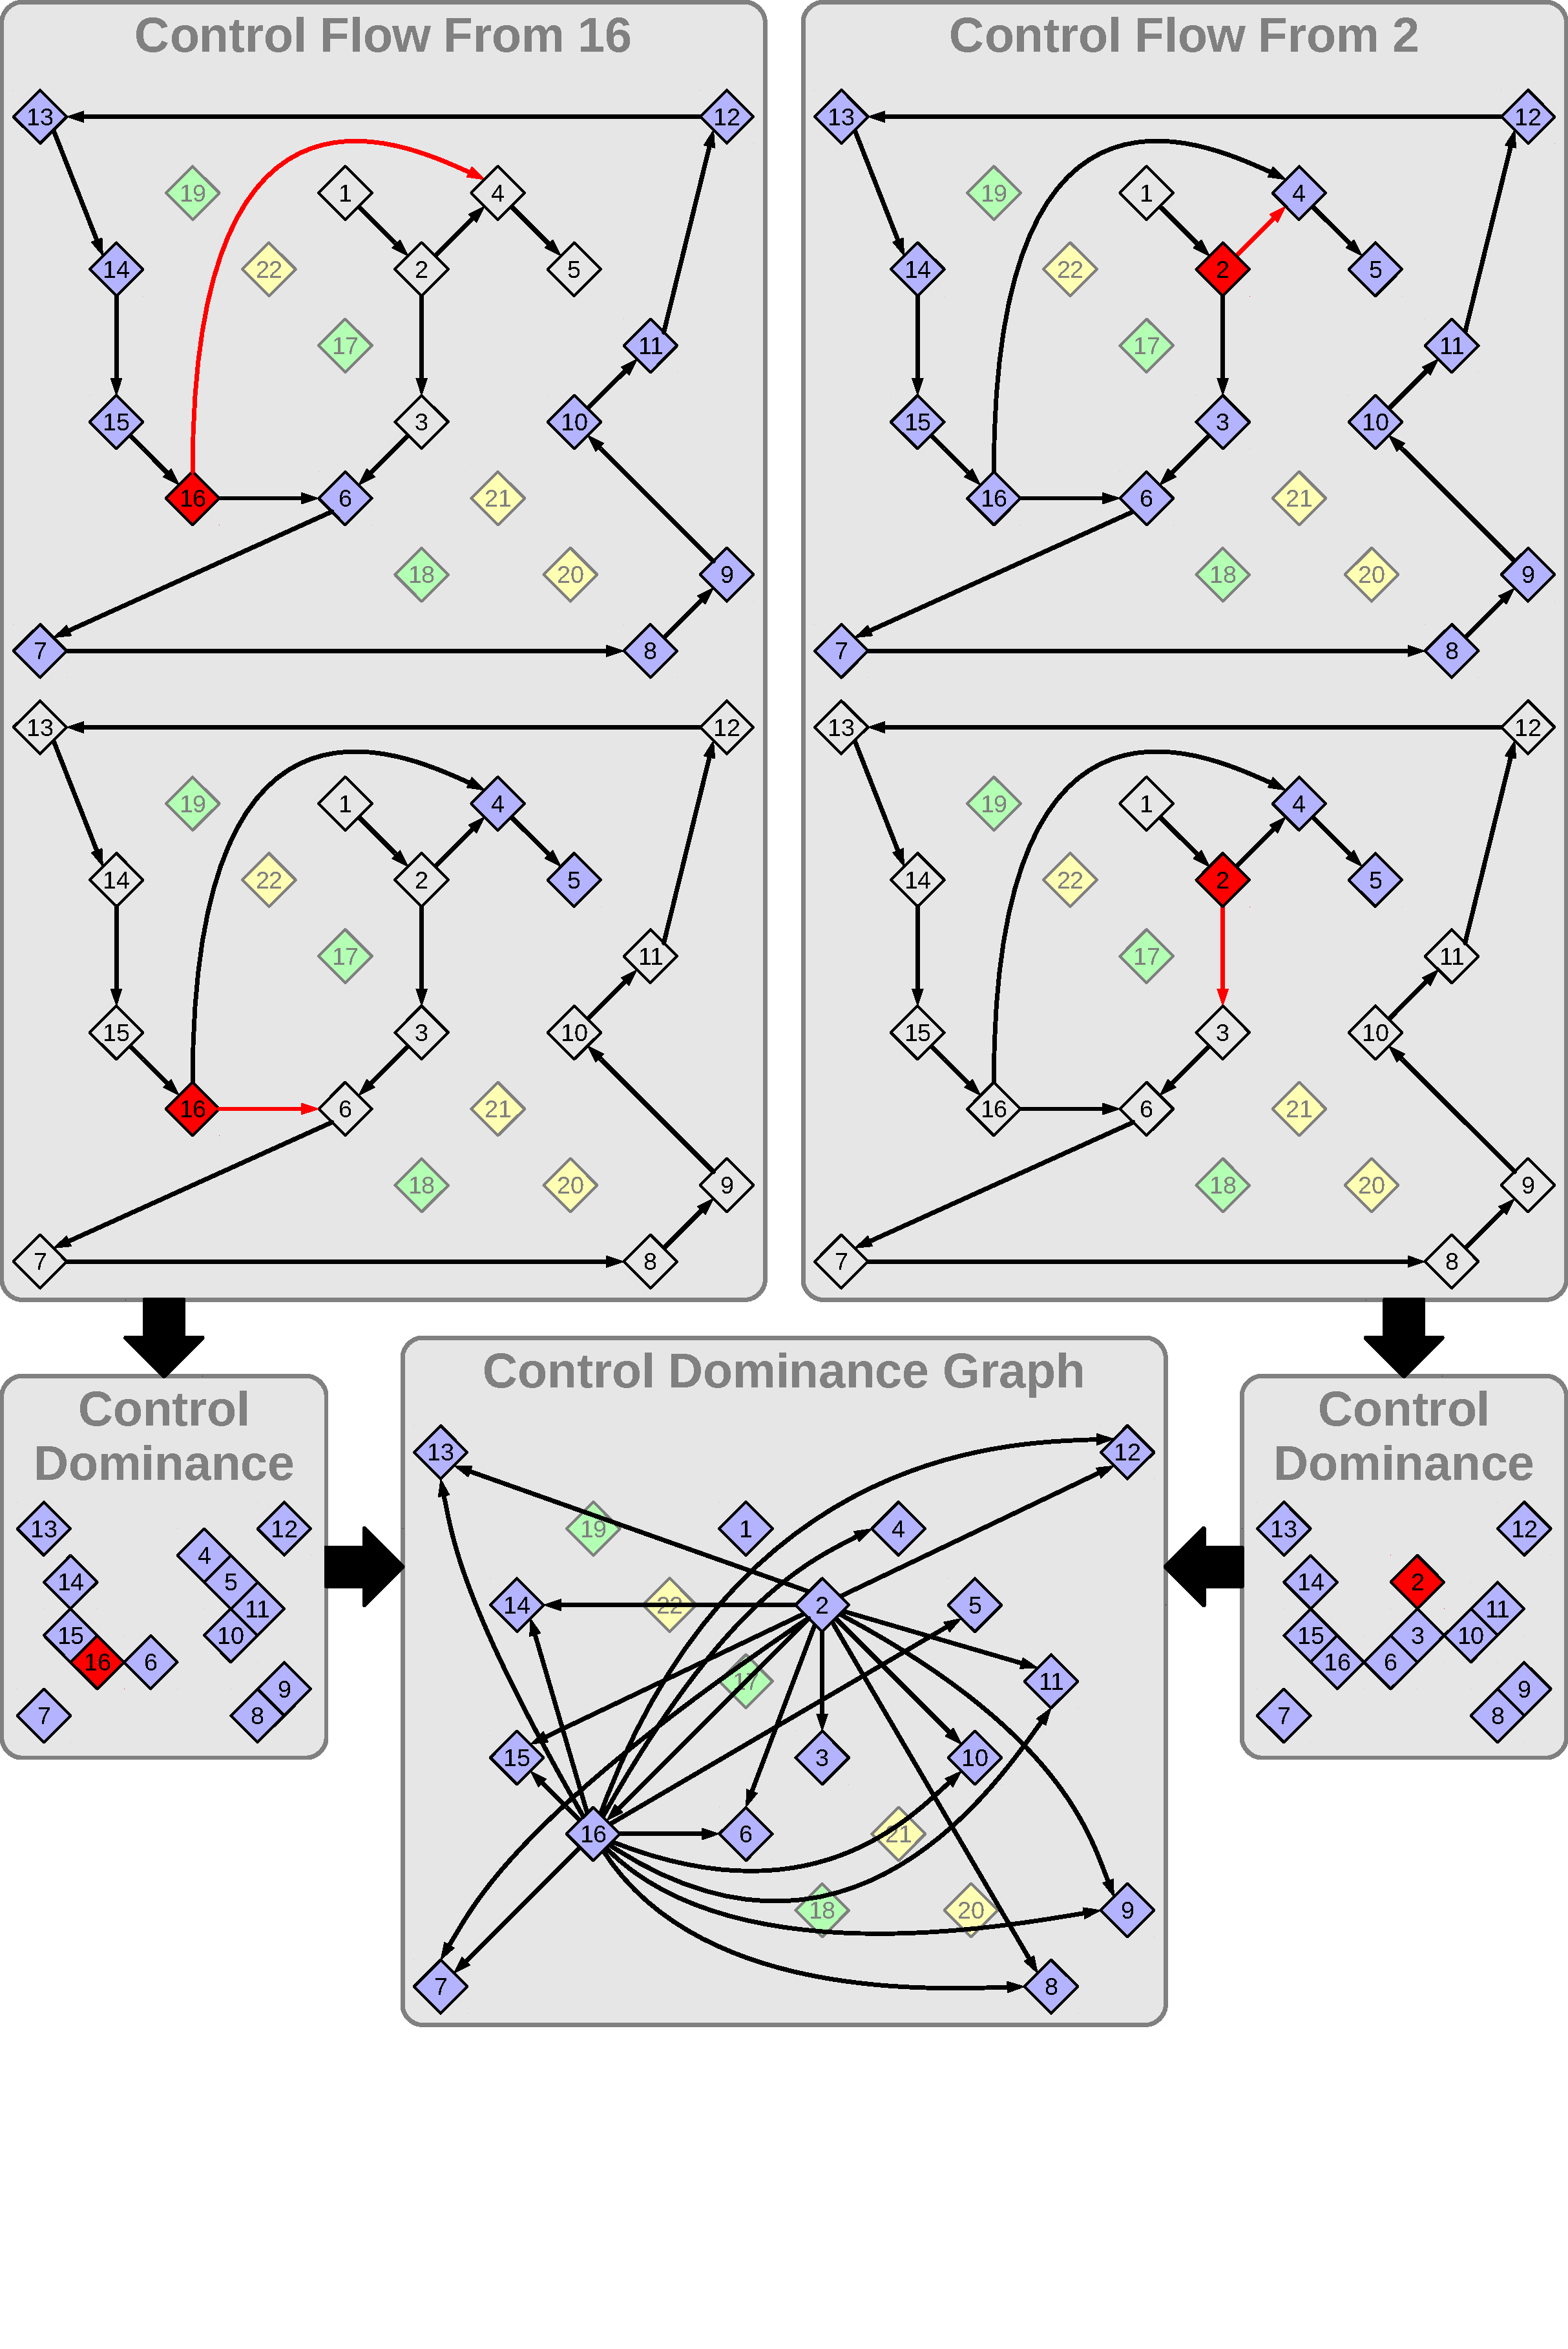
\includegraphics[width=\textwidth,height=1.5\textwidth]{figures/schaubild2.pdf}

    \vspace{27.38136pt}
    \caption{Computation of the control dependence graph.}
    \label{fig:pdg}
\end{figure}

\subsection{Control Dependence Example}

    The control dependence graph is a function of the control flow graph, as is
    directly apparent from \autoref{def:cdg}.
    We can see how an example control dependence graph is computed in
    \autoref{fig:pdg}, from the control flow graph of the \texttt{dot} function
    in \autoref{fig:derivemaths}.
    From the definition it is immediately obvious that we need to only consider
    conditional branches as origins of control dependence.

    We can consider the two conditional branches $2$ and $16$ independently.
    On the right, we consider only $2$.
    We check the defining property: On the top of the figure, all the
    instructions that are not reachable from $2$ without the edge $(2,4)$ are in
    grey.
    Below this, all instructions not reachable from $2$ without $(2,3)$ are
    grey.
    We see that $4,5$ are always reachable and $1$ is never reachable, these are
    therefore not control dependent on $2$.
    All the other instructions are control dependent on $2$.

    Once we have computed this for all conditional branches, we take the union
    on graphs and get the complete control dependence graph of the function.
    Note what this graph represents:
    Once the loop in the function has been unrolled, it contains a conditional
    and a loop.
    Eveything within the body of the conditional is control dependent on $2$.
    Everythig within the loop as well as everything afterwards is control
    dependent on $16$.

\subsection{Phi Dependence Graph}

    Phi nodes are fundamental in single static assignment form and need special
    care.
    The value that a phi node takes depends on from where a phi node was
    reached.
    We need to encapsulate this in a graph.

    \begin{definition}{Phi Dependence Graph}{def:pog}
        Let $p$ a phi node and $c$ a conditional branch instruction.
        We say that the outcome of $p$ depends on $c$ if there is a branch
        instruction $b$ that reaches $p$ such that $b$ is control dependent on
        $c$.

        This defines the {\em phi dependence graph} $\Phi DG_\mathcal{F}$.
    \end{definition}

\subsection{Program Dependence Graph}

    After the control flow, data flow and control dependence graph, we lastly
    introduce the {\em program dependence graph}.
    It is the most exhaustive tool that we have to describe how values depend on
    each other.

    \begin{definition}{Program Dependence Graph}{def:pdg}
        The {\em program dependence graph} is defined as the union of data flow
        and control dependence graphs.
        \begin{align*}
            PDG_\mathcal{F}:=DFG_\mathcal{F}^*\cup CDG_\mathcal{F}^*\cup\Phi DG_\mathcal{F}\text{.}
        \end{align*}
    \end{definition}

    With the program dependence graph, we can now define subsections of the
    program that are self-contained and can be separated into their own
    function.
    This works even if they contain complicated control flow.
    Firstly, we need a definition of an interface.

    \begin{definition}{Interface}{def:interface}
        Let $a\in CFG_\mathcal{F}^*$ and $b_1,\dots,b_n\in DFG_\mathcal{F}^*$.
        Furthermore let $A\subset\mathbb{N}$ a set of instructions.

        We say that $(b_1,\dots,b_n)$ is an interface to $A$ if it is a cut
        between $o$ and $A$ in $PDG_\mathcal{F}$ for any of the following $o$:
        \begin{itemize}
            \item $o$ is a paramter
            \item $o$ is impure
        \end{itemize}
    \end{definition}

\newpage
\subsection{Interface Example}

    We will now consider a non-trivial example.
    Consider this snppet of C code, implementing a function that performs a
    simple square root approximation on each element in an array of double
    precision floating point values.

\begin{figure}[ht]
\begin{lstlisting}[language=C]
void map_sqrt(size_t length, double* array)
{
    for(int i = 0; i < length; i++)
    {
        double root = 1.0;
        for(int i = 0; i < 10; i++)
            root = 0.5*(root+array[i]/root);

        array[i] = root;
    }
}
\end{lstlisting}
\caption{{\bf map$\circ$sqrt}: Apply an appriximate sqare root function to each
         element in a vector.}
\end{figure}

    Coneptually, we should be able to disentangle the square root function from
    the control flow of the outer loop.
    This is possible with the preceeding definition of {\em interfaces}.

\newpage
In single static assignment form, this code looks as follows:

\begin{lstlisting}[language=LLVM]
define void @map_sqrt(i64, double*) {
  %3 = icmp eq i64 %0, 0
  br i1 %3, label %5, label %4

; <label>:4:
  br label %6

; <label>:5:
  ret void

; <label>:6:
  %7 = phi i64 [ %10, %8 ], [ 0, %4 ]
  br label %12

; <label>:8:
  %9 = getelementptr double, double* %1, i64 %7
  store double %19, double* %9
  %10 = add nuw i64 %7, 1
  %11 = icmp eq i64 %10, %0
  br i1 %11, label %5, label %6

; <label>:12:
  %13 = phi i64 [ 0, %6 ], [ %20, %12 ]
  %14 = phi double [ 1.0, %6 ], [ %19, %12 ]
  %15 = getelementptr inbounds double, double* %1, i64 %13
  %16 = load double, double* %15
  %17 = fdiv double %16, %14
  %18 = fadd double %14, %17
  %19 = fmul double %18, 5.0
  %20 = add nuw nsw i64 %13, 1
  %21 = icmp eq i64 %20, 10
  br i1 %21, label %8, label %12
}
\end{lstlisting}

    In this example, the set $\{\%9\}$ is an interface to $\{(\%19,\%store)\}$.

\section{Formulating Constraint Problems}

    With this mathematical background, it is now possible to derive constraint
    programming on top of LLVM code.

    Consider the following definitions of simple binary predicates:

    \begin{align*}
     is\_branch\_inst(\mathcal F, n):= (n,\text{\bf br})\in T_\mathcal{F}\\
     is\_control\_edge(\mathcal F, n, m):= (n,m)\in CFG_\mathcal{F}^*\\
     is\_control\_dom(\mathcal F, n, m):= \\
    \end{align*}

    We can then use these predicates to define more complex constructs, such as
    single entry, single exit (SESE) regions.

    \begin{definition}{}{}{}
        A single entry single exit region is a tuple $a,b,c,d\in\mathcal N$ such
        that the following properties hold:
        \begin{align*}
            is\_control\_edge(\mathcal{F},a,b)\\
            is\_control\_edge(\mathcal{F},c,d)\\
            is\_control\_dom(\mathcal{F},c,d)\\
            is\_control\_postdom(\mathcal{F},d,c)\\
        \end{align*}
    \end{definition}


\chapter{Contraint Programming on Static Single Assignment Code}
    \label{chapter:theory}
    
    Four areas of research are of particular relevance to this thesis:
    {\bf Constraint programming and specification languages} are central to the
    introduced methodology.
    The relevant literature includes the research into constraint programming in
    the context of program analysis and the design of specification languages.
    The survey of previous approaches to
    {\bf compiler analysis and auto-parallelisation}
    establishes the baselines for the later evaluation sections.
    Related work on {\bf heterogeneous computing} motivates the proposed
    approaches, by presenting the plethora of other programming paradigms to
    overcome the specific challenges of emerging hardware.
    Lastly, the diverse research landscape around concepts related to
    {\bf computational idioms} puts the algorithmic structures that are detected
    in later chapters of this thesis into context.

\section{Constraint Programming and Specification Languages}

    Declarative Languages, constraint programming, and the application of
    constraints to program analysis problems are well-established in the
    literature.
    Previous work covers query languages, logic programming, applications to
    software security and formal verification, model checking and SMT,
    but also more compiler-centric data flow analysis and type inference
    problems.
    The limited scope of this section requires a focus on work that is
    particularly relevant to this thesis.

    For this research, constraint programming is most interesting within the
    context of research fields such as program analysis and model checking.
    Crucial background material for this thesis also comes from
    the programming language design community of declarative programming
    languages.
    Prolog and its many extensions and dialects particularly stand out as
    fully-fledged logic programming languages, but parallels can also be drawn
    to querying languages that apply database techniques to static analysis.

    These different fields vary significantly in their interests, motivations,
    and approaches, but the underlying challenges are often similar.
    Notably, the performance of backtracking solvers and the scalability to
    complex problems are a recurring theme.

\subsection{Constraint Programming for Program Analysis}

    \paragraph*{Constraint analysis on abstract languages}
    Constraint systems have long been used for program analysis.
    \citet{Aiken:1999:ISC:339853.339897} gives a comprehensive overview of
    earlier work, highlighting the crucial ability of constraint-based program
    analysis to separate {\it constraint specification} from
    {\it constraint resolution}.
    This separation is critical also for this thesis, as it enables the
    scalability of compiler analysis problems beyond what could reasonably be
    implemented with manual recognition routines.
    The constraint specification can be formulated briefly, by offloading the
    {\it constraint resolution} to a separate solver.
    However, the article does not present any techniques to capture higher-level
    algorithmic concepts like computational idioms.
    Instead, it focuses on more basic compiler analysis problems, such as
    data flow analysis and type inference.

    More recent work on constraint-based program analysis by
    \citet{Gulwani:2008:PAC:1375581.1375616} leverages the advancements in
    modern off-the-shelf SAT/SMT solver technology.
    The analysis problems are lowered to bit-vector formulations, and the
    {\it constraint resolution} is entirely externalised to independently
    developed SMT solvers.
    The motivation of the approach is mainly to verify program properties,
    as opposed to the application of parallelising code transformation in this
    thesis.
    Furthermore, \Cref{sec:SATcomp} showed that the confinement to
    conventional SMT solvers is inefficient for the resolution of
    SSA constraint problems.

    \citet{Kundu:2009:POC:1543135.1542513} propose constraints to verify the
    correctness of program transformations with their system for
    Parameterized Equivalence Checking (PEC).
    This system improves on previous work performing translation validation.
    Translation validation is the validity checking of transformations on
    concrete input programs by comparing the semantics before and after
    modification.
    PEC implements a hybrid approach that allows some aspects of the program
    to be underspecified, yet does not check the soundness of transformations
    in full generality.
    The checking is done via a custom solver for the generated constraint
    problems.
    The hybrid nature allows the system also to validate program transformations
    that significantly modify the control flow, e.g.\ loop unswitching.
    However, it cannot discover transformation opportunities, only verify them
    after the transformation was applied.

    \paragraph*{Constraint analysis on compiler IR code}
    There is previous work on using constraint-based program analysis for real
    compiler intermediate representations, mostly in the area of security and
    the formal verification of software systems.
    This includes investigations into using SMT on LLVM intermediate
    representation, which is also used for the implementations in this thesis.
    \citet{Zhao:2012:FLI:2103656.2103709} built a model of LLVM IR for such
    solvers.
    However, this model serves an entirely different purpose to the SSA model
    of this thesis.
    The model provides operational semantics, but cannot be used to detect
    large-scale algorithmic structures in user programs, as is required for
    automatic heterogeneous acceleration.
    Instead, the focus is on formally verifying the correctness of existing
    compiler transformations for all possible user input.

    Recent domain-specific languages, such as Alive
    \citep{Lopes:2015:PCP:2737924.2737965}, operate on subsets of LLVM IR.
    The individual instructions are reformulated on bit-vectors, and the
    correctness of conditions is checked with an SMT solver.
    However, Alive only implements a subset of LLVM's integer and pointer
    arithmetic instructions.
    It has no support for control flow and does not scale to the applications
    that are used in this thesis for evaluation.
    Instead, it is designed for formally verifying already existing
    compiler optimisations that operate on only a handful of integer
    instructions at a time.
    Alive is meant to improve compilers, not user programs.

    LifeJacket \citep{Notzli:2016:LVP:2931021.2931024} proves the correctness of
    floating-point optimisations in LLVM, as does Alive-FP \citep{Menendez2016}.
    Both of these projects are extensions of the SMT-based Alive system.
    They extend the scope of the system to model a wider range of
    instructions as bit-vectors, enabling the verification of more compiler
    optimisations.
    LifeJacket and Alive-FP were successfully used to identify incorrectly
    implemented  optimising transformations in compilers.
    However, the fundamental limitations of Alive remain, and control flow is
    not supported.
    Therefore, only peephole optimisations can be evaluated by these approaches.

    The Alive-Infer system \citep{Menendez:2017:ADP:3062341.3062372} also builds
    on Alive but goes beyond the verification of existing compiler
    optimisations.
    The tool uses an SMT solver to automatically generate preconditions that
    need to hold for transformations to be applied.
    This moves the Alive system away from verifying optimisations and
    closer to automatically detecting algorithmic structure in parts of user
    programs.
    However, Alive-Infer still requires the separate specification of the actual
    transformation.
    It only generates additional conditions and does not handle control flow.

    \paragraph*{Constraint analysis on other program models}
    Other advanced approaches to extracting high-level code structures
    from programs that use constraints and verification systems have been
    proposed.
    \citet{Mendis2015Helium, Kamil2016Verified} suggest temporal logic as the
    foundation to formulate the necessary conditions for rephrasing
    well-structured Fortran and assembly code in restrictive models.
    These techniques leverage counter-example guided inductive synthesis to find
    provably correct translations into the high-level Halide language.
    The Halide compiler specialises the code again, exploring the
    optimisation space via powerful transformations that are enabled by its
    restrictive semantics.
    However, the focus is on a small class of computations, involving only
    dense memory access.
    This allows formal reasoning about correctness but is too restrictive for
    interesting computational idioms, such as sparse linear algebra.

    \citet{Mullen:2016:VPO:2908080.2908109} study low-level program
    transformations that are implemented for the formally verified CompCert
    compiler \citep{CompCert-ERTS-2018}, directly on x86 assembly.
    Instead of an automatic verification after modelling optimisations
    as SMT problems, the presented Peek system was checked with the interactive
    theorem prover Coq.
    This required approximately 30000 lines of manually written Coq code and
    proof lines.
    Some of the transformations consider rudimentary control flow constraints,
    but they cannot scale to computational idioms.

\subsection{Declarative Programming Languages for Program Analysis}

    \paragraph*{Languages for querying program properties}
    From the perspective of language design, the declarative programming
    languages Prolog and SQL are perhaps most influential.
    The two languages differ fundamentally.
    Prolog ("programmation en logique") is a logic programming language that
    originated in academia for analysing natural language
    \citep{Colmerauer:1993:BP:154766.155362}.
    By contrast, SQL ("Structured Query Language") was developed at IBM for
    managing data in relational database management systems
    \citep{Chamberlin:1974:SSE:800296.811515}.
    Nonetheless, specification languages for structures in program code have
    been designed taking inspiration from both backgrounds.

    The first such specification language was the Omega system by
    \citet{Linton:CSD-83-164}.
    It uses a relational database to store all the relevant properties of a
    program.
    The captured information is based on the abstract syntax tree of programs
    that are implemented in a subset of the Ada programming language.
    Additional edges are inserted to connect shared variables of
    successive expressions, given some indication of data flow between
    instructions.
    The system then allows database-style queries formulated in QUEL
    \citep{Stonebraker:1976:DII:320473.320476}, an SQL-style language.

    The CodeQuest system \citep{Hajiyev:2006:CSS:2171327.2171331} first combined
    the ideas of Omega and its database-oriented successors with the use
    of logic programming.
    The queries are translated into Datalog, a Prolog derivative that is
    implemented on top of SQL.
    This allows CodeQuest to be fundamentally more expressive, allowing
    recursive queries that are required for meaningful CFG inspection.
    Nonetheless, the approach is based on querying for source language features.
    This makes the detection of large-scale algorithmic structures in complex
    programming languages such as C++ infeasible, as demonstrated in
    \Cref{sec:syntacticmatching}.

    \paragraph*{Languages for generating compiler passes}
    Custom specification languages for generating compiler analysis and
    transformation passes have been presented in the literature.
    \citet{Martin1998} introduced a specification language for program analysis
    functionality called PAG, based on abstract interpretation.
    The generated functionality was integrated into C and Fortran compilers via
    a well-specified interface and applied successfully to real benchmark codes.
    However, the tool is focused on relatively simple compiler optimisations
    such as constant propagation.

    Domain-specific languages for compiler transformation passes were also
    studied by \citet{Olmos:2005:CSD:2136624.2136643}.
    The proposed Stratego system uses rewrite rules to apply tree
    transformations to the abstract syntax tree of source programs.
    However, this was only evaluated on the Octave language, and the general
    applicability on large-scale programs remains unclear.

    \citet{Lipps1989} designed the domain-specific language OPTRAN for matching
    patterns in attributed abstract syntax trees of Pascal programs.
    Semantically equivalent, more efficient implementations can then
    automatically replace the matching code patterns.
    With the focus on Pascal, it remains unclear how the proposed concepts
    translate to the complex C++ programs with pointer calculations that were
    used for the evaluation of this thesis.

    Another language for implementing compiler optimisations from
    declarative specifications is OPTIMIX \citep{Assmann1996,Assmann98optimix}.
    Similarly to the presented work in \Cref{chapter:candl}, OPTIMIX emphasises
    developer productivity.
    However, it is based on graph rewrite rules.
    OPTIMIX programs are compiled into C code that performs the specified
    transformation.
    Such a domain-specific language for the generation of optimisation
    transformations was also used in the CoSy compiler \citep{Alt1994}.
    Both OPTIMIX and the CoSy method are simple rewrite engines that have no
    knowledge of global program constraints.

    Different code transformation techniques use LibASTMatchers
    and LibTooling \citep{be0fa11ddb194bde86a9dab8589b779c} from the
    LLVM project.
    These tools do not provide a complete standalone language but are instead
    implemented in C++ as an embedded domain-specific language for pattern
    matching, relying heavily on other LLVM libraries.
    The approach is deeply integrated with the Clang compiler and exposes the
    abstract syntax tree (AST) of the compiler frontend directly.
    There are more than a thousand separate classes that implement types
    of AST nodes in Clang, introducing considerable complexity for any
    non-trivial pattern.
    Therefore, this is an entirely impractical approach for detecting complex
    algorithmic structures such as computational idioms.

    \citet{Willcock:2009:RGP:1621607.1621611} designed a complex system for
    generating generic optimisation passes using concepts from generic
    programming.
    However, such schemes do not work at the IR level of established
    compiler frameworks.
    Instead, they require program rewrites by the user.

    \citet{Whitfield:1997:AEC:267959.267960} praise Gospel, their framework and
    specification scripture for the exploration of the properties of
    code-improving transformations.
    The project furthermore includes the Genesis tool, which automatically
    generates transformers as specified in Gospel.
    Several standard optimisations were implemented with Gospel and Genesis,
    such as constant folding and common subexpression elimination.
    Similar approaches to generating compiler optimisations from specification
    languages include Rhodium \citep{Lerner:2005:ASP:1040305.1040335}.
    The language expresses optimisations using explicit data flow facts, which
    are manipulated by local propagation and transformation rules.
    The transformations are applied to a custom intermediate language and can
    be proven correct with a theorem prover.
    Neither Gospel nor Rhodium provides means to tackle the issue of efficiently
    enabling large-scale program transformations.

\section{Compiler Analysis and Auto-Parallelisation}

    The core motivation for the work in this thesis is the automatic
    heterogeneous parallelisation of sequential code.
    The derived methods are evaluated on two metrics: how broadly they apply to
    real code, and how significant their performance impact is when applied.
    These metrics are evaluated against other compiler analysis and
    parallelisation approaches.
    This section focuses on three areas of the vast research landscape
    that are particularly relevant for this: polyhedral compilation, the
    parallelisation of reductions, and dynamic approaches.

\subsection{Compilation with the Polyhedral Model}

    The polyhedral model \citep{Karp:1967:OCU:321406.321418} is an established
    mathematical framework for modelling, analysing, and transforming
    well-behaved loop nests.
    Iterations in loop nests are treated as lattice points in a
    multi-dimensional grid.
    The iteration space can then be transformed with affine maps, potentially
    uncovering new parallelisation opportunities.
    This basic approach has been applied extensively in compilers.
    Furthermore, the required conditions have been relaxed in different ways,
    allowing the application of the approach to more input code.

    \paragraph*{Polly in LLVM}
    Polyhedral optimisers have been integrated into mainstream C/C++ compilers.
    Most notably, \citet{Lengauer2012Polly} implemented the Polly extensions for
    LLVM.
    Polly recognises parts of LLVM IR that are expressible in the polyhedral
    model and transforms them into that representation.
    Polyhedral optimisations can then be applied with PLuTo
    \citep{Bondhugula:2008:PAP:1375581.1375595} before the model is
    translated back into optimised LLVM IR for further treatment by the core
    compiler.
    This enables the seamless application of polyhedral techniques on
    large-scale applications without source code changes via the many
    frontends of the LLVM infrastructure.
    However, this impacts only code that the tool can translate
    into a polyhedral representation.

    Polly-ACC \citep{polly-acc} is an extension of the Polly compiler that
    provides code generation for heterogeneous hardware.
    The tool uses the recognition functionality of standard Polly to detect
    code sections in LLVM IR that can be represented in the polyhedral model.
    These code sections are optimised with established polyhedral
    transformation techniques from \citet{Lengauer2012Polly}.
    However, the optimised polyhedral code sections are then translated into
    CUDA code to be executed on the GPU.
    This results in significant speedups of some benchmark programs, but the
    impact remains limited to code that fits the polyhedral model.

    \citet{Doerfert2015Polly} extended the applicability of polyhedral
    transformations within the Polly compiler to a broader set of input
    programs.
    Dependencies between iterations that originate from reduction variables
    cannot be eliminated with affine transformations.
    Therefore, they prohibit DOALL parallelism in a way that standard Polly is
    unable to resolve.
    However, the reduction-enabled scheduling approach for Polly can parallelise
    such loop despite the reduction dependencies.
    This ability significantly improved the achieved speedup of Polly on
    benchmark programs that contain reductions.

    \citet{Doerfert:2017:OLO:3049832.3049864} also investigated another method
    for widening the scope of polyhedral code transformations.
    This approach allows some conditions that are required for the legal
    application of transformations to remain unproven at compile time.
    These conditions are then checked at runtime, providing a fallback to the
    original code when assumptions are not met.
    The checks that this work allows to be delayed include the absence of
    aliasing, finite loop boundaries, and in-bounds memory accesses.
    This enabled Polly to cover 3.9$\times$ as many loops in the SPEC and NPB
    benchmarks at a negligible runtime overhead.

    \paragraph*{Other tools with automatic detection}
    The Polyhedral Parallel Code Generator (PPCG)
    \citep{Verdoolaege:2013:PPC:2400682.2400713} is a source-to-source compiler
    that takes sequential C programs and generates optimised CUDA kernels to
    target GPU acceleration.
    The extraction of polyhedral code sections from the C input is based on the
    Polyhedral Extraction Tool \citep{Verdoolaege12polyhedralextraction}.
    The extraction method can automatically detect relevant code regions, but it
    is implemented on syntax level and relies on purpose-built C code with all
    arrays declared in variable-length C99 array syntax.
    This is not robust enough to reliably cover larger programs from benchmark
    collections such as NPB or Parboil, which are used for evaluation in this
    thesis.

    C-to-CUDA \citep{Baskaran:2010:ACC:2175462.2175482} is another compiler that
    offers heterogeneous acceleration of sequential C code by representing it in
    the polyhedral model.
    However, the focus is on code generation and the application of optimising
    transformations.
    The automatic recognition in the abstract syntax tree of parallel loops that
    can be represented in the polyhedral model remains ad-hoc and handles only a
    small set of benchmarks.

    \paragraph*{Increased applicability of polyhedral transformations}
    Recent work by \citet{baghdadi2015PENCIL} has extended the polyhedral model
    beyond affine programs to some forms of sparsity with the
    Platform-Neutral Compute Intermediate Language (PENCIL).
    This intermediate language is intended for heterogeneous systems and
    provides backends for accelerator programming.
    This platform provides extensions, which can be used to model important
    features of sparse linear algebra, such as counted loops
    \citep{Zhao:2018:PCF:3178372.3179509}, meaning loops with dynamic, memory
    dependent bounds but statically known strides.
    Such loops are central to sparse linear algebra.

    Tiramisu \citep{Baghdadi:2019:TPC:3314872.3314896} is a polyhedral framework
    for targeting heterogeneous hardware, providing backends for CPUs, GPUs,
    distributed architectures and FPGAs.
    Optimisations are performed on four layers of intermediate representation,
    resulting in performance that almost matches dedicated library functions.
    However, the tool does not detect polyhedral code sections in existing
    source code.
    Instead, it requires the programmer to implement the algorithms manually
    with a dedicated C++ API.

    \citet{Zhang:2016:CTG:3018843.3018849} propose an extension to polyhedral
    approaches that allows the capturing of some sparse linear algebra
    calculations in the polyhedral model.
    They introduce a novel non-affine split transformation for this purpose.
    Using the inspector-executor model, the approach achieved significant
    speedup on some benchmark programs.
    However, the paper does not address the automatic recognition of sparse
    linear algebra routines within existing programs.
    Furthermore, the approach is not evaluated against state-of-the-art
    library implementations such as Intel MKL and cuSPARSE.

    Many approaches have been proposed for parallelising loop nests with
    reduction variables in the polyhedral model, among them
    \citet{jouvelot1989unified,redon1994scheduling,chi1997optimizing,
    gupta2006simplifying,stock2014framework}.

\subsection{Reduction Parallelism}

    Discovering and exploiting scalar reductions in programs has been studied
    for many years based on dependence analysis and idiom detection.
    Early work by
    \citet{pottenger1995idiom,suganuma1996detection,fisher1994parallelizing}
    focused on well-structured Fortran code and often paid little attention to
    robust detection in more complex programs.
    \citet{rauchwerger1999lrpd} went beyond previous static approaches and
    developed a dynamic test to speculatively exploit reduction parallelism.
    Work by
    \citet{Gutierrez:2000,gutierrez2003optimization,gutierrez2008analytical}
    has focused on the exploitation of reductions rather than discovery.
    Approaches to heterogeneous acceleration examined trade-offs in
    implementation \citep{yu2006adaptive} or exploitation of novel hardware
    \citep{ravi2010compiler,Huo2011HiPC}.

    The treatment of more general reduction operations has received less
    attention.
    \citet{das2010experiences} proposed dynamic profile analysis to guide
    manual analysis and show there is potential for finding generalised
    reductions.
    \citet{kim2012dynamic} explored the use of dynamic analysis further,
    but state that detecting reductions on arrays remains challenging.

    The difficulty in automatically detecting reductions has led to languages
    and annotation-based approaches, where it is the responsibility of the user
    to mark reductions in the program.
    Such a system was proposed by \citet{deitz2002high}.
    An annotation approach is also described by \citet{Reddy2016Reduction},
    based on the Platform-Neutral Compute Intermediate Language (PENCIL)
    \citep{baghdadi2015PENCIL}.
    This used the PPCG code generator by
    \citet{Verdoolaege:2013:PPC:2400682.2400713} to generate CUDA and OpenCL
    code for multiple computing platforms.

    There has also been recent work extending on \citet{rauchwerger1999lrpd}
    with more aggressive speculation and dynamic analysis
    \citep{aguilar2015unified} to exploit reduction parallelism.
    \citet{Han2010Speculative} present an approach for the
    parallelisation of a wide class of scalar reductions.
    They start from the observation that many reductions in real benchmark
    programs are not detected by current static analysis approaches.
    They propose a hardware-assisted speculative parallelisation approach for
    likely runtime reductions, denoted ``partial reduction variables''.
    Candidates for speculative parallelisation are determined by searching for
    update-chains in the data flow graph.
    The approach was evaluated on some of the SPEC2000 benchmarks using a
    simulator.
    They achieve up to $46\%$ speedup by including speculative reductions.
    However, this approach requires hardware speculation support.
    Despite this hardware support, it is unable to detect histogram reductions.

    Privateer \citep{Johnson:2012:SSP:2254064.2254107} is a complex system
    featuring compiler support and a runtime to enable speculative
    parallelisation.
    The core approach is the privatisation of memory for each thread and an
    exception mechanism with recovery routines for accesses that violate
    parallelism.
    The authors explicitly allow for reduction parallelism involving only a
    single scalar associative and commutative operator.
    The evaluation only covers a set of five benchmark programs, yielding
    a geometric mean speedup of 11.4x on a 24 core machine.
    The runtime overhead was up to $>50\%$.
    Despite this complexity, the approach only exploits simple scalar reductions.

\subsection{Dynamic Analysis Approaches}

    There is an extensive body of work on automated decision making for
    selecting the appropriate hardware for a given piece of code.
    This is often under the assumption that the functional porting is trivial,
    for example given an OpenCL implementation.
    These approaches are often based on dynamic monitoring of programs
    and machine learning algorithms for the selection of backends.

    \citet{Wen:2017:MSM:3038228.3038235} present a system for scheduling OpenCL
    kernels on a system with CPU and GPU processors, extending the approach
    presented in \citet{7116910}.
    The presented machine learning-based predictive model decides at runtime
    whether kernels are merged or executed separately on appropriate devices.
    However, such a system can only be applied when the functional translation
    to accelerators is available.
    This is not the case for the sequential C code that this thesis is evaluated
    on.
    Furthermore, the approach optimises OpenCL scheduling, but does not consider
    the impact of library backends, which often significantly outperform generic
    OpenCL implementations on appropriate tasks.

    \citet{Tournavitis:2009:THA:1542476.1542496} characterised the significant
    weaknesses of established static data dependence analysis techniques.
    Profile-driven parallelism detection and machine-learning based mapping
    approaches are suggested in order to improve on the state-of-art
    parallelising compilers.
    \citet{Wang:2014:IPP:2591460.2579561} implemented such a system that
    automatically discovers parallelism based on profile-driven parallelism
    detection.
    The approach improves significantly over purely static approaches by
    replacing the traditional target-specific and inflexible mapping heuristics
    with a prediction mechanism that uses machine learning.
    The model is trained via an offline supervised learning scheme, using both
    static and dynamic features, such as cache miss rates and branch miss
    prediction rate.
    Dynamic approaches can eliminate spurious dependencies and profitability
    models based on powerful machine learning techniques greatly improve on
    simple heuristics.
    However, such an approach cannot unlock the potential of dedicated backends
    and requires significant manual tuning effort.

    \citet{Ogilvie:2014:ALA:2628071.2628128} propose a system for performance
    prediction on heterogeneous systems that is based on active learning.
    This significantly reduces the tuning that is required for
    machine learning-based scheduling algorithms on CPU/GPU systems.
    However, this approach still requires the availability of functional mapping
    to heterogeneous devices, and cannot work on unchanged sequencial C/C++
    inputs.

    \citet{Manilov:2018:GPI:3178372.3179511} propose a dynamic approach to
    detecting a wide class of iterators using dynamic profiling data.
    Such iterators describe the traversal of data structures that are difficult
    to capture with tranditional static techniques.
    This is an important prerequisite for implementing compiler parallelisation
    approaches to pointer-based data structures.
    However, the approach only captures a small, if crucial, part of the
    calculations, and does not capture full computational idioms such
    as sparse linear algebra.

\section{Heterogeneous Computing}

    Heterogeneous computing has been a particularly active field of research
    since the widespread adoption of GPUs for general purpose computations in
    the last decade.
    This includes research from both software and hardware perspectives.
    The hardware research investigates the most promising directions of
    diversification for processors in heterogeneous systems
    \citep{Tomusk:2016:SHC:3012405.3014165}.

    However, the related work in the context of this research is from
    the software perspective.
    This section focuses on the different programming approaches that
    have been championed for targeting existing heterogeneous accelerators.
    These methods broadly fall into two categories: library approaches, and
    domain-specific languages.

\subsection{Libraries}

    Library interfaces are often the most performant ways to exploit
    heterogeneous performance.
    However, they provide narrow interfaces, accelerating only very particular
    computations.
    The established way of encapsulating fast linear algebra is via dedicated
    library implementations based on the BLAS interface specification
    \cite{2002:USB:567806.567807}.
    These are generally very fast on their specific hardware platforms, but
    require application programmer effort and offer little performance portability.
    Implementations of dense linear algebra are available for most suitable
    hardware platforms, such as cuBLAS \cite{cublas} for NVIDIA GPUs, clBLAS
    \cite{clblas} for AMD GPUs and the Intel MKL library \cite{mkl} for Intel
    CPUs and accelerators.

    Dense linear algebra is the best-supported class of calculations.
    However, implementations of sparse linear algebra also exist for
    the most important platforms, including cuSPARSE \cite{cusparse} for NVIDIA
    GPUs and clSPARSE \cite{clsparse} built on top of OpenCL.

    While most individual library implementations focus on a single target
    hardware platform, some BLAS implementations attempt platform independent
    acceleration and heterogeneous compute.
    Among them are systems by \citet{Wang:2016:BHP:2925426.2926256,
    10.1007/978-3-319-64203-1_33, Diego2017Multi}.

    More expressive computational idioms, such as reductions and stencils, are
    not suitable for library implementation.
    These idioms are parameterised with kernel functions, which can be
    implemented as callbacks, but prevent a direct execution on heterogeneous
    hardware.
    Instead, domain-specific languages provide the appropriate abstraction
    level for these computations.

    \paragraph*{CPU-GPU data transfer optimisations}
    Library implementations often require the manual management of CPU-GPU
    data transfers.
    These transfers have been studied extensively as important bottlenecks for
    parallelisation efforts.
    Work by \citet{Jablin:2011:ACC:1993316.1993516} established a
    method for the automatic management of CPU-GPU communication.
    Similarly, \citet{Lee:2009:OGC:1594835.1504194} implemented a system to
    optimising data transfers using data flow analysis, although this was in
    the context of moving OpenMP code to GPUs.

\subsection{Domain-Specific Languages}

    Many domain-specific languages have been proposed for the efficient and
    easy programming of heterogeneous systems.
    They allow implementers to restrict the compiler and runtime away from
    general purpose programming concepts that are difficult to support on
    specific hardware.
    Domain specific languages can be stand alone with an entire tool chain and
    runtime ecosystem of be embedded in existing languages, such as C++ or
    Scala.
    DSLs range in complexity from only marginally more flexible than library
    interfaces to full-fledged programming languages such as OpenCL and CUDA.

    \paragraph*{Functional languages}
    Lift \citep{steuwer15rewrite} provides composable constructs that enable the
    functional implementaion of data-parallel algorithms and operations.
    The language is especialy suitable for dense linear algebra applications
    \citep{Steuwer:2016:MMB:2968455.2968521} and stencil codes
    \citep{Hagedorn:2018:HPS:3179541.3168824}, but extensions to support
    some forms of sparsity exist as well
    \citep{Pizzuti:2019:PAA:3331553.3342614}.
    Lift performs optimisations by applying functional rewrite rules.
    This extensible set of rewrite rules allows the tool to cover a very large
    space of possible program transformations.
    However, selecting the best version from this large available configuration
    space requires guidance from profiling runs.
    Profiling runs can be computationally expensive, taking approximately
    one day to evaluate a sufficient number of variants for tuning the matrix
    multiplication kernel \citep{Steuwer:2016:MMB:2968455.2968521}.
    Such user effort can be prohibitive, but promises highly tuned OpenCL
    outputs.

    There exist multiple other functional approaches to generating code for
    heterogeneous hardware.
    Among them, \citet{chakravarty11accelerating,mcdonell13optimising} propose
    Accelerate, a domain-specific language that is embedded in Haskell.
    Accelerate applies sharing recovery and loop fusion optimisations to
    generates efficient GPU code.
    However, many of these techniques target particular challenges that arise
    from the untypical nature of Haskell, especially the methods for interfacing
    heterogeneous accelerators from a lazily evaluated environment.
    This makes Accelerate unsuitable for evaluation in this thesis, which
    focuses of benchmarks that are provided as C/C++ programs.


    Copperhead \citep{catanzaro11copperhead}, is a data parallel language
    embedded in Python.
    It exposes parallelism via higher-order functions such as {\it map},
    {\it gather}, and {\it reduce}.
    However, Copperhead is unable to compile the formulated programs into
    standalone binaries, leaving the programs tightly integrated in a Python
    environment.
    This makes the interface with C/C++ code nontrivial and is unsuitable for
    the acceleration of existing benchmarks in the evaluation of this thesis.

    \citet{collins14nova} introduced NOVA, a functional language targeted at
    code generation for GPUs.
    The evaluation showed comparable performance to dedicated library
    implementations on several important applications, including sparse
    matrix-vector multiplication.
    However, the work is highly focused on the generation of CUDA code and does
    not provide an OpenCL backend, which is crucial for evaluation on GPUs of
    multiple vendors.

    \paragraph*{Intermediate languages}
    Delite \citep{Sujeeth:2014:DCA:2601432.2584665} was presented as an
    intermediate representation that facilitates the rapid construction of
    domain-specific languages.
    The provided infrastructure targets heterogeneous
    platforms, with backends avaliable for OpenMP, CUDA, and even MPI for
    cluster computing.
    Delite-based DSLs are proposed for machine learning, data querying, graph
    analysis, and scientific computing.
    However, the Delite approach is tightly integrated with the Scala
    language and does not offer a readily available end-to-end solution.

    Halide, as proposed by \citet{Ragan-Kelley:2013:HLC:2499370.2462176}
    was designed for image processing, but is flexible enough to also allow the 
    formulation of matrix multiplications and other computations.
    \citet{Suriana:2017:PAR:3049832.3049863} demonstrates that this can extend
    to reduction computations as well.
    Its core design decision is the scheduling model that allows the separation
    of the computation schedule and the actual computation.
    There has been follow-up work on automatically tuning the schedules, e.g.\ 
    \citet{Mullapudi:2016:ASH:2897824.2925952}, but by default the burden of
    implementing efficient schedules is put on the application programmer.

    \paragraph*{Embedded languages}
    MILK \citep{Kiriansky:2016:OIM:2967938.2967948} is a pragma-based
    domain-specific language to annotate indirect memory accesses in C++.
    The approach is inspired by OpenMP, and are supported by modified versions
    of Clang and LLVM.
    This allows low level optimisations that are particularly applicable to
    sparse linear algebra.
    The authors report performance gains of up to 3x, but the approach is unable
    to utilise the much greater potential of heterogeneous compute and requires
    detailed programmer intervention.

    \paragraph*{Other approaches}
    Spatial \citep{Koeplinger:2018:SLC:3192366.3192379} is a domain-specific
    language for higher-level descriptions of application accelerators.
    The language provides hardware-centric abstractions, but also takes
    programmer productivity into consideration.
    However, the language does not target the most established heterogeneous
    CPU-GPU systems.
    Instead, the focus is on on Field Programmable Gate Arrays (FPGA) and
    Coarse Grain Reconfigurable Architectures (CGRA).
    This makes it unsuitable for comparative evaluation with the methods
    proposed in this thesis.

    There have been multiple domain-specific libraries proposed specifically
    for linear algebra computations.
    \citet{Spampinato:2014:BLA:2581122.2544155,
    Spampinato:2016:BLA:2854038.2854060} propose and extend the high-level
    language LGen for linear algebra, based on standard mathematical notation.
    The implemented routines are optimised with an autotuning compiler,
    exploring many transformations such as tiling, loop fusion, and
    vectorisation.
    The tool improves over Intel MKL on specific small-scale matrices, but is
    unable to generate code for GPUs.

    Recent research has highlighted the challenges of generating code that
    performs well on different heterogeneous hardware architectures.
    PetaBricks \citep{Ansel:2009:PLC:1542476.1542481,PhothilimthanaARA13} was
    one of the first languages to address this performance portability challenge
    by encoding algorithmic choices which are then empirically evaluated and
    automatically taken by the
    compiler.
    Similarly, \citet{MuralidharanRHG16} explored automatic selection of code
    variants using machine learning.

\section{Computational Idioms}

    The ideas behind the concept of {\it computational idioms} have been
    observed in different contexts.
    The basic observation is that software programs do not cover the
    space of possible programs evenly.
    Instead, they tend to be structured among certain design principles.
    This is true in particular for performance intensive programs and the
    core bottlenecks of large applications.

    The concrete concepts are partially overlapping and can be vague.
    Software design patterns are a way of understanding program code
    strucutres as specialised implementation of a class of standard approaches
    in the discipline of software engineering.
    Terms such as {\em map and reduce}, {\em stencil code}, and
    {\em linear algebra} are commonly used when designing libraries and
    domain-specific languages.
    Scientific computing is mostly concerned with the architectural
    implications of specific memory access patterns that are instrinsic to
    the choice of certain algorithmic approaches.
    This section apptempts to demarcate a meaningful conception of
    {\it computational idioms} by comparison with the existing literature of
    these different domains with related concepts.

\subsection{Higher-Order Functions}

    Many functional programming languages, such as OCaml and Haskell,
    encapsulate high-level algorithmic choices and common programming patterns
    as higher-order functions \citep{Hughes:1989:WFP:63410.63411}.
    These are functions that are parameterised with other functions.
    Examples of higher-order functions are {\it map}, which applies a function
    to each element in a data structure, and {\it fold} / {\it reduce}, which
    accumulates the elements in a data structure with a reduction operator.

    Common computational workloads can be expressed as instances of
    higher-order functions.
    For example, the popularity of the MapReduce framework
    \citep{Dean2008MapReduce} stems from the observation that many big data
    workloads exhibit characteristics that can be expressed efficiently with
    combinations of {\it map} and {\it reduce}.
    The framework provides an idiomatic approach to the development of big
    data applications, enabling shorter development times and more predictable
    performance.

    The use of computational idioms for automatic heterogeneous acceleration
    requires a more restrictive view of types than what is common in
    functional programming languages.
    For example, the {\it reduce} operator allows the implementation of
    the insertion sort algorithm, as well as a simple sum over an array of
    floating-point values.
    These two algorithms do not share parallelisation opportunities.
    Therefore, the detection of {\it reduce} instances is insufficient for
    enabling compiler parallelisation approaches.
    However, more restrictive versions of {\it reduce} are suitable for
    compiler detection.
    \Cref{chapter:reductions} studies in detail the class of Complex Reduction
    and Histogram Computations, which is formulated as a computational idiom.
    This restricted class of {\it reduce} calculations shares a common
    parallelisation approach.

\subsection{Parallel Dwarfs}

    The {\it Berkeley Dwarfs} are a collection of 13 computational methods
    that together comprise a large portion of the most common parallel computing
    workloads \citep{Asanovic06thelandscape}.
    Each Dwarf is a computational pattern that is common in important
    applications.
    The core observation of the authors is that the nature of the dwarfs has
    persisted more or less identical for many years, even as concrete
    applications changed.
    The Dwarfs are inspired by numerical computations that arise in the
    scientific computing community, although the authors claim that the
    knowledge from this domain may prove useful in other areas as well.

    The Berkeley Dwarfs are studied from the perspective of architecture
    requirements, not with automatic compiler support in mind.
    Therefore, some of the dwarfs are specified too broadly for use as
    computational idioms in this paper.
    However, dense linear algebra, sparse linear algebra, and strcutured grid
    computations (stencils) are important idioms in \Cref{chapter:idioms}.

\subsection{Algorithmic Skeletons}

    Another abstraction that relates to computational idioms as used in this
    thesis is the notion of Algorithmic Skeletons \citep{Cole1991Algorithmic}.
    This concept was introduced to classify the behaviour of parallel programs
    according to their organisation of workload distribution.
    The motivation of this approach was to enable the introduction of new,
    higher-level programming models and tools for parallel programming.
    Higher-order functions from functional programming were a major inspiration,
    observing a lack of similar abstractions on more mainstream programming
    languages.
    Among the Algorithmic Skeletons are Fixed Degree Divide \& Conquer and the
    Task Queue.

    The concept of Algorithmic Skeletons has been used to implement many
    programming frameworks and libraries.
    The eSkel library was sketched by \citet{Cole2004Bringing}, providing a
    higher-level programming model based on skeletons on top of C and MPI.
    Skandium \citep{Leyton2010Skandium} is a parallel skeleton library for
    multi-core architectures.
    Eden \citep{Loogen2005Parallel} provides skeletons for parallel programming
    in Haskell.
    SkelCL \citep{Steuwer2011SkelCL} provides implementations of algorithmic
    skeletons that target GPUs via CUDA.
    This is implemented in C++, providing templated versions of higher-order
    functions such as {\it map}, {\it reduce}, and {\it zip}.
    Finally, the Thread Building Blocks library
    \citep{Reinders2007Intel} implements Slgorithmic Skeletons.

    The definitions for Algorithmic Skeletons are not specified formally to
    enable automated reasoning, but are drafted for human understanding and to
    guide the design of libraries and DSLs.
    This abstraction level is similar to the Berkley Dwarfs.
    However, Algorithmi Skeletons were heavily inspired by higher-order
    functions and similarly describe the algorithmic structure of computations.
    This distinguishes them from the Berkeley Dwarfs, which are more focused on
    mathematical domains and architectural requirements.


\chapter[Introducing the Compiler Analysis Description Language]
        {The Compiler Analysis Description Language
         \footnote{This chapter is based on published research in
                  \citet{Ginsbach:2018:CDS:3178372.3179515}.}}
    \label{chapter:candl}
    
    \Cref{chapter:theory} derived an approach for constraint programming on
    Static Single Assignment (SSA) compiler intermediate representation.
    This chapter develops a novel domain-specific constraint programming
    language based on that methodology and presents an implementation within the
    production quality LLVM compiler infrastructure.

    The Compiler Analysis Description Language (CAnDL) automatically generates
    compiler analysis functionality that would otherwise have to be implemented
    manually.
    This fills an important niche in compiler development:
    Optimising compilers have to use elaborate program transformations to exploit
    increasingly complex hardware.
    Implementing the required analysis functionality for such optimisations to
    be safely applied is a time consuming and error prone activity.
    For example, tens of thousands of lines of code are required in the LLVM
    codebase to detect the appropriate places for applying peephole
    optimisations, and bugs in this functionality can result in corrupted user
    programs.
    These conditions are a barrier to the rapid prototyping and evaluation of
    innovative new compiler optimisations.

    CAnDL enables a workflow that is much more amenable to efficient compiler
    development.
    The compiler implementer only has to write CAnDL programs, which the CAnDL
    compiler then fully automatically transforms into LLVM analysis passes in
    C++.
    These generated passes automatically detect all sections in user code that
    adhere to the specified structure.
    This approach provides a uniform manner in which to describe compiler
    analysis, significantly reducing code length and complexity.

    CAnDL scales to a wide range of compiler analysis tasks.
    Several case studies are presented that range from the detection of
    peephole optimisation opportunities, over graphics shader optimisations,
    to fully capturing static control flow regions for polyhedral code analysis.
    These tasks can all be expressed more briefly in CAnDL than with existing
    approaches.

\section{Introduction}

    Compilers are complex pieces of software responsible for the generation of
    efficient code.
    They transform input source code through several compilation stages,
    resulting in a binary program.
    In order to generate fast programs, modern compilers rely on a complex
    middle end.
    In this stage, user code is typically expressed in as SSA intermediate
    representation, and it is improved by successively applying a wide range of
    optimisations.

    Most compiler optimisations require two steps:
    analysis and transformation.
    First, analysis routines find sections in user programs that enable the
    application of specific transformations.
    They further verify the necessary conditions to ensure the transformation
    can be applied legally, without changing the program semantics.
    It is crucial that optimisations retain the semantics of the original
    program, as otherwise the resulting binary might be corrupted.
    Transformations are then applied to the analysis results in a second step.
    This often also involves heuristic cost models to gauge the effect on
    runtime, code size and other metrics.

    The complexity of the necessary analysis is an impediment to
    the implementation of new compiler passes, preventing the rapid
    prototyping of new ideas.
    For example, simple peephole optimisations in the LLVM {\tt instcombine}
    pass contain approximately 30000 lines of complex C++ code, despite the
    transformations being simple.
    Furthermore, this is an important source of bugs, and bugs in this stage of
    the compiler are particularly pernicious.
    They tamper with the user programs but can remain unnoticed and often only
    trigger in corner cases.
    Ideally, there would be a simpler way of implementing such analysis that
    reduces boilerplate code and opens the way for new compiler optimisation
    innovation.

    This chapter presents the Compiler Analysis Description Language (CAnDL), a
    domain-specific language for compiler analysis.
    It is a constraint programming language, operating on the SSA intermediate
    representation of the LLVM compiler infrastructure (LLVM IR).
    Instead of writing compiler analysis code inside the main codebase of the
    compiler infrastructure, it lets compiler writers specify optimisation
    functionality external to the main C++ codebase.
    The CAnDL compiler then generates C++ functions that are linked together
    with the Clang compiler binary and that implement LLVM analysis passes.
    The formulation of optimising transformations in CAnDL is faster, simpler
    and less error-prone than writing them in C++.
    The language has a strong emphasis on modularity, which enables debugging
    and the formulation of highly readable code.

    CAnDL is based on the constraint programming methodology introduced in
    \Cref{chapter:theory}.
    It uses a solver that is integrated into the LLVM code base.
    CAnDL is developed as a complete programming language, with a full parser
    and code generator.
    The system is evaluated on a range of use cases from
    different domains, including standard LLVM optimisation passes,
    custom optimisations for graphics shader programs and the detection static
    control flow regions for polyhedral program transformations.

\section{Motivating Example}

\begin{figure}[b]
\centering
\begin{minipage}[t]{0.67\textwidth}
\begin{lstlisting}[language=CAnDL,label={fig:candlspec},caption=
   {The left side of \Cref{fig:root} as specified in CAnDL\parfillskip=0pt}]
Constraint SqrtOfSquare
( opcode{sqrt_call} = call
∧ {sqrt_fn} = {sqrt_call}.args[0]
∧ function_name{sqrt_fn} = sqrt
∧ {square} = {sqrt_call}.args[1]
∧ opcode{square} = fmul
∧ {a} = {square}.args[0]
∧ {a} = {square}.args[1])
End
\end{lstlisting}
\end{minipage}
\end{figure}

    For an example of the CAnDL workflow, consider \Cref{fig:root}.
    This basic algebraic equation can be interpreted as a recipe for a compiler
    optimisation:
    Assuming an environment without the particularities of floating-point
    arithmetic (i.e.\ assuming the \texttt{-ffast-math} flag is active), the
    compiler could use this equality to eliminate some square root invocations
    in user code.
    This is desirable, as the square root has to be approximated with relatively
    expensive numerical methods, whereas computing the absolute value is
    computationally cheap.
    \begin{align}
    \label{fig:root}
    \forall a\in \mathbb{R}\colon\ \sqrt{a*a}=|a|
    \end{align}

    The compiler should use the equation left to right:
    It should analyse the user code in order to find segments that correspond to
    the left side of the equation and then transform all those occurrences
    analogous to the right side of the equation.
    The compiler, therefore, must detect $\sqrt{a*a}$ in the LLVM IR code and
    replace it with calls to the \texttt{abs} function.
    The generation of the new function call is trivial, but the detection of
    even this simple pattern requires some care when implementing it manually in
    a sophisticated codebase such as LLVM.

    The traditional approach in the Clang compiler is to implement it in the
    \texttt{instcombine} pass, which applies a collection of such
    peephole optimisations and already extends to $\sim30000$ lines of
    C++ code.
    This code makes heavy use of raw pointers and dynamic type casts and has
    been identified as a frequent source of bugs, as documented by
    \citet{Yang:2011:FUB:1993316.1993532} and
    \citet{Menendez:2017:ADP:3062341.3062372}.
    This is impractical and an impediment to compiler development.

    Instead, CAnDL allows a declarative description of the analysis problem.
    It is easier to follow, has no interaction with other optimisations and
    is concise, as presented in \Cref{fig:candlspec}.
    The first line of the program assigns a name to the specification, which is
    then defined by the interaction of seven so-called {\em atomic constraint}s.
    These individual statements have to hold simultaneously on the values of
    \texttt{sqrt\_call}, \texttt{sqrt\_fn}, \texttt{square} and \texttt{a}.
    The lines 2--8 each stipulate one of these constraints, and they are joined
    together with logical conjunctions ``$\land$''.

    The CAnDL compiler translates the declarative program into a C++ function,
    which is then used for the analysis step in an LLVM optimisation pass.
    This is demonstrated in \Cref{fig:candlexample}, which shows the application
    of the analysis function generated from the CAnDL specification in
    \Cref{fig:candlspec} to a user program.
    The input program ({\bf a}) is a simple C function that calls the
    \texttt{sqrt} function twice with squares of floating-point values.
    This is translated using the Clang compiler into LLVM IR code ({\bf b}),
    using standard optimisation passes during the compilation.
    The expression from the user program is here represented as a list of
    individual instructions and register assignments, with the two occurrences
    of \texttt{SqrtOfSquare} clearly visible:
    The two \texttt{fmul} instructions (lines 4 and 6) compute squares via a
    floating-point multiplication, and these are then used as arguments to
    \texttt{sqrt} function invocations (lines 5 and 7).

    The optimised LLVM IR representation ({\bf b}) is used as the input to the
    generated analysis function, which detects two optimisation opportunities,
    identified as the first ({\bf c}) and second ({\bf d}) solutions of the
    constraint problem.
    Each of the two solutions assigns values from within the LLVM IR code to
    each of the variables in the CAnDL program in \Cref{fig:candlspec}, such
    that all the specified constraints are fulfilled.
    The validity of these solutions is demonstrated in the middle row of the
    figure ({\bf e}-{\bf f}).
    Substituting the variables in the CAnDL program with the concrete instances
    from the solutions, the individual atomic constraints can be verified
    individually:
    \begin{itemize}
    \item \texttt{\%4} and \texttt{\%6} are function calls and their first
          argument (the function to be called) is \texttt{@sqrt}.
    \item \texttt{@sqrt} is the square root function.
          Note that it is identified by name.
    \item The second arguments of the function call instructions (the first
          function arguments) are \texttt{\%3} and \texttt{\%5}
          respectively.
    \item \texttt{\%3} and \texttt{\%5} are square values, i.e.\ a floating
          point multiplication of a value with itself.
    \end{itemize}

    With the solutions identified by the CAnDL system, performing the
    transformation is now simple ({\bf g}).
    The solutions to the constraint problem are internally provided as C++
    dictionaries of the form \texttt{map<std::string,llvm::Value*>},
    containing all the information required to apply appropriate code
    transformations.
    A new function call to \texttt{abs} is generated, with \texttt{a} as the
    only argument (line 6).
    This instruction then replaces (line 4) the original call instruction that
    was captured in \texttt{sqrt\_call} (line 5).
    Conveniently, the LLVM infrastructure already provides all the necessary
    functions to create and replace instructions in the intermediate
    representation.
    After post processing with standard dead code elimination, this results in
    the optimised code shown at the bottom of the figure ({\bf h}).

    Although this is only a small example, it illustrates the main steps of the
    CAnDL scheme.
    In practice, the strength of the system is its ability to scale to very
    complex specifications, as demonstrated towards the end of the chapter.
    The next sections give a specification of the CAnDL language, and outline
    how it is implemented on top of the constraint programming methodology
    devised in \Cref{chapter:theory}.

\begin{figure*}[p]
    \centering
\begin{minipage}[t]{0.67\textwidth}
\centering
{\bf(a)} CAnDL program:
\begin{lstlisting}[language=CAnDL]
Constraint SqrtOfSquare
( opcode{sqrt_call} = call
([$\tt \land$]) {sqrt_call}.args[0] = {sqrt_fn}
([$\tt \land$]) function_name{sqrt_fn} = sqrt
([$\tt \land$]) {sqrt_call}.args[1]  = {square}
([$\tt \land$]) opcode{square} = fmul
([$\tt \land$]) {square}.args[0] = {a}
([$\tt \land$]) {square}.args[1] = {a})
End
\end{lstlisting}
\end{minipage}

\vspace{1em}
\begin{minipage}[t]{\textwidth}
\centering
\begin{minipage}[t]{\textwidth}
\centering
{\bf(b)} C program code:
\begin{lstlisting}[numbers=none,framexleftmargin=0pt,xleftmargin=0pt,language=C,basicstyle=\small\ttfamily]
 double example(double a, double b) {return sqrt(a*a) + sqrt(b*b); }
\end{lstlisting}
\end{minipage}
\begin{minipage}[t]{7.1cm}
\centering
{\bf(c)} Resulting LLVM IR:
\begin{lstlisting}[language={LLVM}]
define double @example(    
 double %0,                
 double %1) {              
 %3 = fmul double %0, %0   
 %4 = call double @sqrt(%3)
 %5 = fmul double %1, %1   
 %6 = call double @sqrt(%5)
 %7 = fadd double %4, %6   
 ret double %7 }
declare double @sqrt(double)      
\end{lstlisting}
\end{minipage}
\hfill
\begin{minipage}[t]{3.5cm}
\centering
{\bf(d)} First solution:
\begin{lstlisting}[numbers=none,framexleftmargin=0pt,xleftmargin=0pt,language=LLVM]

a = %0

square = %3
sqrt_call = %4 




sqrt_fn = @sqrt
\end{lstlisting}
\end{minipage}
\hfill
\begin{minipage}[t]{3.5cm}
\centering
{\bf(e)} Second solution:
\begin{lstlisting}[numbers=none,framexleftmargin=0pt,xleftmargin=0pt,language=LLVM]


a = %1


square = %5
sqrt_call = %6


sqrt_fn = @sqrt
\end{lstlisting}
\end{minipage}
\end{minipage}


\vspace{1em}
\begin{minipage}[t]{\textwidth}
\centering
{\bf(f)} C++ transformation code:
\begin{lstlisting}
void transform(map<string,Value*> solution, Function* abs) {
    ReplaceInstWithInst(
       dyn_cast<Instruction>(solution["sqrt_call"]),
       CallInst::Create(abs, {solution["a"]}));
}
\end{lstlisting}
\end{minipage}

\vspace{1em}
\begin{minipage}[t]{\textwidth}
\centering
{\bf(g)} Transformed LLVM IR after DCE:
\begin{lstlisting}[escapeinside={(*}{*)},language={LLVM}]
define double @example(double %0, double %1) {              
 %3 = call double @abs(double %0) 
 %4 = call double @abs(double %1)
 %5 = fadd double %3, %4   
 ret double %5 }
\end{lstlisting}
\end{minipage}

\caption{Demonstration of a simple CAnDL specification ({\bf a}) on an example C
         program ({\bf b}):
         In the generated LLVM intermediate code ({\bf c}), two instances
         ({\bf d},{\bf e}) of {\tt SqrtOfSquare} are detected.
         Applying an optimization using these results is trivial ({\bf g}) and
         results in efficient code ({\bf e}).}
    \label{fig:candlexample}
\end{figure*}

\section{Language Specification}

    The Compiler Analysis Description Language is a domain specific
    programming language for the specification of compiler analysis problems. 
    Individual CAnDL programs define specific computational structures that
    exist in user programs and that can be exploited by applying code
    transformations.
    These structures are specified as constraint programs on the LLVM IR
    representations of user code.
    CAnDL builds on generic concepts from \Cref{chapter:theory}.
    These are independent of LLVM, so the methodology translates to other SSA
    representations.

    The expressed structures can scale from simple instruction patterns that are
    suited for peephole optimisations, over control flow structures such
    as loops, to complex algorithmic concepts such as code regions that are
    suitable for polyhedral code transformations.

    Like traditional constraint programs, CAnDL programs have two
    fundamental features: \textbf{variables} and \textbf{constraints}.
    The basic constraint building blocks are well established compiler analysis
    tools, such as constraints on data and control flow, data types and
    instruction opcodes.
    These are composed with logical connectors and several higher level language
    features, such as range expressions, with finally a system of modularity and
    extensibility on top.
    This section introduces the language features, starting from the overall
    program structure.
    \footnote{The complete grammar file that is used to generate the parser of
              the CAnDL compiler is in Appendix \ref{appendix:CAnDLgrammar}.}

\subsection{High-Level Structure of CAnDL Programs}

    The following notational conventions are used for the description of CAnDL
    syntax in this section:
    terminal symbols are {\bf bold}, non-terminals are {\it italic},
    $\left<\text{\bf s}\right>$ is an identifier (alphanumeric string) and
    $\left<\text{\bf n}\right>$ is an integer literal.
    CAnDL uses Unicode characters such as ``$\land$'', ``$\in$'', ``$\Phi$'' and
    is encoded as UTF-8.
    An individual CAnDL program contains constraint formulas that are
    bound to identifiers.
    As previously shown in \Cref{fig:candlspec}, the syntax for this is as
    follows:
\begin{figure}[H]
\centering
\begin{tabular}{|c|}
    \hline
    $specification ::= \text{\bf Constraint}\ \left<\text{\bf s}\right>\ \text{\it formula}\ \text{\bf End}$\\
    \hline
\end{tabular}
\end{figure}

    \noindent
    Furthermore, \Cref{fig:candlspec} already demonstrated how logical
    conjunctions are used to combine simpler {\it formula}s.
    More generally, a {\it formula} can be any of the following:
\begin{figure}[H]
\centering
\begin{tabular}{|c|}
    \hline
    $formula ::= \text{\it atomic}\mid\text{\it conjunction}\mid\text{\it disjunction}\mid\text{\it foreach}\mid \text{\it forany}\mid\text{\it include}\mid\text{\it collect}$\\
    \hline
\end{tabular}
\end{figure}

    \noindent
    The basis of every CAnDL program are {\it atomic} constraints, which are
    bound together by logical connectives ``$\land$'' and ``$\lor$''
    ({\it conjunction} and {\it disjunction}), as well as other higher level
    constructs.
    These include two kinds of range structures ({\it foreach}, {\it forany}),
    and a system for modularity ({\it include}).
    Lastly, the {\it collect} construct allows for the formulation of more
    complex constraints that require the $\forall$ quantifier.
    The individual classes of atomic constraints are introduced next,
    followed by the higher level constructs.

\subsection{Atomic Constraints}

\begin{table}[t]
  \centering
  \begin{tabular}{|c|c|}
    \hline
    syntax & SSA model formulation \\
    \hline
    \hline
    $\text{\bf data\_type}\ \text{\it variable}\ \text{\bf =}\ \left<\text{\bf s}\right>$ &  $(s,x)\in T_\mathcal F$\\
    \hline
    $\text{\bf ir\_type}\ \text{\it variable}\ \text{\bf =}\ \text{\bf literal}$ &  $x\in C_\mathcal F^*$\\
    $\text{\bf ir\_type}\ \text{\it variable}\ \text{\bf =}\ \text{\bf argument}$ & $x\in P_\mathcal F^*$\\
    $\text{\bf ir\_type}\ \text{\it variable}\ \text{\bf =}\ \text{\bf instruction}$ & $x\in I_\mathcal F^*$\\
    \hline
    $\text{\bf opcode}\ \text{\it variable}\ \text{\bf =}\ \left<\text{\bf s}\right>$ & $(s,x)\in I_\mathcal F$\\
    \hline
    $\text{\bf function\_name}\ \text{\it variable}\ \text{\bf =}\ \left<\text{\bf s}\right>$ & $(s,x)\in G_\mathcal F$\\
    \hline
  \end{tabular}
  \caption{The simplest atomic constraints operate on a single variable and
           check element-of properties for the different sets in the SSA model.
           Function names are from the global model.\parfillskip=0pt}
  \label{onevaratomics}
\end{table}

\begin{table}[t]
  \centering
  \begin{tabular}{|c|c|}
    \hline
    syntax & SSA model formulation \\
    \hline
    \hline
    $\text{\it variable}\ \text{\bf =}\ \text{\it variable}\text{\bf.args[}\left<\text{\bf n}\right>\text{\bf]}$ & $(n,x,y)\in DFG_\mathcal F$\\
    $\text{\it variable}\ \text{\bf $\in$}\ \text{\it variable}\text{\bf .args}$ & $(x,y)\in DFG_\mathcal F^*$\\
    \hline
    $\text{\it variable}\ \text{\bf =}\ \text{\it variable}\text{\bf.successors[}\left<\text{\bf n}\right>\text{\bf]}$ & $(n,y,x)\in CFG_\mathcal F$\\
    $\text{\it variable}\ \text{\bf $\in$}\ \text{\it variable}\text{\bf .successors}$ & $(y,x)\in CFG_\mathcal F^*$\\
    \hline
    $\text{\it variable}\ \text{\bf =}\ \text{\it variable}$ & $x=y$\\
    $\text{\it variable}\ \text{\bf !=}\ \text{\it variable}$ & $x\neq y$\\
    \hline
  \end{tabular}
  \caption{The second class of atomic constraints operate on pairs of variables.
           The constraints check for graph edges in the
           data flow and control low graphs, or simply for shallow equivalence.
           \parfillskip=0pt}
  \label{twovaratomics}
\end{table}

    Based on the SSA model from \Cref{chapter:theory}, CAnDL provides a wide
    range of atomic constraints.
    The simplest group are those that operate on only a single variable,
    listed in \Cref{onevaratomics}.
    They operate immediately on the underlying mathematical structures, testing
    element-of properties of the sets in order to constrain data types,
    instruction opcodes etc.
    At the bottom of the list is the {\bf function\_name} constraint,
    which is particular.
    Function names can only be statically determined for direct function calls.
    In that case, the called object is necessarily a global value, and the
    function name can be identified in the global model $G_\mathcal F$.

    There are additional atomic constraint that operate on pairs of variables.
    These are listed in \Cref{twovaratomics}.
    These most importantly check for specific edges in the control flow and data
    flow graphs.
    CAnDL also provides weaker versions that do not enforce specific edge
    labels.
    Furthermore, two constraints are available for shallow comparisons of
    variables.


%\begin{figure}[h]
%  \centering
%  \begin{tabular}{|c|c|}
%    \hline
%    syntax & SSA model formulation \\
%    \hline
%    \hline
%    \multirow{2}{*}{$\text{\it variable}\ \text{\bf ->}\ \text{\it variable}\ \Phi\ \text{\it variable}$}
%        & $(z,phi)\in I_\mathcal F\mathrel\land (y,z)\in m(CFG_\mathcal F^*)\mathrel\land$ \exists n: \\
%        & $(x,z,n)\in DFG_\mathcal F\mathrel\land n=|\{y'\leq y\mid (y',z)\in m(CFG_\mathcal F^*)\}|$\\
%    \hline
%  \end{tabular}
%  \caption{CAnDL exposes Phi nodes with a dedicated atomic constraint.
%           The modified control flow graph $m(CFG_\mathcal F^*)$ duplicates
%           control flow edges into basic blocks with multiple Phi nodes.}
%  \label{phiatomic}
%\end{figure}

    Besides those constraints that operate immediately on the sets of the
    SSA model, there are several atomic constraints that enforce graph
    properties.
    This includes dominance relationships and the interaction of data flow and
    control flow for $\Phi$-instructions.

%    \begin{align*}
%        \text{\bf control\_origin}&\ \text{\it variable}\\
%        \text{\bf data\_origin}&\ \text{\it variable}
%    \end{align*}
%    The value is an origin of control (function entry) or data (function argument, {\tt load} instruction, inpure function call).

\subsubsection{Phi Nodes}

    The following syntax is used to express the condition that a value has to
    reach a $\Phi$-instruction via a specific jump instruction:
\begin{figure}[h]
    \centering
    \begin{tabular}{|c|}
        \hline
        $\text{\it variable}\ \text{\bf ->}\ \text{\it variable}\ \Phi\ \text{\it variable}$\\
        \hline
    \end{tabular}
\end{figure}

    \noindent
    More precisely, the expression $\{A\}\text{\bf ->}\{B\}\Phi\{C\}$ means that
    the value of $C$ is $A$ if $B$ was the last branch taken before $C$ was
    reached.
    Using the SSA model, this is equivalent to the following:
    \begin{align*}
        (C,phi)\in I_\mathcal F\mathrel\land{}&(B,h(C))\in CFG_\mathcal F^*\mathrel\land(A,C,n)\in DFG_\mathcal F,\\
            \text{where }h(C):={}&min\{c\mid (phi,x)\in I_\mathcal F\text{ for all }c\leq x\leq C\}\\
            \text{and }n:={}&\{b\leq B\mid (b,h(C))\in CFG_\mathcal F^*\}.
    \end{align*}
    Firstly, $C$ is a $\Phi$-instruction.
    Secondly, $B$ has a control flow edge to the basic block containing $C$.
    The first instruction of this basic block is identified as $h(C)$, to
    account for the possibility of more than one $\Phi$-instruction in the
    basic block.
    Thirdly, $A$ is the $n$th argument of $C$, where $n$ is the index of $B$ in
    the list of jump instructions that target $h(C)$.

\subsubsection{Graph Domination}

    In order to express domination in the control flow graph, the following
    syntax is used:
\begin{figure}[h]
    \centering
    \begin{tabular}{|c|}
        \hline
        $\text{\bf domination(}\text{\it variable}\text{\bf,} \text{\it variable}\text{\bf)}$\\
        $\text{\bf strict\_domination(}\text{\it variable}\text{\bf,} \text{\it variable}\text{\bf)}$\\
        \hline
    \end{tabular}
\end{figure}

    \noindent
    For both these constraints, the values are implicitly limited to
    instructions.
    The expression ``{\bf domination}(\{A\},\{B\})'' means that $A$ is a
    dominator of $B$, i.e.\ any path through the control flow graph from the
    entry node to $B$ must go through $A$.
    Strict domination additionally requires that $A$ and $B$ are distinct.

    Completing the domination constraints, there are corresponding
    post-dominator versions {\bf post\_domination} and
    {\bf strict\_post\_domination}, as well as the following generalisation:
\begin{figure}[h]
    \centering
    \begin{tabular}{|c|}
        \hline
        ${\bf all}\ {\bf control}\ {\bf flow}\ {\bf from}\ variable\ {\bf to}\ variable\ {\bf passes}\ {\bf through}\ variable$\\
        \hline
    \end{tabular}
\end{figure}

    \noindent
    This constraint is similar to a standard control flow domination, but
    instead of taking paths from the control flow origin, a third variable is
    used for parametrisation. 
%    \begin{align*}
%        \text{\bf calculated\_from(}\text{\it varlist}\text{\bf,}\text{\it varlist}\text{\bf,}\text{\it variable}\text{\bf)}
%    \end{align*}
%    {\it Varlist} is a set of one or multiple {\it variables}.
%    Any path from one of the entries in the first {\it varlist} to the single
%    {\it variable} argument has to pass through at least one of the entries in
%    the second {\it varlist}.
%    All paths in the union of the data flow and control dependence graph are
%    considered.
%    We will see later how this is useful to specify kernel functions for
%    e.g.\ stencil calculations.

\subsubsection{Additional Atomic Constraints}

    The set of atomic constraints that are supported by CAnDL can easily be
    extended.
    Possible additions include constraints on function attributes and value
    constraints on literals.
    This will be further explored in the later
    \Cref{chapter:reductions,chapter:idioms}.

\subsection{Range Constraints}

\begin{figure}[t]
\begin{lstlisting}[language=CAnDL]
Constraint ValueChain
 {element[i] ([$\tt \in$]) {element[i+1]}.args foreach i=0..4
End
\end{lstlisting}
\begin{lstlisting}[language=CAnDL,label={fig:forall},caption=
   {Example for the expansion of range constraints in CAnDL:
    The specification at the top can be ``unrolled'' manually, resulting in the
    equivalent, but more verbose, specification below.\parfillskip=0pt}]
Constraint ValueChain
( {element[0]} ([$\tt \in$]) {element[1]}.args
∧ {element[1]} ([$\tt \in$]) {element[2]}.args
∧ {element[2]} ([$\tt \in$]) {element[3]}.args
∧ {element[3]} ([$\tt \in$]) {element[4]}.args)
End
\end{lstlisting}
\end{figure}

    Building on top of the atomic constraints and the fundamental conjunction
    and disjunction constructs, there are range based constraints that operate
    on arrays of variables:
\begin{figure}[h]
  \centering
  \begin{tabular}{|c|}
    \hline
    $foreach ::= \text{\it formula}\ \text{\bf foreach}\ \left<\text{\bf s}\right>\ \text{\bf =}\ \text{\it index}\ \text{\bf ..}\ \text{\it index}$\\
    $forany ::= \text{\it formula}\ \text{\bf forany}\ \left<\text{\bf s}\right>\ \text{\bf =}\ \text{\it index}\ \text{\bf ..}\ \text{\it index}$\\
    \hline
  \end{tabular}
\end{figure}

    \noindent
    These constructs allow the replication of a constraint formula over a range
    of indices.
    This is demonstrated in \Cref{fig:forall}, which shows two equivalent
    CAnDL programs, the first one formulated with {\it foreach} and the
    second one without.
    In both cases, the program specifies an array of five variables with data
    flow from each element to the next.
    This shows how {\it foreach} can be expanded by duplicating the contained
    formula, with logical conjunctions binding the replicas of the
    formula together.
    Otherwise identical, the {\it forany} construct is based on logical
    disjunctions instead.

    The syntactic structure of variable identifiers carries no semantic
    information for atomic constraints.
    This is clearly not true for range expressions, which rely on index
    calculations in order to evaluate the underlying variables.
    Therefore, it is important to now introduce the precise syntax for variable
    names, which are constructed as follows:

\begin{figure}[h]
  \centering
  \begin{tabular}{|c|}
    \hline
    $variable ::= \left<\text{\bf s}\right>\mid\text{\it variable}\ \text{\bf [}\ \text{\it calculation}\ \text{\bf ]}\mid\text{\it variable}\ \text{\bf.}\ \left<\text{\bf s}\right>$\\
    $calculation ::= \left<\text{\bf s}\right>\mid\left<\text{\bf n}\right>\mid\text{\it calculation}\ \text{\bf+}\ \text{\it calculation}\mid\text{\it calculation}\ \text{\bf-}\ \text{\it calculation}$\\
    \hline
  \end{tabular}
\end{figure}

    \noindent
    The syntax of variable identifiers in CAnDL aligns closely to C/C++
    conventions.
    They can contain simple index calculations to support the range constructs,
    as well as a hierarchical structure.
    This hierarchical structure corresponds to the modularity capabilities of
    CAnDL that are introduced in the next section.

\subsection{Modularity}

    Modularity is central to CAnDL, and it is achieved using the {\it include}
    construct.
    \begin{figure}[h]
        \centering
        \begin{tabular}{|c|}
            \hline
            $\text{\bf include}\ \left<\text{\bf s}\right>
                                [\ \text{\bf (}\text{\it variable}\ \text{\bf ->}\ \text{\it variable}\ \{\ \text{\bf ,}\ \text{\it variable}\ \text{\bf ->}\ \text{\it variable}\ \}\ \text{\bf )}\ ]\ 
                                [\ \text{\bf @}\ \text{\it variable}\ ]$\\
            \hline
        \end{tabular}
    \end{figure}

    \noindent
    Note that the syntax in square brackets ``[]'' is optional and the syntax in
    curly brackets ``\{\}'' may be repeated.
    The basic version of \texttt{\it include}, using none of the optional
    structures, is simple.
    It copies the formula that corresponds to the identifier verbatim into
    the current specification.
    If ``$[\text{\bf @}\ \text{\it variable}]$'' is specified, then all the
    variable names of the inserted constraint formula are prefixed with the
    given variable name, separated with a dot.
    The other optional syntax is used to rename individual variables in
    the included formula.
    If both optional constructs are used together, then the prefix is only
    applied to variables that are not renamed.

    \Cref{fig:inheritsandrenameandrebase} illustrates this with two
    equivalent constraint programs.
    Both programs specify an addition of four values, first adding pairwise and
    then adding the intermediate results.
    In the code at the top, a formula for the addition of two values is
    bound to the name {\tt Sum}.
    This is then included three times in another formula named {\tt SumOfSums}.
    Using the optional grammatical constructs, the formula operates on a
    different set of variables each time, such that the third addition
    takes the results of the previous two as input.

\begin{figure}[h]
\lstset{
 basicstyle = \linespread{0.88}\ttfamily
}
\begin{lstlisting}[language=CAnDL]
Constraint Sum
( opcode{out} = add
∧ {in1} = {out}.args[0]
∧ {in2} = {out}.args[1])
End
Constraint SumOfSums
( include Sum@{sum1}
∧ include Sum@{sum2}
∧ include Sum({sum1.out}->{in1},{sum2.out}->{in2}))
End
\end{lstlisting}
\begin{lstlisting}[language=CAnDL,
                   label={fig:inheritsandrenameandrebase},caption=
   {Example for the expansion of {\it include} structure:
    Both specifications are equivalent.
    \leftskip=0pt\rightskip=0pt}]
Constraint SumOfSums
( opcode{sum1.out} = add
∧ {sum1.in1} = {sum1.out}.args[0]
∧ {sum1.in2} = {sum1.out}.args[1]
∧ opcode{sum2.out} = add
∧ {sum2.in1} = {sum2.out}.args[0]
∧ {sum2.in2} = {sum2.out}.args[1]
∧ opcode{out} = add
∧ {sum1.out} = {out}.args[0]
∧ {sum2.out} = {out}.args[1])
End
\end{lstlisting}
\end{figure}

\subsubsection{Collect}

    The \text{\it collect} construct captures all possible solutions of a given
    formula.
    It is used to implement constraints that require logical quantifiers
    $\forall$ (``for all'') and $\exists$ (``there exists some'').
%    For example, it can guarantee that all memory accesses in a loop use affine
%    index computations.
%    The grammar is simple but the semantics require some elaboration.
\begin{figure}[H]
    \centering
    \begin{tabular}{|c|}
        \hline
        $\text{\bf collect}\ \left<\text{\bf s}\right>\ \text{\it index}\ \text{\it formula}$\\
        \hline
    \end{tabular}
\end{figure}

    \noindent
    In \Cref{fig:simplecollect}, the variables \texttt{arg[0],\dots,arg[N-1]}
    are constrained to contain all of the direct data dependences of
    \texttt{ins}.
    The first argument of \text{\it collect} specifies the name of an index
    variable that is used to detect which variables belong to the collected set.
    In this example, solutions of \texttt{arg[i]} for a given value
    of \texttt{ins} are identified.
    The second argument gives an upper bound to the amount of collected
    variables.
    It is left unspecified in this case by using the symbol \texttt{N}.

\begin{figure}[t]
\begin{lstlisting}[language=CAnDL,label={fig:simplecollect},caption=
   {Simple {\it collect} example in CAnDL: All direct data dependences of
    {\tt ins} are collected.\leftskip=0pt\rightskip=0pt}]
Constraint CollectArguments
( ir_type{ins} = instruction
∧ collect i N ({arg[i]} ([$\tt \in$]) {ins}.args))
End
\end{lstlisting}
\end{figure}

    This example is now extended to show how {\it collect} can be used to
    implement quantifiers.
    Consider that the aim is to detect instructions with only floating point
    direct data dependences.
    This involves the $\forall$ quantifier, as it is equivalent to
    the following equation:
    \begin{align}
        \forall x\colon\ (x,ins)\in DFG_\mathcal F^*\implies(float,x)\in I_\mathcal F
        \label{fig:implication}
    \end{align}
    This can be rewritten to an equivalent formulation on sets:
    \begin{align*}
        S_1:= select(ins,rev(DFG_\mathcal F^*))\subset S_2:=select(float,I_\mathcal F).
    \end{align*}

    Using the equivalence
    $S_1\subset S_2\iff S_1 = S_1\cap S_2$, this means that
    if a set $S$ is constrained to be equal to both $S_1$ and $S_1\cap S_2$,
    these constraints are satisfiable if and only if the implication in
    \Cref{fig:implication} holds.
    This condition can be expressed in CAnDL, as is shown in
    \Cref{fig:collectexample}.
    With the first {\it collect} statement in line 3, the set \texttt{arg} is
    constrained to be equal to $S_1$ and with the second one in lines 4-5, it
    is constrained to be $S_1\cap S_2$ as well.

\begin{figure}[H]
\begin{lstlisting}[language=CAnDL,label={fig:collectexample},caption=
   {{\it Collect} is used to restrict {\tt ins} to be calculated exclusively
    from floating point values.\leftskip=0pt\rightskip=0pt}]
Constraint FloatingPointInstruction
( ir_type{ins} = instruction
∧ collect i N ( {ins} ([$\tt \in$]) {arg[i]}.args)
∧ collect i N ( {ins} ([$\tt \in$]) {arg[i]}.args
              ∧ data_type{arg[i]} = float))
End
\end{lstlisting}
\end{figure}

    The exact same approach can be used for much more complex analysis tasks.
    For example, the final case study at the end of this chapter uses
    {\it collect} statements to restrict all array accesses within a
    loop to be affine in the loop iterators:
    First {\it collect} all memory accesses in the loop
    (i.e.\ all \texttt{load} and \texttt{store} instructions), and then use a
    second {\it collect} statement to enforce affine calculations of the access
    indices that are used by the address calculations for these instructions.

\subsection{Expressing Larger Structures}

\begin{figure}[p]
\begin{lstlisting}[language=CAnDL,basicstyle=\linespread{0.96}\ttfamily,
                   label={CAnDLSESE},caption=
   {Single entry single exit region in CAnDL:
    The region spans from {\tt begin} to {\tt end}, with the entry as control
    flow {\tt precursor} to {\tt begin}, and the exit as control flow {\tt end}
    to {\tt successor}.\parfillskip=0pt}]
Constraint SESE
( opcode{precursor} = branch
∧ {begin} ([$\tt\in$]) {precursor}.successors
∧ opcode{end} = branch
∧ {successor} ([$\tt\in$]) {end}.successors
∧ domination({begin}, {end})
∧ post_domination({end}, {begin})
∧ strict_domination({precursor}, {begin})
∧ strict_post_domination({successor}, {end})
∧ all control flow from {begin} to {precursor}
         passes through {end}
∧ all control flow from {successor} to {end}
         passes through {begin}) End
\end{lstlisting}
\begin{lstlisting}[language=CAnDL,basicstyle=\linespread{0.96}\ttfamily,
                   label={CAnDLLoop},caption=
   {Loops are defined in CAnDL as single entry single exit regions with a back
    edge.
    The back edge does not break the ``single exit'' condition, because it does
    not exit the region.\parfillskip=0pt}]
Constraint Loop
( include SESE
∧  {begin} ([$\tt\in$]) {end}.successors) End
\end{lstlisting}
\begin{lstlisting}[language=CAnDL,basicstyle=\linespread{0.96}\ttfamily,
                   label={localconstant},caption=
   {This specification restricts {\tt value} to remain constant during the
    execution of a loop.
    It is underspecified on its own, and should be included in larger CAnDL
    programs that also include {\tt Loop}, renaming {\tt value} to the specific
    variable that needs to be constrained in this way. \parfillskip=0pt}]
Constraint LocalConst
( ir_type{value} = literal
∨ ir_type{value} = argument
∨ strict_domination({value}, {loop.begin})) End
\end{lstlisting}
\begin{lstlisting}[language=CAnDL,basicstyle=\linespread{0.96}\ttfamily,
                   label={fig:arrayloop},caption=
   {Building blocks are combined to restrict the permitted memory access within
    a loop. \leftskip=0pt\rightskip=0pt}]
Constraint PointerAccess
( ( (opcode{access} = store ∧ {pointer} = {access}.args[1])
  ∨ (opcode{access} = load  ∧ {pointer} = {access}.args[0]))
∧ domination({loop.begin}, {access})
∧ post_domination({loop.end}, {access})) End

Constraint ArrayAccess
( include PointerAccess
∧ opcode{pointer} = getelementptr
∧ {base_pointer} = {pointer}.args[0]
∧ include LocalConst({base_pointer}->{value})) End

Constraint LoopWithOnlyArrayAccesses
( include Loop
∧ collect i N (include PointerAccess({}->{loop})@acc[i])
∧ collect i N (include ArrayAccess({}->{loop})@acc[i])) End
\end{lstlisting}
\end{figure}

    The modularity of CAnDL allows for the creation of building blocks that are
    used by multiple CAnDL specifications.
    This includes classic control flow structures, such as single entry single
    exit (SESE) regions and different classes of loops, as well as memory access
    patterns.
    They form a standard library that enables higher-level programming
    within CAnDL.
    This section gives an overview of how some of these standard building
    blocks are defined.

    \Cref{CAnDLSESE} gives the specification of SESE regions in CAnDL.
    Such regions are spanned by the variables {\tt begin} and {\tt end}, with an
    incoming control flow edge from {\tt precursor} to {\tt begin} (line 3) and
    an outgoing control flow edge from {\tt end} to {\tt successor} (line 5).
    Graph domination constraints in lines 8 and 7 guarantee that these are the
    only entry and exit of the region.
    Additional domination constraints in lines 6--7 and lines 10--13 make sure
    that there are no jumps from outside the region into an instruction of the
    region that is not {\tt begin}, and similarly that there are no early exits
    of the region.
    Finally, regions are restricted to align with basic block boundaries in
    lines 2 and 4.

    Natural loops are easily defined in CAnDL, as is visible in
    \Cref{CAnDLLoop}.
    The specification includes {\tt SESE}, and adds only a single additional
    constraint for the back edge of the loop in line~3.
    Additional extensions to this specification are added to define more
    restricted loop structures, such for loops.
    This involves the identification of the loop iterator, the breaking
    condition, and the corresponding iteration space boundaries.
    In order to be a valid for loop, the end of the iteration space has to be
    determined before the loop is entered.
    This is expressed in \Cref{localconstant}, restricting {\tt value} to be
    either a function argument, a constant or an instruction that strictly
    dominates the loop entry.
    Note that this formula is underspecified on its own.
    It is to be included into larger CAnDL programs that also include
    {\tt Loop}.

    Another class of important building blocks are different categories of
    memory access.
    These form a hierarchy of restrictiveness and include multidimensional array
    access and array access that is affine in some loop iterators.
    \Cref{fig:arrayloop} combines several of the introduced building blocks to
    specify a loop in which all memory access locations are calculated as
    offsets from base pointers that are constant within the loop.
    This for example excludes loops with pointer chasing.
    The {\tt ArrayAccess} specification can be extended with more restrictive
    memory access patterns as previously mentioned.
    This is crucial to define advanced compiler analysis passes, such as the
    detection of regions suitable for polyhedral code analysis.

\begin{figure}[t]
\centering
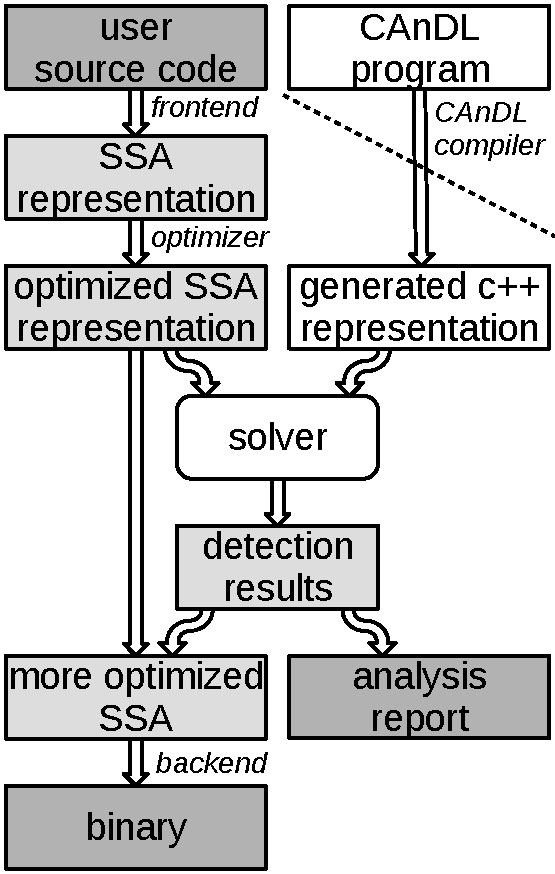
\includegraphics[width=0.59\textwidth]{figures/compilerFlow2.pdf}
\caption{CAnDL in the LLVM/Clang system: The CAnDL code gets parsed by the
         CAnDL compiler and turned into C++, which is compiled directly
         into LLVM and then used by Clang.
         \parfillskip=0pt}
\label{fig:build2}
\end{figure}

\section{Implementation}

    CAnDL is embedded in the LLVM framework, as shown in \Cref{fig:build2}.
    CAnDL programs are read by the CAnDL compiler during LLVM build time, which
    then generates C++ source code to implement the specified LLVM analysis
    functionality.
    This code depends on the generic backtracking solver derived in
    \Cref{chapter:theory}, which is incorporated directly into the LLVM code
    base.
    The generated code is compiled and linked together with the existing LLVM
    libraries.
    The Clang compiler, which is built on LLVM, then automatically invokes this
    solver during the compilation of user programs, after the standard
    optimisation passes.
    The evaluation at the end of the chapter will show that this solver adds
    little compile-time overhead in practice.

    The resulting modified version of the Clang compiler uses the solver to
    search for the specified computational structures and outputs the found
    instances into report files.
    It also makes the results available to ensuing transformation passes in the
    form of C++ structures.

\subsection{The CAnDL Compiler}

\begin{figure}[t]
\centering
\begin{minipage}{0.7\textwidth}
\centering
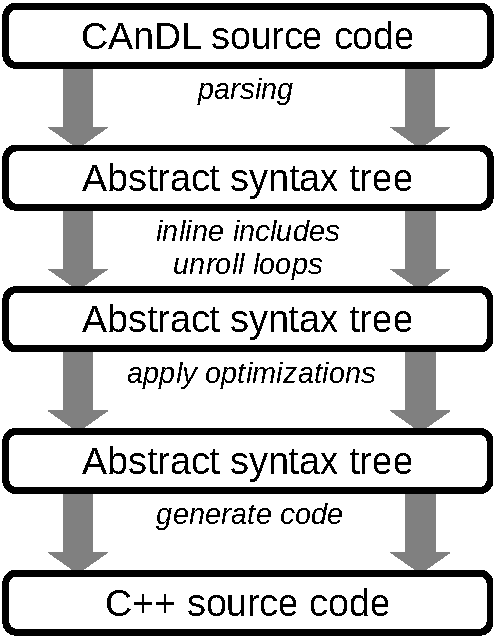
\includegraphics[width=0.85\textwidth]{figures/candlstages.pdf}
\caption{Flow within the CAnDL compiler:
         The CAnDL source code gets lowered in several steps to generated C++
         source code.\parfillskip=0pt}
\label{fig:compilerflow}
\end{minipage}
\end{figure}

    The CAnDL compiler is responsible for parsing CAnDL programs and
    generating C++ code from them.
    An overview of its  flow is shown in \Cref{fig:compilerflow}.
    The frontend reads in  CAnDL source code and builds an abstract syntax tree.
    This syntax tree is simplified in two steps to eliminate some of the higher
    order constructs of CAnDL.
    The {\it inheritance} clauses are inlined after the contained variables
    have been transformed accordingly.
    Also, {\it foreach} and {\it forany} statements are lowered to
    conjunction and disjunction constructs by duplicating the contained
    constraint code and then renaming its variables appropriately
    for each iteration.
    The remaining core language now consists only of atomics, conjunctions,
    disjunctions and collections.

    The CAnDL compiler then applies a set of optimisations to speed up the
    solving process using the later generated C++ code.
    For example, nested conjunctions and disjunctions are flattened wherever
    possible.
    Furthermore, if shallow equivalence of two variables is enforced in a
    conjunction, one of the two variables is chosen as having higher priority.
    all occurrences of the other variable are then replaced with that one.

    Finally, the compiler generates C++.
    This essentially means generating a function which at runtime constructs
    the constraint problem as a graph structure that is accessible to the
    solver.

\subsubsection{C++ Code Generation}

\begin{figure}[t]
\centering
\begin{lstlisting}[language=CAnDL]
Constraint SimpleAddition
( opcode{addition} = add
∧ {addition}.args[0] = {left}
∧ {addition}.args[1] = {right}) End
\end{lstlisting}
\begin{lstlisting}[language=MyCpp,label={fig:codegen},caption=
   {C++ code generation: The code is generated to first instantiate atomic
    constraints, then compose higher-level constructs and finally assemble a
    backtracking solution for the solver.\parfillskip=0pt}]
// Step 1: Instantiate Atomic Constraints
auto constr0 = make_shared<AddInstruction>(model);
auto constr1 = make_shared<FirstArgument> (model);
auto constr2 = make_shared<SecondArgument>(model);
// Step 2: Compose Higher-Level Constraints
auto constr3 = make_shared<Conjunction>(
                   constr0,
                   select<0>(constr1),
                   select<0>(constr2));
// Step 3: Assemble Backtracking Solution
vector<pair<string,shared_ptr<BacktrackingPart>>> result(3);
result[0] = make_pair("addition", constr3);
result[1] = make_pair("left",     select<1>(constr1));
result[2] = make_pair("right",    select<1>(constr2));
\end{lstlisting}
\end{figure}

    The code generation process is demonstrated with an example in
    \Cref{fig:codegen}.
    Every atomic constraint in CAnDL results in a line of C++ code that
    constructs an object of a corresponding class:
    In this case, the three involved atomic constraints are implemented by
    \texttt{AddInstruction}, \texttt{FirstArgument} and \texttt{SecondArgument}.
    These objects are instantiated as shared pointers.

    The compiler then generates similar objects for the
    \texttt{conjunction}, \texttt{disjunction} and the \texttt{collect} structures.
    In our example, this only affects the variable \texttt{addition}, which is
    part of a \texttt{conjunction} clause.
    This results in an additional object construction that instantiates the
    \texttt{Conjunction} class corresponding to the ``$\land$'' operator
    in CAnDL.

    Those constraint classes that implement constraints on a single variable
    directly implement the \texttt{BacktrackingPart} interface introduced in
    \Cref{cppsolver}.
    In the example, this applies to \texttt{AddInstruction} and
    \texttt{Conjunction}.
    For more complex constraints, the \texttt{select<n>} template is used to
    specify which variable of a constraint is being considered.
    In lines 6--7, this is used to extract the parts of backtracking solutions
    referring to the \texttt{addition} variable, and to then pass them as
    arguments to the conjunction.

    Finally, the generated objects are inserted into a vector, together with the
    corresponding variable names.
    The variables are in the order of appearance in the CAnDL code.
    This vector corresponds to the backtracking solution of the constraint
    problem and is passed to the solver.

\begin{figure*}[ht]
\centering
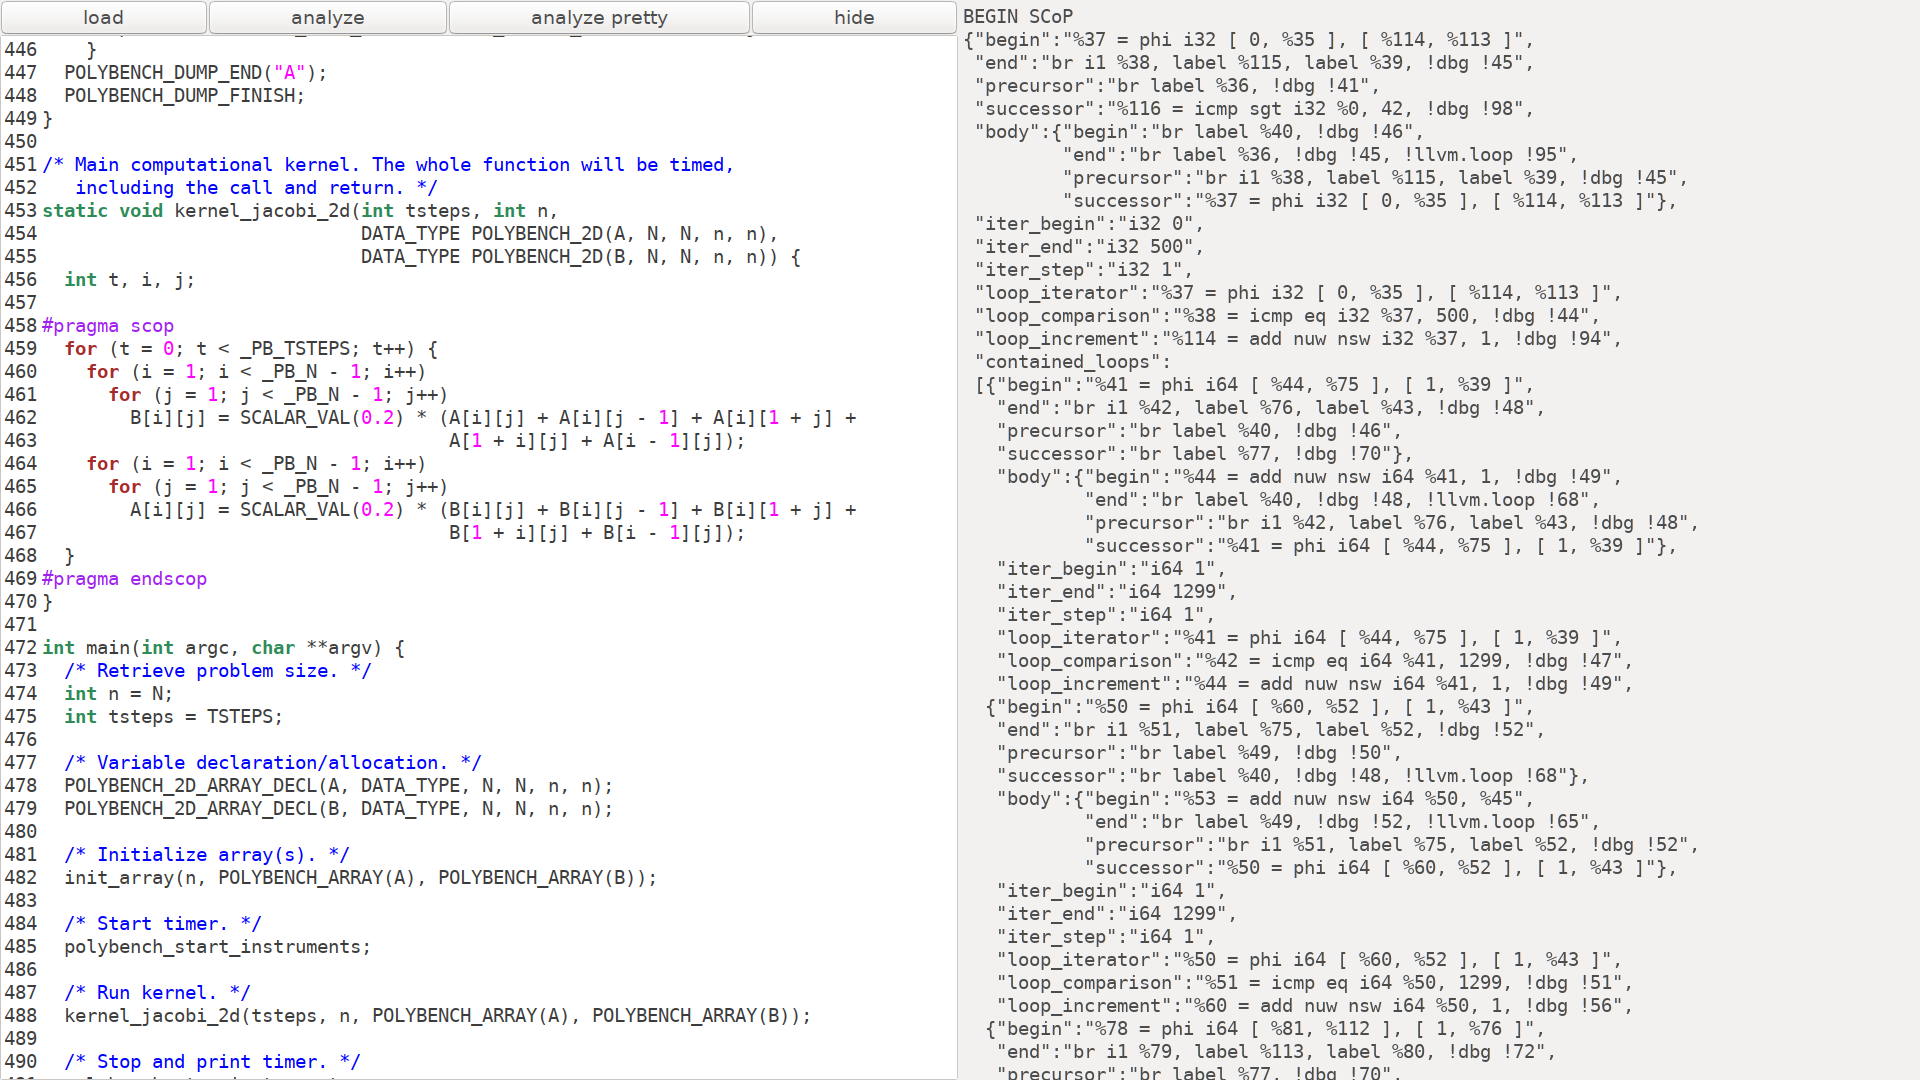
\includegraphics[width=0.98\textwidth]{figures/visual_gui2.png}
\caption{Interactive CAnDL test tool: The left hand panel shows a static control
        part (SCoP) in Polybench jacobi-2d, the right hand panel shows the
        constraint solutions found by the solver.
        \parfillskip=0pt}
\label{fig:gui}
\end{figure*}

\subsection{Developer Tools}

    CAnDL simplifies the construction of compiler analysis functionality
    drastically, but reasoning about the semantics of compiler intermediate
    representation still remains difficult.
    The solver detects whatever the programmer specifies, without any additional
    effort, but it is difficult to ascertain that the CAnDL code actually
    specifies the structures that the programmer intended.
    Generally, the correctness of CAnDL programs can only be guaranteed with
    thorough testing, and it is important to keep in mind that CAnDL is targeted
    at expert compiler developers.

    In order to make the debugging of CAnDL programs more feasible, 
    supporting tools are provided.
    Most importantly, this includes an interactive GUI, where developers can
    test out corner cases of their CAnDL programs to find false positives and
    false negatives.
    This GUI is shown in \Cref{fig:gui}, with an example from one of the use
    cases presented in \Cref{sec:casestudies}.

    In the left half, part of a C program from the PolyBench benchmark suite
    is visible, which implements a two-dimensional Jacobi stencil.
    The GUI was configured to look for static control regions (SCoPs), as
    described later.
    The user has clicked the ``analyze'' button, which triggered the analysis to
    run by invoking the modified Clang compiler.
    The GUI then read the report file, and printed the results in the right
    hand part of the figure.

    The solver found a SCoP in the IR code (corresponding to lines 459-468 of
    the C program).
    The text on the right shows the hierarchical structure of the solution, with
    IR values assigned to every variable.
    The corresponding C entities can be recovered using the debug
    information that is contained in the generated LLVM IR code.
    By modifying the C code, the developer can now test the detection and
    e.g.\ verify that no SCoP is detected if irregular control flow is
    introduced.

\section{Case Studies}
\label{sec:casestudies}

    The usefulness of CAnDL was evaluated with three different use cases.
    Firstly, it was used for detecting opportunities to apply a simple peephole
    optimisation.
    Secondly, CAnDL was applied to graphics shader code optimisation.
    Finally, the detection of static control flow parts (SCoPs) that are
    amenable for polyhedral code transformations was implemented in CAnDL.
    Where possible, the evaluation compares the number of lines of CAnDL code,
    the achieved program coverage and performance against prior approaches.

\subsection{Case Study 1: Simple Optimisations}

\begin{figure}[t]
\begin{lstlisting}[language=CAnDL,label={fig:facopport},caption=
   {Factorisation opportunities in CAnDL: This captures some opportunities that
    LLVM {\tt instcombine} misses. {\tt SumChain} and {\tt MulChain} are
    themselves specified in CAnDL (16 LoC).}]
Constraint ComplexFactorisation
( opcode{value} = add
∧ {sum1.value} = {value}.args[0]
∧ {sum2.value} = {value}.args[1]
∧ include SumChain @ {sum1}
∧ {product1.value} = {sum1.last_factor}
∧ include MulChain @ {product1}
∧ {product1.last_factor} = {product2.last_factor}
∧ include SumChain @ {sum2}
∧ {product2.value} = {sum2.last_factor}
∧ include MulChain @ {product2}) End
\end{lstlisting}
\end{figure}

    Arithmetic simplifications in LLVM are implemented in the
    \texttt{instcombine} pass.
    One example of this is the standard factorisation optimisation that uses the
    law of distributivity to simplify integer calculations as shown in
    \Cref{fig:factorization1}.
    Within {\tt instcombine}, this is implemented in 203 lines of code, and
    furthermore uses supporting functionality that is shared with other peephole
    optimisations.
    \begin{align}
        a*b+a*c\rightarrow a*(b+c)
        \label{fig:factorization1}
    \end{align}

    This analysis problem can be formulated in CAnDL as shown in
    \Cref{fig:facopport}.
    Crucially, in lines 5,7,9,11, the specification makes use of
    \texttt{SumChain} and \texttt{MulChain}, which allows the CAnDL program
    to capture a large, generalised class of opportunities for factorisation.
    The \texttt{instcombine} pass only has limited support for this, and
    requires to first apply associative and commutative laws to reorder the
    values.
    For example, this is needed for the constellation in
    \Cref{fig:factorization2}, and only partially supported by LLVM with the
    additional \texttt{reassociate} pass.
    \begin{align}
        a*b+c+d*a*e->a*(b+d*e)+c
        \label{fig:factorization2}
    \end{align}

\subsubsection{Setup}

    The specification in \Cref{fig:facopport} was evaluated against the default
    factorisation optimisation in \texttt{instcombine} on three different
    benchmark collections:
    The sequential C versions of the NAS Parallel Benchmarks
    \citep{Bailey1991NPB}, as provided by \citet{seo2011performance};
    the C/C++ Parboil benchmarks from \citet{stratton2012parboil};
    and the OpenMP C/C++ programs of the Rodinia benchmark suite
    \citep{Che2009Rodinia}.
    The existing LLVM \texttt{instcombine} pass was extended, so that it
    automatically reports every time that it successfully applies the
    \texttt{tryFactorization} function.  

    % NPB:     29047 loc
    % Parboil:  7358 loc
    % Rodinia: 58510 loc
    The individual benchmark programs in the three benchmark
    suites consist of 94915 lines of code in total.
    For each benchmark suite, the total number of reported factorisations as
    well as the total compilation time were measured.

    The standard LLVM optimisation was then disabled, and the CAnDL generated
    detection functionality was used instead.
    The same application programs were compiled with the same version of Clang
    and identical compiler options, reporting the number of factorisations
    found, and again measuring the total compilation time.
    Note that this compilation time includes all the other passes within LLVM
    plus the CAnDL generated code path.

\subsubsection{Results}

\begin{table}[t]
\centering
\begin{tabular}{|l||l|l|}
\hline
         & LLVM  &CAnDL \\
\hline
\hline
Lines of Code & 203 & 12 \\
\hline
Detected in NPB & 1 & 1 + 2 \\
Detected in Parboil & 0 & 0 + 1\\
Detected in Rodinia & 24 & 24 + 4\\
\hline
Total Compilation time & 152.2s & 152.2s+7.8s \\
\hline
\end{tabular}
\caption{Factorisations enabled by LLVM vs CAnDL}
\label{fig:factorization_results}
\end{table}

    The results of the evaluation are shown in
    \Cref{fig:factorization_results}.
    In two of the benchmark collections -- NPB and Parboil -- there are
    only a limited number of factorisation opportunities.
    LLVM was unable to perform any factorisation in the entire Parboil suite.
    However, the Rodinia suite contains more opportunities, mostly in the
    Particlefilter and Mummergpu programs.

    In all three benchmarks suites, the CAnDL system found all the factorisation
    opportunities that the \texttt{instcombine} pass identified.
    In addition, it detected an additional 7 cases across all programs.
    Only 12 lines of CAnDL code were able to capture more factorisation
    opportunities than LLVM did using two hundred lines of code.

    Using CAnDL on large benchmark suites only increased total compilation time
    by \mbox{$\sim5\%$}.
    Given the generally small impact of individual peephole optimisations, an
    evaluation of the performance or code size impact vs {\tt instcombine} is
    unlikely to yield significant results.

\subsection{Case Study 2: Graphics Shader Optimisations}

\begin{figure}[t]
\begin{lstlisting}[language=CAnDL,label={fig:Lewis},caption=
   {CAnDL defines multiplication chains involving genuine vectors and hoisted
    scalars:
    After separating the two cases, some of the multiplications can be performed
    on scalars instead.\parfillskip=0pt}]
Constraint FloatingPointAssociativeReorder
( include VectorMulChain
∧ collect j N
∧ ( {hoisted[k]} = {factors[i]} forany i=0..N
  ∧ include ScalarHoist({hoisted[j]}->{out},
                       {scalar[j]}->{in})@{hoist[j]})
∧ collect j N
  ( {nonhoisted[j]}  = {factors[i]} forany  i=0..N
  ∧ {nonhoisted[j]} != {hoisted[i]} foreach i=0..N))
End
\end{lstlisting}
\end{figure}

    Graphics computations often involve arithmetic on vectors of single
    precision floating point values, which can represent either vertex positions
    in space or colour values.
    Common graphics shader compilers utilise the LLVM framework internally.
    The LunarGLASS project \citep{lunarglass} was used in this work as an open
    source implementation of LLVM for graphics shaders.

    In real shader code, there are often element wise products of multiple
    floating point vectors, where several of the factors are actually scalars
    that were hoisted to vectors.
    By reordering the factors and delaying the hoisting to vectors, some of the
    element wise vector products can be simplified to products on scalars, as
    shown by example in the following equation.
    \begin{align*}
        \vec x={}&\vec a*_v\vec b*_v\text{vec3}(c)*_v\vec d*_v\text{vec3}(e)\\
        ={}&\text{vec3}(c*e)*\vec a*_v\vec b*_v\vec d
    \end{align*}

    For general purpose code, such reordering can be problematic.
    This is due to computation artefacts in floating point arithmetic.
    However, this is not a problem in the domain of graphics processing.
    Instead, associative reordering can result in real performance improvements
    when combined with lowering to scalar multiplications as discussed above.

    The required analysis functionality for this optimisation was implemented
    with CAnDL, as shown in \Cref{fig:Lewis}.
    Firstly, the specification includes \texttt{VectorMulChain} to detect 
    chains of floating point vector multiplications.
    In lines 4--6, all the factors that are hoisted from some scalar are
    collected into the array {\tt hoisted}.
    Correspondingly, all the other factors are collected into the array
    {\tt nonhoisted} in lines 7--9.

    {\tt VectorMulChain} and {\tt ScalarHoist} are themselves implemented as
    CAnDL programs.
    {\tt VectorMulChain} discovers chains of floating point vector
    multiplications in the IR code.
    It is defined very similarly to {\tt SumChain} and {\tt MulChain}, which
    were used in the previous case study.
    It guarantees chains of maximal length by checking that neither of the first
    two factors is a multiplication itself, and that the last factor is not used
    in any multiplication.
    \texttt{ScalarHoist} operates on the variables {\tt in} and {\tt out}, as
    well as some internals.
    It specifies that {\tt out} is a vector generated from {\tt in} by setting
    all vector dimensions to the value of {\tt in}.
    The implementation of this is very specific to LLVM and involves
    combinations of the LLVM IR instruction {\tt insertelement} and
    {\tt shufflevector}

\subsubsection{Setup}

    The CAnDL specification was applied to all fragment shaders in the
    GFXBench 4.0 suite from \citet{gfxbench}.
    A corresponding transformation pass was added to LLVM, which uses the
    detected solutions to implement the described optimisation.
    This is done by constructing the appropriate scalar and vector
    multiplications from the arrays {\tt hoisted} and {\tt nonhoisted}, and then
    replacing the result of the original vector multiplication chain with the
    final multiplication in these newly generated instructions.
    Standard dead code elimination automatically removes the remnants of the
    original calculation.

    The performance impact was evaluated on the Qualcomm Adreno 530 GPU.
    To measure the baseline of benchmark performance, all shaders were
    compiled with the default Qualcomm graphics stack.
    They were then compiled with LunarGLASS, and the resulting LLVM IR was
    optimised using CAnDL.
    To evaluate the impact of this, the result was again passed through the
    default graphics stack and the performance of the benchmarks measured.

\subsubsection{Results}

\begin{figure}[t]
\centering
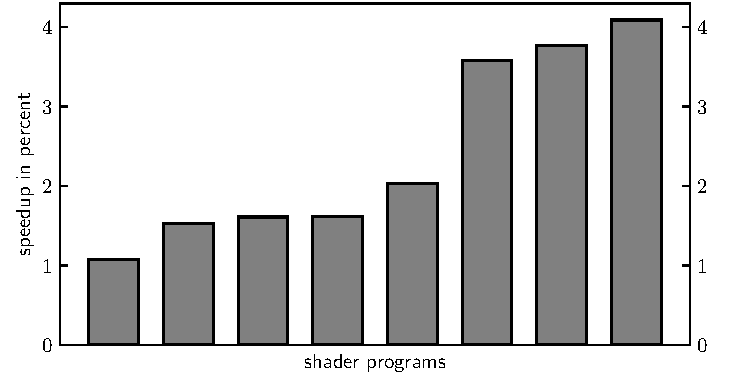
\includegraphics[width=0.66\linewidth]{figures/qualcomm_plot.pdf}
\caption{Speedup on Qualcomm Adreno 530}
\label{fig:qualcommspeedup}
\end{figure}

%\begin{figure}[b]
%\centering
%\begin{tabular}{|l||l|l|}
%\hline
%         & LLVM  &CAnDL \\
%\hline
%\hline
%Lines of Code & Not implemented& 10 \\ \hline
%Detected in GFX 4.0 & - & 19 \\ \hline
%\hline
%\end{tabular}
%\caption{Shader optimization LLVM vs CAnDL}
%\label{fig:candlshader}
%\end{figure}

    There were 19 solutions to the specification across the benchmarks, and
    the transformation had an impact on the performance of 8 fragment shaders.
    The resulting performance impact is shown in \Cref{fig:qualcommspeedup}.
    Evidently, there are opportunities for such associative reordering that
    the default graphics stack misses.
    Although the performance impact was moderate with 1--4\% speedup on eight
    of the fragment shaders, it shows how new analysis can be rapidly prototyped
    and evaluated with only a few lines of code.

\subsection{Case Study 3: Detection of Polyhedral SCoPs}

    The polyhedral model allows compilers to utilise powerful mathematical
    reasoning to detect parallelism opportunities in sequential code and to
    implement code transformations for well structured nested
    loops.
    Conventional polyhedral code transformations are applicable to
    static control parts (SCoPs).
    These are regions of code that comprise nestings of well-behaved loops and
    conditionals with only affine data access patterns inside.
    Detecting SCoPs is fundamental and necessary first step for any later
    polyhedral optimisation.

    Implementations of the polyhedral model may differ in their precise
    definition of SCoPs.
    In this work, the definition of Semantic SCoPs from
    \citet{Lengauer2012Polly} was used for reference.
    SCoP detection functionality was implemented in CAnDL and compared against
    Polly \citep{Lengauer2012Polly}, which is a polyhedral compiler that is
    implemented as an extension to LLVM.
    The use of the same definition for SCoPS and the implementation in the same
    compiler infrastructure allow for a direct comparison between Polly and
    CAnDL.
    The specification of SCoPs is significantly more complex than the required
    CAnDL code for the previous case studies.
    However, it can be broken into several components
    \footnote{The complete CAnDL code for this section can be found in
    Appendix~\ref{appendix:CAnDLpoly}.}.

    \paragraph*{Structured Control Flow}
    SCoPs require well structured control flow.
    Technically speaking, this means that every conditional jump within the
    corresponding piece of IR is accounted for by for loops and conditionals.
    This is enforced with the \texttt{collect} statement that was introduced in
    \Cref{fig:collectexample}.
    It is used in CAnDL programs \texttt{ForLoop} and
    \texttt{Conditional} that describe the control flow of for loops and
    conditionals and extract the involved conditional jump instructions.
    Another \texttt{collect} is then used to verify that these are indeed all
    conditional jumps within the potential SCoP.

    Once the control flow has been established, the iterators that are
    involved in the loops are used to define affine integer computations in the
    loop.
    This is done in a brute force fashion with a recursive constraint program.
    Using this analysis we then check that the iteration domain of all the for
    loops is well behaved, i.e.\ the boundaries are affine in the loop
    iterators.

    \paragraph*{Affine Memory Access}
    All memory access in the SCoP has to be affine.
    For this to be true, it needs to be verified that for each load and store
    instruction, the base pointer is loop invariant and the index is calculated
    affinely.
    The loop invariant base pointer is easily guaranteed using the
    \texttt{LocalConst} program from \Cref{localconstant}.

    Checking the index calculations is more involved and is again based on the
    \texttt{collect} method that was demonstrated in \Cref{fig:collectexample}.
    The \texttt{collect} construct is used to to find all of the affine memory
    accesses in all the loop nests.
    We then use collect all \texttt{load} and \texttt{store} instructions and
    verify that both collections are identical.

\pagebreak
\phantom{placeholder}
\pagebreak

\subsubsection{Setup}

    The reliable detection of SCoPs was evaluated on the PolyBench suite by
    \citet{polybench}.
    For both the CAnDL based approach as well as for Polly, it was counted
    counted how many of the computational kernels contained in the benchmark
    suite were captured by the analysis.

    Some post-processing of the generated constraint solutions was required to
    compare the results of CAnDL and Polly.
    This is because the CAnDL results are not in the {\it jscop} format that
    Polly uses, but contain instead the raw constraint solution.
    Also, the CAnDL implementation does not merge consecutive outer level loops
    into a single SCoP of maximum size.
    Therefore, the detected loops from the CAnDL solver were extracted and then
    grouped together, after which it was manually verified whether they
    precisely cover the SCoPs detected by Polly.

\subsubsection{Results}

    \Cref{fig:candlvspolly} shows that the CAnDL specification captured all the
    SCoPs that Polly detected.
    To measure lines of code, the CAnDL version was compared with the amount of
    code in \texttt{ScopDetection.cpp} of Polly.
    The same detection results were achieved with much fewer lines of code in
    CAnDL.
    Note that the line count that is given for the CAnDL program does not
    include all the CAnDL code involved in the detection of polyhedral regions.
    Code that is not specific to this idiom (such as loop structures) are
    considered as part of the CAnDL standard library.
    In the same way, the line count for Polly does not account for additional
    code that Polly relies on when detecting SCoPS, e.g\ the expansive
    ScalarEvolution pass.

    By having a high level representation of SCoPs, we allow polyhedral compiler
    researchers to explore the impact of relaxing or tightening the exact
    definition of SCoPs in a straightforward manner, enabling rapid prototyping.

\begin{table}[ht]
    \centering
\begin{tabular}{|l||l|l|}
\hline
         & Polly & CAnDL \\
\hline
\hline
Lines of Code & 1903 & 45 \\ \hline
Detected in datamining & 2 & 2\\
Detected in Linear-algebra & 19 & 19\\
Detected in medley & 3 & 3\\
Detected in stencils & 6 & 6\\ \hline
%Compilation time & 24.4s+37.5s & 24.4s+12.7s \\ \hline
\end{tabular}
    \caption{SCoPs detected Polly vs CAnDL}
    \label{fig:candlvspolly}
\end{table}

\pagebreak

\section{Summary}

    Optimising compilers require sophisticated program analysis in order to
    generate performant code.
    The current way of implementing this functionality manually in programming
    languages such as C++ is not satisfactory, as exemplified by the overly
    complex {\tt instcombine} pass in the LLVM compiler infrastructure.

    The domain specific Compiler Analysis Description Language (CAnDL) provides
    a more efficient approach.
    CAnDL programs can be used to automatically generate compiler analysis
    passes.
    They are easier to write and significantly reduce the code size and
    complexity when comparing against manual C++ implementations.

    Although CAnDL is based on a constraint programming paradigm and uses a
    backtracking solver to analyse LLVM IR code, the use of it results in
    only moderate compile time increases.
    Many compiler analysis tasks are suitable for implementation with CAnDL,
    from detecting peephole optimisation opportunities to recognising large
    code regions that are suitable for analysis with the polyhedral model.


\chapter[Automatic Parallelisation of Complex Reductions and Histograms]
        {Automatic Parallelisation of Complex Reductions and Histograms
         \footnote{This chapter is based on published research in
                   \citet{ginsbach2017discovery}.}}
    \label{chapter:reductions}
    
    The Compiler Analysis Description Language (CAnDL) makes the constraint
    methodology from \Cref{chapter:theory} accessible to the Clang compiler
    within the LLVM compiler infrastructure.
    The previous chapter showed how this enables compiler analysis tools to be
    generated from declarative specifications, replicating and extending
    established compiler abilities.
    This chapter goes beyond restating and improving existing functionality.
    Instead, it implements automatic parallelisation methods for programs that
    were previously inaccessible to compiler reasoning.

    Complex Reduction and Histogram Computations (CReHCs) are identified as a
    previously overlooked  {\em computational idiom}.
    CReHCs constitute performance bottlenecks of important benchmark programs
    and share algorithmic structure that allows for targeted acceleration and
    parallelisation approaches.
    In contrast to the better-understood scalar reductions, CReHCs may contain
    indirect memory accesses and non-trivial control flow.
    Such loops have not typically been studied as a single class of
    calculations, but this chapter demonstrates that grouping them together
    allows for automatic detection and parallelisation using shared methods.

    After introducing CReHCs, this chapter presents the Idiom Description
    Language (IDL) as an extension of CAnDL and uses it to implement the
    detection of this idiom.
    The additional language features of IDL enable capturing well-behaved
    kernel functions.
    CReHCs contain reduction operators that are modelled as kernel functions,
    but kernel functions are also required in the formulation of other
    computational idioms, such as stencil codes.
    
    Grouping reductions and histograms together and formulating CReHCs in IDL
    enables their automatic recognition in C/C++ program code.
    The evaluation section shows results from benchmarking the outcomes of
    parallelisation routines that were implemented to complement the detection.
    Significant speedups were achieved on several programs from the
    NAS Parallel Benchmark suite, the Parboil Benchmarks, and Rodinia.

\section{Introduction}

    Reductions occur widely in numerical applications.
    Parallelisation techniques for them were established by
    \citet{rauchwerger1999lrpd,yu2006adaptive,Jradi2017fast}, and others.
    Typical reductions successively apply an arithmetic operator over an
    array of numeric values in order to compute, for example, the sum of a set
    of floating-point numbers.
    Perhaps most prominently, a reduction makes up the innermost loop of the
    matrix multiplication kernel in the form of a dot product.
    In this form, reductions are critical to high performance computing
    workloads based on linear algebra, as well as embedded benchmarks and
    emerging machine learning and computer vision applications
    \citep{Reddy2016Reduction}.
    Even so, linear algebra allows for much more targeted optimisation methods.
    Interpreting the innermost loop of matrix multiplication as an arbitrary
    reduction is unlikely to achieve comparable performance.

    However, there is a much larger class of computations that can be
    parallelised in much the same way.
    This is the class of Complex Reduction and Histogram Computations (CReHCs),
    a broad generalisation of conventional reductions that may also contain
    updates to dynamically selected elements in arrays.
    This manner of array access is characteristic for the calculation of
    histograms.
    CReHCs constitute an important set of standard program kernels.
    They typically have a higher arithmetic intensity and can be more profitably
    exploited on their own than simple scalar reductions.

    Discovering and exploiting scalar reductions in programs has been
    studied for many years, by \citet{pottenger1995idiom}, among others.
    The treatment of generalisations of reduction operations has received less
    attention.
    While some work has been published on parallelising such computations,
    automatic detection mostly evades established compiler analysis methods.
    The reason is that histogram reductions intrinsically contain indirect
    memory accesses, posing a challenge to compilers that use
    standard data dependence \citep{kuck1981dependence} or the polyhedral model
    \citep{benabderrahmane2010polyhedral} as the basis of their analysis.

    The constraint programming methodology derived in \Cref{chapter:theory},
    however, is not inhibited by such indirect memory accesses.
    \Cref{chapter:candl} developed the constraint programming language CAnDL
    using this methodology and showed that it could also recognise intricate
    control flow.
    This chapter presents the Idiom Detection Language (IDL) as an extension
    of CAnDL and uses it to implement the detection of CReHCs.
    The additional language features enable IDL to express well-behaved
    kernel functions, which capture the reduction operators of CReHCs.
    The IDL solver automatically identifies conforming subsets of LLVM IR during
    compilation.

    This chapter focuses on deriving the detection of reductions and assumes
    that later compiler stages are responsible for mapping this to dedicated
    code generation backends.
    Nonetheless, to illustrate the potential performance of the scheme, it uses
    also introduces a complementing code generation pass.
    This transformation pass achieved significant program-wide speedups on those
    benchmarks where reductions were performance bottlenecks.

\section{Motivation}

    \Cref{sum-figure} shows a standard scalar reduction.
    Inside a single loop, the elements of the array ``\texttt{a}'' are
    successively accumulated in the variable ``\texttt{sum}'' using the
    ``\texttt{+=}'' operator.
    This accumulation creates dependencies between successive loop iterations.
    However, those are easy to break.
    Rather than sequentially accumulating ``{\tt a}'' into ``{\tt sum}'', it is
    possible to accumulate partial sums into thread-private copies of
    ``\texttt{sum}'' in parallel, which are then added to form the final value.

\begin{figure}[h]
\begin{lstlisting}[language=MyCpp, label={sum-figure}, caption=
    {The most conventional example of a reduction is the adding up of values
     in an array:
     The reduction operator ``{\tt+}'' {\it reduces} the array ``\texttt{a}'' to
     a single value -- the reduction variable ``{\tt sum}''.}]
sum = 0;
for(i = 0; i < n; i++)
  sum += a[i];
\end{lstlisting}
\end{figure}

    Simple scalar reductions frequently occur, and existing compilers readily
    exploit them.
    Despite their abundance, scalar reductions rarely dominate execution time,
    and when they do, they are often part of more prominent algorithms, such as
    matrix multiplication.
    This often makes outer-scope parallelism more profitable to exploit.
    Therefore, the parallelisation of simple reductions alone has only a
    limited impact on program performance.

    \Cref{complex-reduction-figure} shows a more complex section of code that
    constitutes a performance bottleneck of the ``Embarrassingly Parallel''
    benchmark program in the NAS Parallel Benchmarks.
    Note that the name of the benchmark refers to outer-loop parallelism.
    It is not directly evident that this computation can be treated as a
    reduction.
    However, it can be parallelised similarly to the simple sum.
    Creating thread-private copies of the reduction variables is again the
    critical step.

\begin{figure}[h]
\begin{lstlisting}[language=MyCpp, label={complex-reduction-figure}, caption=
   {Example of a Complex Reduction and Histogram Computation:
    The bottleneck from the NAS Parallel Benchmarks can be parallelised as a
    reduction by privatising ``\texttt{sx}'', ``\texttt{sy}'',
    ``\texttt{q[]}''.}]
for(i = 0; i < NK; i++) {
  x1 = 2.0 * x[2*i] - 1.0;
  x2 = 2.0 * x[2*i+1] - 1.0;
  t1 = x1 * x1 + x2 * x2;
  if(t1 <= 1.0) {
    t2   = sqrt(-2.0 * log(t1) / t1);
    t3   = (x1 * t2);
    t4   = (x2 * t2);
    l    = MAX(fabs(t3), fabs(t4));
    q[l] = q[l] + 1.0;
    sx   = sx + t3;
    sy   = sy + t4;
  }
}
\end{lstlisting}
\end{figure}

    The loop in \Cref{complex-reduction-figure} is considered a CReHC for the
    following reasons:
    Firstly, there is an input array ``\texttt{x[]}'', from which values are
    read successively in each iteration.
    Secondly, the values ``\texttt{sx}'' and ``\texttt{sy}'' are scalar
    reduction variables, as is evident from lines 11--12.
    They are incremented conditionally, and the added value is not merely
    ``\texttt{x[i]}'' but the result of a complex calculation with control flow.
    Nonetheless, the calculation and the branching condition only depend on the
    input values ``\texttt{x[2*i]}'' and ``\texttt{x[2*i+1]}''.
    Thirdly, the array ``\texttt{q[]}'' is updated as a histogram array at
    line 10.
    The index ``\texttt{l}'' is not directly read from an input array, as in a
    conventional histogram, but again the calculation only depends on the input
    values.

    As in the case of the simple sum, the parallelisation of this code
    requires the computation of partial results in separate memory locations
    before merging the partial results.
    The whole process is illustrated in Figure \ref{nice-picture}, with
    different colours on the right showing the distribution of the program
    over two threads.
    The scalar variables ``\texttt{sx}'', ``\texttt{sy}'' and the array
    ``\texttt{q[]}'' are privatised.
    Partial results are then accumulated in the local copies by partitioning the
    input array equally across the two threads. 
    Finally, the threads are synchronised, and partial results merged.
    This is done by adding the local copies of ``\texttt{sx}'', ``\texttt{sy}''
    and performing an element-wise addition of the local copies of
    ``\texttt{q[]}''. 

\begin{figure}[t]
\centering
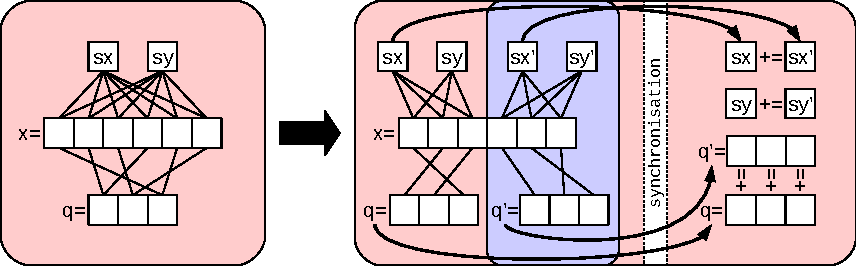
\includegraphics[width=\textwidth]{figures/parallelisereduction.pdf}
\caption{Parallelisation of \Cref{complex-reduction-figure}:
         The input ``\texttt{x[]}'' is split over two threads (red/blue)
         that operate on private copies of ``\texttt{sx}'', ``\texttt{sy}'',
         ``\texttt{q[]}''.
         These are merged after a synchronisation barrier.}
\label{nice-picture}
\end{figure}

\begin{figure}[p]
\centering
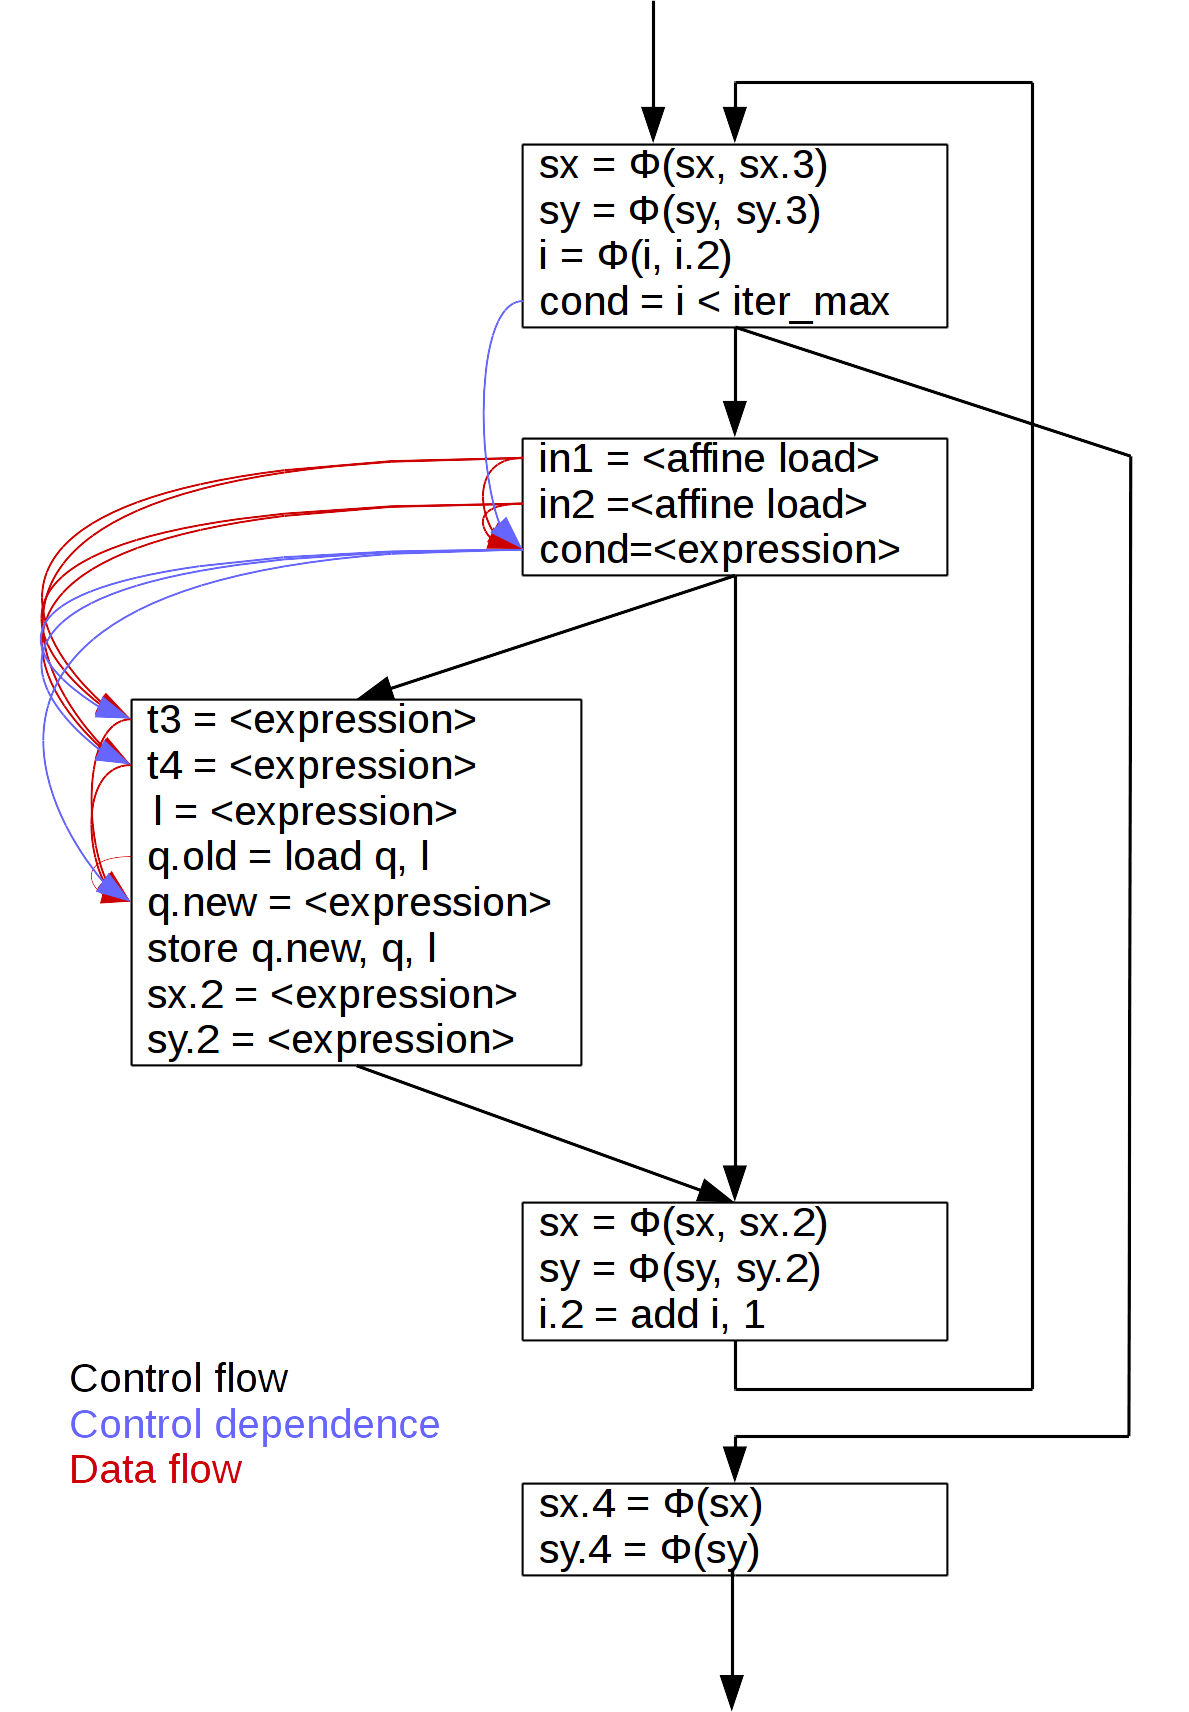
\includegraphics[width=\textwidth]{figures/nicepicture2.png}
\caption{Fragments of the data flow, control flow, and control dependencies in
         the internal compiler representation of the source code in
         \Cref{complex-reduction-figure}:
         These interactions must be considered when searching for code that
         implements Complex Reduction and Histogram Computations.}
\label{nice-picture2}
\end{figure}

    \Cref{nice-picture2} gives an insight into why existing schemes do not
    detect such reductions by showing the compiler representation of this 
    program.
    The histogram update occurs in the third basic block with the ``load'',
    assignment and ``store'' operations, but it is by no means obvious that this
    is a safe reduction.
    In fact, accurately detecting reductions is non-trivial.
    If in the original program, shown in \Cref{complex-reduction-figure}, the
    condition on line 5 was changed to ``{\tt t1 <= sx}'', this would be no
    longer be a sound reduction, as there would now be a control dependence on
    an intermediate result.
    This, in turn, would itself as an additional data dependence edge from
    block 3 to block 2 in \Cref{nice-picture2}.
    Furthermore, the code segment can only be classified as a reduction because
    all the function calls that are present are pure.
    Such details have to be checked to ensure correctness.
    What is needed is a way to specify these conditions precisely and to then
    automatically identify code regions that satisfy the constraints.

\section{Recognising CReHCs}

    There are three fundamental issues to address in exploiting CReHCs:
    detection, replacement, and profitability.
    This chapter focuses on the reliable detection of reductions.
    For evaluation purposes, a preliminary code generation phase that generates
    parallel code was implemented targeting the POSIX Threads interfaces.
    Smart profitability heuristics are essential in practice to determine
    whether or not to apply parallelising code transformations.
    For this work, a simple profile-based approach was used.

    In the following sub-sections, the properties that loops need to satisfy
    to be interpreted as CReHCs are derived.
    Conditions for sound CReHCs are established and demonstrated on
    counterexamples.
    These observations then motivate extensions to CAnDL that culminate in the
    Idiom Detection Language (IDL).
    This language eventually enables the constraint-based specification of
    CReHCs for automatic compiler detection.

\subsection{Constraint-Based Formulation}

    The motivation section described how CReHCs could be parallelised as
    reduction operations.
    For compilers to apply this parallelisation automatically, a precise
    specification of the suitable program loops is required.
    This section gives an overview of the necessary conditions for CReHCs, which
    are then precisely formulated in \Cref{sec:IDLdefinition,sec:IDLCReHCs}.

\subsubsection{Scalar Reductions}
\label{section:scalarcond}

    Informally, the following conditions are required to hold in a piece of
    source code for it to contain a computation that can be parallelised like a
    scalar reduction:
    \begin{enumerate}
        \item The code is contained in a for-loop, and the iteration space of
              the loop is known ahead of time
              (but not necessarily at compile time).
        \item There is a scalar value $x$ that is updated in every iteration.
        \item One or multiple values $a_1,\dots,a_n$ are read from arrays, and
              the access indices are affine in the loop iterator.
        \item The updated value $x'$ is computed as a term only of $x$, the
              array values $a_1,\dots,a_n$, and of values that are constant
              within the loop.
    \end{enumerate}

    This definition is broader than usual.
    In particular, it allows the reduction to encompass multiple input arrays.
    Furthermore, complex computations inside the reduction are possible, not
    just binary scalar operators.
    Note that condition 2 is enforced only at SSA level.
    Finally, this definition does not yet contain a commutativity condition that
    would be necessary to allow the parallelisation to work.
    Instead, it also captures intrinsically sequential scalar reductions.

    \paragraph*{Example}
    Both ``\texttt{sx}'' and ``\texttt{sy}'' in
    \Cref{complex-reduction-figure} satisfy the conditions.
    Firstly, the iteration space of the loop is bounded by ``\texttt{NK}'',
    which is constant.
    Secondly, within the SSA representation, both ``\texttt{sx}'' and
    ``\texttt{sy}'' are unconditionally updated via $\Phi$-instructions, shown
    in \Cref{nice-picture2}.
    This is despite the conditional statement in the original C representation
    of the program.
    Thirdly, two values are read from the single input array ``\texttt{x[]}''
    in every iteration, and the indices ``\texttt{2*i}'' and
    ``\texttt{2*i+1}'' are affine in ``\texttt{i}''.
    Finally, the updated values depend only on their respective old values,
    the two values read from ``\texttt{x[]}'', and the constants
    ``\texttt{1.0}'' and ``\texttt{2.0}''.
    This also relies on the fact that all functions used in the computation are
    pure functions.

\begin{figure}[t]
\begin{lstlisting}[language=MyCpp]
sum = 0;
for(i = 0; i < n && sum < 10; i++)
    sum += a[i];
\end{lstlisting}
\begin{lstlisting}[language=MyCpp]
sum = 0;
for(i = 0; i < n; i++)
    b[i] += a[i];
\end{lstlisting}
\begin{lstlisting}[language=MyCpp]
chase = 0;
for(i = 0; i < n; i++)
    chase = a[chase];
\end{lstlisting}
\begin{lstlisting}[language=MyCpp,label={counterexamples},caption=
   {Counterexamples to the four conditions: None of these computations can be
    parallelised as scalar reductions.
    The first and last example implement the same program.}]
sum = 0;
active = true;
for(i = 0; i < n; i++) {
    sum += active?a[i]:0;
    active = active && (sum < 10);
}
\end{lstlisting}
\end{figure}

    \paragraph*{Counterexamples}
    \Cref{counterexamples} shows counterexamples to the four conditions,
    demonstrating why they are all needed in order to parallelise a given
    computation as a scalar reduction.

    In the first example, the iteration space is not known in advance, as the
    computation can be terminated depending on the input data.
    This makes it impossible to compute partial sums in parallel.
    The second example is straightforward, as there is no reduction variable
    that could be privatised.
    The loop could still be computed in parallel -- but not as a scalar
    reduction.
    The third example uses index calculations that are not affine in
    ``\texttt{i}''.
    This prevents a straightforward distribution of the input array across
    threads.
    In this particular case, the index calculation also involves values other
    than ``\texttt{i}'', preventing the computation of partial results entirely.
    The final example is equivalent to the first but breaks the fourth condition
    instead of the first.

\subsubsection{Histogram Reductions}
\label{section:histocond}

    The conditions that apply to histogram reductions are similar to those for
    scalar reductions.
    However, instead of one function parameter, there are two:
    \begin{enumerate}
        \item The code is contained in a for-loop, and the iteration space of
              the loop is known ahead of time
              (but not necessarily at compile time).
        \item One or multiple values $a_1,\dots,a_n$ are read from arrays, and
              the access indices are affine in the loop iterator.
        \item An integer $k$ is computed as a term only of the array values
              $a_1,\dots,a_n$, and of values that are constant within the loop.
        \item A value $x$ is read from an array at index $k$ and a
              modified value $x'$ is written at the same index.
              The writing may be control-dependent only on $a_1,\dots,a_n$ and
              it may not be in a nested loop.
        \item The updated value $x'$ is computed as a term only of $x$, the
              array values $a_1,\dots,a_n$, and of values that are constant
              within the loop.
    \end{enumerate}

    Histogram reductions are only parallelisable if their update operator is
    commutative, just as is the case for scalar reductions.
    However, checking this condition requires a post-processing step,
    which is independent of the detection of the algorithmic structure.
    For this research, checking commutativity was considered the responsibility
    of code generation.

    \paragraph*{Example}
    The first two conditions are the same as those in the previous discussion of
    scalar reductions and were shown to hold for the loop in
    \Cref{complex-reduction-figure}.
    The array ``\texttt{q[]}'' also satisfies the remaining conditions.
    Firstly, the variable ``\texttt{l}'' corresponds to the index $k$.
    Secondly, the element ``\texttt{q[l]}'' is read, modified and written.
    Lastly, the updated value is computed in an allowed fashion, as it is
    obtained by merely adding a constant ``\texttt{1.0}'' to the previous value.

    \paragraph*{Counterexamples}
    Again, counterexamples are given in \Cref{counterexamples2} to develop an
    intuition about the significance of conditions 3--5.

    In the first example, the index of the histogram is not computed from an
    input array but instead read from an input stream.
    This makes parallelisation as a histogram impossible, as the stream is only
    available sequentially.
    In the second and third examples, the computation effectively stops when an
    index beyond a threshold size occurs.
    This can only be accounted for by sequentially going through the array.
    Therefore, the parallel computation of partial results is not efficiently
    possible.
    This behaviour is evoked in two different ways, by breaking the conditions
    4 and 5, respectively.
    This shows the need to restrict both the data flow and control flow of the
    histogram kernel.

\begin{figure}[t]
\lstset{
 basicstyle = \linespread{0.883}\ttfamily
}
\begin{lstlisting}[language=MyCpp]
for(i = 0; i < n; i++)
    hist[getchar()] += 1;
\end{lstlisting}
\begin{lstlisting}[language=MyCpp]
active = true;
for(i = 0; i < n; i++) {
    if(a[i] > 9)
        active = false;
    if(active)
        hist[a[i]] += 1;
}
\end{lstlisting}
\begin{lstlisting}[language=MyCpp,label={counterexamples2},caption=
   {Counterexamples to the last three conditions:
    None of these computations can be parallelised as histograms.
    The final two example loops implement equivalent functionality.}]
active = true;
for(i = 0; i < n; i++) {
    if(a[i] > 9)
        active = false;
    hist[a[i]] += active?1:0;
}
\end{lstlisting}
\end{figure}

\subsection{The Idiom Detection Language}
\label{sec:IDLdefinition}

    For automatic detection during compilation, the conditions from
    \Cref{section:histocond,section:scalarcond} are specified formally in
    a constraint language.
    CAnDL from \Cref{chapter:candl} is taken as the basis for this formulation.
    However, additional language constructs are required in order to capture
    the kernel computations.

    This extension of CAnDL leads to the definition of the
    Idiom Detection Language (IDL).
    IDL uses the solver infrastructure of CAnDL and retains the same high-level
    program structure.
    However, it extends the language and modifies the syntax to be more
    convenient for large-scale specifications, replacing uncommon Unicode
    characters.
    \Cref{CanDLtoIDL} shows syntax differences.\footnote{The complete grammar
    file that was used to generate the parser of the IDL compiler is in
    Appendix~\ref{appendix:IDLgrammar}.}

\begin{table}[H]
    \lstset{keepspaces}
    \centering
    \definecolor{tableShade}{gray}{0.8}
    \rowcolors{1}{}{tableShade}
    \begin{tabular}{p{0.39\textwidth}p{0.553\textwidth}}
        \toprule
        {\bf CAnDL} & {\bf IDL}\\
        \midrule
        {\lstinline[language=CAnDL]!∧!}, {\lstinline[language=CAnDL]!∨!} &
        {\lstinline[language=IDL]!and!}, {\lstinline[language=IDL]!or!} \\
        {\lstinline[language=CAnDL]!include Spec({A}->{B}!}, \vspace{-2.5mm}\newline
        {\phantom{\lstinline[language=CAnDL]!include Spec(!}\lstinline[language=CAnDL]!{C}->{D})@{E}!} &
        {\lstinline[language=IDL]!inherits Spec with {A} as {B}!} \vspace{-2.5mm}\newline
        {\phantom{\lstinline[language=IDL]!inherits Spec!}\hspace{4.4mm}\lstinline[language=IDL]!and {C} as {D} at {E}!}\\
        {\lstinline[language=CAnDL]!{A}={B}!},
        {\lstinline[language=CAnDL]!{A}≠{B}!} &
        {\lstinline[language=IDL]!{A} is [not] equal to {B}!} \\
        {\lstinline[language=CAnDL]!domination({A},{B})!} &
        {\lstinline[language=IDL]!{A} control flow dominates {B}!} \\
        {\lstinline[language=CAnDL]!opcode{A} = store!} &
        {\lstinline[language=IDL]!{A} is store instruction!} \\
        {\lstinline[language=CAnDL]!{A} ∈ {B}.args!} &
        {\lstinline[language=IDL]!{A} has data flow to {B}!} \\
        \bottomrule
    \end{tabular}
    \caption{The Idiom Detection Language (IDL) is derived from CAnDL.
             However, it uses a more descriptive syntax, without uncommon
             Unicode characters such as ``$\land$'', ``$\lor$'', ``$\in$'',
             and ``$\neq$''.}
    \label{CanDLtoIDL}
\end{table}

\subsubsection{Kernel Functions as Generalised Domination}

    Complex Reduction and Histogram Computations can be expressed as a
    higher-order function.
    This means that the computational idiom is not just parameterised with
    numerical values, such as array dimensions, but contains kernel functions
    as parameters.
    To enable the capture of such higher-order functions in IDL, additional
    constraint expressions are required that go beyond what CAnDL
    provided.

    Specifically, IDL adds another atomic constraint based on generalised graph
    domination, as previously described in \Cref{def:domconstr}, using the
    following syntax:
\begin{figure}[h]
    \centering
    \begin{tabular}{|c|}
        \hline
        $\textbf{all flow from }\text{\it variable\_tuple}\textbf{ or any origin to any of }\text{\it variable\_tuple}$\\
        $\textbf{ passes through at least one of }\text{\it variable\_tuple}$\\
        \hline
    \end{tabular}
\end{figure}

    \noindent
    The syntax of this atomic constraint is quite descriptive, but some
    details require explanation.
    Firstly, ``flow'' in this constraint does not only capture data flow.
    To cover kernel functions with non-trivial control flow, the
    underlying graph on which this constraint operates is formed as an extension
    of the data flow graph $DFG_\mathcal F^*$.
    In addition to the data flow edges, it has an edge from each branch
    instruction to every instruction within all its targeted basic blocks.
    Secondly, as opposed to the control flow graph that is typically considered
    for dominance relationships, the resulting graph has no distinguished single
    ``origin''.
    Aside from the control entry, all non-pure function calls and reads from
    memory are considered graph origins.

    \Cref{kernelexample} demonstrates the significance of this definition.
    At the top is an SSA pseudocode representation of the complex reduction and
    histogram calculation from \Cref{complex-reduction-figure}, annotated in the
    right column with all the dependencies described above.
    It is now possible to check the validity of the kernel function that is used
    within the loop for the reduction on ``{\tt sx}'' as follows:
    
\begin{figure}[h]
    \centering
    \begin{lstlisting}[language=IDL]
([all]) flow from {loop_carried[0..3]} ([or]) any origin
    to any of {sx''} passes through ([at]) least one of
    {sx,t2,t5,precursor,backedge,ouside[0..N]}}
    \end{lstlisting}
\end{figure}

    \noindent
    This use of the new atomic constraint requires several additional
    conditions:
    ``\texttt{precursor}'' and ``\texttt{backedge}'' should be determined
    and ``\texttt{outside[0..N]}'' should contain all origins that lie outside
    the SESE region within which the kernel functions is considered.
    Furthermore, the array ``\texttt{loop\_carried}'' needs to be constrained to
    contain all loop-carried $\Phi$-instructions.

    With this setup, it is straightforward to check that the constraint is
    satisfied.
    Control flow can only reach $sx''$ via the precursor at line 1 and the
    back edge at line 28.
    The other relevant graph origins for this example are the load
    instructions at lines 6,9,18 and the explicitly added $\Phi$-instructions.
    The three of these that can reach $sx''$ through the graph are explicitly
    killed as generalised dominators ``{\tt sx}'', ``{\tt t2}'', and
    ``{\tt t5}''.

\begin{figure}[p]
\centering
\begin{tabular}{|c|rl|l|}
\hline
\multicolumn{1}{|c}{\bf Block} &  \multicolumn{2}{|c|}{\bf Operation} & \multicolumn{1}{c|}{\bf Dependencies} \\
\hline
\hline
\multirow{1}{*}{\bf entry}
  & {\bf 1:} & \textcolor{color_strings}{$\text{goto }loop$}&\textcolor{color_strings}{\bf outside the considered region}\\
\hline
\multirow{9}{*}{\bf loop\vspace{4.5mm}}
  & {\bf  2:} & \textcolor{gray}{$i\leftarrow \Phi(entry:0,\ loop:i')$}&\textcolor{gray}{loop carried data flow}\\[-1.7mm]
  & {\bf  3:} & \textcolor{color_types}{$sx\leftarrow \Phi(entry:0.0,\ loop:sx'')$}&\textcolor{color_types}{\bf loop carried data flow}\\[-1.7mm]
  & {\bf  4:} & \textcolor{gray}{$sy\leftarrow \Phi(entry:0.0,\ loop:sy'')$}&\textcolor{gray}{loop carried data flow}\\[-1.7mm]
  & {\bf  5:} & \textcolor{gray}{$t_1\leftarrow 2\cdot i$}&\textcolor{gray}{control({\bf 1, 28}), data({\bf 2})}\\[-1.7mm]
  & {\bf  6:} & \textcolor{color_types}{$t_2\leftarrow\textbf{load }x[t_1]$}&\textcolor{color_types}{\bf origin of data flow}\\[-1.7mm]
  & {\bf  7:} & $t_3\leftarrow 2.0\cdot t_2-1.0$&{\bf control({\bf 1, 28}), data({\bf 6})}\\[-1.7mm]
  & {\bf  8:} & \textcolor{gray}{$t_4\leftarrow 2\cdot i+1$}&\textcolor{gray}{control({\bf 1, 28}), data({\bf 2})}\\[-1.7mm]
  & {\bf  9:} & \textcolor{color_types}{$t_5\leftarrow\textbf{load }x[t_4]$}&\textcolor{color_types}{\bf origin of data flow}\\[-1.7mm]
  & {\bf 10:} & $t_6\leftarrow 2.0\cdot t_5-1.0$&{\bf control({\bf 1, 28}), data({\bf 9})}\\[-1.7mm]
  & {\bf 11:} & $t_7\leftarrow t_3\cdot t_3+t_6\cdot t_6$&{\bf control({\bf 1, 28}), data({\bf 7, 10})}\\[-1.7mm]
  & {\bf 12:} & $t_8\leftarrow t_7\leq1.0$&{\bf control({\bf 1, 28}), data({\bf 11})}\\[-1.7mm]
  & {\bf 13:} & $\text{if }t_8\text{ goto }ifblock\text{ else }uncond$&{\bf control({\bf 1, 28}), data({\bf 12})}\\
\hline
\multirow{8}{*}{\bf ifblock\vspace{3mm}}
 & {\bf 14:} & $t_9\leftarrow sqrt(-2.0\cdot log(t_7) / t_7)$&{\bf control({\bf 13}), data({\bf 11})}\\[-1.7mm]
 & {\bf 15:} & $t_{10}\leftarrow t_3*t_9$&{\bf control({\bf 13}), data({\bf 7, 14})}\\[-1.7mm]
 & {\bf 16:} & \textcolor{gray}{$t_{11}\leftarrow t_6\cdot t_9$}&\textcolor{gray}{control({\bf 13}), data({\bf 10, 14})}\\[-1.7mm]
 & {\bf 17:} & \textcolor{gray}{$l\leftarrow MAX(fabs(t_{10}), fabs(t_{11}))$}&\textcolor{gray}{control({\bf 13}), data({\bf 15, 16})}\\[-1.7mm]
 & {\bf 18:} & \textcolor{gray}{$t_{12}\leftarrow\textbf{load }q[l]$}&\textcolor{gray}{origin of data flow}\\[-1.7mm]
 & {\bf 19:} & \textcolor{gray}{$t_{13}\leftarrow t_{12}+1$}&\textcolor{gray}{control({\bf 13}), data({\bf 18})}\\[-1.7mm]
 & {\bf 20:} & \textcolor{gray}{$\textbf{store }q[l]\leftarrow t_{13}$}&\textcolor{gray}{control({\bf 13}), data({\bf 19})}\\[-1.7mm]
 & {\bf 21:} & $sx'\leftarrow sx+t_{10}$&{\bf control({\bf 13}), data({\bf 3, 15})}\\[-1.7mm]
 & {\bf 22:} & \textcolor{gray}{$sy'\leftarrow sy+t_{11}$}&\textcolor{gray}{control({\bf 13}), data({\bf 4, 16})}\\[-1.7mm]
 & {\bf 23:} & $\text{goto }uncond$&{\bf control({\bf 13})}\\
\hline
\multirow{4}{*}{\bf uncond\vspace{0.5mm}}
 & {\bf 24:} & \textcolor{color_keywords}{$sx''\leftarrow\Phi(loop:sx,\ ifblock:sx')$}&\textcolor{color_keywords}{\bf control({\bf 13, 23}), data({\bf 3, 21})}\\[-1.7mm]
 & {\bf 25:} & \textcolor{gray}{$sy''\leftarrow\Phi(loop:sy,\ ifblock:sy')$}&\textcolor{gray}{control({\bf 13, 23}), data({\bf 4, 22})}\\[-1.7mm]
 & {\bf 26:} & \textcolor{gray}{$i'\leftarrow i+1$}&\textcolor{gray}{control({\bf 13, 23}), data({\bf 2})}\\[-1.7mm]
 & {\bf 27:} & \textcolor{gray}{$t_{14}\leftarrow i' < NK$}&\textcolor{gray}{control({\bf 13, 23}), data({\bf 26})}\\[-1.7mm]
 & {\bf 28:} & \textcolor{color_strings}{$\text{if }t_{14}\text{ goto }loop\text{ else }exit$}&\textcolor{color_strings}{\bf outside the considered region}\\
\hline
\end{tabular}

\begin{tabular}{|cl|}
\multicolumn{2}{c}{{\bf function} kernel($sx, t_2, t_5$)}\\
\hline
\multirow{4}{*}{\bf entry\vspace{0.5mm}}
 & $t_3 \leftarrow 2.0\cdot t_2-1.0$\\[-1.7mm]
 & $t_6 \leftarrow 2.0\cdot t_5-1.0$\\[-1.7mm]
 & $t_7 \leftarrow t_3\cdot t_3+t_6\cdot t_6$\\[-1.7mm]
 & $t_8 \leftarrow t_7\leq 1.0$\\[-1.7mm]
 & $\text{if }t_8\text{ goto }ifblock\text{ else }uncond$\\
\hline
\multirow{4}{*}{\bf ifblock\vspace{4mm}}
 & $t_9\leftarrow sqrt(-2.0\cdot log(t_7) / t_7)$\\[-1.7mm]
 & $t_{10}\leftarrow t_3\cdot t_9$\\[-1.7mm]
 & $sx'\leftarrow sx+t_{10}$\\[-1.7mm]
 & $\text{goto }uncond$\\
\hline
\multirow{2}{*}{\bf uncond\vspace{2mm}}
 & $sx''\leftarrow\Phi(entry:sx,\ ifblock:sx')$\\[-1.7mm]
 & $\text{return }sx''$\\
\hline
\end{tabular}
\caption{A kernel function is identified within the SSA pseudocode at the top
    (cf.\ \Cref{complex-reduction-figure}):
    The value of $sx''$ is calculated in the SESE region spanning lines 2--27
    as a pure function of only \mbox{$sx$, $t_2$, and $t_5$}.
    This is determined by starting from $sx''$
    (\textcolor{color_keywords}{\bf blue}) and following the dependencies on the
    right, checking that all paths end in the predetermined function arguments
    \mbox{$sx$, $t_1$ and $t_5$ (\textcolor{color_types}{\bf red})}.
    The kernel function can then be extracted and valid SSA
    reconstructed, as shown at the bottom.}
\label{kernelexample}
\end{figure}

\begin{figure}[p]
\lstset{
 basicstyle = \linespread{1.173}\ttfamily
}
\begin{lstlisting}[language=IDL]
Constraint KernelFunction
( collect i  4 ( {entries[i]} has control
                     flow to {scope.begin}) and
  collect i 24 ( inherits LocalConst
                     with {scope} as {scope}
                                  at {outside[i]} and
                 {outside[i].value}
                     is ([not]) a numeric constant and
                 {outside[i].value} has data
                     flow to {outside[i].use} and
                 {scope.begin} control flow
                     dominates {outside[i].use}) and
  collect i  8 ( {loop_carried[i].update} reaches
                     phi node {loop_carried[i].value}
                     from {scope.end} and
                 {scope.begin} control flow
                     dominates {loop_carried[i].value}) and
  ([all]) flow from {loop_carried[0..8].value} ([or]) any origin
      to any of {result} passes through ([at]) least one of
      {inputs[0..32],entries[0..4],outside[0..24].value})
End
\end{lstlisting}
\begin{lstlisting}[language=IDL,label={IDLscalarPart},caption=
   {IDL specifications of a kernel function and a scalar reduction within a
    CReHC:
    In ``{\tt ScalarPart}'', the kernel function operates in a loop.
    Its input ``\texttt{kernel.inputs}'' is composed of
    ``\texttt{read\_values}'' and the reduction value of the previous iteration,
    concatenated with ``\texttt{Concat}''.}]
Constraint ScalarPart
( {kernel.result} reaches phi node
      {old_value} from {loop.end} and
  inherits ScopeValue
      with {loop}      as {scope}
       and {old_value} as {value} and
  {kernel.result} has data flow to {final_value} and
  {loop.end} strictly control flow
      dominates {final_value} and
  inherits KernelFunction
      with {loop} as {scope} at {kernel} and
  inherits Concat(N1=31,N2=1)
      with {read_values}   as {in1}
       and {old_value}     as {in2}
       and {kernel.inputs} as {out})
End
\end{lstlisting}
\end{figure}

\subsubsection{Expressing Kernel Functions in IDL}

    \Cref{IDLscalarPart} encapsulates kernel functions as an IDL constraint
    specification in the top half.
    The specification is built around the previously introduced generalised
    graph domination constraint, which is invoked at lines 18--20.
    The arrays that are used in these final lines of the specification are
    filled with several collect-all statements at lines 2--17.
    Lines 2--3 collect all the entry points of the control flow.
    In the previous example, these were ``{\tt precursor}'' and
    ``{\tt backedge}''.
    All values from outside the scope that are used within the scope are
    collected at lines 4--12.
    These values can be considered the closure of the kernel function.
    Finally, lines 13--17 collect all the loop-carried $\Phi$-instructions,
    which only exist in case the scope is a loop.

    The bottom of \Cref{IDLscalarPart} shows the IDL specification of a
    scalar reduction component within a CReHC loop.
    This IDL specification is built around a kernel function, incorporating the
    specification at lines 10--11.
    The arguments to this kernel are set using the ``{\tt Concat}''
    specification at lines 12--15.
    This kernel function is connected with a loop-carried $\Phi$-instruction
    at lines 2--6.
    Finally, lines 7--9 make sure that the reduction value eventually leaves the
    loop, excluding loop-carried iterators that are only used within the loop.

    \autoref{IDLhistoPart} shows how histogram reductions are specified
    similarly.
    Two kernel functions calculate the index of the bin in the histogram
    (lines 7--9) and the updated value of its contents (lines 10--15).
    The histogram update in each iteration may be conditional, as expressed with
    ``{\tt ConditionalReadModifyWrite}'' in lines 2--6.
    Crucially, the kernel functions use the scope of the loop and already
    restrict this conditional to only depend on the allowed values.

\begin{figure}[H]
\lstset{
 basicstyle = \linespread{1.062}\ttfamily
}
\begin{lstlisting}[language=IDL,label={IDLhistoPart},caption=
   {IDL specification of a histogram reduction in a Complex Reduction and
    Histogram Computation:
    Two kernel functions are present.
    Lines 7--9 calculate the index into the histogram array, lines 10--11
    generate the updated value.
    The read-modify-write step may be conditional.}]
Constraint HistoPart
( inherits ConditionalReadModifyWrite
      with {loop}              as {scope}
       and {idx_kernel.result} as {address}
       and {val_kernel.result} as {new_value}
                               at {update} and
  inherits KernelFunction
      with {loop}        as {scope}
       and {read_values} as {inputs} at {idx_kernel} and
  inherits KernelFunction
      with {loop} as {scope} at {val_kernel} and
  inherits Concat(N1=31,N2=1)
      with {read_values}       as {in1}
       and {update.old_value}  as {in2}
       and {val_kernel.inputs} as {out})
End
\end{lstlisting}
\end{figure}

\subsection{Specification of CReHCs in IDL}
\label{sec:IDLCReHCs}

    \Cref{IDLcomplexred} shows how the previously described IDL specifications
    can be assembled to define the class of Complex Reduction and Histogram
    Computations.\footnote{The complete IDL code for this section is in
    Appendix~\ref{appendix:IDLreductions}.}

    Such computations are always encapsulated by a single for-loop, as
    stipulated at line 2.
    Lines 3--7 specify that input values ``{\tt read\_values}'' are read from
    one or several input arrays, according to the specification
    ``{\tt VectorRead}''.
    These values are then passed at lines 12,17 to the ``{\tt HistoPart}''
    and ``{\tt ScalarPart}'' invocations.
    Note that the seemingly redundant variable name assignments prevent
    prefixing with ``{\tt histo[k]}'' and ``{\tt scalar[k]}'', respectively.

    Lines 19--24 make sure that there are no array writes aside from the
    histogram updates.
    Furthermore, lines 27--28 eliminate the possibility of effectful function
    calls within the loop.
    Together, these constraints rule out any unwanted side effects of the loop.

    Lines 25--26 enforce that the loop contains at least one reduction or
    histogram computation.
    This is guaranteed indirectly because the two compared variables can only be
    the same if they are both {\tt unused}.

\begin{figure}[p]
\lstset{
 basicstyle = \linespread{1.25}\ttfamily
}
\begin{lstlisting}[language=IDL,label={IDLcomplexred},caption=
   {Complex Reduction and Histogram Computations (CReHCs) as IDL specification:
    The idiom comprises histogram (lines 8--13) and scalar (lines 14--18) reductions contained in a for-loop (line 2).
    These computations accumulate the values from the input array (lines 3--7).
    Additional conditions guarantee the absence of any further side effects in the loop (lines 19--28).}]
Constraint ComplexReductionsAndHistograms
( inherits For at {loop} and
  collect k 32 ( inherits VectorRead
                     with {loop.iterator}  as {input_index}
                      and {read_values[k]} as {value}
                      and {loop}           as {scope}
                                           at {read[k]}) and
  collect k  2 ( inherits HistoPart
                     with {loop.begin}  as {begin}
                      and {read}        as {read}
                      and {loop}        as {loop}
                      and {read_values} as {read_values}
                                        at {histo[k]}) and
  collect k  2 ( inherits ScalarPart
                     with {loop.begin}  as {begin}
                      and {loop}        as {loop}
                      and {read_values} as {read_values}
                                        at {scalar[k]}) and
  collect i  2 ( {stores[i]} is store instruction and
                 inherits ScopeValue
                     with {loop}      as {scope}
                      and {stores[i]} as {value}) and
  {stores[0..2]} is the same set ([as])
      {histo[0..2].update.store_instr} and
  {scalar[0].kernel.result} is ([not]) the
      same ([as]) {histo[0].update.store_instr} and
  inherits SideEffectFreeCalls
      with {loop} as {scope})
End
\end{lstlisting}
\end{figure}

\section{Code Generation for CReHCs}

    Parallel code generation immediately follows the CAnDL-generated detection
    pass.
    It uses the detected constraint solutions to reimplement the corresponding
    loops with divide-and-conquer parallelism based on POSIX Threads.

    For each Complex Reduction and Histogram Computation loop that is found, the
    relevant input arrays and closure variables are taken from the solution.
    They are packed into a data structure together with any histogram arrays
    and the iteration space boundaries.

    A new function is generated that takes this data structure as its only
    parameter.
    Depending on the number of processors and recursion depth, the function
    decides whether to bisect its workload recursively.
    If not, the loop is executed as before, using the arguments in the
    structure.
    Otherwise, the function uses ``\texttt{pthread\_create}'' to offload half of
    its workload onto another thread.
    For this, it copies its parameter array, replacing histogram arrays with
    newly allocated copies.
    After both threads finished their work, the copy is merged with the original
    histogram element-wise and then deallocated.

    In general, determining the size of the histogram at compile time is not
    possible with static methods.
    All the branched-off threads, therefore, use dynamic boundary checking and
    reallocate the histogram array when necessary.
    This on-demand enlargement introduces some overhead but proved acceptable
    for many benchmark programs.

    Optimal code generation was not the main focus of this research, and more
    sophisticated methods for the parallelisation of reductions could be
    incorporated for better speedup results.

\section{Experimental Setup}

\subsection{Benchmarks and Platform}

    The prototype idiom detection pass was applied to C versions of the
    NAS Parallel Benchmarks (NPB) \citep{Bailey1991NPB}, which were developed
    by the NASA Advanced Supercomputing Division (NAS).
    Specifically, the Seoul National University (SNU) NPB implementation by
    \citet{seo2011performance} was used, containing the original 8 NAS
    benchmarks plus 2 of the more recent unstructured components ``UA'' and
    ``DC''.

    The approach was also evaluated on all of the Parboil \citep{Stratton2018}
    and Rodinia \citep{Che2009Rodinia} benchmark programs.
    In total, this constitutes 40 programs of varying complexity, shown in
    \Cref{allbenchmarklist}.
    The ``Embarrassingly Parallel'' program in NPB, for instance, is a single
    file of 324 lines of code.
    By contrast, the source code of ``Leukocyte'' in Rodinia is distributed over
    more than 50 files.
    For each of the individual benchmark programs, the total number of scalar
    and histogram reductions found was captured.

    To determine runtime coverage and performance, all of the benchmarks were
    evaluated on the same platform.
    This was a 64-core machine with 4 AMD Opteron 6376 processors and one
    terabyte of RAM.

\subsection{Competing Approaches}
\label{section:competition}

    To provide a useful comparison, the IDL approach was evaluated against two
    state-of-the-art competitors.
    The first is a recently-published approach that transforms reductions within
    the polyhedral framework; the second is a mature industrial compiler.

\paragraph*{Polly-Reduction}

    \citet{Doerfert2015Polly} developed a compiler analysis and transformation
    tool that detects reductions within code captured by the polyhedral model.
    This system augments Polly, an LLVM-based polyhedral compiler
    \citep{Lengauer2012Polly}.
    The polyhedral model is powerful when applicable, and Polly being based on
    LLVM IR allows for comparison of IDL against another approach that uses the
    same compiler infrastructure.

    The sequential benchmark programs were compiled by version 3.9 of the
    Clang compiler, built with the Polly-enabled LLVM.
    The SCoPs that Polly detected with the compiler options
    ``\texttt{-O3 -mllvm -polly -mllvm -polly-export}'' were considered.
    Any Polly-based method only works within these SCoPs.
    Therefore, this gives an upper bound for the ``Polly-Reduction'' method.
    Reductions within the SCoPS were then manually identified.
    Any reduction within a SCoP was counted as a hit for ``Polly-Reduction''.
    This gives an optimistic estimate as to what coverage a polyhedral-based
    approach to reduction operations, such as the one presented in
    \citet{Doerfert2015Polly}, can achieve.

\begin{table}[H]
\centering
\begin{tabular}{lrl}
\toprule
\multirow{7}{*}{\bf NPB}
 & BT & Block Tridiagonal Solver\\[-2.12mm]
 & CG & Conjugate Gradient\\[-2.12mm]
 & DC & Data Cube Operator\\[-2.12mm]
 & EP & Embarrassingly Parallel Marsaglia Polar Method\\[-2.12mm]
 & FT & Fast Fourier Transform\\[-2.12mm]
 & IS & Small Integer Bucket Sort \\[-2.12mm]
 & LU & Lower-Upper Symmetric Gauss-Seidel Solver\\[-2.12mm]
 & MG & MultiGrid Approximation\\[-2.12mm]
 & SP & Scalar Pentadiagonal Solver\\[-2.12mm]
 & UA & Unstructured Adaptive Mesh\\
\specialrule{\lightrulewidth}{0pt}{0pt}
\multirow{7}{*}{\bf Parboil}
 & bfs          & Breadth-First Search\\[-2.12mm]
 & cutcp        & Distance-Cutoff Coulombic Potential\\[-2.12mm]
 & histo        & Saturating Histogram\\[-2.12mm]
 & lbm          & Lattice-Boltzmann Method Fluid Dynamics\\[-2.12mm]
 & mri-gridding & Magnetic Resonance Imaging - Gridding\\[-2.12mm]
 & mri-q        & Magnetic Resonance Imaging - Q\\[-2.12mm]
 & sad          & Sum of Absolute Differences (part of MPEG encoding)\\[-2.12mm]
 & sgemm        & Dense Matrix-Matrix Multiply\\[-2.12mm]
 & spmv         & Sparse-Matrix Dense-Vector Multiplication\\[-2.12mm]
 & stencil      & Iterative 3D Jacobi Stencil\\[-2.12mm]
 & tpacf        & Two Point Angular Correlation Function\\
\specialrule{\lightrulewidth}{0pt}{0pt}
\multirow{12}{*}{\bf Rodinia}
 & backprop       & Back Propagation\\[-2.12mm]
 & bfs            & Breadth-First Search\\[-2.12mm]
 & b+tree         & Database B+Tree Search\\[-2.12mm]
 & cfd            & Computational Fluid Dynamics Solver\\[-2.12mm]
 & heartwall      & Mouse Heart Tracking on Ultrasound Images\\[-2.12mm]
 & hotspot        & 2D Transient Thermal Differential Equation Solver\\[-2.12mm]
 & hotspot3D      & 3D Transient Thermal Differential Equation Solver\\[-2.12mm]
 & kmeans         & K-Means Clustering Algorithm\\[-2.12mm]
 & lavaMD         & N-Body Simulation of Particles in 3D Space\\[-2.12mm]
 & leukocyte      & In Vivo Video Microscopy Leukocyte Tracking\\[-2.12mm]
 & lud            & Lower-Upper Matrix Decomposition\\[-2.12mm]
 & mummergpu      & Local DNA Sequence Alignment\\[-2.12mm]
 & myocyte        & Heart Muscle Cell Simulation\\[-2.12mm]
 & nn             & K-Nearest Neighbors from an Unstructured Data Set \\[-2.12mm]
 & nw             & Needleman-Wunsch Optimization for DNA Alignments\\[-2.12mm]
 & particlefilter & Object Location Estimator for Noisy Measurements\\[-2.12mm]
 & pathfinder     & Find Minimal Cost Path through 2D Graph\\[-2.12mm]
 & srad           & Speckle Reducing Anisotropic Diffusion\\[-2.12mm]
 & streamcluster  & Clustering Algorithm from Parsec\\
\bottomrule
\end{tabular}
\caption{Overview of the 40 programs used for evaluation, grouped into three
         suites}
\label{allbenchmarklist}
\end{table}

\paragraph*{ICC}

    The Intel C/C++ compiler is a mature tool that incorporates
    auto-parallelisation and vectorisation.
    Rather than the polyhedral model, it uses simpler data dependence models as
    its fundamental analysis method.
    However, it is a very mature product with industry support.

    For this evaluation, the benchmarks were compiled with the
    ``\texttt{-parallel -qopt-report}'' options.
    This generated optimisation reports.
    ICC does not explicitly report reductions, but any reduction that was
    within a loop that ICC considered to be parallelisable was counted.
    This also included in the detection results all those loops that ICC
    considered possible but inefficient.

\section{Results}
\pgfplotstableread[row sep=\\,col sep=&]{
benchmark & scalar reductions & histogram reductions & total reductions\\
BT &  2 & 0 &  2 \\
CG &  8 & 1 &  9\\
DC &  6 & 0 &  6\\
EP &  3 & 1 &  4\\
FT &  0 & 0 &  0\\
IS &  4 & 1 &  5\\
LU &  0 & 0 &  0\\
MG &  1 & 0 &  1\\
SP &  2 & 0 &  2\\
UA & 11 & 0 & 11\\
}\NASDetectionData

\pgfplotstableread[row sep=\\,col sep=&]{
benchmark & scalar reductions & histogram reductions & total reductions\\
bfs          & 0 & 0 & 0\\
cutcp        & 7 & 0 & 7\\
histo        & 0 & 1 & 1\\
lbm          & 0 & 0 & 0\\
mri-gridding & 0 & 0 & 0\\
mri-q        & 0 & 0 & 0\\
sad          & 1 & 0 & 1\\
sgemm        & 1 & 0 & 1\\
spmv         & 0 & 0 & 0\\
stencil      & 0 & 0 & 0\\
tpacf        & 0 & 1 & 1\\
}\ParboilDetectionData

\pgfplotstableread[row sep=\\,col sep=&]{
benchmark & scalar reductions & histogram reductions & total reductions\\
backprop       & 2 & 0 & 2\\
bfs            & 0 & 0 & 0\\
b+tree         & 2 & 0 & 2\\
cfd            & 0 & 0 & 0\\
heartwall      & 3 & 0 & 3\\
hotspot        & 1 & 0 & 1\\
hotspot3D      & 2 & 0 & 2\\
kmeans         & 4 & 1 & 5\\
lavaMD         & 1 & 0 & 1\\
leukocyte      & 2 & 0 & 2\\
lud            & 3 & 0 & 3\\
mummergpu      & 1 & 0 & 1\\
myocyte        & 2 & 0 & 2\\
nn             & 1 & 0 & 1\\
nw             & 0 & 0 & 0\\
particlefilter & 9 & 0 & 9\\
pathfinder     & 0 & 0 & 0\\
srad           & 2 & 0 & 2\\
streamcluster  & 3 & 0 & 3\\
}\RodiniaDetectionData

\pgfplotstableread[row sep=\\,col sep=&]{
benchmark & scalar reductions & histogram reductions\\
BT & 0 & 0\\
CG & 0.0150372131 & 0\\
DC & 0 & 0\\
EP & 0 & 0.46702\\
FT & 0 & 0\\
IS & 0 & 0.9837540635\\
LU & 0 & 0\\
MG & 0 & 0\\
SP & 0 & 0\\
UA & 0.0773052818 & 0\\
}\NASCoverageData

\pgfplotstableread[row sep=\\,col sep=&]{
benchmark & scalar reductions & histogram reductions\\
bfs          & 0 & 0\\
cutcp        & 0 & 0\\
histo        & 0 & 0.9423193647\\
lbm          & 0 & 0\\
mri-gridding & 0 & 0\\
mri-q        & 0 & 0\\
sad          & 0 & 0\\
sgemm        & 0.9780887552 & 0\\
spmv         & 0 & 0\\
stencil      & 0 & 0\\
tpacf        & 0 & 0.999213841\\
}\ParboilCoverageData


\pgfplotstableread[row sep=\\,col sep=&]{
benchmark & histogram reductions\\
backprop       & 0\\
bfs            & 0\\
b+tree         & 0\\
cfd            & 0\\
heartwall      & 0\\
hotspot        & 0\\
hotspot3D      & 0\\
kmeans         & 0.9998935921\\
lavaMD         & 0\\
leukocyte      & 0\\
lud            & 0\\
mummergpu      & 0\\
myocyte        & 0\\
nn             & 0\\
nw             & 0\\
particlefilter & 0\\
pathfinder     & 0\\
srad           & 0\\
streamcluster  & 0\\
}\RodiniaCoverageData


\pgfplotstableread[row sep=\\,col sep=&]{
benchmark & reduction SCoPs & other SCoPs\\
BT &  1 & 8\\
CG &  0 & 1\\
DC &  0 & 0\\
EP &  0 & 0\\
FT &  0 & 1\\
IS &  0 & 0\\
LU &  0 & 5\\
MG &  0 & 5\\
SP &  1 & 17\\
UA &  0 & 0\\
    }\NASPollyData

\pgfplotstableread[row sep=\\,col sep=&]{
benchmark & reduction SCoPs & other SCoPs\\
bfs          & 0 & 0\\
cutcp        & 0 & 0\\
histo        & 0 & 0\\
lbm          & 0 & 2\\
mri-gridding & 0 & 0\\
mri-q        & 0 & 0\\
sad          & 0 & 1\\
sgemm        & 1 & 0\\
spmv         & 0 & 0\\
stencil      & 0 & 1\\
tpacf        & 0 & 0\\
}\ParboilPollyData

\pgfplotstableread[row sep=\\,col sep=&]{
benchmark & reduction SCoPs & other SCoPs & remainder SCoPs\\
backprop       & 0 & 2 & 0 \\
bfs            & 0 & 0 & 0 \\
b+tree         & 0 & 0 & 0 \\
cfd            & 0 & 5 & 0 \\
heartwall      & 0 & 1 & 0 \\
hotspot        & 0 & 0 & 0 \\
hotspot3D      & 0 & 0 & 0 \\
kmeans         & 0 & 2 & 0 \\
lavaMD         & 0 & 0 & 0 \\
leukocyte      & 0 & 2 & 0 \\
lud            & 1 & 1 & 0 \\
mummergpu      & 0 & 0 & 0 \\
myocyte        & 0 & 1 & 0 \\
nn             & 0 & 0 & 0 \\
nw             & 0 & 0 & 0 \\
particlefilter & 0 & 0 & 0 \\
pathfinder     & 0 & 0 & 0 \\
srad           & 0 & 0 & 0 \\
streamcluster  & 0 & 0 & 0 \\
}\RodiniaPollyData


\pgfplotstableread[row sep=\\,col sep=&]{
benchmark & detected by icc & not detected by icc\\
BT &  2 & 0\\
CG &  8 & 1\\
DC &  3 & 3\\
EP &  1 & 3\\
FT &  0 & 0\\
IS &  0 & 5\\
LU &  0 & 0\\
MG &  1 & 0\\
SP &  0 & 0\\
UA & 10 & 1\\
}\NASICCData

\pgfplotstableread[row sep=\\,col sep=&]{
benchmark & detected by icc & not detected by icc\\
bfs          & 0 & 0\\
cutcp        & 1 & 6\\
histo        & 0 & 1\\
lbm          & 0 & 0\\
mri-gridding & 0 & 0\\
mri-q        & 0 & 0\\
sad          & 1 & 0\\
sgemm        & 1 & 0\\
spmv         & 0 & 0\\
stencil      & 0 & 0\\
tpacf        & 0 & 1\\
}\ParboilICCData

\pgfplotstableread[row sep=\\,col sep=&]{
benchmark & detected by icc & not detected by icc\\
backprop       & 1 & 1\\
bfs            & 0 & 0\\
b+tree         & 0 & 2\\
cfd            & 0 & 0\\
heartwall      & 3 & 0\\
hotspot        & 0 & 1\\
hotspot3D      & 1 & 1\\
kmeans         & 2 & 3\\
lavaMD         & 0 & 1\\
leukocyte      & 0 & 2\\
lud            & 2 & 1\\
mummergpu      & 0 & 1\\
myocyte        & 2 & 0\\
nn             & 0 & 1\\
nw             & 0 & 0\\
particlefilter & 8 & 1\\
pathfinder     & 0 & 0\\
srad           & 2 & 0\\
streamcluster  & 2 & 1\\
}\RodiniaICCData


    This section first presents the number of reductions found by the various
    different schemes.
    This is followed by an analysis of how significant each reduction was.
    Finally, the performance impact of the IDL-based parallelisation method was
    evaluated.
       
\subsection{Discovery}

    The detection schemes were applied to the three benchmark suites, with the
    results shown in \Cref{npb_spotted,parboil_spotted,rodinia_spotted}. 
    Across all the benchmark programs, the IDL specification captured a total of
    90 reductions: 84 scalar reductions and 6 histogram reductions.

    \paragraph*{Discovered by IDL}
    There were scalar reductions detected in nearly all of the individual NPB
    programs, with ``UA'' having the highest number at 11.
    Scalar reductions were less prevalent in Parboil with only 3 out of 11
    benchmarks containing any.
    Furthermore, these were unevenly distributed: out of a total of 9 scalar
    reductions across all Parboil programs, 7 were in ``cutcp''.
    The Rodinia benchmark collection contained many more identifiable reductions
    than Parboil.
    The IDL solver detected scalar reductions in 15 out of the 19 benchmarks,
    with 9 reductions in the ``particlefilter'' program alone.

    Every reduction captured by the other two competing approaches was also
    identified by the IDL solver.
    However, there were some regions that could be classified as reductions
    manually, but that did not adhere to the used IDL specification, and thus
    remained unrecognised.
    This was generally the case when the reduction loop was not the innermost
    loop, as is the case for the example in \autoref{missedscalar}.
    The three outer loops of this code section from the ``SP'' benchmark are
    reduction loops, but this is obfuscated by the innermost loop.
    None of the competing approaches were able to detect this reduction either.

\begin{figure}[H]
\begin{lstlisting}[language=MyCpp, label={missedscalar}, caption=
   {Some reductions were missed by all detection approaches.
    In this loop from ``SP'', the outer loops are reduction loops, accumulating
    into scalar variables
    ``\texttt{rms[0]}'',\dots,``\texttt{rms[4]}'',
    but the innermost loop is not a reduction, and it is therefore not captured
    by the IDL specification.}]
for (k = 1; k <= nz2; k++) {
  for (j = 1; j <= ny2; j++) {
    for (i = 1; i <= nx2; i++) {
      for (m = 0; m < 5; m++) {
        add = rhs[k][j][i][m];
        rms[m] = rms[m] + add*add;
      } 
    } 
  } 
}
\end{lstlisting}
\end{figure}

\begin{figure}[p]
  \centering
    \begin{tikzpicture}
      \begin{axis}[ybar=0.0, ymajorgrids, xtick style={transparent}, xtick=data,legend style={font=\small},
                   xticklabel pos=bottom, bar width=.25cm, legend cell align={left},
                   ymin=0, ymax=13, ytick={0,2,4,6,8,10,12},
                   symbolic x coords={BT,CG,DC,EP,FT,IS,LU,MG,SP,UA},
                   xticklabel style={rotate=0},
                   width=\textwidth, height=6cm, legend style={at={(0.5,0.98)},anchor=north}]
        \addplot [bar shift=-0.25cm,fill=black!80!white,nodes near coords] table[x=benchmark,y=total reductions]{\NASDetectionData};
        \addplot [bar shift=-0.25cm,fill=lightgray!80!white] table[x=benchmark,y=scalar reductions]{\NASDetectionData};
        \addplot [bar shift=0.00cm,style={pattern=crosshatch dots}] table[x=benchmark,y=detected by icc]{\NASICCData};
        \addplot [bar shift=0.25cm,style={pattern=crosshatch}] table[x=benchmark,y=reduction SCoPs]{\NASPollyData};
        \legend{IDL histogram reductions, IDL scalar reductions,ICC reductions, Polly reductions}
      \end{axis}
    \end{tikzpicture}
    \caption{Reductions and histograms detected by the three competing
             approaches in {\bf NPB}:
             Most programs contain scalar reductions, of which IDL consistently
             recognised more than ICC.
             Only IDL detected histograms.
             Most of the benchmarks were unsuitable for analysis with Polly.}
    \label{npb_spotted}
    \vspace{2.7mm}
    \begin{tikzpicture}
      \begin{axis}[ybar=0.0, ymajorgrids, xtick style={transparent}, xtick=data,legend style={font=\small},
                   xticklabel pos=bottom, bar width=.25cm, legend cell align={left},
                   ymin=0, ymax=9, ytick={0,2,4,6,8},
                   symbolic x coords={bfs,cutcp,histo,lbm,mri-gridding,mri-q,sad,sgemm,spmv,stencil,tpacf},
                   xticklabel style={rotate=30,anchor=east},
                   width=\textwidth, height=6cm, legend style={at={(0.98,0.98)},anchor=north east}]
        \addplot [bar shift=-0.25cm,fill=black!80!white,nodes near coords] table[x=benchmark,y=total reductions]{\ParboilDetectionData};
        \addplot [bar shift=-0.25cm,fill=lightgray!80!white] table[x=benchmark,y=scalar reductions]{\ParboilDetectionData};
        \addplot [bar shift=0.00cm,style={pattern=crosshatch dots}] table[x=benchmark,y=detected by icc]{\ParboilICCData};
        \addplot [bar shift=0.25cm,style={pattern=crosshatch}] table[x=benchmark,y=reduction SCoPs]{\ParboilPollyData};
        \legend{IDL histogram reductions, IDL scalar reductions,ICC reductions, Polly reductions}
      \end{axis}
    \end{tikzpicture}
    \caption{Reductions and histograms detected by the three competing
             methods in {\bf Parboil}:
             In half of the benchmark components, no scheme detected any reductions.
             Nonetheless, IDL identified two histograms in ``histo'' and ``tpacf'', and
             was not outperformed on scalar reductions.}
    \label{parboil_spotted}
    \vspace{2.7mm}
    \begin{tikzpicture}
      \begin{axis}[ybar=0.0, ymajorgrids, xtick style={transparent}, xtick=data,legend style={font=\small},
                   xticklabel pos=bottom, bar width=.15cm, legend cell align={left},
                   ymin=0, ymax=11, ytick={0,2,4,6,8,10},
                   symbolic x coords={backprop,bfs,b+tree,cfd,heartwall,hotspot,hotspot3D,kmeans,lavaMD,leukocyte,lud,mummergpu,myocyte,nn,nw,particlefilter,pathfinder,srad,streamcluster},
                   xticklabel style={rotate=60,anchor=east},
                   width=\textwidth, height=6cm, legend style={at={(0.02,0.98)},anchor=north west}]
        \addplot [bar shift=-0.15cm,fill=black!80!white,nodes near coords] table[x=benchmark,y=total reductions]{\RodiniaDetectionData};
        \addplot [bar shift=-0.15cm,fill=lightgray!80!white] table[x=benchmark,y=scalar reductions]{\RodiniaDetectionData};
        \addplot [bar shift=0.00cm,style={pattern=crosshatch dots}] table[x=benchmark,y=detected by icc]{\RodiniaICCData};
        \addplot [bar shift=0.15cm,style={pattern=crosshatch}] table[x=benchmark,y=reduction SCoPs]{\RodiniaPollyData};
        \legend{IDL histogram reductions, IDL scalar reductions,ICC reductions, Polly reductions}
      \end{axis}
    \end{tikzpicture}
  \caption{Reductions and histograms detected by the 3 competing approaches
           in {\bf Rodinia}:
           Most programs contained scalar reductions.
           ICC matched by IDL only on ``heartwall'' and ``srad''.}
    \label{rodinia_spotted}
\end{figure}

    Histogram reductions were rarer than scalar reductions.
    However, the IDL solver was able to detect 3 in NAS, 2 in Parboil, and 1 in
    Rodinia.
    All of them eventually updated the bin value with an addition, but some
    contained complex expressions in the kernel function to compute the addend,
    as previously seen in \Cref{complex-reduction-figure} for the ``EP''
    program.
    Another interesting example was ``tpacf'' from the Parboil benchmarks.
    In this histogram reduction, the histogram index kernel function contained a
    binary search.
    At the other extreme, the performance bottleneck of ``IS'' was a plain
    histogram without any complications:
\begin{lstlisting}[language=MyCpp]
for( i=0; i<NUM_KEYS; i++ )
  key_buff_ptr[key_buff_ptr2[i]]++;
\end{lstlisting}

\begin{figure}[p]
    \centering
    \begin{tikzpicture}
      \begin{axis}[ybar=0.0, ymajorgrids, xtick style={transparent}, xtick=data, legend style={font=\small},
                   xticklabel pos=bottom, bar width=.3cm,
                   ymin=0, ymax=19, ytick={0,2,4,6,8,10,12,14,16,18,20},
                   symbolic x coords={BT,CG,DC,EP,FT,IS,LU,MG,SP,UA},
                   xticklabel style={rotate=0},
                   width=\textwidth, height=6cm, legend pos=north west]
        \addplot [style={pattern=crosshatch}] table[x=benchmark,y=reduction SCoPs]{\NASPollyData};
        \addplot [style={pattern=north east lines}] table[x=benchmark,y=other SCoPs]{\NASPollyData};
        \legend{reduction SCoPs, other SCoPs}
      \end{axis}
    \end{tikzpicture}
    \caption{Static Control Parts (SCoPs) identified by Polly in {\bf NPB}:
             Six of the programs had code regions that were representable in
             the polyhedral model; two of them contained reductions.}
    \label{npb_scops}
    \vspace{7.5mm}
    \centering
    \begin{tikzpicture}
      \begin{axis}[ybar=0.0, ymajorgrids, xtick style={transparent}, xtick=data, legend style={font=\small},
                   xticklabel pos=bottom, bar width=.3cm,
                   ymin=0, ymax=5.5, ytick={0,1,2,3,4,5},
                   symbolic x coords={bfs,cutcp,histo,lbm,mri-gridding,mri-q,sad,sgemm,spmv,stencil,tpacf},
                   xticklabel style={rotate=30,anchor=east},
                   width=\textwidth, height=6cm, legend pos=north east]
        \addplot [bar shift=0.00cm,style={pattern=crosshatch}] table[x=benchmark,y=reduction SCoPs]{\ParboilPollyData};
        \addplot [bar shift=0.00cm,style={pattern=north east lines}] table[x=benchmark,y=other SCoPs]{\ParboilPollyData};
        \legend{reduction SCoPs, other SCoPs}
      \end{axis}
    \end{tikzpicture}
    \caption{Static Control Parts (SCoPs) identified by Polly in {\bf Parboil}:
             Most of the programs were unsuitable for Polly, only
             the reduction of the matrix multiplication in ``sgemm'' was captured.}
    \label{parboil_scops}
    \vspace{7.5mm}
    \centering
    \begin{tikzpicture}
      \begin{axis}[ybar=0.0, ymajorgrids, xtick style={transparent}, xtick=data, legend style={font=\small},
                   xticklabel pos=bottom, bar width=.2cm,
                   ymin=0, ymax=5.5, ytick={0,1,2,3,4,5},
                   symbolic x coords={backprop,bfs,b+tree,cfd,heartwall,hotspot,hotspot3D,kmeans,lavaMD,leukocyte,lud,mummergpu,myocyte,nn,nw,particlefilter,pathfinder,srad,streamcluster},
                   xticklabel style={rotate=60,anchor=east},
                   width=\textwidth, height=6cm, legend pos=north east]
        \addplot [style={pattern=crosshatch}] table[x=benchmark,y=reduction SCoPs]{\RodiniaPollyData};
        \addplot [style={pattern=north east lines}] table[x=benchmark,y=other SCoPs]{\RodiniaPollyData};
        \legend{reduction SCoPs, other SCoPs}
      \end{axis}
    \end{tikzpicture}
    \caption{Static Control Parts (SCoPs) identified by Polly in {\bf Rodinia}:
             Seven programs had code regions that were representable in
             the polyhedral model, but only one captured a reduction.}
    \label{rodinia_scops}
\end{figure}

    \paragraph*{Polly-Reduction}
    The Polly compiler captured only four relevant code regions across all
    benchmark programs that contained a single scalar reduction each.
    These are in ``BT'' and ``SP'' from the NAS Parallel Benchmarks,
    ``sgemm'' from the Parboil Benchmarks, and ``leukocte'' from Rodinia.
    As expected, all loops that contain histogram computations were unsuitable
    for polyhedral analysis with Polly.
    Indirect memory access forms an integral part of any histogram computation
    but violates assumptions of the polyhedral model.

    Aside from the fundamental limitation for histogram computations, Polly
    struggled with the more complex codebases of Rodinia and Parboil.
    This was not always due to fundamental limitations of the polyhedral model.
    Instead, it was often because of loop iteration boundaries that Polly
    could not statically determine and the use of flat array structures.

    \Cref{npb_scops,parboil_scops,rodinia_scops} show the number of Static
    Control Parts (SCoPs) that Polly finds across the 40 individual programs.
    Detecting such SCoPs is the first part of any polyhedral analysis.
    As program code outside of SCoPs is left untouched by Polly, this provides
    an upper bound for the detection of reductions.
    In 23 of the 40 benchmarks, Polly found no
    SCoPs at all.  This corresponded to $40\%$ of NPB, $63.6\%$ of the
    Parboil Benchmarks and $63.2\%$ of Rodinia.

    The majority of the SCoPs that Polly detected were in stencil computations.
    The stencil-based programs ``LU'', ``BT'', ``SP'' and ``MG'' in the NAS
    Parallel Benchmarks alone accounted for 37 of the 62 SCoPs that were found
    across all benchmarks ($59.6\%$). 

    \paragraph*{ICC}
    The Intel C/C++ compiler was more successful than Polly at recognising
    reductions.
    It detected 25 out of 37 reductions in NPB, 3 out of 9 in Parboil and
    23 out of 38 in Rodinia.
    However, these were all scalar reductions; no histograms were identified.

    ICC was more robust and did not require SCoPs as a precondition for its
    analysis.
    On the well-structured NAS benchmarks, it performed well but failed to
    detect any reductions in ``IS''.
    Surprisingly, it also did not detect reductions in ``SP'', while Polly did.
    On closer inspection, this is again due to a deep perfectly nested loop
    where the reduction iterator is in the middle of the loop nest.

    On the less well-structured Parboil benchmarks, ICC failed to detect many of
    the scalar reductions in ``cutcp''.
    This is because these reductions use the functions ``\texttt{fmin}'' and
    ``\texttt{fmax}'', which our system recognizes as pure, but ICC does not.
    Finally, ICC recognised many of the scalar reductions in Rodinia, but was
    slightly outperformed by IDL on six of the programs by one scalar reduction
    in each of them.

    It is clear that ICC does not attempt to detect histograms, as it missed all
    instances of them.

\subsection{Runtime Coverage}

\begin{figure}[p]
    \centering
    \begin{minipage}[t]{0.496\textwidth}
    \vspace{0pt}
    \begin{tikzpicture}
      \begin{axis}[ybar=0.0, ymajorgrids, xtick style={transparent}, xtick=data, legend style={font=\small},
                   yticklabel pos=left, xticklabel pos=bottom, bar width=.3cm,
                   ymin=0, ymax=1.5, ytick={0.2,0.4,0.6,0.8,1.0},
                   symbolic x coords={BT,CG,DC,EP,FT,IS,LU,MG,SP,UA},
                   xticklabel style={rotate=90},
                   width=\textwidth, height=5.6cm, legend pos=north west]
        \addplot [bar shift=0.00cm,fill=lightgray!80!white] table[x=benchmark,y=scalar reductions]{\NASCoverageData};
        \addplot [bar shift=0.00cm,fill=black!80!white] table[x=benchmark,y=histogram reductions]{\NASCoverageData};
        \legend{scalar reductions, histogram reductions}
      \end{axis}
    \end{tikzpicture}
    \end{minipage}
    \hfill
    \begin{minipage}[t]{0.496\textwidth}
    \vspace{0pt}
    \begin{tikzpicture}
      \begin{axis}[ybar=0.0, ymajorgrids, xtick style={transparent}, xtick=data, legend style={font=\small},
                   yticklabel pos=right, xticklabel pos=bottom, bar width=.3cm,
                   ymin=0, ymax=1.5, ytick={0.2,0.4,0.6,0.8,1.0},
                   symbolic x coords={bfs,cutcp,histo,lbm,mri-gridding,mri-q,sad,sgemm,spmv,stencil,tpacf},
                   xticklabel style={rotate=60,anchor=east},
                   width=\textwidth, height=5.6cm, legend pos=north east]
        \addplot [bar shift=-0.05cm,fill=lightgray!80!white] table[x=benchmark,y=scalar reductions]{\ParboilCoverageData};
        \addplot [bar shift=-0.05cm,fill=black!80!white] table[x=benchmark,y=histogram reductions]{\ParboilCoverageData};
        \legend{scalar reductions, histogram reductions}
      \end{axis}
    \end{tikzpicture}
    \end{minipage}
    \caption{Run time coverage of reductions in {\bf NPB} and {\bf Parboil}:
             Five of the programs spent a significant portion of their runtime
             performing complex histogram and reduction computations.
             Four of the five histograms were performance bottlenecks,
             but only one of the scalar reductions.}
    \label{npb_parboil_coverage}
    \vspace{5.5mm}
    \begin{tikzpicture}
      \begin{axis}[ybar=0.0, ymajorgrids, xtick style={transparent}, xtick=data, legend style={font=\small},
                   xticklabel pos=bottom, bar width=.3cm,
                   ymin=0, ymax=1.05, ytick={0.2,0.4,0.6,0.8,1.0},
                   symbolic x coords={backprop,bfs,b+tree,cfd,heartwall,hotspot,hotspot3D,kmeans,lavaMD,leukocyte,lud,mummergpu,myocyte,nn,nw,particlefilter,pathfinder,srad,streamcluster},
                   xticklabel style={rotate=60,anchor=east},
                   width=\textwidth, height=5.6cm, legend pos=north east]
        \addplot [fill=black!80!white] table[x=benchmark,y=histogram reductions]{\RodiniaCoverageData};
        \legend{histogram reductions}
      \end{axis}
    \end{tikzpicture}
    \caption{Run time coverage of reductions in {\bf Rodinia}:
             Scalar and histogram reductions had a
             performance impact only on ``kmeans'', which spent
             almost the entire runtime on a histogram.}
    \label{rodinia_coverage}
    \vspace{5.5mm}
    \begin{tikzpicture}
    \begin{axis}[ybar, ymode=log, log ticks with fixed point, legend style={font=\small},
                 ymajorgrids, xtick style={transparent}, xtick=data,
                 xticklabel pos=bottom, bar width=.3cm,
                 ymin=1, ymax=200, ytick={1,2,5,10,20,50,100,200},
                 symbolic x coords={EP,IS,histo,kmeans,tpacf},
                 ylabel={speedup vs sequential baseline},
                 xticklabel style={rotate=0},
                 width=\textwidth, height=5.6cm, legend pos=north west]
      \addplot [bar shift=-0.15cm,fill=lightgray!80!white] table[x=benchmark,y=parallel version]{\ParallelisationData};
      \addplot [bar shift=+0.15cm,fill=black!80!white] table[x=benchmark,y=reduction parallelism]{\ParallelisationData};
      \legend{manual parallel version, reduction parallelism}
    \end{axis}
    \end{tikzpicture}
    \caption{Speedup Achieved with Histogram Parallelism on a Logarithmic Scale:
             Only ``histo'' does not profit from IDL-based parallelisation
             due to large data size and low arithmetic intensity.}
    \label{speedup-figure}
\end{figure}

    Detecting large numbers of reductions is encouraging, but does not address
    whether or not such detection is useful.
    To measure this, each program was profiled, and it was examined how much
    time it spent in the different types of reduction loops.
    These measurements are shown in
    \Cref{npb_parboil_coverage,rodinia_coverage}.

    The two different classes of reductions behaved very differently.
    While there were many more scalar reductions than histogram reductions,
    histogram reductions were  more likely to constitute performance
    bottlenecks.
    In those benchmark programs that contained histogram reductions,
    they accounted for an average of $68\%$ of the runtime.

    Scalar reductions, on the other hand, were generally irrelevant to program
    runtime, with the one exception of the ``sgemm'' benchmark.
    Initial profiling already showed that none of the scalar reductions in
    Rodinia were significant.
    Therefore, precise measurements were omitted and are not shown in
    \Cref{rodinia_coverage}.

    It is evident that exploiting reduction parallelism for performance gains
    is only promising for histogram reductions.
    While the ``sgemm'' program was bottlenecked by a scalar reduction -- the
    dot product inside the matrix multiplication -- treating this loop as an
    arbitrary reduction is unlikely to yield optimal results.
    Instead, \Cref{chapter:idioms} demonstrates how to accelerate this in a more
    targeted approach.

\subsection{Performance}

    The speedup that was achieved by exploiting reduction parallelism on
    histograms is detailed in figure \ref{speedup-figure}.
    This was only evaluated for benchmarks with significant runtime coverage of
    reductions.
    The speedup from the IDL-based exploiting of reduction parallelism
    is compared against the manually optimised parallel benchmark versions that
    were shipped by the original implementors.
    The baseline is the sequential version of the benchmark programs.

    The IDL-based approach achieved $62\%$ speedup on ``EP'' over the whole
    program.
    This is limited by the runtime coverage of the histogram loop.
    Following Amdahl's Law
    \citep{Amdahl:1967:VSP:1465482.1465560,Hill:2008:ALM:1449375.1449387},
    parallelisation on 48 cores has a theoretical limit of
    $1/((1-46\%)+46\%/48)-1=82\%$ speedup.
    The manually implemented parallel version, on the other hand, uses coarser
    parallelism and outperforms the reduction-based parallelisation.

    On the ``IS'' benchmark, the IDL-based parallelisation results in
    $2.9\times$ speedup, compared to $6.3\times$ speedup of the manual parallel
    version.
    This discrepancy comes from the fact that the original version uses
    knowledge about the distribution of the histogram keys that is not available
    to IDL program.
    As the keys are uniformly distributed, they can be efficiently sorted into
    disjunct bins before executing the actual histogram.
    This avoids the overhead of array privatisation.
    A smarter code generation approach for IDL could narrow this gap.

    The ``histo'' benchmark of Parboil uses an unusually large amount of bins
    for the histogram.
    The array privatisation prevents any parallel speedup in the program.
    Interestingly, the parallel version that is provided by the implementers is
    also inefficient and achieves no speedup against sequential on our system.
    This suggests that there is no significant parallelisation potential
    available in the program.

    On ``tpacf'', the IDL-based reduction parallelism achieved an almost linear
    speedup of $35.7\times$.
    The parallel version of this program that is provided by the original
    implementers to benchmark against is implemented poorly using a critical
    section.
    This resulted in a slowdown compared to sequential execution on our highly
    parallel machine.

\section{Conclusions}

    The chapter developed a new compiler-based approach to recognising a broad
    generalisation of reductions automatically during compilation.
    The automatic detection is made possible by a constraint formulation in the
    Idiom Detection Language (IDL), an extension of the
    Compiler Analysis Description Language (CAnDL) in LLVM.
    By representing Complex Reduction and Histogram Computations (CReHCs) in
    this declarative language, the specification was kept separate from
    detection considerations, providing a modular and extendable approach to
    idiom recognition.
    Reduction parallelism in recognised reductions was exploited by
    privatising the reduction variables.

    This approach proved robust when evaluated on C versions of three well-known
    benchmark suites: NAS, Parboil and Rodinia.
    It detected more reductions than existing approaches and was alone in being
    able to detect more computationally intense histogram reductions.
    Such reductions were shown to give significant performance improvements.

    \paragraph*{Outlook}
    This chapter introduced a computational idiom in detail and provided the
    Idiom Detection Language (IDL) with the required tools to automatically
    recognise the idiom during compilation.
    \Cref{chapter:idioms} uses the methods to recognise a range of other common
    algorithmic structures, together resulting in significant coverage of
    benchmark bottlenecks.


\chapter[Formalizing Computational Idioms for Heterogeneous Acceleration]
        {Formalizing Computational Idioms for Heterogeneous Acceleration
         \footnote{This chapter is based on published research in
                   \citet{Ginsbach:2018:AML:3173162.3173182}.}}
    \label{chapter:idioms}
    
    The previous chapter introduced a computational idiom --
    Complex Reduction and Histogram Computations (CReHCs) -- and showed how the
    Idiom Detection Language (IDL) enabled its discovery and automatic
    parallelisation.
    This chapter takes a broader view of automatic idiom recognition and also
    includes common linear algebra computations and stencil codes.
    Instead of implementing bespoke parallelisation passes, this chapter
    follows the vision laid out in the introduction:
    the detected idioms are translated into stronger models, and external
    code generators are then used to leverage the implied domain knowledge.

    To facilitate this, the chapter takes abstract algorithmic concepts that are
    conventionally explored outside the context of compiler analysis --
    computational idioms -- and formalises them as IDL specifications.
    This enables detection and manipulation in optimising compilers.
    Heterogeneous acceleration serves as the motivation for this effort.
    As many scientific codes are structured around idiomatic performance
    bottlenecks, efforts that focus on computational idioms can greatly
    improve performance, especially on accelerators that were designed
    with such computations in mind.
    The focus is therefore on calculations that are well-supported by
    accelerators and their software ecosystems: linear algebra,
    stencil codes and CReHCs.

    The IDL specifications were used for a prototype compiler that
    automatically detects the idioms and uses them to circumvent standard
    code generation via libraries and domain-specific languages:
    BLAS implementations, cuSPARSE, clSPARSE, Halide, Lift.
    This functionality is directly accessible from a modified version of the
    widely used Clang C/C++ compiler.
    The evaluation could, therefore, be performed on the well-established
    benchmark suites NAS and Parboil, where 60 idiom instances were detected.
    In those cases where idioms were a significant part of the sequential
    execution time, the generated heterogeneous code achieved 1.26$\times$ to
    over 20$\times$ speedup on integrated and external GPUs.

\section{Introduction}

    Heterogeneous accelerators provide the potential for superior performance.
    However, realising this potential in practice is difficult and requires
    significant programmer effort.
    Programs have to be partially rewritten to target heterogeneous systems,
    using a diverse range of broad and narrow interfaces.
    General-purpose languages such as OpenCL \citep{nvidia11guide} provide
    some portability across heterogeneous devices, but the achieved performance
    often disappoints \citep{lee09openmp}.
    Despite the functional portability, rewrites are required in practice to
    achieve competitive performance.
    Optimised numerical libraries provide more reliable performance, but they
    are more specialised and often provided by hardware vendors without
    portability in mind \citep{clblas,cublas,cusparse,clsparse}.
    More narrow domain-specific languages (DSLs) have been proposed by
    \citet{Ragan-Kelley2013Halide,
           Franchetti09OL,
           Rompf:2012:LMS:2184319.2184345}, among others in attempts to deliver
    both portability and performance.

    Hardware is becoming increasingly heterogeneous, most recently with the
    development of deep neural network accelerators such as the Google TPU
    \citep{jouppi2017datacenter}.
    This means that library or DSL based programming is likely to become far
    more common.
    The problems with this trend that arise due to the aforementioned tradeoffs
    are evident.
    Firstly, application developers have to learn multiple specialised DSLs and
    vendor-specific libraries if they want good performance.
    Secondly, they have to rewrite their existing applications to use them.
    Thirdly, this ties code into ecosystems that might soon become obsolete.
    Accelerator DSLs are quickly evolving, and the adoption and long-term
    support of academic projects remain unclear.
    This situation is a severe impediment to the wide-spread efficient
    exploitation of heterogeneous hardware.

    The ideal would be a compiler that automatically maps existing code to
    heterogeneous hardware, with full performance, and requiring no directions
    from the application programmer.
    While this remains an ambitious goal for the general case, this chapter
    presents a system that approximates such a general-purpose solution by
    utilising expertise that is already available and encapsulated in existing
    backend interfaces.
    Instead of implementing code generation for each heterogeneous
    accelerator, the system maps user code to heterogeneous hardware via
    existing libraries and domain-specific languages, effectively outsourcing
    the code generation to hardware and domain specialists.

    The approach is based on detecting specific {\em computational idioms} in
    application code that correspond to the functionality of existing interfaces
    -- libraries and DSLs -- for heterogeneous acceleration.
    In addition to the Complex Reduction and Histogram Computations (CReHCs)
    introduced in \Cref{chapter:reductions}, the focus is on
    sparse and dense linear algebra, as well as stencils.
    The covered idioms are a reflection of both the most relevant program
    bottlenecks and the available interfaces.
    Some computational idioms were more widely supported than others, potentially
    pointing to gaps in the accelerator landscape.
    Nonetheless, at least one backend existed per idiom.
    The Idiom Detection Language (IDL) then enabled the automatic detection of
    idioms.\linebreak
    Once detected, the idioms were translated into the matching DSL or
    replaced with an available library call.
    The optimised DSL output code, or the pre-built optimised library, was then
    linked into the original program.

    The libraries cuSPARSE, clSPARSE, cuBLAS, clBLAS for sparse and dense linear
    algebra and the DSLs Halide \cite{Ragan-Kelley2013Halide} and Lift
    \cite{SteuwerRD17} were used as backends in the evaluation.
    The Lift language is a data-parallel functional language that supports
    generalised reductions as well as stencils and linear algebra.
    The wide range of backends allowed the freedom to target many APIs per idiom
    and pick the implementation that best suited the target platform.

    New computational idioms could easily be added thanks to the flexibility of
    IDL.
    This also provides a powerful means of determining whether a proposed
    heterogeneous interface matches existing code, without touching the core
    compiler.
    The idioms addressed in this paper were expressed in less than 500 lines
    of IDL code.
    The approach was also highly robust, was applied to the entire NPB
    and Parboil benchmark suites and was evaluated on three platforms.

    This chapter presents a novel approach that
    \begin{itemize}
    \item uses the Idiom Detection Language (IDL) for detecting idiomatic
          code sections that can be accelerated by domain-specific backends;
    \item implements several common computational idioms in IDL to automatically
          discover opportunities for accelerator exploitation;
    \item efficiently translates and maps the detected idioms to APIs for
          heterogeneous systems.
    \end{itemize}

    The work most similar in approach discovers stencil computations and maps
    them to the Halide DSL for acceleration.
    The Helium tool \citep{Mendis2015Helium} recovers stencils from
    image-processing binaries.
    This requires large-scale dynamic analysis of binary traces and replacing
    them with Halide calls. 
    This was significantly extended by \citet{Kamil2016Verified}, detecting
    stencils in Fortran code.
    The focus of that work was on inferring post invariants based on
    syntax-guided synthesis in translation to Halide.
    However, it used a narrow approach to code snippet selection and relied on
    well-structured Fortran with occasional user annotations.
    The IDL approach is distinct in its use of an external programming language
    for the flexibility of describing arbitrary idioms.
    This allows an unbounded set of idioms to be considered and is not
    restricted to stencils. 

    To summarise, this chapter presents an automatic approach that discovers
    idioms in legacy code and maps them to heterogeneous platforms via libraries
    and DSLs.
    The tool was applied to 21 C/C++ programs from the NPB and Parboil benchmark
    suites, where it detected more reductions, stencils, matrix multiplications
    and sparse matrix-vector computations than existing schemes.
    For the programs where idioms dominate execution time, accelerator code
    was generated and evaluated on 3 platforms: a multi-core CPU, an integrated
    APU, and an external GPU.
    Overall, 60 idioms were detected, which dominated execution time in
    10 programs.
    Speedup results for the accelerated code ranged from 1.26$\times$ to over
    20$\times$.

\section{Overview}

    The approach is automatic and was implemented inside the LLVM compiler
    infrastructure.
    It takes arbitrary sequential C/C++ programs as input.
    Using the Clang compiler, the input source code is compiled into a Static
    Single Assignment (SSA) intermediate representation (LLVM~IR).
    In this representation, the specified idioms are identified and replaced
    with calls to specific APIs.
    Finally, the code generated by the LLVM compiler and the output of the idiom
    specific code generators/libraries are linked together into a binary,
    producing an optimised program.
    LLVM was chosen as it is the best supported SSA-based compiler.
    The methodology could easily be transferred to other infrastructures, such
    as GCC.

\subsection{Compiler Flow}

    \Cref{fig:methodology} gives a detailed overview of the compiler flow that
    underlies the approach of this chapter.
    The grey box at the bottom left is the IDL-enabled compiler.
    It takes two programs as inputs: the first is the source code of
    the user program, the second specifies the computational idioms that are to
    be detected.
    The same idioms can be discovered in many user programs.
    Therefore, the IDL program does not have to change from one run to the next.

\begin{figure}[p]
    \centering
    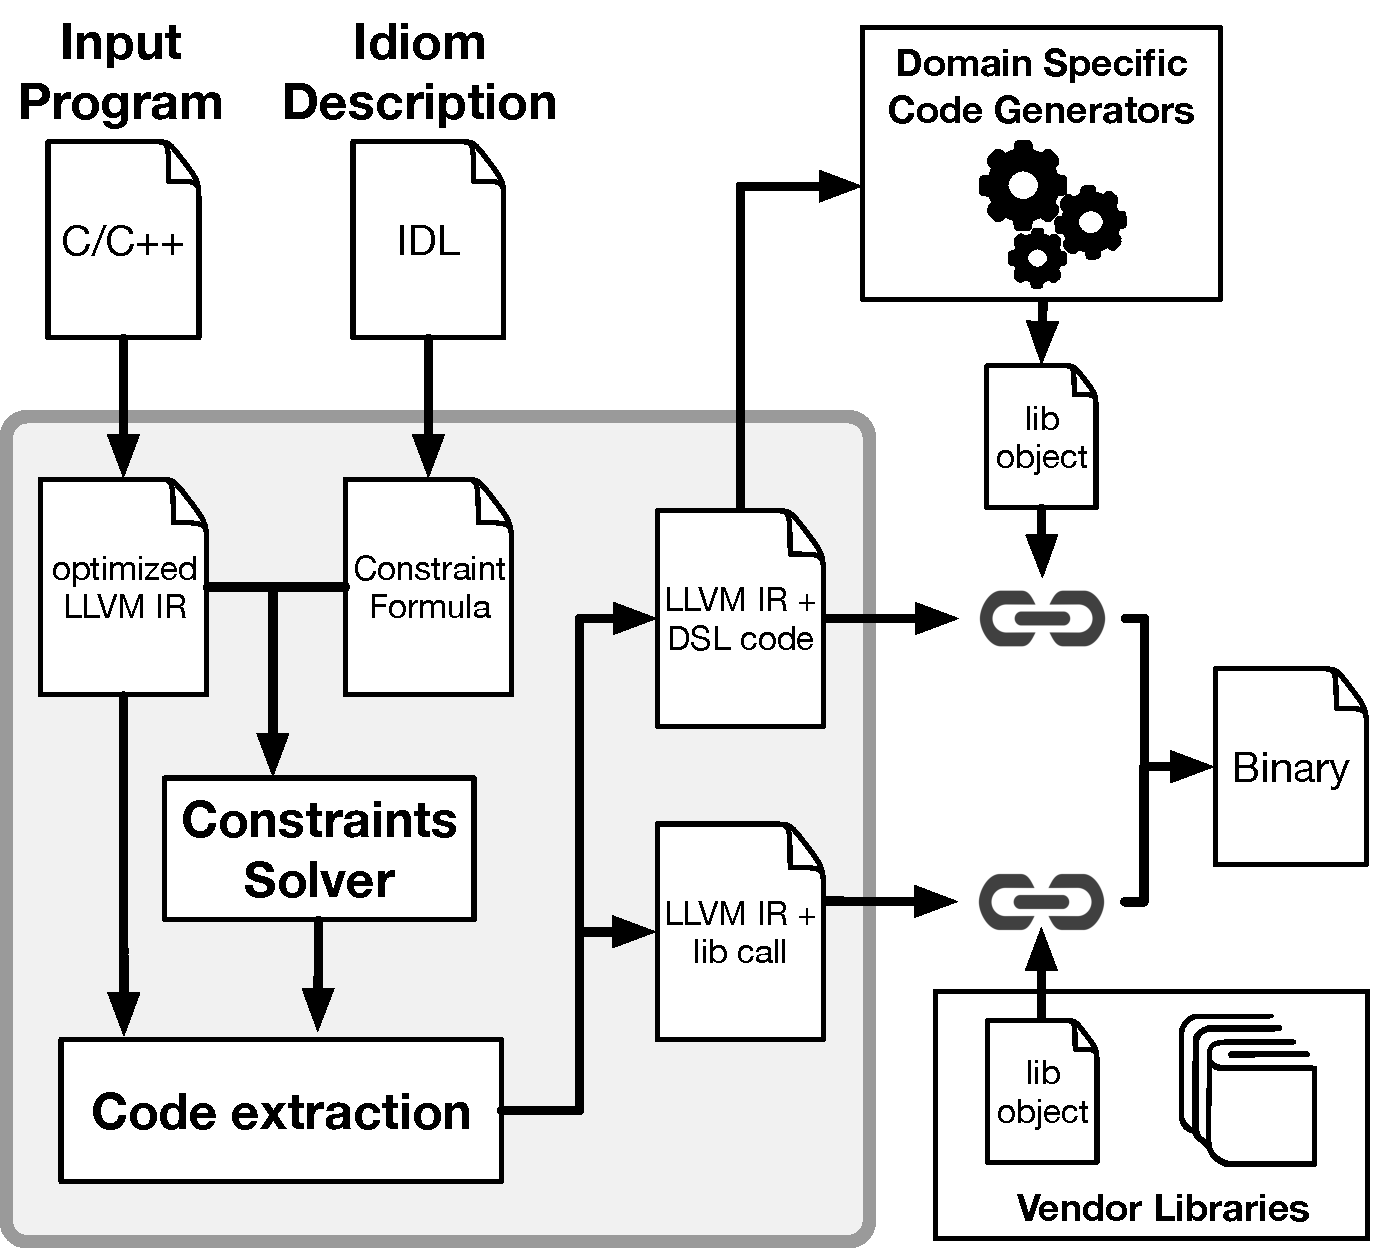
\includegraphics[width=\linewidth]{figures/compiler_flow.pdf}
    \caption{Workflow of the IDL acceleration system:
             The IDL solver recognises idiomatic loops in the optimised LLVM IR
             of user programs.
             These loops are extracted and replaced with shim function calls.
             Domain-specific code generators implement these calls as library
             objects, or they are taken directly from pre-generated vendor
             libraries (for idioms without kernel functions).}
    \label{fig:methodology}
\end{figure}

    The source code of the user program at the top left is compiled into
    optimised LLVM IR code.
    The idiom description is parsed and represented internally as a C++
    object, as previously described in \Cref{chapter:theory},
    \Cref{subsec:impl}.
    The solver takes the optimised LLVM IR code and the internal C++
    representation of the constraint formula as inputs.
    It uses backtracking to recognises all idiomatic parts in the user program.

    The recognised idioms and the LLVM IR code are then passed on to the
    transformation phase of the system.
    This phase extracts the idiomatic code sections from the user program and
    reformulates them for appropriate heterogeneous backends.
    For libraries, this means replacing the code covered by the idiom with a
    library call. 

    For DSL interfaces, the process is a little more involved.
    The user code captured by idioms is extracted and replaced with functions
    calls to shim interfaces.
    The extracted code features are translated into the appropriate DSL.
    External DSL compilers are responsible for optimising this DSL code and
    generating library objects that implement the required function interfaces.
    The translation to DSL mainly involves representing the kernel functions.
    Idioms without kernel functions correspond to fixed DSL programs and
    require no additional work.
    The generated code is linked with the object code from the user program.

    Determining the best heterogeneous API to target for a given platform, and
    the best of several overlapping idioms to exploit, will become an essential
    consideration as the number of idioms and APIs grows.
    For the results in this chapter, all applicable libraries and DSLs were
    evaluated, and the best-performing versions selected after profiling.

\subsection{Accelerating Sparse Linear Algebra}

    Sparse linear algebra is central to many scientific codes and increasingly
    important as a basis for graph algorithms and data analytics
    \cite{Kepner2015GraphsMA}, but it contains indirect data accesses that
    limit compiler optimisation.
    Instead of relying on tooling support, programmers use numerical libraries
    that are hand-optimised and target accelerator hardware.
    This reliance on libraries comes at a cost, however, as it ties programs
    into vendor-specific software ecosystems and results in non-portable code.
    The IDL approach offers an alternative by recognising sparse linear algebra
    kernels in compiler intermediate representation and incorporating the
    domain-specific backends without source code changes.

    The code at the top of \Cref{fig:spmvexample1} is the performance
    bottleneck of the ``Conjugate Gradient'' program from the NAS
    Parallel Benchmarks, with the corresponding LLVM~IR code shown underneath.
    This bottleneck loop implements a standard operation from sparse linear
    algebra, namely the multiplication of a sparse matrix in
    Compressed Sparse Row (CSR) format with a dense vector.
    This computation is supported on accelerator hardware, using well-optimised
    libraries such as cuSPARSE and clSPARSE.
    However, compilers are unable to recognise and accelerate the computation
    automatically.

    The structure of this sparse linear algebra computation has several features
    that make it unsuitable for most established compiler optimisations.
    Firstly, the iteration domain of the nested loop is memory-dependent
    (line 3).
    Secondly, there is indirect memory access (line~4).
    This makes the iteration domain of the loop nest non-polyhedral
    and the access structure to memory non-affine.
    Under these conditions, not only do simple data dependence models fail,
    but so do sophisticated analyses based on the polyhedral model.

    IDL can express this sparse idiom, as derived in \Cref{sec:idioms},
    \Cref{csr_lilacwhat_fig}.
    The ``Conjugate Gradient'' LLVM IR code, together with the
    ``{\tt SPMV\_CSR}'' IDL specification, are input to the constraint solver,
    which outputs a constraint solution, as shown in \Cref{fig:spmvexample2}.
    In the solution, different values from the LLVM IR have been assigned to all
    IDL variables in the ``{\tt SPMV\_CSR}'' specification.

    \Cref{fig:spmvexample3} shows how this solution is used to generate a
    call to a cuSPARSE procedure.
    The individual solution variables are inserted into the
    ``{\tt cusparseDcsrmv}'' code template as function arguments. 
    The original code is then cut out and replaced with this function call.
    In practice, this involved a shim function that manages the device context
    and memory transfers from and to the GPU.
    Finally, the cuSPARSE library was linked with the object code produced by
    the Clang compiler, resulting in a speedup of $17\times$ on a GPU as
    described in more detail in \Cref{sec:idiomresults}.

    Central to this approach is the ability to detect computational idioms
    reliably.
    The next section derives in detail the formulation of sparse and dense
    linear algebra, as well as stencils, in the Idiom Detection Language.

\begin{figure}[p]
    \begin{lstlisting}[language=MyCpp, basicstyle=\linespread{0.75}\small\ttfamily]
for (j = 0; j < ([{\bf m}]); j++) {
  d = 0.0;
  for (k = ([{\bf rowstr }])[j]; k < ([{\bf rowstr}])[j+1]; k++)
    d = d + ([{\bf a}])[k]*([{\bf z}])[([{\bf colidx}])[k]];
  ([{\bf r}])[j] = d; }
\end{lstlisting}
\vspace{-4.4mm}
\begin{lstlisting}[language={LLVM}, basicstyle=\linespread{0.75}\tiny\ttfamily,
                   label={fig:spmvexample1}, caption={Sparse linear algebra in C and LLVM IR}]
; <label>:2:
  %j = phi i64 [ %j_next, %12 ], [ 0, %1 ]
  %j_cond = icmp slt i64 %j, ([{\bf \%m}])
  br i1 %j_cond, label %3, label %13([\vspace{1mm}])
; <label>:3:
%4 = getelementptr i32, i32* ([{\bf \%rowstr}]), i64 %j
  %5 = load i32, i32* %4
  %j_next = add nuw nsw i64 %j, 1
  %6 = getelementptr i32, i32* ([{\bf \%rowstr}]), i64 %j_next
  %7 = load i32, i32* %6
  %k_begin = sext i32 %5 to i64
  %k_end = sext i32 %7 to i64
  br label %8([\vspace{1mm}])
; <label>:8:
  %k = phi i64 [ %k_next, %9 ], [ %k_begin, %dnext ]
  %d = phi double [ 0.0, %3 ], [ %d_next, %9 ]
  %k_cond = icmp slt i64 %iv, %k_end
  br i1 %k_cond, label %9, label %12([\vspace{1mm}])
; <label>:9:
  %a_addr = getelementptr double, double* ([{\bf \%a}]), i64 %k
  %a_load = load double, double* %a_addr
  %cix_addr = getelementptr i32, i32* ([{\bf \%colidx}]), i64 %k
  %cix_load = load i32, i32* %cix_addr
  %10 = sext i32 %cix_load to i64
  %z_addr = getelementptr double, double* ([{\bf \%z}]), i64 %10
  %z_load = load double, double* %z_addr
  %11 = fmul double %a_load, %z_load
  %d_next = fadd double %d, %11
  %k_next = add nsw i64 %k, 1
  br label %8([\vspace{1mm}])
; <label>:12:
  %r_addr = getelementptr double, double* ([{\bf \%r}]), i64 %j
  store double %d, double* %r_addr
  br label %2
\end{lstlisting}
\vspace{-0.287cm}
%\end{figure}

\centering
\vspace{0.0em}
{\centering
\begin{minipage}{0.05\linewidth}
\vspace{0pt}
\centering
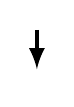
\begin{tikzpicture}[ultra thick]
 \draw [black,   -latex      ] (0,0.5) -- (0,0) node [] {};
\end{tikzpicture}
\end{minipage}
\begin{minipage}{\linewidth}
% \vspace{-5pt}
\centering
\textbf{Idiom detection with IDL program in \Cref{fig:spmv}}
\end{minipage}
\begin{minipage}{0.05\linewidth}
\vspace{0pt}
\centering
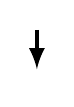
\begin{tikzpicture}[ultra thick]
 \draw [black,   -latex      ] (0,0.5) -- (0,0) node [] {};
\end{tikzpicture}
\end{minipage}
}

%\begin{figure}
{\centering
\footnotesize 
\begin{tabular}{l|l}
\textbf{Variable Name} & \textbf{Assigned IR Value}\\
\hline
iterator                    & \texttt{\%j}\\
inner.iter\_begin           & \texttt{\%k\_begin}\\
inner.iter\_end             & \texttt{\%k\_end}\\
inner.iterator              & \texttt{\%k}\\
idx\_read.value             & \texttt{\%cix\_load}\\
indir\_read.value           & \texttt{\%a\_load}\\
seq\_read.value             & \texttt{\%z}\\
\end{tabular}
\hspace{0.5cm}
\begin{tabular}{l|l}
\textbf{Variable Name} & \textbf{Assigned IR Value}\\
\hline
output.address              & \texttt{\%r\_addr}\\
iter\_begin                 & \texttt{0}\\
iter\_end                   & \texttt{\%\bf m}\\
idx\_read.base\_pointer     & \texttt{\%\bf colidx}\\
seq\_read.base\_pointer     & \texttt{\%\bf a}\\
indir\_read.base\_pointer   & \texttt{\%\bf z}\\
\dots                       & \dots\vspace{-0.5mm}\\
\end{tabular}

}

\caption{Constraint solution for sparse mv}
\label{fig:spmvexample2}
%\end{figure}

\centering
\vspace{0.0em}
{\centering
\begin{minipage}{0.05\linewidth}
\vspace{0pt}
\centering
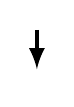
\begin{tikzpicture}[ultra thick]
 \draw [black,   -latex      ] (0,0.5) -- (0,0) node [] {};
\end{tikzpicture}
\end{minipage}
\begin{minipage}{\linewidth}
% \vspace{-5pt}
\centering
\textbf{Code generation: insert arguments, replace code}
\end{minipage}
\begin{minipage}{0.05\linewidth}
\vspace{0pt}
\centering
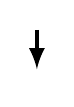
\begin{tikzpicture}[ultra thick]
 \draw [black,   -latex      ] (0,0.5) -- (0,0) node [] {};
\end{tikzpicture}
\end{minipage}
}


%\begin{figure}
\begin{lstlisting}[language=C, basicstyle=\linespread{0.75}\small\ttfamily,
                   label={fig:spmvexample3}, caption={Generated function call to cuSPARSE}]
cusparseDcsrmv(context,
    CUSPARSE_OPERATION_NON_TRANSPOSE, ([{\bf m}]), n,
    ([{\bf rowstr}])[([{\bf m}])+1]-([{\bf rowstr}])[0], &gpu_1, descr, gpu_([{\bf a}]),
    gpu_([{\bf rowstr}]), gpu_([{\bf colidx}]), gpu_([{\bf z}]), &gpu_0, gpu_([{\bf r}]));
\end{lstlisting}
\vspace{-0.287cm}
\end{figure}

\section{Specification of Idioms in IDL}
\label{sec:idioms}

    The specification of computational idioms in IDL requires careful
    handling of the arising complexity, using the modularity features that
    the language provides.
    Control flow constructs, memory access patterns, and additional data flow
    constraints are defined independently and then combined to form the complete
    specifications.
    This section extends upon the previously defined building blocks from
    \Cref{chapter:candl,chapter:reductions}.

\subsection{Sparse Linear Algebra}

    The most frequently used performance-critical sparse linear algebra routines
    are variations on the multiplication of a sparse matrix with a dense vector
    (SPMV).
    Capturing the many different memory access patterns is crucial for these
    sparse linear algebra routines.
    On the other hand, the control flow is very rigid.

    \Cref{spmvbase} shows the basic skeleton of the SPMV idiom:
    there are two for-loops, the ``{\tt outer\_loop}'' and the
    ``{\tt inner\_loop}''.
    Naturally, ``{\tt outer\_loop}'' contains ``{\tt inner\_loop}''
    (lines 4--7).
    The outer loop is a standard for-loop (line 2), while the inner loop is a
    for-loop contains a generalised dot product (line 3).
    Specifically, the ``{\tt DotProductFor}'' specification requires that the
    loop contains a scalar reduction variable that is incremented by the result
    of a floating-point multiplication of two values ``{\tt src1}'' and
    ``{\tt src2}'' in every iteration.
    This skeleton is completed depending on the sparse matrix format, defining
    the specific computations and data flow that yields ``{\tt src1}'' and
    ``{\tt src2}''.

\begin{figure}[p]
\lstset {
 basicstyle=\linespread{1.069}\small\ttfamily
}
\begin{lstlisting}[language=IDL, label={spmvbase}, caption=
   {Skeleton of the sparse matrix-vector product (SPMV) constraint
    specification in IDL: The precise sparse access patterns are specific to
    chosen storage formats for sparse matrices.}]
Constraint SPMV
( inherits For at {outer_loop} and
  inherits DotProductFor at {inner_loop} and
  {outer_loop.begin} strictly
      control flow dominates {inner_loop.begin} and
  {outer_loop.end} strictly
      control flow post dominates {inner_loop.end} and
([\dots])
\end{lstlisting}
\end{figure}

\begin{figure}[p]
\hfill
\begin{minipage}[b]{0.3\linewidth}
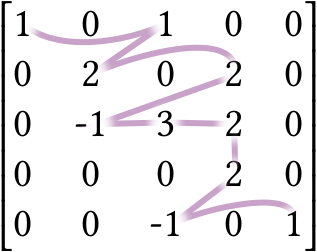
\includegraphics[width=0.95\linewidth]{figures/csrorder.png}
\end{minipage}
\hfill
\begin{minipage}[b]{0.5\linewidth}
\begin{align*}
\text{\bf val} =& \begin{bmatrix}
1\ \ 1\ \ 2\ \ 2\ \ \text{-}1\ \ 3\ \ 2\ \ 2\ \ \text{-}1\ \ 1\\
\end{bmatrix}\\[4mm]
\text{\bf col\_ind} =& \begin{bmatrix}
0\ \ 2\ \ 1\ \ 3\ \ 1\ \ 2\ \ 3\ \ 3\ \ 2\ \ 4\\
\end{bmatrix}\\[4mm]
\text{\bf row\_ptr} =& \begin{bmatrix}
0\ \ 2\ \ 4\ \ 7\ \ 8\ \ 10\\
\end{bmatrix}
\end{align*}
\end{minipage}
\hfill

\vspace{0.8em}
\hrule
\vspace{0.3em}

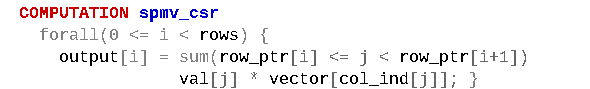
\includegraphics[width=\linewidth]{figures/spmvcsrwhat.pdf}
\vspace{-1.5em}
\lstset {
 basicstyle=\linespread{1.069}\small\ttfamily
}
\begin{lstlisting}[language=IDL,firstnumber=7]
([\dots])([\ttfamily\small\color{color_comment}{\hspace{1.6mm}\# Set top-level expression:~output[<1>] = <2> * <3>~~~~~~~~~~~stack=(1,2,3)}])
  inherits VectorStore([\tt\color{color_comment}{~\#~1:~output[i]~~~~~~~~~~~~~~~~~~~~~~~~stack=(2,3)}])
      with {outer_loop}          as {scope}
       and {outer_loop.iterator} as {input_index} at {output} and
  inherits VectorRead ([\tt\color{color_comment}{~\#~2:~val[j]~~~~~~~~~~~~~~~~~~~~~~~~~~~stack=(3)}])
      with {outer_loop}          as {scope}
       and {inner_loop.src1}     as {value}([{\tt\color{color_comment}\#<-case <2>])
       and {inner_loop.iterator} as {input_index} at {val} and
  inherits VectorRead ([\tt\color{color_comment}{~\#~3:~vector[col\_ind[<4>]]~~~~~~~~~~~~~stack=(4)}])
      with {outer_loop}      as {scope}
       and {inner_loop.src2} as {value}([{\tt\color{color_comment}\#<-case <3>])
       and {col_ind.value}   as {input_index} at {vector} and
  inherits VectorRead ([\tt\color{color_comment}{~\#~4:~col\_ind[j]~~~~~~~~~~~~~~~~~~~~~~~stack=()}])
      with {outer_loop}          as {scope}
       and {inner_loop.iterator} as {input_index} at {col_ind} and
  inherits ReadForLoopRanges
     with {outer_loop}          as {scope}
      and {inner_loop}          as {for}
      and {outer_loop.iterator} as {input_index} at {row_ptr})
End
\end{lstlisting}
\caption{Compressed Sparse Row in IDL:
         The top section of the figure shows the different arrays involved.
         The pseudocode in the middle of the figure informs the completion of
        \Cref{spmvbase} at the bottom.
         Walking through the expressions and emitting IDL code one-by-one is
         sufficient.}
\label{csr_lilacwhat_fig}
\end{figure}

\subsubsection{Compressed Sparse Row}

    The Compressed Sparse Row (CSR) format is one of the most widely used
    formats for sparse matrices \cite{doi:10.1137/1.9780898718003}.
    An example matrix stored in CSR format is shown at the top of
    \autoref{csr_lilacwhat_fig}.
    The 5$\times$5 matrix at the top left is stored in the three separate arrays
    at the top right: ``\textbf{val}'', ``\textbf{col\_ind}'', and
    ``\textbf{row\_ptr}''.

    All non-zero entries of the matrix are stored in a flat array
    ``\textbf{val}'' in a row-by-row order.
    The ``\textbf{col\_ind}'' array stores the column position for each value.
    Finally, the ``\textbf{row\_ptr}'' array stores the beginning of each row of
    the matrix as an offset into the other two arrays.
    The number of rows in the matrix is given directly by the length of the
    ``\textbf{row\_ptr}'' array minus one.
    However, the number of columns is not explicitly stored.

    The middle row of \autoref{csr_lilacwhat_fig} shows the corresponding
    SPMV computation in pseudocode.
    Finally, the bottom of the figure shows the continuation of the
    ``{\tt SPMV}'' specification for CSR matrices in IDL.
    This continuation is immediately derived by walking through the pseudocode
    expressions and emitting ``{\tt inherits}'' directives to the corresponding
    IDL subprograms.

\subsubsection{Jagged Diagonal Storage}

    For Jagged Diagonal Storage (JDS) \cite{doi:10.1137/0910073}, the rows of
    the matrix are permuted such that the number of nonzeros per row  decreases.
    The permutation is stored in a vector ``\textbf{perm}'', the number of
    nonzeros per row in ``\textbf{nzcnt}''.
    The nonzero entries are then stored in an array ``\textbf{val}'' in the
    following order: the first nonzero entry in each row, then the second
    nonzero entry in each row and so on.
    The array ``\textbf{col\_ind}'' stores the column for each of the values and
    ``\textbf{jd\_ptr}'' stores offsets into ``\textbf{val}'' and
    ``\textbf{col\_idx}''.

    \autoref{jds_lilacwhat_fig} demonstrates this format on the example sparse
    matrix from \autoref{csr_lilacwhat_fig}, and derives the corresponding IDL
    code for the ``{\tt SPMV\_JDS}'' idiom underneath.
    Note that the sparse matrix in this example is shown after the permutation
    operation that JDS requires.

\begin{figure}[p]
\hfill
\begin{minipage}[b]{0.3\linewidth}
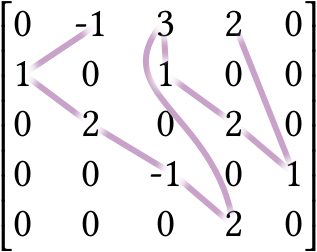
\includegraphics[width=0.9\linewidth]{figures/jdsorder.png}
\end{minipage}
\hfill
\begin{minipage}[b]{0.65\linewidth}
\footnotesize
\begin{align*}
\text{\bf perm} =& \begin{bmatrix}1\ \ 2\ \ 0\ \ 4\ \ 3\\\end{bmatrix}\\[-0.75mm]
\text{\bf val} =& \begin{bmatrix}\text{-}1\ \ 1\ \ 2\ \ \text{-}1\ \ 2\ \ 3\ \ 1\ \ 2\ \ 1\ \ 2\\\end{bmatrix}\\[-0.75mm]
\text{\bf col\_ind} =& \begin{bmatrix}1\ \ 0\ \ 1\ \ 2\ \ 3\ \ 2\ \ 2\ \ 3\ \ 4\ \ 3\\\end{bmatrix}\\[-0.75mm]
\text{\bf jd\_ptr} =& \begin{bmatrix}0\ \ 5\ \ 9\ \ 10\\\end{bmatrix}\\[-0.75mm]
\text{\bf nzcnt} =& \begin{bmatrix}3\ \ 2\ \ 2\ \ 2\ \ 1\end{bmatrix}
\end{align*}
\end{minipage}
\hfill

\vspace{0.8em}
\hrule
\vspace{0.3em}

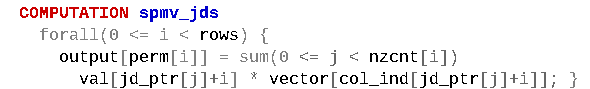
\includegraphics[width=\linewidth]{figures/spmvjdswhat.pdf}
\vspace{-1.5em}
\lstset {
 basicstyle=\linespread{1.271}\small\ttfamily
}
\begin{lstlisting}[language=IDL,firstnumber=7]
([\dots])([{\ttfamily\small\color{color_comment}\hspace{1.6mm}\#~Set top-level expression:~output[<1>]~=~<2>~*~<3>~~~~~~~~~~stack=(1,2,3)}])
  inherits VectorStore([{\tt\color{color_comment}~\#~1:~output[perm[<4>]]~~~~~~~~~~~~~~~~stack=(4,2,3)}])
      with {outer_loop} as {scope}
       and {perm.value} as {input_index} at {output} and
  inherits VectorRead ([{\tt\color{color_comment}~\#~4:~perm[i]~~~~~~~~~~~~~~~~~~~~~~~~~~stack=(2,3)}])
      with {outer_loop}          as {scope}
       and {outer_loop.iterator} as {input_index} at {perm} and
  inherits VectorRead ([{\tt\color{color_comment}~\#~2:~val[(tmp1)=<5>]~~~~~~~~~~~~~~~~~~stack=(5,3)}])
      with {outer_loop}      as {scope}
       and {inner_loop.src1} as {value}([{\tt\color{color_comment}\#<-case <2>])
       and {tmp1.value}      as {input_index} at {val} and
  inherits Addition   ([{\tt\color{color_comment}~\# 5:~(tmp1)=jd\_ptr[<6>]+i~~~~~~~~~~~~~stack=(6,3)}])
      with {jd_ptr.value}        as {input}
       and {outer_loop.iterator} as {addend} at {tmp1} and
  inherits VectorRead ([{\tt\color{color_comment}~\#~6:~jd\_ptr[i]~~~~~~~~~~~~~~~~~~~~~~~~stack=(3)}])
      with {outer_loop}          as {scope}
       and {inner_loop.iterator} as {input_index} at {jd_ptr} and
  inherits VectorRead ([{\tt\color{color_comment}~\#~3:~vector[<7>]~~~~~~~~~~~~~~~~~~~~~~stack=(7)}])
      with {outer_loop}      as {scope}
       and {inner_loop.src2} as {value}([{\tt\color{color_comment}\#<-case <3>])
       and {col_ind.value}   as {input_index} at {vector} and
  inherits VectorRead ([{\tt\color{color_comment}~\#~7:~col\_ind[(tmp1)=<5>]~~~~~~~~~~~~~~stack=()}])
      with {outer_loop} as {scope}
       and {tmp1.value} as {input_index} at {col_ind} and
  inherits ReadForLoopIterations
     with {outer_loop}          as {scope}
      and {inner_loop}          as {for}
      and {outer_loop.iterator} as {input_index} at {read_range}
\end{lstlisting}
\caption{Jagged Diagonal Storage in IDL:
         The top section of the figure shows the different arrays involved.
         The pseudocode in the middle of the figure informs the completion of
         \Cref{spmvbase} at the bottom.
         Walking through the expressions and emitting IDL code one-by-one is
         sufficient.}
\label{jds_lilacwhat_fig}
\end{figure}

\subsection{Dense Linear Algebra}

    Describing dense linear algebra does not require storage format
    consideration aside from the simple {\it row-major} and {\it column-major}
    distinction.
    The generalised matrix multiplication idiom is shown in \Cref{fig:gemm}.
    The control flow is captured by three nested for-loops.
    Inside these loops, the memory access is characterised by three matrix
    accesses, each with a different subset of the loop iterators.
    The corresponding ``{\tt MatrixRead}'' and ``{\tt MatrixWrite}'' idioms
    model generic access to matrices, allowing strides and transpositions.
    The floating-point calculations in the inner loop are encapsulated by
    the ``{\tt DotProductForAlphaBeta}'' idiom.
    This extends the ``{\tt DotProductFor}'' specification with the linear
    combination that is part of the generalised matrix multiplication idiom
    ($C\gets\alpha AB+\beta C$).

\begin{figure}[H]
\lstset {
 basicstyle = \linespread{0.865}\ttfamily
}
\begin{lstlisting}[language=IDL, label={fig:gemm}, caption=
   {IDL specification of the generalised dense matrix-vector multiplication
    (GEMM)\leftskip=0pt\rightskip=0pt}]
Constraint GEMM
( inherits ForNest(N=3) and
  inherits MatrixStore
      with {iterator[0]} as {col}
       and {iterator[1]} as {row}
       and {begin} as {begin} at {output} and
  inherits MatrixRead
      with {iterator[0]} as {col}
       and {iterator[2]} as {row}
       and {begin} as {begin} at {input1} and
  inherits MatrixRead
      with {iterator[1]} as {col}
       and {iterator[2]} as {row}
       and {begin} as {begin} at {input2} and
  inherits DotProductForAlphaBeta
      with {loop[2]}        as {loop}
       and {input1.value}   as {src1}
       and {input2.value}   as {src2}
       and {output.address} as {update_address})
End
\end{lstlisting}
\end{figure}

\subsection{Stencils}

    \Cref{fig:stencilcompute} shows the base version of the stencil idiom.
    Stencils consist of a loop nest with multi-dimensional memory access
    (lines 3--5) to store the updated cell value.
    The updated value is computed by a kernel function (lines 12--13) using
    several values that are constrained by ``{\tt StencilRead}'' (lines 6--10),
    which specifies multi-dimensional array access with only constant offsets in
    all dimensions.

\begin{figure}[t]
\begin{lstlisting}[language=IDL, label={fig:stencilcompute}, caption=
   {IDL specification of a basic stencil computation}]
Constraint Stencil
( inherits ForNest and
  inherits PermMultidStore
      with {iterator} as {input}
       and {begin}    as {begin} at {write} and
  collect i 32
  ( inherits StencilRead
        with {write.input_index} as {input}
         and {kernel.inputs[i]}  as {value}
         and {begin} as {begin}  at {reads[i]}) and
  {kernel.output} is first argument of {write.store} and
  inherits KernelFunction
      with {loop[0]} as {scope} at {kernel})
End
\end{lstlisting}
\end{figure}

\section{Comparison to Syntactic Matching}
\label{sec:syntacticmatching}

    The idiom descriptions may at first appear to be shallow syntactic pattern
    matching, but the approach is intrinsically more powerful.
    Because it operates on the IR level, the solver can detect idioms that are
    written in a superficially distinct style but are semantically equivalent.

    For example, \Cref{fig:gemmexamples} shows two syntactically distinct
    programs, which nevertheless are both implementations of general matrix
    multiplication.
    The solver -- using \Cref{fig:gemm} -- discovers that both of these
    loop nests are instances of GEMM and can be replaced with the same API call.

    The reverse is also true: the solver distinguishes syntactically identical
    but semantically distinct programs.
    \Cref{fig:gemmcounterexamples} shows such an example.
    The loop nest in lines 7--11 appears to compute a standard GEMM, but in fact,
    the matrices are not stored contiguously, and acceleration with standard
    libraries is impossible.

\begin{figure}[p]
\lstset{
 basicstyle = \linespread{1.168}\ttfamily
}
\begin{lstlisting}[language=MyCpp]
for (int mm = 0; mm < m; ++mm) {
  for (int nn = 0; nn < n; ++nn) {
    float c = 0.0f;
    for (int i = 0; i < k; ++i) {
      float a = A[mm + i * lda]; 
      float b = B[nn + i * ldb];
      c += a * b;
    }
    C[mm+nn*ldc] =
        C[mm+nn*ldc] * beta + alpha * c;
  }
}
\end{lstlisting}
\begin{lstlisting}[language=MyCpp,label={fig:gemmexamples},caption=
   {Two matching instances of ``{\tt GEMM}'':
    Although both loop nests are implemented very differently, they both match
    the same IDL specification and can be accelerated identically.}]
double M1[1000][1000];
double M2[1000][1000];
double M2[1000][1000];

//...

for(int i = 0; i < 1000; i++)
    for(int j = 0; j < 1000; j++) {
        M3[i][j] = 0.0f;
        for(int k = 0; k < 1000; k++)
           M3[i][j]+=M1[i][k]*M2[k][j]; }
\end{lstlisting}
\begin{lstlisting}[language=MyCpp,label={fig:gemmcounterexamples},caption=
   {This C program that does not match ``{\tt GEMM}''.
    Although the loop syntax is identical to the matching example from
    \Cref{fig:gemmexamples}, the different types of the matrices prevent
    detection.
    This is desirable:
    Established backends are incompatible with such non-contiguous memory
    layout.}]
double *M1[1000];
double *M2[1000];
double *M2[1000];

//...

for(int i = 0; i < 1000; i++)
    for(int j = 0; j < 1000; j++) {
        M3[i][j] = 0.0f;
        for(int k = 0; k < 1000; k++)
           M3[i][j]+=M1[i][k]*M2[k][j]; }
\end{lstlisting}
\end{figure}

    There are limitations to this semantic matching.
    In particular, the use of low-level manual optimisations that circumvent the
    usual intermediate representation, e.g.\ SIMD intrinsics, may distort the
    algorithms beyond recognition.
    In practice, this is rarely encountered.

\section{Targeting Heterogeneous Backends}

    After idiom detection, user programs must be transformed to exploit the
    relevant APIs.
    Two types of heterogeneous APIs were targeted:
    libraries and domain-specific languages with their optimising compilers.

\subsection{Domain-Specific Libraries}

    Libraries provide narrow interfaces but are often highly optimised.
    For example, the cuBLAS library is only suitable for a limited set of dense
    linear algebra operations and only works on Nvidia GPUs, but its
    implementation provides outstanding performance.
    For sparse linear algebra, the vendor-provided cuSPARSE, clSPARSE, and
    Intel MKL libraries were used.
    For dense BLAS routines, the available backends were cuBLAS, clBLAS,
    CLBlast, and MKL.

\subsection{Domain-Specific Code Generators}

    Domain-Specific Languages provide wider interfaces than libraries and allow
    problems to be expressed as compositions of dedicated language constructs.
    Most importantly, this allows DSLs to capture kernel functions of idioms
    that are higher-order functions, e.g.\ stencils and reductions.
    The domain-specific optimising compiler then specialises the program for the
    target hardware.

    The end result is a library object, which can then be treated
    identically to pre-generated vendor libraries.
    For this research,  domain-specific code generators are, therefore,
    effectively used as on-demand library generators.
    The evaluation used Halide and Lift as domain-specific code generators.

    \paragraph*{Halide}~\citet{Ragan-Kelley2013Halide} introduced a language and
    optimising compiler targeted at image processing applications.
    Optimised code is generated for CPUs as well as GPUs.
    Halide separates the functional description of the problem from the
    description of the implementation.
    This involves a separate execution \emph{schedule}.
    This separation allows retargeting of Halide programs to different platforms
    without touching the core program.
    Some of the stencil and linear algebra idioms were translated into Halide.
    However, stencils involving control flow in their kernel were not
    expressible in Halide and excluded for this backend.

    \paragraph*{Lift}~\citet{steuwer15rewrite} introduced an optimising code
    generator based on rewrite rules \citep{SteuwerRD17, HagedornSSGD18}.
    The Lift language consists of functional parallel patterns such as
    ``{\tt map}'' and ``{\tt reduce}'' that  express a range of parallel
    applications.
    Stencil idioms, complex reductions and linear algebra idioms were translated
    to Lift.

\section{Translating Computational Idioms}

    This section describes how the detected idioms are mapped to the previously
    described library APIs and domain-specific languages.
    The two types of APIs (library interfaces and domain-specific languages) are
    treated individually.

\subsection{Domain-Specific Libraries}

    For library call interfaces, the original code is removed, and an
    appropriate function call is inserted.
    The solution that is generated by the solver using the IDL program contains
    both the IR instructions to remove as well as the arguments that are to be
    used for the function call.

    For example, in the case of the {\tt GEMM} program that was shown in
    \Cref{fig:gemm}, the original code is removed by deleting the IR
    instruction at {\tt output.store\_instr} explicitly, which captures the
    store instruction of the {\tt MatrixStore} subprogram.
    The remaining cleanup is left to the standard {\em dead code elimination}
    pass.
    The arguments that specify the matrix dimensions are taken from
    {\tt ForNest} in combination with the stride and offset determined by
    {\tt MatrixRead} and {\tt MatrixWrite}.

    The mapping of solution variables to the arguments of the generated function
    call needs to be implemented individually for each backend, as it cannot be
    described using IDL itself.
    Once the code is replaced, LLVM continues with code generation as usual.

\subsection{Domain-Specific Code Generators}

    For domain-specific code generators, the situation is a bit more involved
    than for libraries.
    Stencils and Complex Reduction and Histogram Computations are higher-order
    functions, containing kernel functions or reduction operators that have to
    be represented for the DSL.

    For each combination of idiom and DSL, there is a parameterised
    skeleton program.
    This skeleton is then specialised for the appropriate data types and numeric
    parameters as well as the kernel function or reduction operator.

    Numerical parameters are picked from the constraint solution in the same way
    as previously described for library call interfaces.
    Also, from the constraint solution, the loop body that contains the kernel
    function or reduction operator is accessible, as well as the input values
    and the result value used.
    This information is enough to cut out the kernel function, which is then
    used to generate code appropriate for the DSL backends.

    \paragraph*{Halide}
    is a language embedded in C++.
    It requires a syntax tree of the kernel functions that built using a class
    hierarchy.
    However, Halide does not support control flow in the kernel functions,
    making code generation easier than for Lift in practice.
    The relevant kernel functions contain only a few LLVM IR instructions, which
    are easily assembled into Halide expressions.

    \paragraph*{Lift}
    expects stencil kernels or reduction operators to be sequential C code with
    a specific function interface, which it requires for generating valid
    OpenCL code.
    As the kernel functions are only directly available as LLVM IR code from the
    constraint solution, the implementation of a rudimentary LLVM IR to C
    backend was necessary to generate input for the Lift compiler.

\begin{figure}[H]
\begin{lstlisting}[language=LIFT,escapechar=|,
                   label={fig:liftmxm},caption=
   {GEMM in Lift is expressed with the higher-order functions
    ``{\tt zip}'', ``{\tt map}'', ``{\tt reduce}''.\leftskip=0pt\rightskip=0pt}]
float mult(float x, float y) { return x*y; }
float add(float x, float y) { return x+y; }

gemm_in_lift(A, B, C, alpha, beta) {
 map(fun(a_row, c_row) {
  map(fun(b_col, c) {
   map(fun(ab){ add(mult(alpha, ab), mult(beta, c))},
    |\label{line:dot}|reduce(add, 0.0f, map(mult, zip(a_row, b_col))))
  }, zip(transpose(B), c_row))
 }, zip(A, C))
}
\end{lstlisting}
\end{figure}

    \paragraph*{Example}
    After code for the DSLs was generated, it is passed to the DSL code
    generator.
    \Cref{fig:liftmxm} shows an example of the Lift code generated for GEMM
    ({\tt gemm\_in\_lift}).
    It performs a dot product (expressed in line~\ref{line:dot} using the Lift
    skeletons {\tt zip}, {\tt map}, and {\tt reduce}) for each row of
    matrix A ({\tt a\_row}) and column of matrix B ({\tt b\_col}).
    This code is compiled by Lift into optimised OpenCL code.

\subsection{Aliasing}

    Since idiom detection works statically, pointer aliasing cannot be ruled out
    conclusively, which can make transformations unsound.
    For dense linear algebra, this is easily solved with simple runtime
    checks for non-overlapping memory.
    In case of any detected aliasing, the program falls back to the naive
    implementation.

    However, for sparse linear algebra, this is not as straightforward.
    While aliasing can still be ruled out by dynamic checks, this involves
    additional overhead, as the indices of the indirect array access need to
    be monitored.
    This overhead can be amortised over multiple calls if the indirection array
    remains unchanged, which was the case for the programs involved in the
    evaluation.

    Such techniques to rule out aliasing are important but orthogonal to the
    detection and transformation methods that are the focus of this chapter.
    In practice, aliasing did not cause problems on any of the benchmark
    programs.
    However, detailed feedback was provided in the form of transformation
    reports that give the user control over the program modifications and allow
    the explicit disabling of the approach in uncertain cases.

\begin{table}[H]
\centering
\begin{tabular}{lrl}
\toprule
\multirow{6}{*}{\bf NPB}
 & BT & Block Tridiagonal Solver\\[-3.0mm]
 & CG & Conjugate Gradient\\[-3.0mm]
 & DC & Data Cube Operator\\[-3.0mm]
 & EP & Embarrassingly Parallel Marsaglia Polar Method\\[-3.0mm]
 & FT & Fast Fourier Transform\\[-3.0mm]
 & IS & Small Integer Bucket Sort \\[-3.0mm]
 & LU & Lower-Upper Symmetric Gauss-Seidel Solver\\[-3.0mm]
 & MG & MultiGrid Approximation\\[-3.0mm]
 & SP & Scalar Pentadiagonal Solver\\[-3.0mm]
 & UA & Unstructured Adaptive Mesh\\
\specialrule{\lightrulewidth}{0pt}{0pt}
\multirow{7}{*}{\bf Parboil}
 & bfs          & Breadth-First Search\\[-3.0mm]
 & cutcp        & Distance-Cutoff Coulombic Potential\\[-3.0mm]
 & histo        & Saturating Histogram\\[-3.0mm]
 & lbm          & Lattice-Boltzmann Method Fluid Dynamics\\[-3.0mm]
 & mri-gridding & Magnetic Resonance Imaging - Gridding\\[-3.0mm]
 & mri-q        & Magnetic Resonance Imaging - Q\\[-3.0mm]
 & sad          & Sum of Absolute Differences (part of MPEG encoding)\\[-3.0mm]
 & sgemm        & Dense Matrix-Matrix Multiply\\[-3.0mm]
 & spmv         & Sparse-Matrix Dense-Vector Multiplication\\[-3.0mm]
 & stencil      & Iterative 3D Jacobi Stencil\\[-3.0mm]
 & tpacf        & Two Point Angular Correlation Function\\
\bottomrule
\end{tabular}
\caption{Overview of the 21 programs used for evaluation, grouped into two
         suites}
\end{table}

\section{Experimental Setup}

    \paragraph*{Benchmarks}
    The approach was applied to all of the sequential C/C++ programs of the NAS
    Parallel Benchmarks, in the versions provided by Seoul National University
    (SNU NPB) \citep{seo2011performance}.
    Additionally, the Parboil benchmarks \citep{Stratton2018} were used,
    giving 21 evaluation programs in total. 

    \paragraph*{Platform and Evaluation}
    The evaluation platform used an AMD A10-7850K APU with a Radeon R7
    integrated GPU (driver version 1912.5) and an Nvidia GTX Titan X external
    GPU (driver version 375.66).
    Execution times were measured as the median over ten runs.

    \paragraph*{Alternative detection approaches}
    There were no readily available compilers performing idiom detection to
    compare against.
    Instead, two parallelising compilers were considered.
    The evaluation examined the ability to parallelise idiomatic code, without
    considering whether the idioms were recognised.
    \Cref{section:competition} provided a detailed discussion of both
    competing tools: Polly and ICC.
    Therefore, they are only presented briefly here.
    It should be borne in mind that the competing compilers aim for
    parallelisation, not idiom detection itself.

    Polly is an LLVM-based polyhedral compiler.
    The SCoPs that Polly detected with the options
    {\tt -O3 -mllvm -polly -mllvm -polly-export} were gathered.
    When Polly captured a SCoP containing an idiom, it was counted as an
    idiom detection.
    This gives an optimistic estimate as to what idiom coverage a polyhedral
    based approach can achieve.

    The Intel C++ Compiler (ICC) is a mature industry strength compiler that
    performs auto-parallelisation.
    All loops that were emitted as parallelisable by
    ``{\tt-parallel -qopt-report}'' and that contained idioms were counted as
    idiom detections.

\section{Results}
\label{sec:idiomresults}

    The approach was evaluated in several steps.
    Firstly, the number of detected idioms and their distribution over the
    benchmark programs was established.
    During this analysis, the runtime of the IDL-enabled Clang compiler was
    measured, and the compile time overhead of the solver over standard
    compilation evaluated.
    Next, the runtime coverage of the idioms was determined for each
    benchmark program, to see where exploitation might be beneficial.

    Where runtime coverage was substantial, speedups over the sequential C code
    are reported.
    Detailed results are given for the performance of each targeted backend
    interface.
    Finally, the evaluation includes comparisons to the handwritten OpenMP and
    OpenCL implementations that are provided with the benchmark suites as
    reference implementations, providing a suitable estimate for the upper
    bound of available performance.

\subsection{Idiom Detection}

    \Cref{detection-figure} shows the different idioms detected across
    all the individual benchmark programs.
    IDL detected both scalar and histogram reductions as well as stencils, dense
    matrix operations and sparse matrix-vector multiplication.
    16 of the 21 programs contained computational idioms that IDL was able to
    identify.
    The most frequently occurring idiom was scalar reduction, present in 10
    of the programs.
    Five of the benchmarks contained histograms; three contained stencils;
    two contained SPMV; and only a single program calculated GEMM.

    \Cref{tab:detection} summarises the number of computational idioms found by
    IDL, Polly, and ICC.
    Polly found three scalar reductions and five stencils, and also detected the
    GEMM operation as a generic SCoP.
    This was counted as a detected idiom, although Polly was unable to apply any
    domain-specific knowledge from linear algebra.
    ICC only recognised scalar reduction, but was much more successful at it
    than Polly, detecting a total of 28 instances.

    Other approaches than IDL did not detect any histogram loops or sparse
    matrix operations.
    In total, IDL detected 60 idioms overall with the increase in compilation
    time shown in figure \Cref{tab:compiletimecost}.
    On average, the compilation time was increased by 82\%. 
    The overhead could be reduced further by optimising the solver.

\begin{figure}[p]
  \centering
  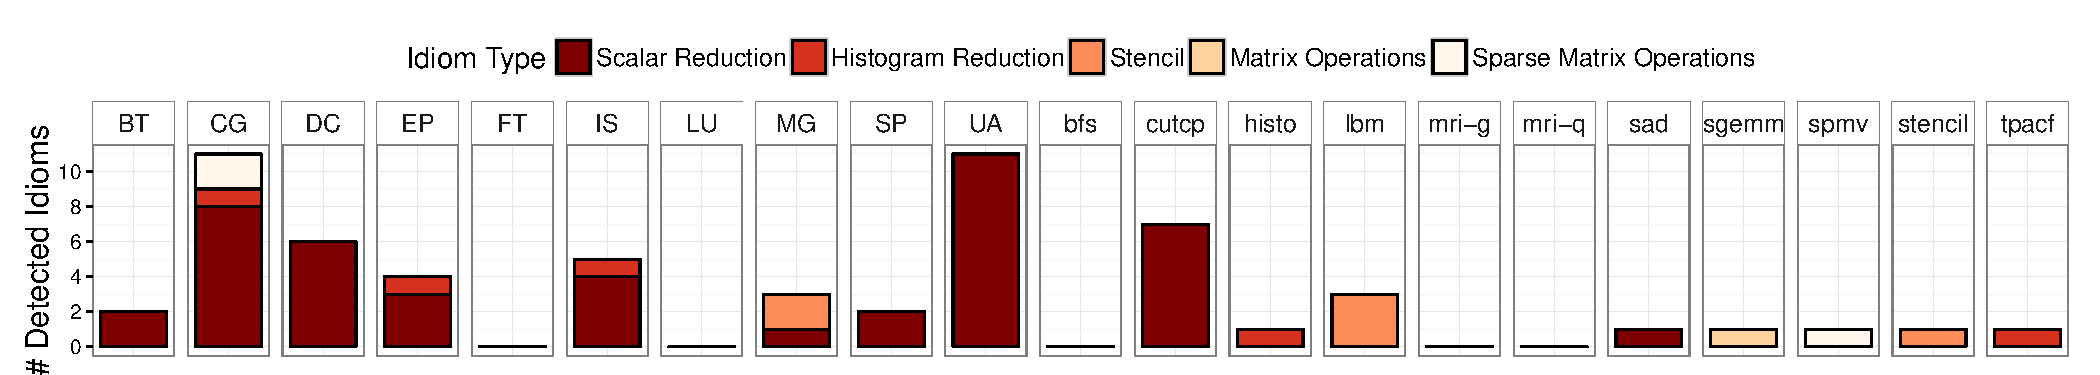
\includegraphics[width=\textwidth]{figures/asplos_detection.pdf}
  \caption{The different computational idioms found across the benchmark
           programs:
           Scalar reductions were the most common, with 10 out of 21 programs
           containing some.
           Other idioms were found in 1--5 programs each.
           Only five of the benchmarks contained no idiomatic code.}
  \label{detection-figure}
\end{figure}
\begin{figure}[p]
  \centering
  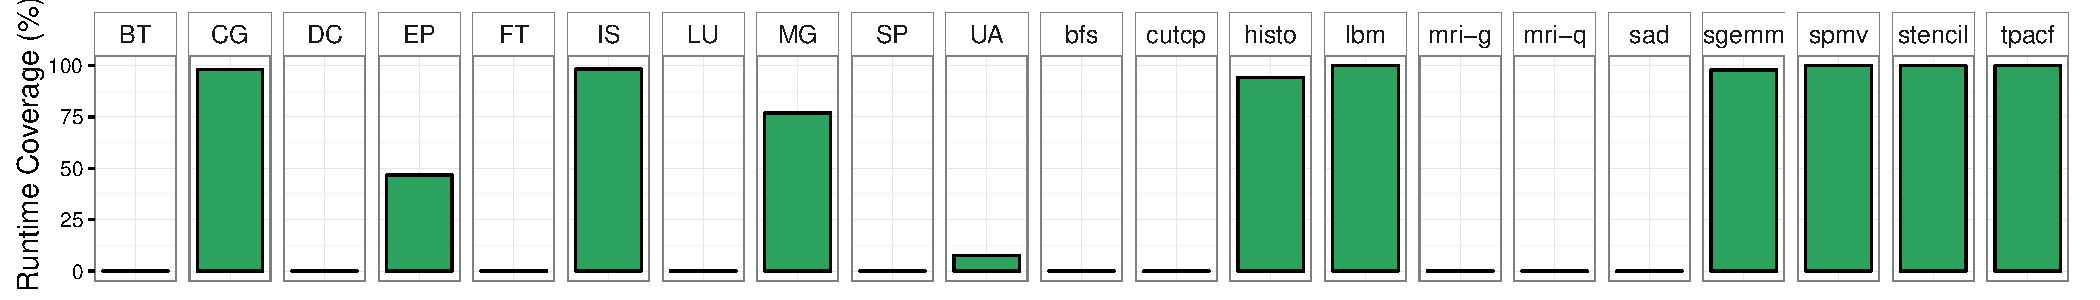
\includegraphics[width=\textwidth]{figures/asplos_coverage.pdf}
  \caption{Runtime coverage: 10 of the 21 programs have idiomatic performance
           bottlenecks.\leftskip=0pt\rightskip=0pt}
  \label{coverage-figure}
  \vspace{0.5em}
\end{figure}

\begin{table}[p]
\centering
  \begin{tabular}{lP{2.16cm}P{2.16cm}P{2.16cm}P{2.163cm}P{2.163cm}}
  \toprule
  \hspace{1.18cm} & Scalar\newline{}Reduction & Histogram\newline{}Reduction & Stencil & Matrix~Op. & Sparse\newline{}Matrix~Op.\\
  \midrule
  Polly &  3  &  --- &   5  &   1  & --- \\
  ICC   &  28 &  --- &  --- &  --- & --- \\
  IDL   &  45 &   5  &   6  &   1  &  3  \\
  \bottomrule
\end{tabular}
\caption{Idioms detected by IDL, ICC, Polly}
\label{tab:detection}
\end{table}

\begin{table}[p]
\centering
\begin{tabular}{lcccccccccccc}
  \toprule
  & \hspace{0.17mm}BT\hspace{0.17mm}
  & \hspace{0.17mm}CG\hspace{0.17mm}
  & \hspace{0.17mm}DC\hspace{0.17mm}
  & \hspace{0.17mm}EP\hspace{0.17mm}
  & \hspace{0.17mm}FT\hspace{0.17mm}
  & \hspace{0.17mm}IS\hspace{0.17mm}
  & \hspace{0.17mm}LU\hspace{0.17mm}
  & \hspace{0.17mm}MG\hspace{0.17mm}
  & \hspace{0.17mm}SP\hspace{0.17mm}
  & \hspace{0.17mm}UA\hspace{0.17mm}
  & \hspace{0.17mm}bfs\hspace{0.17mm}
  & \hspace{0.17mm}cutcp\hspace{0.17mm} \\
  \midrule
without IDL    & 1.9 & 0.5 & 1.0 & 0.3 & 0.6 & 0.3 & 1.9 & 0.8 & 1.6 & 2.7 & 0.4 & 0.4 \\[0.25em]
with IDL       & 4.0 & 0.8 & 1.6 & 0.6 & 1.2 & 0.5 & 3.9 & 4.5 & 3.2 & 7.3 & 0.5 & 0.6 \\[0.75em]
overhead in \% & 116 &  77 &  57 &  77 &  93 &  62 & 103 & 484 &  97 & 169 &  30 &  65 \\
  \bottomrule
\end{tabular}
\begin{tabular}{lccccccccc}
  \toprule
  & \hspace{0.44mm}histo\hspace{0.44mm}
  & \hspace{0.44mm}lbm\hspace{0.44mm}
  & \hspace{0.44mm}mri-g\hspace{0.44mm}
  & \hspace{0.44mm}mri-q\hspace{0.44mm}
  & \hspace{0.44mm}sad\hspace{0.44mm}
  & \hspace{0.44mm}sgemm\hspace{0.44mm}
  & \hspace{0.44mm}spmv\hspace{0.44mm}
  & \hspace{0.44mm}stencil\hspace{0.44mm}
  & \hspace{0.44mm}tpacf\hspace{0.44mm} \\
  \midrule
without IDL    & 0.2 & 0.3 & 0.2 & 0.2 & 0.4 & 0.6 & 0.3 & 0.2 & 0.2 \\[0.25em]
with IDL       & 0.2 & 0.6 & 0.4 & 0.3 & 0.6 & 0.7 & 0.7 & 0.2 & 0.4 \\[0.75em]
overhead in \% &  35 &  87 & 100 &  52 &  58 &  24 & 115 &  36 &  54 \\
  \bottomrule
\end{tabular}
\caption{Compile time cost in seconds}
\label{tab:compiletimecost}
\end{table}

\subsection{Runtime Coverage}

    To determine if the detected idioms were impactful, \Cref{coverage-figure}
    shows the percentage of runtime spent in the detected computational idiom
    for each benchmark program.
    This data shows that either the detected idioms have a low runtime
    contribution or they dominate almost the entire execution.
    \emph{EP} is the only exception with ${\sim}50\%$ runtime coverage.
    Heterogeneous acceleration was evaluated on the ten programs that spend a
    significant amount of time in the detected idioms.
    Only these can reasonably expect a performance gain.

\subsection{Performance Results}

\paragraph*{Speedup over Sequential}

    \Cref{fig:speedup-figure} shows the end-to-end speedup obtained by
    accelerating idioms via heterogeneous APIs on a CPU, an integrated GPU,
    an external GPU, respectively.
    All of the results include data transfer overhead to and from the GPUs,
    where required.
    This overhead is intrinsic to the external GPU, which operates on distinct
    physical memory.
    The integrated GPU, on the other hand, only incurs this cost when APIs
    enforce additional data copies.
    Each bar shows the best-performing API for the given platform;
    \Cref{tab:detailed-results} provides detailed results also for the other
    API backends.

\begin{figure}[t]
  \centering
  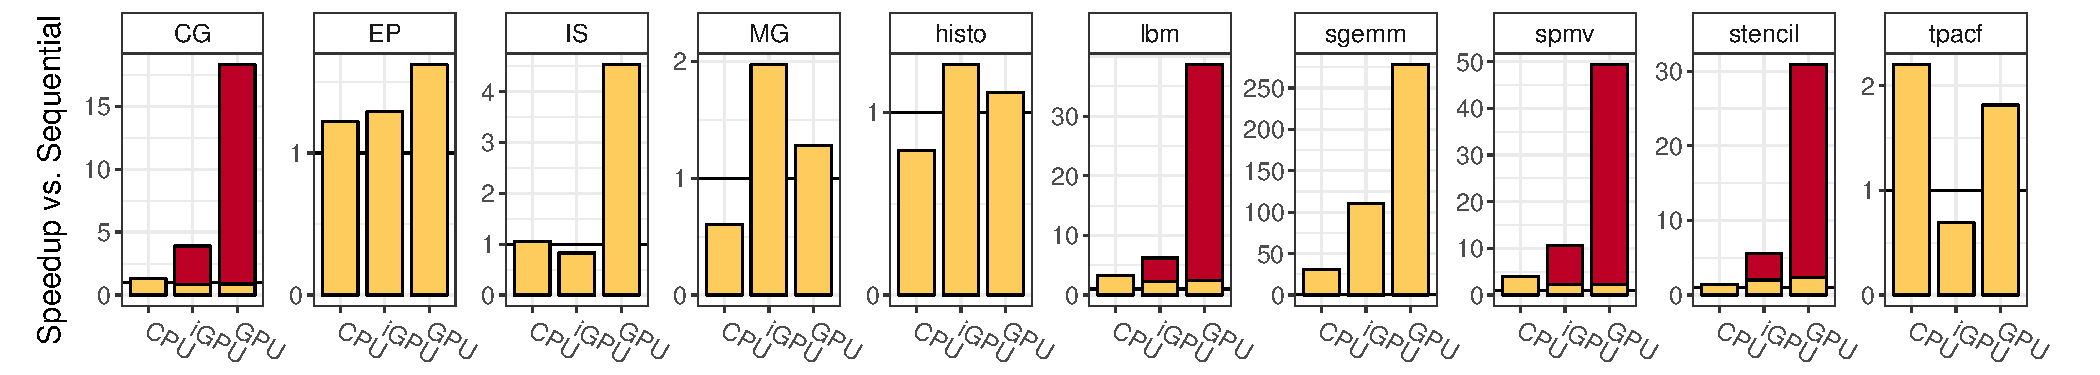
\includegraphics[width=\textwidth]{figures/asplos_speedup.pdf}
  \caption{Speedup over sequential:
           Results for the best-performing backend on each platform are shown.
           The red bars indicate a manual modification for minimising redundant
           data transfers.}
  \label{fig:speedup-figure}
  \vspace{1.5em}
  \centering
  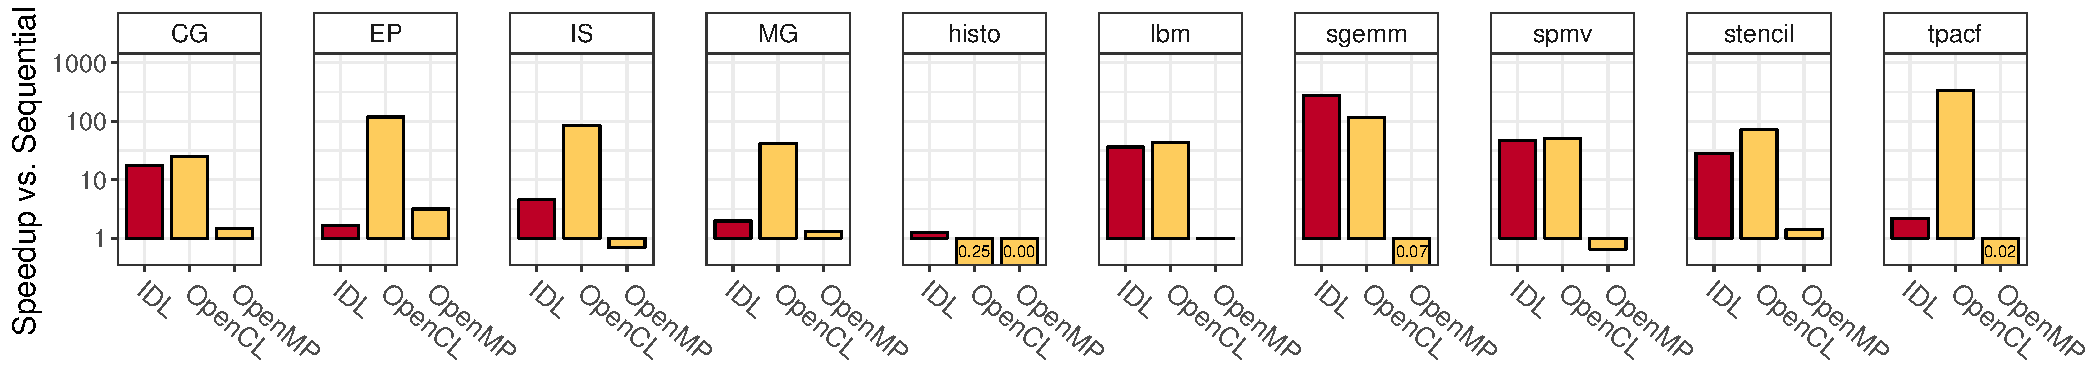
\includegraphics[width=\textwidth]{figures/asplos_comparison.pdf}
  \caption{IDL versus manual expert parallelisation:
           Speedup over the sequential baseline was measured for IDL
           (selecting best performing backend; red bars) and the
           handwritten reference OpenCL and OpenMP implementations
           (provided by the benchmark developers; yellow bars).}
  \label{fig:speedup-figure-2}
  \vspace{0.5em}
\end{figure}

    Moderate speedups were obtained for five of the benchmarks, from
    1.26$\times$ for ``\emph{histo}'' up to 4.5$\times$ for `\emph{IS}''.
    Besides ``\emph{MG}'', all of these benchmarks have a scalar or histogram
    reduction as their performance bottleneck.
    Interestingly, it emerges that for different benchmarks, different hardware
    is beneficial.
    For ``\emph{tpcaf}'', the CPU is the best platform, beating the GPU,
    for which the data transfer time dominates;
    for ``\emph{MG}'' and ``\emph{histo}'', the integrated GPU strikes the right
    balance between computational power and avoiding data movement to the
    external GPU;
    and for ``\emph{EP}'' and ``\emph{IS}'', the data transfer to the GPU is
    amortised by its superior raw performance.
    The results emphasise the significance of flexible heterogeneous
    code generation.
    Committing to any one of the three hardware platforms in the source code
    would have necessarily resulted in less-than-optimal performance for at
    least some of the programs.

    For five of the benchmarks, IDL enabled significantly higher performance
    gains, from 17$\times$ for ``\emph{CG}'' and up to over 275$\times$ for
    ``\emph{sgemm}''.
    These benchmarks are computationally expensive, and the external GPU is
    always the fastest architecture by a considerable margin.

\begin{landscape}
\newlength{\txtwd}
\newcommand{\msb}[1]{\settowidth{\txtwd}{#1}{\tiny\ttfamily\bfseries \hfill #1}}
\newcommand{\ms}[1]{\settowidth{\txtwd}{#1}{\tiny\ttfamily \hfill #1}}
\addtolength{\tabcolsep}{-0.64mm}
\begin{table}[p]
  \centering
  \small
  \begin{tabular}{l|cccccc|ccccc|cccc}
  \toprule
  & \multicolumn{6}{c|}{\bfseries\large CPU} & \multicolumn{5}{c|}{\bfseries\large iGPU} & \multicolumn{4}{c}{\bfseries\large GPU} \\
  & MKL & libSPMV & Halide & clBLAS & CLBlast & Lift & clSPARSE & libSPMV & clBLAS & CLBlast & Lift & cuSPARSE & libSPMV & cuBLAS & Lift \\
  \midrule
   CG      & \msb{1504.21} & --- & --- & --- & --- & --- & \msb{644.02} & --- & --- & --- & --- &  \msb{113.51} & --- & --- & --- \\[3mm]
   EP      & --- & --- & --- & --- & --- &  \msb{32762.50}  & --- & --- & --- & --- & \msb{30983.40}  & --- & --- & --- & \msb{24680.70} \\[3mm]
   IS      & --- & --- & \msb{426.95} & ---  & --- & \ms{1765.61}  &  --- & --- & --- & --- & \msb{547.28}  & --- & --- & --- & \msb{99.95} \\[3mm]
   MG      & --- & --- & --- & --- & --- &  \msb{4699.63}  & --- & --- & --- & --- & \msb{1439.58}  & --- & --- & --- & \msb{2211.56} \\[3mm]
   histo   & --- & --- & --- & --- & --- &  \msb{27.42}  & --- & --- & --- & --- & \msb{17.20}  & --- & --- & --- & \msb{19.54} \\[3mm]
   lbm     & --- & --- & --- & --- & --- &  \msb{6457.93}  & --- & --- & --- & --- & \msb{5335.09}  & --- & --- & --- & \msb{590.60} \\[3mm]
   sgemm   & \msb{53.50} & --- & --- & \ms{1661.75} & \ms{660.44} & \ms{1339.15}  & --- & --- & \msb{14.73} & \ms{19.03} & \ms{15.04}  & --- & --- & \msb{5.99} & \ms{7.87} \\[3mm]
   spmv    & --- & \msb{218.17} & --- & --- & --- & --- & --- &\msb{102.233} & --- & --- & --- & --- &\msb{18.437} & --- &  ---\\[3mm]
   stencil & --- & ---& \msb{5760.81} & --- & --- & \ms{21951.80}  & --- & ---& --- & --- & \msb{2261.48} & --- & ---& --- & \msb{279.38} \\[3mm]
   tpacf   & --- & ---& --- & --- & --- & \msb{19276.40}  & --- & ---& --- & --- & \msb{61111.90} & --- & ---& --- & \msb{23358.20} \\
  \bottomrule
\end{tabular}
\caption{Detailed performance results for each heterogeneous backend interface:
         The runtime of each benchmark program was measured in milliseconds for
         every compatible combination on each of the three platforms.
         The fastest implementations per benchmark and target hardware are
         highlighted in {\bf bold}.}
\label{tab:detailed-results}
\end{table}
\end{landscape}

    The red highlighting in \Cref{fig:speedup-figure} indicates an important
    runtime optimisation:
    Redundant data transfers for the iterative ``\emph{CG}'', ``\emph{lbm}'',
    ``\emph{spmv}'' and ``\emph{stencil}'' benchmarks were manually eliminated.
    All of these benchmarks execute computations inside a for-loop and do not
    require access to the data on the CPU between iterations.
    A straightforward lazy copying technique was manually applied by flagging
    memory objects to avoid redundant transfers, similar
    to work by \citet{jablin11automatic}.
    This runtime optimisation is crucial for achieving high performance on some
    of the benchmark programs.

\paragraph*{API performance comparison}

    \Cref{tab:detailed-results} shows a breakdown of the performance of each API
    on each program and platform.
    Not all APIs target all platforms, {\emph{e.g.} cuSPARSE only targets NVIDIA
    GPUs.
    The version of Halide that was used for this evaluation failed to generate
    valid GPU code for any of the benchmarks.
    Therefore, only the CPU platform was evaluated with Halide.
    The best-performing backend is highlighted in bold in the table entries.
    None of the previously existing backends supported SPMV-JDS, which was used
    by the ``\emph{spmv}'' benchmark.
    The libSPMV library was implemented as an ad-hoc solution to this,
    providing straightforward parallelisation of the idiom.

    On the multi-core CPU, Intel MKL gave the best linear algebra performance,
    outperforming the other libraries and Lift.
    Halide achieved good performance for the NPB ``\emph{IS}'' and Parboil
    ``\emph{stencil}'' benchmarks on the CPU, outperforming Lift due to its more
    advanced vectorisation capabilities.
    In programs that were dominated by scalar reductions, Lift performed well.
    On the internal GPU, clBLAS provides a better matrix-multiplication
    implementation than either CLBlast or Lift.
    On the external GPUs, library backends provided the best linear algebra
    implementations, while Lift performed well on stencils and reductions.

\paragraph*{Speedup vs Handwritten Parallel Implementations}

    \Cref{fig:speedup-figure-2} shows the performance of the IDL approach
    compared to handwritten reference OpenMP and OpenCL implementations.
    For some of the benchmarks, the parallel versions are significantly modified
    and use different algorithms beyond the reach of automation.
    For benchmarks where the parallel reference implementation does not make
    profound algorithmic changes (``\emph{CG}'', ``\emph{histo}'',
    ``\emph{lbm}'', ``\emph{sgemm}'', ``\emph{spmv}'', ``\emph{stencil}''),
    IDL enabled comparable -- or better -- performance.
    For four benchmarks (``\emph{EP}'', ``\emph{IS}'', ``\emph{MG}'',
   ``\emph{tpacf}'') it is beneficial to parallelise the entire application,
    which is beyond the scope of this work.

    The handwritten versions of ``\emph{sgemm}'' and ``\emph{stencil}' were
    outperformed by IDL.
    This was due to implementation flaws; a loop interchange already improved
    performance by almost 20$\times$.

\paragraph*{Summary}

    60 idioms were detected across the benchmark suites, and significant
    performance improvements were achieved by targeting different heterogeneous
    APIs for those benchmarks where idioms dominate execution time.

\section{Conclusions}

    The chapter developed a compiler-based approach that automatically detects
    a broad class of computational idioms that are supported by libraries or
    domain-specific languages targeting heterogeneous computing.
    The approach is based on the declarative Idiom Detection Language that
    identifies program subsets adhering to idiom specifications with a
    constraint solver.
    Once detected, the idiomatic loops were mechanically translated into API
    calls to external libraries or to code generated by DSL compilers.

    The approach was evaluated on the C/C++ programs from two well-known
    benchmark suites: NAS and Parboil.
    IDL detected more stencils, sparse matrix operations and generalised
    reduction and histogram computations than existing approaches, and generated
    fast code.


\chapter[Building a Fully integrated Idiom Specific Optimization Pipeline]
        {Building a Fully integrated Idiom Specific Optimization Pipeline
         \footnote{This chapter is based on published research in
                   \citet{lilacpaper}.}}
    \label{chapter:lilac}
     
    Sparse linear algebra is central to many scientific codes, yet compilers
    fail to optimize it well.
    Instead, programmers rely on library implementations that are hand optimized
    and can utilize accelerator hardware.
    This comes at a cost, however, as it ties programs into vendor specific
    software ecosystems and results in non-portable code.

    This chapter develops an approach based on the {\em specification
    Language for implementers of Linear Algebra Computations} (LiLAC).
    Rather than requiring application developers to (re)write every program for
    a given library, the burden is shifted to a {\em one-off} description for
    the library implementer.
    The LiLAC-enabled compiler then uses this to incorporate library routines
    automatically.

    LiLAC provides automatic data marshaling, seamlessly maintaining state
    between calls as needed and minimizing data transfers.
    Appropriate places for library replacement are detected at the compiler
    intermediate representation level, making our approach language independent.

    We evaluate on legacy large-scale scientific applications written in FORTRAN;
    standard benchmarks written in C/C++ and FORTRAN; and C++ graph analytics kernels.
    Across heterogeneous platforms, applications and data sets we show performance
    improvements of 1.1x to over 10x without any user intervention.


\section{Introduction}

    Linear algebra is an important component of many compute intensive
    applications.
    While there are many compiler papers examining automatic optimization of
    dense linear algebra, sparse codes have received less attention. 
    Sparse algorithms are, however, increasingly important as the basis for
    graph algorithms and data analytics \cite{Kepner2015GraphsMA}.

Ideally, we would like compilers to automatically map dense and sparse-based
codes to heterogeneous compute platforms efficiently and with no user
intervention. However,  this has proven difficult.

Instead, we see the wide-scale provision of fast libraries
\cite{cusparse,clsparse,mkl}, often provided by hardware vendors themselves.
They provide excellent performance, but place the burden of code rewriting on
the application developer and are rarely portable across platforms.
Rewriting legacy applications involves considerable effort, especially when
using hardware accelerators that require careful data marshaling.
In fact, the difficulty of efficient integration is a key impediment to the
wider use of accelerator libraries.
Furthermore, source code modifications reduce the portability of the
program and require a commitment to specific hardware vendors, resulting in legacy
code bases that quickly become obsolete.

In this chapter, we reexamine the way that compilers and libraries are used
to tackle the challenge of achieving full performance without requiring any
application programmer effort.
Highly tuned and platform specific libraries are invariably the fastest
implementations available, therefore we use them as our building blocks.
We then develop a new specification language for implementers of such
libraries, the {\em specification Language for implementers of Linear Algebra
Computations} (LiLAC).

Using LiLAC, library implementers specify with a few lines of code,
{\em what} a library does and {\em how} it is invoked.  Our compiler
then determines where the library specification matches the user's
code and automatically rewrites the code to utilize library calls.

\paragraph*{LiLAC-What}
is a high level language to describe sparse and dense linear
algebra programs.
The LiLAC compiler uses it to detect such functionality
in user applications at the level of compiler intermediate representation.
It is powerful enough to formulate linear algebra, yet remains
independent of compiler internals and is easy to understand and program.

\paragraph*{LiLAC-How}
is a language to specify how parts of the LiLAC-What description
can be used for library invocations and how state can be retained in between
calls.
Our compiler uses this to automatically generate library call {\em harnesses} that
efficiently schedule memory transfers, execute setup code and handle hardware
context management.

Our approach is broadly applicable. To demonstrate its applicability
to legacy FORTRAN codes, we improved and extended the flang frontend
to LLVM and evaluated on a large-scale scientific application.
It also works on standard C/C++ and FORTRAN benchmark programs and C++ graph
\mbox{analytics} kernels. The presented LiLAC system achieves significant performance
improvement across heterogeneous platforms, from 1.1x to over 10x, without any
user intervention.

\begin{figure*}[t]
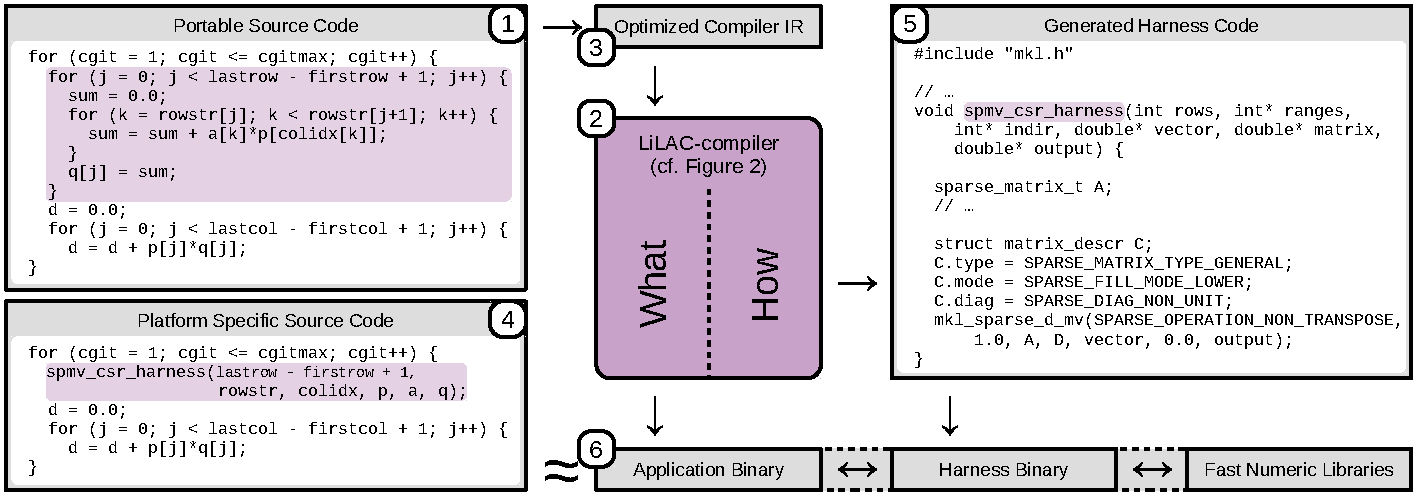
\includegraphics[width=\textwidth]{figures/lilac_overview.pdf}
\caption{LiLAC applied to NPB Conjugate Gradient:
         Code that matches the LiLAC-What specification is replaced with calls
         to a harness function. The harness is generated from a LiLAC-How
         specification to utilize Intel MKL.}
\label{motivationcode}
\end{figure*}

\section{Overview}
\label{sec:overview}

Consider the example in \autoref{motivationcode}.  In the top left
corner (1), we see unmodified application source code.  This is
{\em conjugate gradient} from the NAS-PB suite.  The program is written
in a straightforward manner and a naively compiled program would fail
to exploit the full potential of modern hardware.

In order to achieve good performance on Intel processors, we provide a
LiLAC specification of Intel MKL.
The LiLAC compiler (2) uses this to detect that the code in the framed loop is a
sparse matrix-vector product.
Instead of passing it on to the generic compiler backend, it replaces it with a
call to an auto-generated {\em harness} function  and captures the parameters of the computation
as function call arguments.
This is performed on optimized intermediate representation code (3)
and results in a program that is equivalent to the source code shown in the
bottom left (4).

LiLAC also automatically generates the corresponding harness as shown at
the right of the figure (5).
The resulting shared library is then linked with the application binary at
runtime, interfacing the underlying library implementation (6).

\begin{figure*}[t]
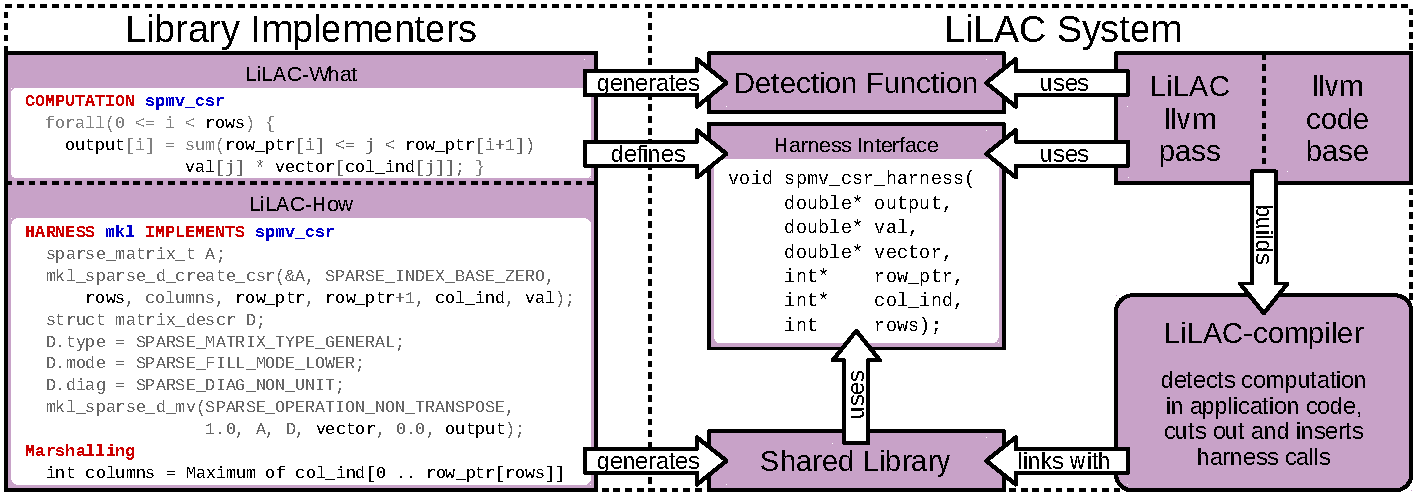
\includegraphics[width=\textwidth]{figures/whathowflow.pdf}
\caption{Overview of the LiLAC internals: On the left is the entire LiLAC
         program the library implementer must write. This results in a modified
         LiLAC-compiler in the bottom right that behaves as the shown in
         \autoref{motivationcode}.}
\label{motivationflow}
\end{figure*}

\subsection{Implementation Overview}

\autoref{motivationflow} provides more detail on the internals of
LiLAC.  On the left we can see the LiLAC specification provided by the
library implementer - just 16 lines of code.  It consists of a
{\em What} and a {\em How} part.  These two parts are processed by the
LiLAC system, eventually resulting in a runtime library and a modified
C/C++ compiler.

{\bf LiLAC-What} specifies the functionality that is provided by a library,
in this example {\em spmv-csr} (cf.\ \autoref{motivationcode}).
From this specification, a detection program that finds the computation in
normalized LLVM IR code is automatically generated and the harness interface
is determined.

{\bf LiLAC-How} specifies how the library, in this case Intel MKL, can be
invoked to perform the specified calculation.
This involves boilerplate code, but also advanced features, such as optimized
data transfers to accelerators.
In the last two lines, we can see how to efficiently compute the {\em columns}
variable with LiLAC.
It is not present in the {\em LiLAC-What} definition but is required by the MKL library. It  cannot be
captured statically and has to be computed at runtime using the values in the
{\em row\_ptr} array.
Using {\em Marshalling}, LiLAC automatically generates the harness
such that this is only recomputed if the values in {\em row\_ptr} change.

On the right of the figure we can see how the components generated from the
LiLAC specification are used to build the LiLAC-compiler.
Based on the LLVM infrastructure, it implements a transformation pass that
is executed after the normal optimization pipeline.
Using the generated detection function, it finds instances of the computation
and replaces them with calls to the specified harness interface.
Application binaries are dynamically linked to the harness library.

\section{What and How}

This section describes in more detail the two components of the LiLAC language.
LiLAC-What describes what a specific library does and LiLAC-How describes how
user code is bound to the underlying implementation.

\subsection{LiLAC-What: Functional Description}
At the heart of our approach is a simple language to specify sparse and dense
linear algebra operations.
This serves two purposes in our LiLAC system: Firstly, it is used to generate
a detection program for finding the computation in user code.
Secondly, it identifies the variables that are arguments to the library, thus
defining the harness interface.

The key challenge in the design of this language was to stay simple enough
to allow automatic generation of robust detection functionality, yet to be able
to capture interesting functionality.
Crucial for sparse linear algebra routines is capturing the many different
memory access patterns, the control flow on the other hand is very rigid.
This is reflected in the grammar as shown in \autoref{bnfgrammar}.

\subsection{Sparse Matrix Variations in LiLAC-What}
Sparse matrices can be stored in different formats.
In this section we introduce two of them and show how LiLAC-What can express
the corresponding computations.

\begin{figure}[t]
\begin{align*}
program ::=\ &\textbf{COMPUTATION} \left<name\right> \left<body\right>\\
body    ::=\ &\left<forall\right> \mid \left<dotop\right>\\
range   ::=\ &\textbf{(} \left<exp\right> \textbf{<=} \left<name\right> \textbf{<} \left<exp\right> \textbf{)}\\
forall ::=\ &\textbf{forall} \left<range\right> \textbf{\{} \left<body\right> \textbf{\}}\\
dotp    ::=\ &\left<addr\right> \textbf{=}\ \textbf{dot} \left<range\right> \left<addr\right> \textbf{*} \left<addr\right> \textbf{;}\\
addr    ::=\ &\left<name\right> \{\ \textbf{[} \left<exp\right> \textbf{]}\ \}\\
add     ::=\ &\left<exp\right> \textbf{+} \left<exp\right>\\
mul     ::=\ &\left<exp\right> \textbf{*} \left<exp\right>\\
exp     ::=\ &\left<name\right> \mid \left<cnst\right> \mid \left<addr\right> \mid\ \left<add\right> \mid \left<mul\right>
\end{align*}
\vspace{-1.5em}
\caption{Grammar of the LiLAC-What language}
\label{bnfgrammar}
\end{figure}

\begin{figure}[t]
\begin{minipage}[b]{0.3\linewidth}
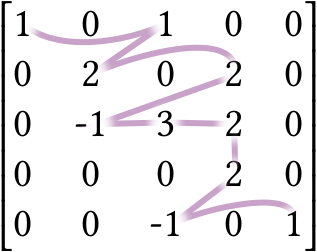
\includegraphics[width=0.9\linewidth]{figures/csrorder.png}
\vspace{0.04em}
\end{minipage}
\begin{minipage}[b]{0.65\linewidth}
\begin{align*}
\text{\bf val} =& \begin{bmatrix}
1\ \ 1\ \ 2\ \ 2\ \ \text{-}1\ \ 3\ \ 2\ \ 2\ \ \text{-}1\ \ 1\\
\end{bmatrix}\\
\text{\bf col\_ind} =& \begin{bmatrix}
0\ \ 2\ \ 1\ \ 3\ \ 1\ \ 2\ \ 3\ \ 3\ \ 2\ \ 4\\
\end{bmatrix}\\
\text{\bf row\_ptr} =& \begin{bmatrix}
0\ \ 2\ \ 4\ \ 7\ \ 8\ \ 10\\
\end{bmatrix}
\end{align*}
\end{minipage}
\caption{Compressed Sparse Row representation as used by the LiLAC-What example
         in \autoref{motivationcode}}
\label{csr_lilacwhat_fig}
\vspace{1.5em}
\centering
\begin{minipage}[b]{0.3\linewidth}
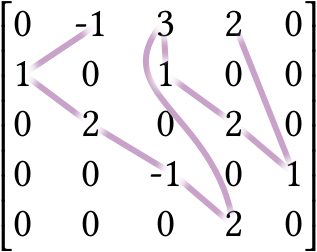
\includegraphics[width=0.9\linewidth]{figures/jdsorder.png}
\vspace{0.04em}
\end{minipage}
\begin{minipage}[b]{0.65\linewidth}
\footnotesize
\begin{align*}
\text{\bf perm} =& \begin{bmatrix}1\ \ 2\ \ 0\ \ 4\ \ 3\\\end{bmatrix}\\[-0.4em]
\text{\bf val} =& \begin{bmatrix}\text{-}1\ \ 1\ \ 2\ \ \text{-}1\ \ 2\ \ 3\ \ 1\ \ 2\ \ 1\ \ 2\\\end{bmatrix}\\[-0.4em]
\text{\bf col\_ind} =& \begin{bmatrix}1\ \ 0\ \ 1\ \ 2\ \ 3\ \ 2\ \ 2\ \ 3\ \ 4\ \ 3\\\end{bmatrix}\\[-0.4em]
\text{\bf jd\_ptr} =& \begin{bmatrix}0\ \ 5\ \ 9\ \ 10\\\end{bmatrix}\\[-0.4em]
\text{\bf nzcnt} =& \begin{bmatrix}3\ \ 2\ \ 2\ \ 2\ \ 1\end{bmatrix}
\end{align*}
\end{minipage}
\vspace{0.5em}
\hrule
\vspace{0.3em}
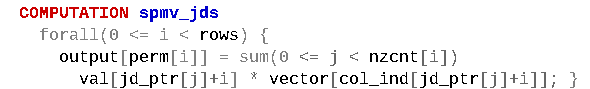
\includegraphics[width=\linewidth]{figures/spmvjdswhat.pdf}
\vspace{-1.2em}
\caption{Jagged Diagonal Storage in LiLAC-What}
\label{jds_lilacwhat_fig}
\end{figure}

\subsubsection{Compressed Sparse Row}
For Compressed Sparse Row (CSR) \cite{doi:10.1137/1.9780898718003}, all non-zero
entries are stored in a flat array \textbf{val}.
The \textbf{col\_ind} array stores the column position for each value.
Finally, the \textbf{row\_ptr} array stores the beginning of each row of the
matrix as an offset into the other two arrays.
The number of rows in the matrix is given directly by the length of the
\textbf{row\_ptr} array minus one, however the number of columns is not
explicitly stored.
In \autoref{csr_lilacwhat_fig}, a 5x5 matrix is shown represented in this
format, the LiLAC-What code is in the top left of \autoref{motivationflow}.

\subsubsection{Jagged Diagonal Storage}
For Jagged Diagonal Storage (JDS) \cite{doi:10.1137/0910073}, the rows of the
matrix are permuted such that the number of nonzeros  per row  decreases. The
permutation is stored in a vector \textbf{perm}, the number of nonzeros in
\textbf{nzcnt}.
The nonzero entries are then stored in an array \textbf{val} in the following
order: The first nonzero entry in each row, then the second nonzero entry in
each row etc.
The array \textbf{col\_ind} stores the column for each of the values and
\textbf{jd\_ptr} stores offsets into \textbf{val} and \textbf{col\_idx}.
The product of a sparse matrix in JDS format with a dense vector is specified 
in LiLAC-What at the bottom of \autoref{jds_lilacwhat_fig}.

\subsection{LiLAC-How}
\label{sec:lilachow}

    Where LiLAC-What specifies the computations that are implemented by a
    library, LiLAC-How describes how precisely library calls are to be be used
    for performing them.
    The langauge was designed with important existing libraries such as 
    cuSPARSE, clBLAS and Intel MKL in mind.
    In order to support the idiosyncrasies of these libraries, the
    specifications need to be built around boilerplate C++ code that manages the
    construction of parameter structures, calling conventions etc.
    However, it is also crucial for the specification language to be as
    high-level as as possible without sacrificing any performance, and the fine
    balance between these requirements drove the design of the language.
    In particular, LiLAC-How abstracts away memory transfers.

    The result is a language that can be further divided into two interacting
    components.
    Firstly, it describes boilerplate code that is required for individual library
    call invocations in a {\em harness}.
    Secondly, it is used for data {\em marshaling} between the core program and the
    library, which is particularly crucial for heterogeneous compute environments.
    \autoref{lilacbnf2} shows the grammar specification of LiLAC-How.

\subsubsection{Individual Library Invocations}
We need to encapsulate the boilerplate code that any given library requires,
such as setup code, filling of parameter structures etc.
This part of the language is straightforward.

\paragraph{Harness}
The harness construct is the central way of telling the LiLAC system how a
library can be used to perform a computation that was specified in LiLAC-What.
As we can see at the top of \autoref{lilacbnf2}, a harness refers to a
LiLAC-What program by name and also has a name itself.
It is built around some C++ code, which can use all the variables from the
LiLAC-What program to connect with the surrounding program.
It also needs to specify the relevant C++ header files
that the underlying library requires.
Lastly, the harness can incorporate persistent state and utilize data
marshaling functionality.

\paragraph{Persistence}
Many libraries need setup and cleanup code, which is specified with the
keywords {\em BeforeFirstExecution} and {\em AfterLastExecution}.
These are used in combination with {\em PersistentVariables}, allowing state to
persist between harness invocations, e.g.\ to retain handlers to hardware
accelerators.

\paragraph{Example}
In \autoref{mklharness1}, we see a trivial LiLAC-What program for implementing
\texttt{spmv\_csr} with the Intel MKL library.
The actual call to the relevant library function is in line 16.
To prepare for that call, there is boilerplate code in lines 7--14 to fill
parameter structures.

Critically, there is an additional parameter required by the library that is
not part of the LiLAC-What specification: the number of columns, {\em cols}, in
the sparse matrix.
It is determined at runtime, in lines 2--5, leading to reduced performance.
We will avoid this with the data marshaling constructs in the next section.

\subsubsection{Data Marshaling}
Heterogeneous accelerators require data transfers to keep memory consistent
between host device and accelerator.
To achieve the best performance, these have to be minimized.

Importantly, unchanged data should never be copied again.
This is not trivial to achieve, as it requires dynamic checks.
LiLAC-How uses hardware memory protection to implement this with minimal
run time overhead in generated harnesses.

\begin{figure}[t]
\centering
\begin{align*}
harness  ::=\ &\textbf{HARNESS} \left<name\right> \textbf{IMPLEMENTS} \left<name\right>\\[-0.3em]
              &\left<C++\right>\\[-0.3em]
           [\ &\left<marshalling\right>\ ]\ [\ \left<persistence\right> ]\\[-0.3em]
           [\ &\textbf{CppHeaderFiles}\ \{\ \left<name\right>\ \}\ ]\\
persistence ::=\ &\textbf{PersistentVariables}\ \{\ \left<name\right> \left<name\right>\ \}\\[-0.3em]
              [\ &\textbf{BeforeFirstExecution} \left<C++\right>\ ]\\[-0.3em]
              [\ &\textbf{AfterLastExecution} \left<C++\right>\ ]\\[-1em]
\cline{1-2}\\[-2em]
marshalling ::=\ &\textbf{Marshalling}\\[-0.3em]
          \{\ &\left<type\right> \left<name\right> \textbf{=} \left<name\right> \textbf{of}\\[-0.3em]
              &\left<name\right>\ \textbf{[}\ \textbf{0}\ \textbf{..} \left<exp\right> \textbf{]}\ \}\\
input   ::=\ &\textbf{INPUT} \left<name\right> \left<C++\right>\\[-0.3em]
             [\ &\textbf{BeforeFirstExecution} \left<C++\right>\ ]\\[-0.3em]
             [\ &\textbf{AfterLastExecution} \left<C++\right>\ ]\\
output  ::=\ &\textbf{OUTPUT} \left<name\right> \left<C++\right>\\[-0.3em]
             [\ &\textbf{BeforeFirstExecution} \left<C++\right>\ ]\\[-0.3em]
             [\ &\textbf{AfterLastExecution} \left<C++\right>\ ]
\end{align*}
\vspace{-1.5em}
\caption{Grammar of LiLAC-How}
\label{lilacbnf2}
\end{figure}

\begin{figure}[t]
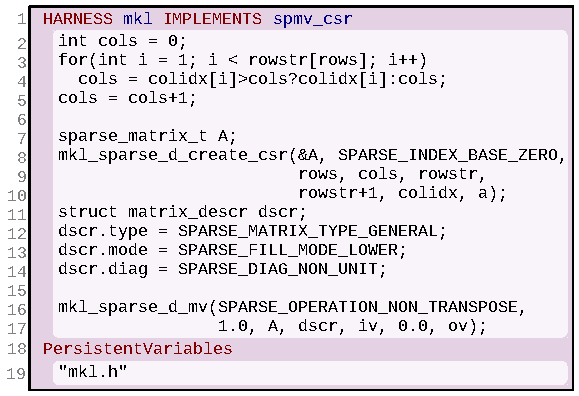
\includegraphics[width=0.944\linewidth]{figures/harness2.pdf}
\\[-0.75em]
\caption{This LiLAC-What code implements CSR SPMV na\"ively with Intel MKL.
         Performance is degraded because of lines 2--5.
         \autoref{readablemax} will present a solution to this bottleneck.}
\vspace{2.em}
\label{mklharness1}
\end{figure}

\begin{figure}[t]
\centering
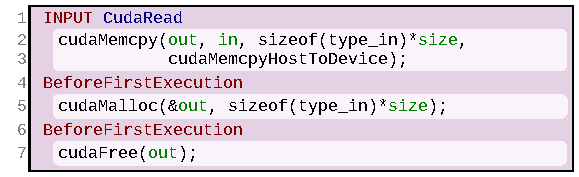
\includegraphics[width=0.944\linewidth]{figures/harness3.pdf}
\\[-0.75em]
\caption{LiLAC-How code to provide efficient automatic data marshaling between
         host and CUDA accelerator.}
\label{cudaread}
\end{figure}

\begin{figure}[t]
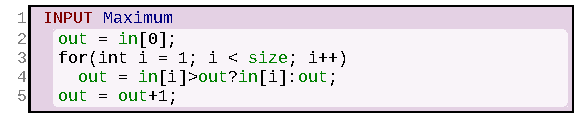
\includegraphics[width=0.944\linewidth]{figures/harness4.pdf}
\\[-0.75em]
\caption{{\em INPUT} can also be used to specify data dependent computations
         that are only recalculated when required.}
\vspace{0.5em}
\label{readablemax}
\end{figure}

\begin{figure}[t]
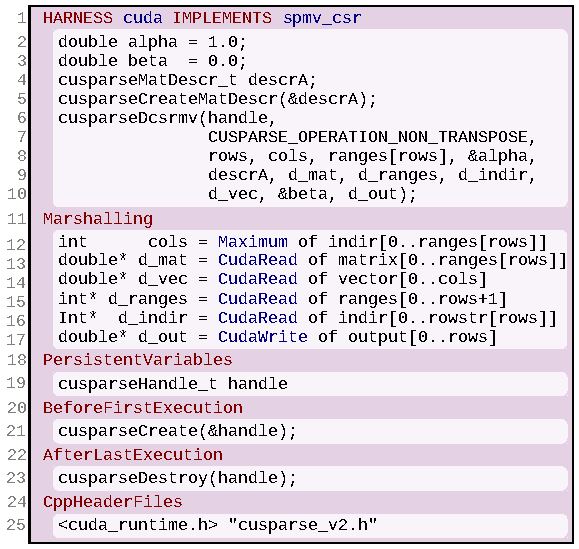
\includegraphics[width=0.944\linewidth]{figures/harness1.pdf}
\\[-0.75em]
\caption{This LiLAC-What specification implements an efficient SPMV harness
  using cuSPARSE in only 25 lines of code.}
\label{spmvharness}
\end{figure}

This data {\em marshaling} comes in two flavors; INPUT and OUTPUT.
Both of these are bound to a range of memory in the harness.
The LiLAC-generated code then uses hardware memory protection to detect read and
write accesses to these memory ranges.
In the specification, the underlying array is available using the
identifiers {\tt in}, {\tt size}, and {\tt out}.

\subsubsection{Detailed Example}
In \autoref{cudaread}, LiLAC-How functionality is specified using the
\texttt{cudaMemcpy} function from NVIDIA CUDA.
It is used to copy data from the host to the accelerator.
Note that for this to work, it first needs to allocate memory of the
device using \texttt{cudaMalloc}, which is later freed with \texttt{cudaFree}.
\texttt{cudaMemcpy} is executed only when a value in the array changes,
resulting in minimal memory transfers.

We can use the same construct to efficiently compute values
such as the \texttt{cols} variable in \autoref{mklharness1}, as shown in
\autoref{readablemax}.
The optimized implementation is nearly identical to the code in
\autoref{mklharness1} lines 2-5, however instead of the concrete variable name
the reserved identifiers {\tt in}, {\tt size}, and {\tt out} are used.
\pagebreak

We can now use these in \autoref{spmvharness}, showing a CSR SPMV
LiLAC-How program for the cuSPARSE library.
A number of data marshaling variables are introduced in lines 12--17, that
automatically optimize both memory transfers and the computation of the
\texttt{cols} variable.
The core of the harness in lines 2--10 is again nothing more than 
library specific boilerplate C++ code.

\section{Implementation}
\label{sec:implementation}

    The LiLAC system, as shown in \autoref{motivationflow} is entirely
    integrated into the LLVM build system.
    When LLVM is compiled, the LiLAC specification is parsed using a Python
    program.
    Based on the LiLAC-What and LiLAC-How sections, C++ code is generated that
    is automatically incorporated into LLVM in further stages of the build
    process.

    The result is an LLVM optimization pass that is available when linking LLVM
    with the clang C/C++ compiler.
    This performs the discovery of linear algebra code and the insertion of
    harness calls.
    Furthermore, the harness libraries themselves are built at compile time of
    LLVM, using C++ code emitted from the LiLAC-How sections.

    The two crucial implementation details are therefore:
    Firstly, how automatic detection functionality in C++ can be generated from
    the abstract LiLAC-What specifications and \linebreak
    secondly, how the LiLAC-How sections are used to generate fast C++
    implementations of the specified library harnesses.

\subsection{LiLAC-What}
Once the LiLAC-What sections have been parsed, they are turned into C++
functionality that is used by the LiLAC LLVM pass to detect appropriate places
for harness calls.
Instead of performing this via syntax-level pattern matching, we use optimized
intermediate compiler representation.
The standard optimizations for \texttt{-O2} without vectorization and loop
unrolling are used.
This results in code in a normal form, which allows us to abstract away many
syntactic differences and programming languages.

The effect is demonstrated in \autoref{robustness}, which shows three
implementations of a dot product in different languages: C, C++ and FORTRAN.
After translating to LLVM IR and performing optimizations, the dot product is
recognized in the LiLAC system using the same LiLAC-What specification.

The exact detection algorithm works in two steps.
Firstly, the control flow skeleton is recognized.
This is simple, as the control flow that can be expressed in LiLAC-What is
limited, and we only need to detect loop nests of a certain depth.
After candidate loop nests have been identified, the index and loop range
calculations from LiLAC-What are mapped onto the LLVM IR nodes.
This is done via a backtracking search procedure that requires some careful
consideration in order to get robust results on implementation details of LLVM,
particularly for different ways of array indexing, pointer casts and integer
conversions.

\subsubsection{Backtracking Search Algorithm}
In order to match instances of LiLAC-What specifications in user programs,
the LLVM IR segments that match the corresponding control flow skeleton are
processed with a backtracking search algorithm.

All $\left<exp\right>$ expressions in the LiLAC-What program are identified.
These now have to be assigned instructions or other values from the LLVM IR
segment. The top-level $\left<exp\right>$ expressions that are used as limits or
iterators in $\left<range\right>$ expressions are easily connected with the
corresponding loop boundaries in the matched control flow structures.

    The remaining expressions are then successively assigned by backtracking.
    Consider the example in \autoref{llvmexample}, which shows a candidate loop
    from the LLVM IR generated from the C++ dot product code in
    \autoref{robustness}.
    The iteration space is determined by loop analysis and this immediately
    allows us to assign the LiLAC-What iterator and range in
    \autoref{backtrack}.
    The LLVM IR instructions that correspond to \texttt{left[i]}, \texttt{left},
    \texttt{right[i]}, \texttt{right} and \texttt{result} are then searched for
    one by one.
    When a partial solution fails, such as at the point when \texttt{right} is
    assigned the same value as \texttt{left}, we backtrack.
    If we cannot determine a solution this way, we discard the control flow
    candidate.

\subsubsection{Code Replacement}

    For each identified loop nest that matches a LiLAC-What specification, the
    code is replaced with a harness call.
    To minimize the invasiveness of our pass, this is performed as follows:
    Firstly, a harness call is inserted directly before the loop.
    The function call arguments are then selected from the backtracking result
    and passed to the harness.
    Secondly, the LLVM instruction that stores the result of the computation or
    passes it out of the loop as a phi node is removed.
    The remainder of the loop nest is be removed automatically by dead code
    elimination.

\begin{figure}[p]
\begin{lstlisting}[language=LiLAC,numbers=none]
COMPUTATION dotproduct
    result = sum(0 <= i < length) left[i] * right[i];
\end{lstlisting}
\begin{lstlisting}[language=C,numbers=none]
int i = 0;
while(i < N) {
    x += (*(A+i))*(*(B+i));
    i+=1; }
\end{lstlisting}
\vspace{-0.75em}
\begin{lstlisting}[language=C++,numbers=none]
for(int i = 0; i < vec_a.size(); i++)
    x += vec_a[i]*vec_b[i];
\end{lstlisting}
\vspace{-0.75em}
\begin{lstlisting}[language=FORTRAN,numbers=none]
DO I = 1, N, 1
    X = X + A(i)*B(i)
END DO
\end{lstlisting}
\vspace{-0.75em}
\caption{Syntactically different computations in C, C++ or FORTRAN are captured
         by one LiLAC-What specification.}
\label{robustness}
\vspace{1em}
\begin{lstlisting}[language=llvm,numbers=none]
; <label>:17:
  %18 = phi i64 [ 0, %10 ], [ %26, %17 ]
  %19 = phi double [ 0.0, %10 ], [ %25, %17 ]
  %20 = getelementptr double, double* %9, i64 %18
  %21 = load double, double* %20
  %22 = getelementptr double, double* %12
  %23 = load double, double* %22
  %24 = fmul double %21, %23
  %25 = fadd double %19, %24
  %26 = add nuw i64 %18, 1
  %27 = icmp ugt i64 %14, %26
  br i1 %27, label %17, label %15
\end{lstlisting}
\vspace{-0.75em}
\caption{Optimizations remove language specific features, the result is
         normalized LLVM IR. Control flow candidates for a match are easily
         determined with standard loop analysis.}
\label{llvmexample}
\vspace{1em}
\begin{tabular}{rcr|rcrr}
       &              &      & left[i]  & $\leftarrow$&                 \%21   &     \\
     i & $\leftarrow$ & \%18 & left     & $\leftarrow$&                  \%9   &     \\
length & $\leftarrow$ & \%14 & right[i] & $\leftarrow$&                 \%21   & \%23\\
       &              &      & right    & $\leftarrow$& \textcolor{red}{fail!} & \%12\\
       &              &      & result   & $\leftarrow$&                        & \%19\\
\end{tabular}
\caption{Control flow candidates contain iterator ranges directly (left),
         backtracking identifies the dot product by assigning the other
         LiLAC-What entities one by one (right).}
\label{backtrack}
\end{figure}

\begin{figure}[t]
\begin{lstlisting}
template<typename type_in, typename type_out>
void CudaRead_update(type_in* in, int size,
                     type_out& out) {
    cudaMemcpy(out, in, sizeof(type_in)*size,
               cudaMemcpyHostToDevice);
}
template<typename type_in, typename type_out>
void CudaRead_construct(int size, type_out& out) {
    cudaMalloc(&out, sizeof(type_in)*size);
}
template<typename type_in, typename type_out>
void CudaRead_destruct(int size, type_out& out) {
    cudaFree(out);
}
template<typename type_in, typename type_out>
using CudaRead = ReadObject<type_in, type_out,
    CudaRead_update<type_in,type_out>,
    CudaRead_construct<type_in,type_out>,
    CudaRead_destruct<type_in,type_out>>;
\end{lstlisting}
\vspace{-0.5em}
\caption{LiLAC uses code from \autoref{cudaread} to define three functions that
         specialize the ReadObject template, which uses \texttt{mprotect} for
         memory protection internally.}
\label{templatecode}
\end{figure}

\subsection{LiLAC-How}
To generate harnesses, LiLAC uses C++ templates.
The LiLAC-How syntax elements that take C++ code are used to generate
generic functions, and template parameter deduction inserts concrete types later.

Consider \autoref{templatecode}, generated from LiLAC-How code in
\autoref{cudaread}.
The correspondence between generated C++ and LiLAC-How code is clearly visible
in the three functions that contain the source code specified in LiLAC-How.
These functions are used to specialize the {\em ReadObject} class template.
It guarantees the following properties using hardware memory protection:

    \noindent
    {\bf {\em construct}} is called before the first invocation and when
    \texttt{in} or \texttt{size} change for consecutive harness invocations.

    \noindent
    {\bf {\em update}} is called after {\em construct} and whenever any of the
    data in the array changes between consecutive harness invocations.

    \noindent
    {\bf {\em destruct}} is called in between consecutive {\em construct}
    calls and before the program terminates.

% \paragraph{Multi-version profitability analysis}
% For most platforms there will be multiple libraries available
% implementing the same functionality. While we have moved the burden of
% using a DSL to accelerate from the user to the library vendor, we
% would also like to automate the selection of which library to use
% which may change over time and per application.

% Ideally, we would ask each library implementation to provide a model
% that predicts how good it will perform on certain data input. We would then
% ask each model its predicted performance and select the best. This would enable
% new libraries to be easily added.
% However, as such models are not currently available, we develop a simple
% prototype classifier for each platform, which given the 
% data input dynamically  selects the best library to use. We evaluate 
% this in the results section.

\subsection{FORTRAN}
Compatibility with Fortran was a key implementation hurdle. 
The LLVM frontend under active development, flang, is in an unfinished state and
produces unconventional LLVM IR code by default.
Significant additional work was required to normalize the IR code.
We developed normalization passes in LLVM to overcome the specific
shortcomings, enabling Fortran programs to be managed as easily as C/C++.

% flang utilizes the codebase from the PGI Fortran compiler.
% In effect, the PGI compiler parses the source code and generates intermediate
% representation code.
% This is then parsed and translated into LLVM IR code.
    The problems that we encountered included: the differing indexing
    conventions required offsetting pointer variables on a byte granularity with
    untyped pointers;
    Pointer arguments are passed untyped, obfuscating the intermediate
    representation types to \texttt{i64} pointers, frequently necessitating a
    pointer type conversion followed by a load from memory;
    obfuscated loops with additional induction variable that counts down instead
    of up such that the standard LLVM \textbf{indvars} pass is unable to merge
    the loop iterators.


%\paragraph{Implementation Status} 
%The LiLAC language, parser and scheme to detect and replace appropriate code
%with optimized calls to harness functions is fully implemented in the LLVM
%framework and available in the LLVM-based C/C++ compiler clang.
%The FORTRAN normalization code is implemented as an LLVM optimization pass.


\section{Experimental Setup}
\label{sec:experimentalsetup}

    We wrote short LiLAC programs for a collection of linear algebra libraries.
    The approach was then applied to a chemical simulation application, two
    graph analytics applications and a collection of standard benchmark suites.

\vspace{0.25em}
\noindent
{\bf\em Libraries\ }
    We selected four different libraries for sparse linear algebra functions.
    These were: Intel MKL \cite{mkl}, Nvidia cuSPARSE \cite{cusparse}, clSPARSE
    \cite{clsparse} and SparseX \cite{sparsex}.
    MKL is a general-purpose mathematical library designed to provide
    easy-to-integrate performance primitives, while clSPARSE and cuSPARSE are
    OpenCL and CUDA implementations of sparse linear algebra designed to be
    executed on the GPU and SparseX uses an auto-tuning model and code
    generation to optimize sparse operations on particular matrices.

\vspace{0.25em}
\noindent
{\bf\em Applications\ }
To evaluate the impact of LiLAC in a real world context, the
\textsc{pathsample} physical chemistry simulation suite was used.
This is a large
FORTRAN legacy application \citep{doi:10.1080/00268970210162691} consisting of
over 40,000 lines of code.
Recent work shows that applications in this area are amenable to acceleration
using sparse linear algebra techniques \cite{SUTHERLANDCASH2017288}, and
\textsc{pathsample} provides a useful example of this.
We also evaluated two modern C++ graph analytics kernels (BFS and PageRank
\cite{demetrescu2009shortest,Beamer2015GAP}).
\textsc{pathsample} was run in two different modes and three different levels of
pruning, in each case using a system of 38 atoms \cite{doi:10.1063/1.478595}
commonly used to evaluate applications in this domain.
The graph kernels were run against 10 matrices from the University of Florida's
sparse matrix collection from \citet{Davis:2011:UFS:2049662.2049663}, with sizes
between 300K and 80M non-zero elements.

\vspace{0.25em}
\noindent
For completeness and validation that our LiLAC-generated implementations were
correct, we also applied our technique to sparse codes from standard benchmark
suites: CG from the NAS parallel benchmarks \cite{Bailey1991NPB}, spmv from
Parboil \cite{Stratton2018} and the Netlib sparse benchmark suites
\cite{Dongarra2001}.
Each benchmark suite was run using their supplied inputs.

\paragraph{Platforms}

We evaluated our approach across 
%5
3  different machines with varying hardware
performance and software availability. Each one was only compatible with a
subset of our LiLAC-generated implementations---a summary of these machines is
given in \autoref{tab:hardware}.

%% MOB assume we have only 3 machines?????
% intel0 = monaco
% intel1 = avus
% intel2 = spa
% amd0 = michel
% amd1 = bob

\makeatletter
\newcommand{\IntelBig}{\bBigg@{5}}
\newcommand{\AMDBig}{\bBigg@{3}}
\newcommand{\AMDSmall}{\bBigg@{2}}
\makeatother

\begin{table}[t]
  \begin{tabularx}{\columnwidth}{cXl}
    \textbf{Name} & \textbf{Hardware} & \textbf{Libraries} \\
    \toprule
    \toprule
    Intel-0 & 2$\times$ Intel Xeon E5-2620 \newline Nvidia Tesla K20 GPU
           & \multirow{4}{*}[-0.3em]{
                \begin{tabular}{l} 
                  MKL \\ 
                  cuSPARSE \\
                  clSPARSE \\
                  SparseX
                \end{tabular}
              }\\[1.5em]
    Intel-1 & Intel Core i7-8700K \newline Nvidia GTX 1080 GPU 
           & \\[.8em]
    \midrule
    AMD & AMD A10-7850K \newline AMD Radeon R7 iGPU \newline Nvidia Titan X GPU 
         & \multirow{3}{*}{
              \begin{tabular}{l}
                cuSPARSE \\
                clSPARSE $\times 2$\\
                SparseX
              \end{tabular}
            }\\[1.8em]
  \end{tabularx}
\vspace{0.5em}
  \caption{Evaluated platforms and library harnesses;
           AMD-0 supports clSPARSE on both its internal and its external GPU.}
  \label{tab:hardware}
\end{table}

% \begin{enumerate}
%   \item Does our approach reliably speed up the execution of code across a
%     variety of platforms with different hardware and software availability?
%   \item Are the speedups we achieve automatically comparable to those achievable
%     using best-in-class manual approaches?
%   \item How important are the lazy computation elements of our approach to the
%     performance gains achieved?
%   \item Can the fastest implementation available on a particular platform be
%     accurately and efficiently chosen at runtime?
%   \item How effective is our approach at discovering instances of code that can
%     be run using accelerated implementations?
% \end{enumerate}

\section{Results}
\label{sec:results}

We show that across a variety of hardware and software platforms, LiLAC can
speed up real-world applications.
We present raw performance impact first, then we analyze two intermediate
metrics: the reliability of linear algebra discovery and the effectiveness of
memory transfer optimizations.

\subsection{Performance}

\begin{figure*}[t]
  \centering
  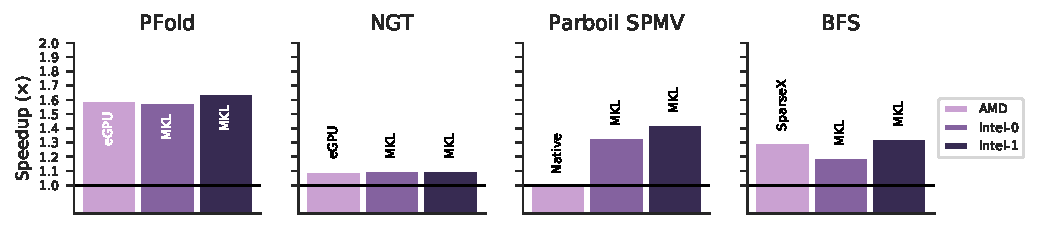
\includegraphics[width=\linewidth]{figures/baseline.pdf}
  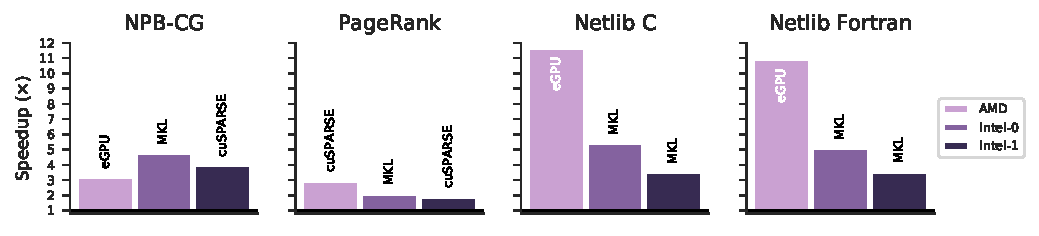
\includegraphics[width=\linewidth]{figures/baseline_bench.pdf}
\\[-0.75em]
  \caption{Evaluation on real-world application code and well-known benchmark
          suites:
           Bars show geometric mean speedup of best-performing LiLAC harness across the
           set of input examples for each benchmark and platform. }
  \label{spmv_app_perf}
\end{figure*}

The speedups that LiLAC achieves on real applications as well as benchmarks are
shown in \autoref{spmv_app_perf}.
They range from $1.1$--$3\times$ on the scientific application codes to
12$\times$ on well-known sparse benchmark programs.

On the \textsc{pathsample} applications (PFold and NGT), we measured
consistent speedups of approximately 50$\%$ and 10$\%$ respectively across
all 3 platforms.
For large applications, Amdahl's law is a severe limitation for
approaches like ours --- other parts of the applications dominate execution
times when linear algebra is accelerated.

PageRank requires a large number of SPMV calls using the same input matrix to
iterate until convergence.
The GPU implementations running on AMD and Intel-1 are able to take advantage of
data remaining in memory.
The larger number of CPU cores and slower GPU available on \mbox{Intel-0} make
MKL its best-performing implementation.
CPU implementations perform best on BFS by avoiding memory copies entirely
--- on AMD, SparseX outperforms GPU implementations.

On standard sparse linear algebra benchmarks, LiLAC achieves speedups of up to
$12\times$.
The impact is independent of the source language, as the C and FORTRAN versions
of the Netlib benchmark demonstrate.
LiLAC is able to achieve consistent, useful speedups across a variety of
hardware configurations.

    \autoref{fig:performance-distribution} demonstrates that achieving good
    performance independent of the hardware platform is no small feat.
    It shows the distribution of speedups on the NPB-CG benchmark across
    different machines, problem sizes and linear algebra implementation.
    More detailed performance data is in \autoref{tab:perf_data}.
    The best-performing implementation varies considerably, depending on
    characteristics of the problem in question.
    No accelerator library performs well reliably, each harness outperforms
    any other harness on some combination of data set and platform.
    clSPARSE on the AMD iGPU is the only harness that is consistently
    outperformed.

\begin{table*}[t]
  \centering
  \footnotesize
  \begin{tabular}{ll|ccc|ccc|ccc|ccc}
    \multirow{2}{*}{\textbf{Platform}} &
    \multirow{2}{*}{\textbf{Implementation}} &
    \multicolumn{3}{c}{\textbf{PFold}} & \multicolumn{3}{c}{\textbf{NGT}} &
    \multicolumn{3}{c}{\textbf{PageRank}} & \multicolumn{3}{c}{\textbf{BFS}} \\[-0.3em]
    & & \hspace{0.8em}L0\hspace{0.8em} & \hspace{0.8em}L1\hspace{0.8em} & \hspace{0.8em}L2\hspace{0.8em}
      & \hspace{0.8em}L0\hspace{0.8em} & \hspace{0.8em}L1\hspace{0.8em} & \hspace{0.8em}L2\hspace{0.8em}
      & \hspace{0.35em}Erdos\hspace{0.35em} & LJ-2008 & \hspace{0.35em}Road\hspace{0.35em}
      & \hspace{0.35em}Erdos\hspace{0.35em} & LJ-2008 & \hspace{0.35em}Road\hspace{0.35em} \\
    \hline
    \hline
    \multirow{3}{*}{Intel-0} 
    & MKL & 2.88 & 2.46 & 1.00 & 1.18 & 1.18 & 1.18 & 1.25 & 2.93 & 1.72 & 2.50 & 1.06 & 1.05 \\[-0.3em]
    & cuSPARSE & 0.75 & 0.60 & 0.45 & 0.66 & 0.66 & 0.66 & 1.39 & 1.00 & 3.32 & 0.87 & 1.74 & 1.28 \\[-0.3em]
    & clSPARSE & 0.90 & 0.75 & 0.46 & 0.81 & 0.79 & 0.78 & 1.24 & 0.95 & 2.24 & 0.13 & 1.45 & 0.07 \\[-0.3em]
    & SparseX & - & - & - & - & - & - & - & - & - & 1.19 & - & - \\
    \hline
    \multirow{3}{*}{Intel-1}
    & MKL & 2.70 & 2.43 & 1.01 & 1.20 & 1.20 & 1.19 & 1.63 & 1.03 & 2.26 & 1.06 & 2.09 & 1.27 \\[-0.3em]
    & cuSPARSE & 0.48 & 0.41 & 0.30 & 0.68 & 0.69 & 0.68 & 1.59 & 0.87 & 4.44 & 1.01 & 1.83 & 1.63 \\[-0.3em]
    & clSPARSE & 1.00 & 1.00 & 1.00 & 1.00 & 1.02 & 1.00 & 1.50 & 0.87 & 3.46 & 0.23 & 1.81 & 0.13 \\[-0.3em]
    & SparseX & - & - & - & - & - & - & - & - & - & 1.25 & - & - \\
    \hline
    \multirow{4}{*}{AMD}
    & cuSPARSE & 1.38 & 1.18 & 0.67 & 0.69 & 0.69 & 0.70 & 3.44 & 1.18 & 9.97 & 1.62 & 6.55 & 1.96 \\[-0.3em]
    & clSPARSE (eGPU) & 2.17 & 1.82 & 1.22 & 1.16 & 1.16 & 1.16 & 3.08 & 1.24 & 6.06 & 0.50 & 11.03 & 0.24 \\[-0.3em]
    & clSPARSE (iGPU) & 2.03 & 1.78 & 1.03 & 0.90 & 0.90 & 0.90 & 3.26 & 1.31 & 4.05 & 0.14 & 4.17 & 0.05 \\[-0.3em]
    & SparseX & - & - & - & - & - & - & - & - & - & 1.93 & - & - \\
  \end{tabular}
\vspace{0.5em}
  \caption{LiLAC speedups on each platform, across different applications and
  problem sizes.
  SparseX demonstrated promising performance on some applications, but we were
  unable to evaluate on every relevant instance due to instability.}
  \label{tab:perf_data}
\vspace{-2em}
\end{table*}

\begin{figure}[t]
  \centering
  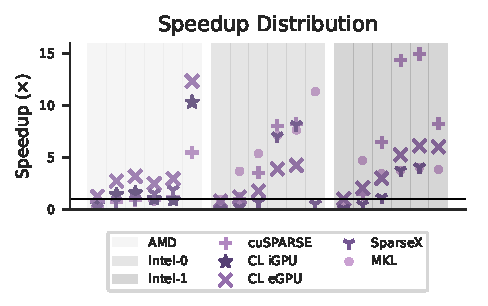
\includegraphics[width=\columnwidth,height=0.67\columnwidth]{figures/distribution.pdf}
\\[-0.75em]
  \caption{Distribution of speedups achieved by LiLAC on the NPB-CG benchmark.
    Each column of points shows the speedup achieved by each implementation
    available on a platform for a particular problem size. Data is sorted along
  the $x$-axis by the best speedup in that column.}
  \label{fig:performance-distribution}
\end{figure}

We verify that LiLAC can reach near-optimal performance, despite using general
and portable harnesses, by comparing the achieved speedups with the performance
of reference implementations.
This was possible on the NPB and Parboil benchmarks, where expert hand
crafted version are available that achieve close to peak performance.


\autoref{tab:lilac-linesofcode} shows our results from these experiments.
For context, we also measure application programmer effort for peak performance,
which is substantial, requiring hundreds of lines of carefully crafted
high performance OpenCL code.
On the NPB-CG benchmark, we achieve $\sim 3\times$ speedup,
while the expert implementation is approximately 3$\times$ faster than LiLAC.
This is partly due to Amdahl's law --- the benchmark also performs operations
other than sparse matrix-vector multiplication and the expert implementation is
a complete rewrite that performs all these operations on the GPU.
On Parboil SPMV, the difference between an expert and LiLAC is only
1.07$\times$.

\begin{figure}[t]
  \centering
  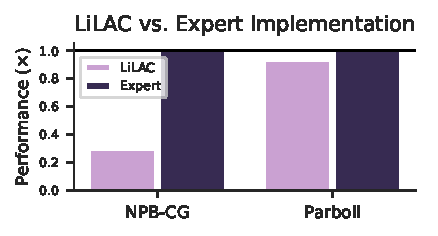
\includegraphics[width=0.9\columnwidth,height=0.5\columnwidth]{figures/expert.pdf}
\\[0.5em]
  \begin{tabular}{lrr}
    \multirow{2}{*}{\textbf{Benchmark}} & \multicolumn{2}{c}{\textbf{Modified LoC}} \\
    & LiLAC & Expert \\
    \toprule
    \toprule
    NPB          & 0 (44) & 1948 \\
    Parboil SPMV & 0 (44) & 261
  \end{tabular}
\\[0.45em]
  \caption{LiLAC vs Expert: We achieve good performance with no application
           programmer effort (measured as required LoC change).
           LiLAC code to be written by library developers is in parentheses.
           Amdahl's Law limits our impact on NPB.
}
  \label{tab:lilac-linesofcode}
\end{figure}

After moving the burden of targeting accelerators from the user to the
library vendor with LiLAC, we would also like to automate the selection of which
library to use.
This may change over time and per application, as we saw in
\autoref{fig:performance-distribution}.
We have experimented with simple classifiers for each platform, that dynamically
select the best library given the data input.
This was straightforward to achieve for our problem space, but more data is
needed for a meaningful evaluation, and we leave it to future work.


\subsection{Effectiveness of Data Marshaling}
Our implementation of LiLAC relies on a non-trivial data marshaling system that
prevents redundant computations and memory transfers. We present performance
results that show the importance and effectiveness of this system.

\begin{figure}[t]
  \centering
  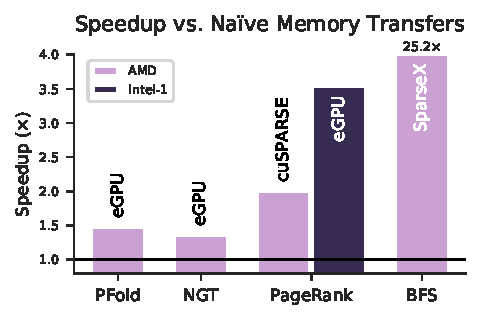
\includegraphics[width=\columnwidth,height=0.67\columnwidth]{figures/marshall.pdf}
\\[-0.75em]
  \caption{LiLAC vs. na\"ive library calls without harnesses.
           Avoiding memory transfers is necessary for performance.}
  \label{fig:transfer-performance}
\end{figure}

We repeated our experiments, using the best-performing implementations from
\autoref{spmv_app_perf}.
Instead of using our data marshaling scheme, we transfer memory naively for
each accelerator invocation.
We then measured the performance advantage that our harness system gives us over
this naive approach, results are in \autoref{fig:transfer-performance}.
The GPU implementations received speedups of 1.4--3.5$\times$ and SparseX was
sped up by over $25\times$ (because it performs an internal matrix tuning phase
that is far more expensive than a memory copy).
These speedups are large enough that in each case, the application would in fact
have performed worse than their sequential baselines without performing data
marshaling.

\begin{table}[b]
\centering
\caption{Sparsity does not fit the polyhedral model, Intel compilers fail to
         parallelize and Polly is not available for FORTRAN.
         Only LiLAC detects sparse linear algebra reliably.}
\label{compareiccpolly}
\vspace{-0.5em}
\small
\begin{tabular}{l|c|c|c}
{\bf Benchmark}      & {\bf LiLAC}    & {\bf Polly}   & {\bf Intel icc/ifort} \\
\hline
\hline
PFold          & CSR & - & parallel dependence \\[-0.3em]
NGT            & CSR & - & parallel dependence \\[-0.3em]
Parboil-SPMV   & JDS & no SCoP & parallel dependence \\[-0.3em]
BFS            & CSR & no SCoP & parallel dependence \\[-0.3em]
NPB-CG         & CSR & - & parallel dependence \\[-0.3em]
PageRank       & CSR & no SCoP & parallel dependence \\[-0.3em]
Netlib C       & CSR & no SCoP & parallel dependence \\[-0.3em]
Netlib Fortran & CSR & - & parallel dependence \\
\end{tabular}
\end{table}

\subsection{Reliability of Discovery}

    To achieve performance impact, LiLAC needs to reliably detect linear algebra
    computations, independent of coding style and source programming language.
    The results so far demonstrated that this works reliably and the data in
    \autoref{compareiccpolly} reiterates this.
    Established approaches, like the polyhedral model, on the otehr hand, are
    unable to model sparse linear algebra.
    We verified this with the Polly compiler and found that no SCoPs captured
    sparse linear algebra.
    This is unsurprising, as the basic assumptions of affine memory access are
    contradicted by the indirection that is inherent in sparsity.
    Similarly, the Intel icc and ifort compilers fail to auto-parallelize, as
    they cannot reason about sparsity and have to assume additional dependencies
    where sparse accesses occur.


\section{Conclusion}
\label{sec:conclusion}
% Sparse and dense linear algebra are critical workloads for many important
% established applications and will only gain more significance with emerging
% domains such as deep learning and AI.

% Past experience has shown that acceleration solutions that require even limited
% modifications of legacy source code hinder mainstream adoption.
% Hence, the providion of custom APIs for new accelerator hardware is insufficient
% to penetrate scientific computing outside of elite projects.
% At the same time, entirely compiler based solution have failed to scale and
% perform.

% We have demonstrated that our approach of compiler based detection coupled with
% library based acceleration manages to combine the advantages of both, achieving
% the full performance without requiring programmer intervention.
% We showed that this scales to large scientific codes across multiple programming
% languages.

This paper has presented LiLAC, a language and compiler that enables existing
code bases to exploit sparse (and dense) linear algebra accelerator libraries.
No effort is required from the application programmer.
Instead, the library implementer provides a few lines of specification, which
LiLAC uses to  automatically and efficiently matches  user code to
underlying high performance libraries.

We demonstrated this approach on  C, C++ and FORTRAN benchmarks as well as
legacy applications and shown significant performance improvement across
platforms and data sets.
Many language features of the LiLAC language could be repurposed for libraries
beyond linear algebra.
In future work, we will investigate how our framework could be adapted to other
application domains, enabling effort free access to an even larger set of
accelerator libraries.



\chapter{Conclusion}

\bibliographystyle{plainnat}
\bibliography{references}
\end{document}
